\batchmode
\documentclass{article}
\RequirePackage{ifthen}


\usepackage[english]{babel}
\usepackage{geometry,amsmath,amssymb,graphicx,bbm}
\geometry{a4paper}

%
\providecommand{\nobracket}{}%
\providecommand{\tmaffiliation}[1]{\\#1}%
\providecommand{\tmmathbf}[1]{\ensuremath{\boldsymbol{#1}}}%
\providecommand{\tmop}[1]{\ensuremath{\operatorname{#1}}}%
\providecommand{\tmtextit}[1]{{\itshape{#1}}} 




\usepackage[dvips]{color}


\pagecolor[gray]{.7}

\usepackage[latin1]{inputenc}



\makeatletter

\makeatletter
\count@=\the\catcode`\_ \catcode`\_=8 
\newenvironment{tex2html_wrap}{}{}%
\catcode`\<=12\catcode`\_=\count@
\newcommand{\providedcommand}[1]{\expandafter\providecommand\csname #1\endcsname}%
\newcommand{\renewedcommand}[1]{\expandafter\providecommand\csname #1\endcsname{}%
  \expandafter\renewcommand\csname #1\endcsname}%
\newcommand{\newedenvironment}[1]{\newenvironment{#1}{}{}\renewenvironment{#1}}%
\let\newedcommand\renewedcommand
\let\renewedenvironment\newedenvironment
\makeatother
\let\mathon=$
\let\mathoff=$
\ifx\AtBeginDocument\undefined \newcommand{\AtBeginDocument}[1]{}\fi
\newbox\sizebox
\setlength{\hoffset}{0pt}\setlength{\voffset}{0pt}
\addtolength{\textheight}{\footskip}\setlength{\footskip}{0pt}
\addtolength{\textheight}{\topmargin}\setlength{\topmargin}{0pt}
\addtolength{\textheight}{\headheight}\setlength{\headheight}{0pt}
\addtolength{\textheight}{\headsep}\setlength{\headsep}{0pt}
\setlength{\textwidth}{349pt}
\newwrite\lthtmlwrite
\makeatletter
\let\realnormalsize=\normalsize
\global\topskip=2sp
\def\preveqno{}\let\real@float=\@float \let\realend@float=\end@float
\def\@float{\let\@savefreelist\@freelist\real@float}
\def\liih@math{\ifmmode$\else\bad@math\fi}
\def\end@float{\realend@float\global\let\@freelist\@savefreelist}
\let\real@dbflt=\@dbflt \let\end@dblfloat=\end@float
\let\@largefloatcheck=\relax
\let\if@boxedmulticols=\iftrue
\def\@dbflt{\let\@savefreelist\@freelist\real@dbflt}
\def\adjustnormalsize{\def\normalsize{\mathsurround=0pt \realnormalsize
 \parindent=0pt\abovedisplayskip=0pt\belowdisplayskip=0pt}%
 \def\phantompar{\csname par\endcsname}\normalsize}%
\def\lthtmltypeout#1{{\let\protect\string \immediate\write\lthtmlwrite{#1}}}%
\newcommand\lthtmlhboxmathA{\adjustnormalsize\setbox\sizebox=\hbox\bgroup\kern.05em }%
\newcommand\lthtmlhboxmathB{\adjustnormalsize\setbox\sizebox=\hbox to\hsize\bgroup\hfill }%
\newcommand\lthtmlvboxmathA{\adjustnormalsize\setbox\sizebox=\vbox\bgroup %
 \let\ifinner=\iffalse \let\)\liih@math }%
\newcommand\lthtmlboxmathZ{\@next\next\@currlist{}{\def\next{\voidb@x}}%
 \expandafter\box\next\egroup}%
\newcommand\lthtmlmathtype[1]{\gdef\lthtmlmathenv{#1}}%
\newcommand\lthtmllogmath{\dimen0\ht\sizebox \advance\dimen0\dp\sizebox
  \ifdim\dimen0>.95\vsize
   \lthtmltypeout{%
*** image for \lthtmlmathenv\space is too tall at \the\dimen0, reducing to .95 vsize ***}%
   \ht\sizebox.95\vsize \dp\sizebox\z@ \fi
  \lthtmltypeout{l2hSize %
:\lthtmlmathenv:\the\ht\sizebox::\the\dp\sizebox::\the\wd\sizebox.\preveqno}}%
\newcommand\lthtmlfigureA[1]{\let\@savefreelist\@freelist
       \lthtmlmathtype{#1}\lthtmlvboxmathA}%
\newcommand\lthtmlpictureA{\bgroup\catcode`\_=8 \lthtmlpictureB}%
\newcommand\lthtmlpictureB[1]{\lthtmlmathtype{#1}\egroup
       \let\@savefreelist\@freelist \lthtmlhboxmathB}%
\newcommand\lthtmlpictureZ[1]{\hfill\lthtmlfigureZ}%
\newcommand\lthtmlfigureZ{\lthtmlboxmathZ\lthtmllogmath\copy\sizebox
       \global\let\@freelist\@savefreelist}%
\newcommand\lthtmldisplayA{\bgroup\catcode`\_=8 \lthtmldisplayAi}%
\newcommand\lthtmldisplayAi[1]{\lthtmlmathtype{#1}\egroup\lthtmlvboxmathA}%
\newcommand\lthtmldisplayB[1]{\edef\preveqno{(\theequation)}%
  \lthtmldisplayA{#1}\let\@eqnnum\relax}%
\newcommand\lthtmldisplayZ{\lthtmlboxmathZ\lthtmllogmath\lthtmlsetmath}%
\newcommand\lthtmlinlinemathA{\bgroup\catcode`\_=8 \lthtmlinlinemathB}
\newcommand\lthtmlinlinemathB[1]{\lthtmlmathtype{#1}\egroup\lthtmlhboxmathA
  \vrule height1.5ex width0pt }%
\newcommand\lthtmlinlineA{\bgroup\catcode`\_=8 \lthtmlinlineB}%
\newcommand\lthtmlinlineB[1]{\lthtmlmathtype{#1}\egroup\lthtmlhboxmathA}%
\newcommand\lthtmlinlineZ{\egroup\expandafter\ifdim\dp\sizebox>0pt %
  \expandafter\centerinlinemath\fi\lthtmllogmath\lthtmlsetinline}
\newcommand\lthtmlinlinemathZ{\egroup\expandafter\ifdim\dp\sizebox>0pt %
  \expandafter\centerinlinemath\fi\lthtmllogmath\lthtmlsetmath}
\newcommand\lthtmlindisplaymathZ{\egroup %
  \centerinlinemath\lthtmllogmath\lthtmlsetmath}
\def\lthtmlsetinline{\hbox{\vrule width.1em \vtop{\vbox{%
  \kern.1em\copy\sizebox}\ifdim\dp\sizebox>0pt\kern.1em\else\kern.3pt\fi
  \ifdim\hsize>\wd\sizebox \hrule depth1pt\fi}}}
\def\lthtmlsetmath{\hbox{\vrule width.1em\kern-.05em\vtop{\vbox{%
  \kern.1em\kern0.8 pt\hbox{\hglue.17em\copy\sizebox\hglue0.8 pt}}\kern.3pt%
  \ifdim\dp\sizebox>0pt\kern.1em\fi \kern0.8 pt%
  \ifdim\hsize>\wd\sizebox \hrule depth1pt\fi}}}
\def\centerinlinemath{%
  \dimen1=\ifdim\ht\sizebox<\dp\sizebox \dp\sizebox\else\ht\sizebox\fi
  \advance\dimen1by.5pt \vrule width0pt height\dimen1 depth\dimen1 
 \dp\sizebox=\dimen1\ht\sizebox=\dimen1\relax}

\def\lthtmlcheckvsize{\ifdim\ht\sizebox<\vsize 
  \ifdim\wd\sizebox<\hsize\expandafter\hfill\fi \expandafter\vfill
  \else\expandafter\vss\fi}%
\providecommand{\selectlanguage}[1]{}%
\makeatletter \tracingstats = 1 
\providecommand{\Nu}{\textrm{N}}
\providecommand{\Iota}{\textrm{J}}
\providecommand{\Epsilon}{\textrm{E}}
\providecommand{\Zeta}{\textrm{Z}}
\providecommand{\Kappa}{\textrm{K}}
\providecommand{\Eta}{\textrm{H}}
\providecommand{\omicron}{\textrm{o}}
\providecommand{\Alpha}{\textrm{A}}
\providecommand{\Mu}{\textrm{M}}
\providecommand{\Omicron}{\textrm{O}}
\providecommand{\Beta}{\textrm{B}}
\providecommand{\Rho}{\textrm{R}}
\providecommand{\Tau}{\textrm{T}}
\providecommand{\Chi}{\textrm{X}}


\begin{document}
\pagestyle{empty}\thispagestyle{empty}\lthtmltypeout{}%
\lthtmltypeout{latex2htmlLength hsize=\the\hsize}\lthtmltypeout{}%
\lthtmltypeout{latex2htmlLength vsize=\the\vsize}\lthtmltypeout{}%
\lthtmltypeout{latex2htmlLength hoffset=\the\hoffset}\lthtmltypeout{}%
\lthtmltypeout{latex2htmlLength voffset=\the\voffset}\lthtmltypeout{}%
\lthtmltypeout{latex2htmlLength topmargin=\the\topmargin}\lthtmltypeout{}%
\lthtmltypeout{latex2htmlLength topskip=\the\topskip}\lthtmltypeout{}%
\lthtmltypeout{latex2htmlLength headheight=\the\headheight}\lthtmltypeout{}%
\lthtmltypeout{latex2htmlLength headsep=\the\headsep}\lthtmltypeout{}%
\lthtmltypeout{latex2htmlLength parskip=\the\parskip}\lthtmltypeout{}%
\lthtmltypeout{latex2htmlLength oddsidemargin=\the\oddsidemargin}\lthtmltypeout{}%
\makeatletter
\if@twoside\lthtmltypeout{latex2htmlLength evensidemargin=\the\evensidemargin}%
\else\lthtmltypeout{latex2htmlLength evensidemargin=\the\oddsidemargin}\fi%
\lthtmltypeout{}%
\makeatother
\setcounter{page}{1}
\onecolumn

% !!! IMAGES START HERE !!!

{\newpage\clearpage
\lthtmlinlinemathA{tex2html_wrap_inline15798}%
$ \Psi $%
\lthtmlinlinemathZ
\lthtmlcheckvsize\clearpage}

{\newpage\clearpage
\lthtmlinlinemathA{tex2html_wrap_inline15804}%
$ (R, Z)$%
\lthtmlinlinemathZ
\lthtmlcheckvsize\clearpage}

{\newpage\clearpage
\lthtmlinlinemathA{tex2html_wrap_inline15806}%
$ Z$%
\lthtmlinlinemathZ
\lthtmlcheckvsize\clearpage}

{\newpage\clearpage
\lthtmlinlinemathA{tex2html_wrap_inline15828}%
$ \Psi _p$%
\lthtmlinlinemathZ
\lthtmlcheckvsize\clearpage}

{\newpage\clearpage
\lthtmlinlinemathA{tex2html_wrap_inline15830}%
$ \Psi _1$%
\lthtmlinlinemathZ
\lthtmlcheckvsize\clearpage}

{\newpage\clearpage
\lthtmlinlinemathA{tex2html_wrap_inline15832}%
$ \Psi _2$%
\lthtmlinlinemathZ
\lthtmlcheckvsize\clearpage}

{\newpage\clearpage
\lthtmlinlinemathA{tex2html_wrap_inline15834}%
$ \Psi _p = 2 \pi (\Psi _2 - \Psi _1)$%
\lthtmlinlinemathZ
\lthtmlcheckvsize\clearpage}

{\newpage\clearpage
\lthtmlinlinemathA{tex2html_wrap_inline15848}%
$ S_2$%
\lthtmlinlinemathZ
\lthtmlcheckvsize\clearpage}

{\newpage\clearpage
\lthtmlinlinemathA{tex2html_wrap_inline15850}%
$ S_3$%
\lthtmlinlinemathZ
\lthtmlcheckvsize\clearpage}

{\newpage\clearpage
\lthtmlinlinemathA{tex2html_wrap_inline15852}%
$ S_4$%
\lthtmlinlinemathZ
\lthtmlcheckvsize\clearpage}

{\newpage\clearpage
\lthtmlinlinemathA{tex2html_wrap_inline15854}%
$ S_5$%
\lthtmlinlinemathZ
\lthtmlcheckvsize\clearpage}

{\newpage\clearpage
\lthtmlinlinemathA{tex2html_wrap_inline15856}%
$ S_0$%
\lthtmlinlinemathZ
\lthtmlcheckvsize\clearpage}

{\newpage\clearpage
\lthtmlinlinemathA{tex2html_wrap_inline15858}%
$ S_1$%
\lthtmlinlinemathZ
\lthtmlcheckvsize\clearpage}

{\newpage\clearpage
\lthtmlinlinemathA{tex2html_wrap_inline15878}%
$ R$%
\lthtmlinlinemathZ
\lthtmlcheckvsize\clearpage}

{\newpage\clearpage
\lthtmlinlinemathA{tex2html_wrap_inline15880}%
$ R_{\ensuremath  {\operatorname  {in}}}$%
\lthtmlinlinemathZ
\lthtmlcheckvsize\clearpage}

{\newpage\clearpage
\lthtmlinlinemathA{tex2html_wrap_inline15882}%
$ R_{\ensuremath  {\operatorname  {out}}}$%
\lthtmlinlinemathZ
\lthtmlcheckvsize\clearpage}

{\newpage\clearpage
\lthtmlinlinemathA{tex2html_wrap_inline15886}%
$ (R_{\ensuremath  {\operatorname  {top}}}, Z_{\ensuremath  {\operatorname  {top}}})$%
\lthtmlinlinemathZ
\lthtmlcheckvsize\clearpage}

{\newpage\clearpage
\lthtmlinlinemathA{tex2html_wrap_inline15892}%
$ q = 2.1 = 21 / 10$%
\lthtmlinlinemathZ
\lthtmlcheckvsize\clearpage}

{\newpage\clearpage
\lthtmlinlinemathA{tex2html_wrap_inline15894}%
$ \phi = 0$%
\lthtmlinlinemathZ
\lthtmlcheckvsize\clearpage}

{\newpage\clearpage
\lthtmlinlinemathA{tex2html_wrap_inline15898}%
$ g$%
\lthtmlinlinemathZ
\lthtmlcheckvsize\clearpage}

{\newpage\clearpage
\lthtmlinlinemathA{tex2html_wrap_inline15920}%
$ \kappa _0 = 1.5$%
\lthtmlinlinemathZ
\lthtmlcheckvsize\clearpage}

{\newpage\clearpage
\lthtmlinlinemathA{tex2html_wrap_inline15922}%
$ q_0 = 1.5$%
\lthtmlinlinemathZ
\lthtmlcheckvsize\clearpage}

{\newpage\clearpage
\lthtmlinlinemathA{tex2html_wrap_inline15924}%
$ \overline  {\Psi }$%
\lthtmlinlinemathZ
\lthtmlcheckvsize\clearpage}

{\newpage\clearpage
\lthtmlinlinemathA{tex2html_wrap_inline15928}%
$ \overline  {R}$%
\lthtmlinlinemathZ
\lthtmlcheckvsize\clearpage}

{\newpage\clearpage
\lthtmlinlinemathA{tex2html_wrap_inline15930}%
$ R = 0$%
\lthtmlinlinemathZ
\lthtmlcheckvsize\clearpage}

{\newpage\clearpage
\lthtmlinlinemathA{tex2html_wrap_inline15934}%
$ 0.123 - \varepsilon $%
\lthtmlinlinemathZ
\lthtmlcheckvsize\clearpage}

{\newpage\clearpage
\lthtmlinlinemathA{tex2html_wrap_inline15936}%
$ \varepsilon $%
\lthtmlinlinemathZ
\lthtmlcheckvsize\clearpage}

{\newpage\clearpage
\lthtmlinlinemathA{tex2html_wrap_inline15938}%
$ \varepsilon = 10^{- 3}$%
\lthtmlinlinemathZ
\lthtmlcheckvsize\clearpage}

{\newpage\clearpage
\lthtmlinlinemathA{tex2html_wrap_inline15942}%
$ \psi , \theta , \zeta $%
\lthtmlinlinemathZ
\lthtmlcheckvsize\clearpage}

{\newpage\clearpage
\lthtmlinlinemathA{tex2html_wrap_inline15946}%
$ (\psi , \theta , \zeta )$%
\lthtmlinlinemathZ
\lthtmlcheckvsize\clearpage}

{\newpage\clearpage
\lthtmlinlinemathA{tex2html_wrap_inline15962}%
$ (\psi , \theta , \phi )$%
\lthtmlinlinemathZ
\lthtmlcheckvsize\clearpage}

{\newpage\clearpage
\lthtmlinlinemathA{tex2html_wrap_inline15970}%
$ \theta $%
\lthtmlinlinemathZ
\lthtmlcheckvsize\clearpage}

{\newpage\clearpage
\lthtmlinlinemathA{tex2html_wrap_inline15990}%
$ \sqrt  {\overline  {\Psi }_t} = 0.01714$%
\lthtmlinlinemathZ
\lthtmlcheckvsize\clearpage}

{\newpage\clearpage
\lthtmlinlinemathA{tex2html_wrap_inline15992}%
$ \sqrt  {\overline  {\Psi }_t} = 0.9851$%
\lthtmlinlinemathZ
\lthtmlcheckvsize\clearpage}

{\newpage\clearpage
\lthtmlinlinemathA{tex2html_wrap_inline15994}%
$ \sqrt  {\overline  {\Psi }_t}$%
\lthtmlinlinemathZ
\lthtmlcheckvsize\clearpage}

{\newpage\clearpage
\lthtmlinlinemathA{tex2html_wrap_inline15998}%
$ \Psi (R, Z)$%
\lthtmlinlinemathZ
\lthtmlcheckvsize\clearpage}

{\newpage\clearpage
\lthtmlinlinemathA{tex2html_wrap_inline16008}%
$ | \nabla \Psi |$%
\lthtmlinlinemathZ
\lthtmlcheckvsize\clearpage}

{\newpage\clearpage
\lthtmlinlinemathA{tex2html_wrap_inline16016}%
$ B_p = | \nabla \Psi | / R$%
\lthtmlinlinemathZ
\lthtmlcheckvsize\clearpage}

{\newpage\clearpage
\lthtmlinlinemathA{tex2html_wrap_inline16018}%
$ B_{\phi } = g / R$%
\lthtmlinlinemathZ
\lthtmlcheckvsize\clearpage}

{\newpage\clearpage
\lthtmlinlinemathA{tex2html_wrap_inline16038}%
$ (\psi , \theta , \zeta ) \ensuremath  {\operatorname  {with}}$%
\lthtmlinlinemathZ
\lthtmlcheckvsize\clearpage}

{\newpage\clearpage
\lthtmlinlinemathA{tex2html_wrap_inline16040}%
$ \zeta $%
\lthtmlinlinemathZ
\lthtmlcheckvsize\clearpage}

{\newpage\clearpage
\lthtmlinlinemathA{tex2html_wrap_inline16062}%
$ B \cdot \nabla $%
\lthtmlinlinemathZ
\lthtmlcheckvsize\clearpage}

{\newpage\clearpage
\lthtmlinlinemathA{tex2html_wrap_inline16074}%
$ (B \times \nabla \psi / B^2) \cdot \nabla $%
\lthtmlinlinemathZ
\lthtmlcheckvsize\clearpage}

{\newpage\clearpage
\lthtmlinlinemathA{tex2html_wrap_inline16080}%
$ (\psi , \theta , \alpha )$%
\lthtmlinlinemathZ
\lthtmlcheckvsize\clearpage}

{\newpage\clearpage
\lthtmlinlinemathA{tex2html_wrap_inline16090}%
$ \alpha $%
\lthtmlinlinemathZ
\lthtmlcheckvsize\clearpage}

{\newpage\clearpage
\lthtmlinlinemathA{tex2html_wrap_inline16116}%
$ \theta = 9 \times 2 \pi / 63$%
\lthtmlinlinemathZ
\lthtmlcheckvsize\clearpage}

{\newpage\clearpage
\lthtmlinlinemathA{tex2html_wrap_inline16120}%
$ \psi $%
\lthtmlinlinemathZ
\lthtmlcheckvsize\clearpage}

{\newpage\clearpage
\lthtmlinlinemathA{tex2html_wrap_inline16122}%
$ \partial \mathbf  {r}/ \partial \psi $%
\lthtmlinlinemathZ
\lthtmlcheckvsize\clearpage}

{\newpage\clearpage
\lthtmlinlinemathA{tex2html_wrap_inline16130}%
$ \partial \mathbf  {r}/ \partial \alpha $%
\lthtmlinlinemathZ
\lthtmlcheckvsize\clearpage}

{\newpage\clearpage
\lthtmlinlinemathA{tex2html_wrap_inline16132}%
$ \mathaccentV {hat}05E{\ensuremath  {\boldsymbol  {\phi }}}$%
\lthtmlinlinemathZ
\lthtmlcheckvsize\clearpage}

{\newpage\clearpage
\lthtmlinlinemathA{tex2html_wrap_inline16156}%
$ \theta = 19 \times 2 \pi / 63$%
\lthtmlinlinemathZ
\lthtmlcheckvsize\clearpage}

{\newpage\clearpage
\lthtmlinlinemathA{tex2html_wrap_inline16168}%
$ \partial \mathbf  {r}/ \partial \phi $%
\lthtmlinlinemathZ
\lthtmlcheckvsize\clearpage}

{\newpage\clearpage
\lthtmlinlinemathA{tex2html_wrap_inline16200}%
$ \theta = 0$%
\lthtmlinlinemathZ
\lthtmlcheckvsize\clearpage}

{\newpage\clearpage
\lthtmlinlinemathA{tex2html_wrap_inline16204}%
$ \partial \mathbf  {r}/ \partial \psi |_{\theta , \alpha } $%
\lthtmlinlinemathZ
\lthtmlcheckvsize\clearpage}

{\newpage\clearpage
\lthtmlinlinemathA{tex2html_wrap_inline16206}%
$ \alpha _j = j 2 \pi / 20$%
\lthtmlinlinemathZ
\lthtmlcheckvsize\clearpage}

{\newpage\clearpage
\lthtmlinlinemathA{tex2html_wrap_inline16208}%
$ j = 0, 1, 2, \ldots  , 20$%
\lthtmlinlinemathZ
\lthtmlcheckvsize\clearpage}

{\newpage\clearpage
\lthtmlinlinemathA{tex2html_wrap_inline16214}%
$ \alpha = 0$%
\lthtmlinlinemathZ
\lthtmlcheckvsize\clearpage}

{\newpage\clearpage
\lthtmlinlinemathA{tex2html_wrap_inline16216}%
$ \theta = 2 \pi $%
\lthtmlinlinemathZ
\lthtmlcheckvsize\clearpage}

{\newpage\clearpage
\lthtmlinlinemathA{tex2html_wrap_inline16218}%
$ (q_{\qopname  \relax m{max}} - q_{\qopname  \relax m{min}}) 2 \pi = (5.56 - 1.79) \times 2 \pi \approx 4 \times 2 \pi $%
\lthtmlinlinemathZ
\lthtmlcheckvsize\clearpage}

{\newpage\clearpage
\lthtmlinlinemathA{tex2html_wrap_inline16220}%
$ \psi = 0.2 \rightarrow 0.9$%
\lthtmlinlinemathZ
\lthtmlcheckvsize\clearpage}

{\newpage\clearpage
\lthtmlinlinemathA{tex2html_wrap_inline16236}%
$ \psi = 0.2$%
\lthtmlinlinemathZ
\lthtmlcheckvsize\clearpage}

{\newpage\clearpage
\lthtmlinlinemathA{tex2html_wrap_inline16240}%
$ \Delta \theta = 2 \pi $%
\lthtmlinlinemathZ
\lthtmlcheckvsize\clearpage}

{\newpage\clearpage
\lthtmlinlinemathA{tex2html_wrap_inline16242}%
$ q = 1.79$%
\lthtmlinlinemathZ
\lthtmlcheckvsize\clearpage}

{\newpage\clearpage
\lthtmlinlinemathA{tex2html_wrap_inline16270}%
$ \phi $%
\lthtmlinlinemathZ
\lthtmlcheckvsize\clearpage}

{\newpage\clearpage
\lthtmlinlinemathA{tex2html_wrap_inline16276}%
$ \phi _j = \alpha _j = (j - 1) 2 \pi / 4 / (10 - 1)$%
\lthtmlinlinemathZ
\lthtmlcheckvsize\clearpage}

{\newpage\clearpage
\lthtmlinlinemathA{tex2html_wrap_inline16278}%
$ j = 1, 2, \ldots  , 10$%
\lthtmlinlinemathZ
\lthtmlcheckvsize\clearpage}

{\newpage\clearpage
\lthtmlinlinemathA{tex2html_wrap_inline16280}%
$ 1 / 4$%
\lthtmlinlinemathZ
\lthtmlcheckvsize\clearpage}

{\newpage\clearpage
\lthtmlinlinemathA{tex2html_wrap_inline16284}%
$ \alpha _j = (j - 1) 2 \pi / 4 / (10 - 1)$%
\lthtmlinlinemathZ
\lthtmlcheckvsize\clearpage}

{\newpage\clearpage
\lthtmlinlinemathA{tex2html_wrap_inline16290}%
$ 2 \pi $%
\lthtmlinlinemathZ
\lthtmlcheckvsize\clearpage}

{\newpage\clearpage
\lthtmlinlinemathA{tex2html_wrap_inline16320}%
$ d \alpha = 2 \pi / 20$%
\lthtmlinlinemathZ
\lthtmlcheckvsize\clearpage}

{\newpage\clearpage
\lthtmlinlinemathA{tex2html_wrap_inline16344}%
$ \phi = 2 \pi / 8$%
\lthtmlinlinemathZ
\lthtmlcheckvsize\clearpage}

{\newpage\clearpage
\lthtmlinlinemathA{tex2html_wrap_inline16348}%
$ \alpha = 2 \pi / 8$%
\lthtmlinlinemathZ
\lthtmlcheckvsize\clearpage}

{\newpage\clearpage
\lthtmlinlinemathA{tex2html_wrap_inline16354}%
$ (\theta = 0)$%
\lthtmlinlinemathZ
\lthtmlcheckvsize\clearpage}

{\newpage\clearpage
\lthtmlinlinemathA{tex2html_wrap_inline16356}%
$ \psi _N \in [0.4 : 0.5]$%
\lthtmlinlinemathZ
\lthtmlcheckvsize\clearpage}

{\newpage\clearpage
\lthtmlinlinemathA{tex2html_wrap_inline16358}%
$ \psi _N$%
\lthtmlinlinemathZ
\lthtmlcheckvsize\clearpage}

{\newpage\clearpage
\lthtmlinlinemathA{tex2html_wrap_inline16364}%
$ \psi _N \in [0.4 : 0.7]$%
\lthtmlinlinemathZ
\lthtmlcheckvsize\clearpage}

{\newpage\clearpage
\lthtmlinlinemathA{tex2html_wrap_inline16370}%
$ \mathbf  {B}$%
\lthtmlinlinemathZ
\lthtmlcheckvsize\clearpage}

{\newpage\clearpage
\lthtmlinlinemathA{tex2html_wrap_inline16378}%
$ (r, \theta )$%
\lthtmlinlinemathZ
\lthtmlcheckvsize\clearpage}

{\newpage\clearpage
\lthtmlinlinemathA{tex2html_wrap_inline16382}%
$ (s, \alpha )$%
\lthtmlinlinemathZ
\lthtmlcheckvsize\clearpage}

{\newpage\clearpage
\lthtmlinlinemathA{tex2html_wrap_inline16402}%
$ \nabla \theta $%
\lthtmlinlinemathZ
\lthtmlcheckvsize\clearpage}

{\newpage\clearpage
\lthtmlinlinemathA{tex2html_wrap_inline16404}%
$ \partial \alpha / \partial R$%
\lthtmlinlinemathZ
\lthtmlcheckvsize\clearpage}

{\newpage\clearpage
\lthtmlinlinemathA{tex2html_wrap_inline16406}%
$ \nabla \alpha $%
\lthtmlinlinemathZ
\lthtmlcheckvsize\clearpage}

{\newpage\clearpage
\lthtmlinlinemathA{tex2html_wrap_inline16412}%
$ \overline  {\delta } = \DOTSI \intop \ilimits@ _0^{\theta } \mathaccentV {hat}05E{q} d \theta $%
\lthtmlinlinemathZ
\lthtmlcheckvsize\clearpage}

{\newpage\clearpage
\lthtmlinlinemathA{tex2html_wrap_inline16414}%
$ \alpha = \phi - \overline  {\delta }$%
\lthtmlinlinemathZ
\lthtmlcheckvsize\clearpage}

{\newpage\clearpage
\lthtmlinlinemathA{tex2html_wrap_inline16424}%
$ \overline  {\delta }$%
\lthtmlinlinemathZ
\lthtmlcheckvsize\clearpage}

{\newpage\clearpage
\lthtmlinlinemathA{tex2html_wrap_inline16440}%
$ \Delta $%
\lthtmlinlinemathZ
\lthtmlcheckvsize\clearpage}

{\newpage\clearpage
\lthtmlinlinemathA{tex2html_wrap_inline16446}%
$ \alpha = \phi - \Delta $%
\lthtmlinlinemathZ
\lthtmlcheckvsize\clearpage}

{\newpage\clearpage
\lthtmlinlinemathA{tex2html_wrap_inline16450}%
$ \Delta = \DOTSI \intop \ilimits@ _0^{\theta } \frac  {\mathbf  {B} \cdot \nabla \phi }{\mathbf  {B} \cdot \nabla \theta } d \theta ,$%
\lthtmlinlinemathZ
\lthtmlcheckvsize\clearpage}

{\newpage\clearpage
\lthtmlinlinemathA{tex2html_wrap_inline16488}%
$ a =$%
\lthtmlinlinemathZ
\lthtmlcheckvsize\clearpage}

{\newpage\clearpage
\lthtmlinlinemathA{tex2html_wrap_inline16490}%
$ R_0 = 1.7 m$%
\lthtmlinlinemathZ
\lthtmlcheckvsize\clearpage}

{\newpage\clearpage
\lthtmlinlinemathA{tex2html_wrap_inline16492}%
$ \kappa = 1.7$%
\lthtmlinlinemathZ
\lthtmlcheckvsize\clearpage}

{\newpage\clearpage
\lthtmlinlinemathA{tex2html_wrap_inline16494}%
$ \Delta = \qopname  \relax o{arcsin}(0.6)$%
\lthtmlinlinemathZ
\lthtmlcheckvsize\clearpage}

{\newpage\clearpage
\lthtmlinlinemathA{tex2html_wrap_inline16496}%
$ \alpha = 1$%
\lthtmlinlinemathZ
\lthtmlcheckvsize\clearpage}

{\newpage\clearpage
\lthtmlinlinemathA{tex2html_wrap_inline16500}%
$ \ensuremath  {\operatorname  {LCFS}}$%
\lthtmlinlinemathZ
\lthtmlcheckvsize\clearpage}

{\newpage\clearpage
\lthtmlinlinemathA{tex2html_wrap_inline16514}%
$ \psi = \ensuremath  {\operatorname  {const}}$%
\lthtmlinlinemathZ
\lthtmlcheckvsize\clearpage}

{\newpage\clearpage
\lthtmlinlinemathA{tex2html_wrap_inline16534}%
$ \overline  {\Psi } = 0.11022$%
\lthtmlinlinemathZ
\lthtmlcheckvsize\clearpage}

{\newpage\clearpage
\lthtmlinlinemathA{tex2html_wrap_inline16572}%
$ P_0 = 10^4 \ensuremath  {\operatorname  {Pasca}}$%
\lthtmlinlinemathZ
\lthtmlcheckvsize\clearpage}

{\newpage\clearpage
\lthtmlinlinemathA{tex2html_wrap_inline16574}%
$ P_0 = 10^5 \ensuremath  {\operatorname  {Pasca}}$%
\lthtmlinlinemathZ
\lthtmlcheckvsize\clearpage}

{\newpage\clearpage
\lthtmlinlinemathA{tex2html_wrap_inline16576}%
$ P_0$%
\lthtmlinlinemathZ
\lthtmlcheckvsize\clearpage}

{\newpage\clearpage
\lthtmlinlinemathA{tex2html_wrap_inline16578}%
$ \alpha = 1.0$%
\lthtmlinlinemathZ
\lthtmlcheckvsize\clearpage}

{\newpage\clearpage
\lthtmlinlinemathA{tex2html_wrap_inline16580}%
$ \beta = 1.0$%
\lthtmlinlinemathZ
\lthtmlcheckvsize\clearpage}

{\newpage\clearpage
\lthtmlinlinemathA{tex2html_wrap_inline16582}%
$ P_b = 10^{- 1} \ensuremath  {\operatorname  {Pasca}}$%
\lthtmlinlinemathZ
\lthtmlcheckvsize\clearpage}

{\newpage\clearpage
\lthtmlinlinemathA{tex2html_wrap_inline16584}%
$ g_0 = 1.0 T m$%
\lthtmlinlinemathZ
\lthtmlcheckvsize\clearpage}

{\newpage\clearpage
\lthtmlinlinemathA{tex2html_wrap_inline16586}%
$ I_{\phi } = 500 \ensuremath  {\operatorname  {kA}}$%
\lthtmlinlinemathZ
\lthtmlcheckvsize\clearpage}

{\newpage\clearpage
\lthtmlinlinemathA{tex2html_wrap_inline16588}%
$ R_0 = 1.7$%
\lthtmlinlinemathZ
\lthtmlcheckvsize\clearpage}

{\newpage\clearpage
\lthtmlinlinemathA{tex2html_wrap_inline16590}%
$ a = 0.45$%
\lthtmlinlinemathZ
\lthtmlcheckvsize\clearpage}

{\newpage\clearpage
\lthtmlinlinemathA{tex2html_wrap_inline16594}%
$ \delta = 0.6$%
\lthtmlinlinemathZ
\lthtmlcheckvsize\clearpage}

{\newpage\clearpage
\lthtmlinlinemathA{tex2html_wrap_inline16606}%
$ r / a$%
\lthtmlinlinemathZ
\lthtmlcheckvsize\clearpage}

{\newpage\clearpage
\lthtmlinlinemathA{tex2html_wrap_inline16608}%
$ R_0 (a) / a = 3$%
\lthtmlinlinemathZ
\lthtmlcheckvsize\clearpage}

{\newpage\clearpage
\lthtmlinlinemathA{tex2html_wrap_inline16610}%
$ \kappa _0 = 1.8$%
\lthtmlinlinemathZ
\lthtmlcheckvsize\clearpage}

{\newpage\clearpage
\lthtmlinlinemathA{tex2html_wrap_inline16612}%
$ \delta _0 = 0.5$%
\lthtmlinlinemathZ
\lthtmlcheckvsize\clearpage}

{\newpage\clearpage
\lthtmlinlinemathA{tex2html_wrap_inline16614}%
$ R_0' = - 0.16$%
\lthtmlinlinemathZ
\lthtmlcheckvsize\clearpage}

{\newpage\clearpage
\lthtmlinlinemathA{tex2html_wrap_inline16630}%
$ a_i = 1$%
\lthtmlinlinemathZ
\lthtmlcheckvsize\clearpage}

{\newpage\clearpage
\lthtmlinlinemathA{tex2html_wrap_inline16632}%
$ b_i = 0.2$%
\lthtmlinlinemathZ
\lthtmlcheckvsize\clearpage}

{\newpage\clearpage
\lthtmlinlinemathA{tex2html_wrap_inline16634}%
$ \psi _i = 0.36$%
\lthtmlinlinemathZ
\lthtmlcheckvsize\clearpage}

{\newpage\clearpage
\lthtmlinlinemathA{tex2html_wrap_inline16636}%
$ \psi _e = 0.96$%
\lthtmlinlinemathZ
\lthtmlcheckvsize\clearpage}

{\newpage\clearpage
\lthtmlinlinemathA{tex2html_wrap_inline16638}%
$ w_i = 0.2$%
\lthtmlinlinemathZ
\lthtmlcheckvsize\clearpage}

{\newpage\clearpage
\lthtmlinlinemathA{tex2html_wrap_inline16640}%
$ w_e = 0.04$%
\lthtmlinlinemathZ
\lthtmlcheckvsize\clearpage}

{\newpage\clearpage
\lthtmlinlinemathA{tex2html_wrap_inline16642}%
$ c = 0$%
\lthtmlinlinemathZ
\lthtmlcheckvsize\clearpage}

\stepcounter{section}
{\newpage\clearpage
\lthtmlinlinemathA{tex2html_wrap_inline16660}%
$ \nabla \cdot
\mathbf{B}= 0$%
\lthtmlinlinemathZ
\lthtmlcheckvsize\clearpage}

{\newpage\clearpage
\lthtmlinlinemathA{tex2html_wrap_indisplay16662}%
$\displaystyle \mathbf{B}= \nabla \times \mathbf{A}.$%
\lthtmlindisplaymathZ
\lthtmlcheckvsize\clearpage}

{\newpage\clearpage
\lthtmlinlinemathA{tex2html_wrap_inline16664}%
$ (R, \phi, Z)$%
\lthtmlinlinemathZ
\lthtmlcheckvsize\clearpage}

{\newpage\clearpage
\lthtmlinlinemathA{tex2html_wrap_inline16668}%
$ B_R$%
\lthtmlinlinemathZ
\lthtmlcheckvsize\clearpage}

{\newpage\clearpage
\lthtmlinlinemathA{tex2html_wrap_inline16670}%
$ B_Z$%
\lthtmlinlinemathZ
\lthtmlcheckvsize\clearpage}

{\newpage\clearpage
\lthtmlinlinemathA{tex2html_wrap_inline16672}%
$ B_{\phi}$%
\lthtmlinlinemathZ
\lthtmlcheckvsize\clearpage}

{\newpage\clearpage
\lthtmlinlinemathA{tex2html_wrap_inline16676}%
$ \mathbf{A}$%
\lthtmlinlinemathZ
\lthtmlcheckvsize\clearpage}

{\newpage\clearpage
\lthtmlinlinemathA{tex2html_wrap_indisplay16682}%
$\displaystyle \mathbf{B}= - \frac{\partial A_{\phi}}{\partial Z}   \hat{\mathbf{R}} + \frac{1}{R} \frac{\partial (R A_{\phi})}{\partial R}   \hat{\mathbf{Z}} + \left( \frac{\partial A_R}{\partial Z} - \frac{\partial   A_Z}{\partial R} \right) \hat{\ensuremath{\boldsymbol{\phi}}} .$%
\lthtmlindisplaymathZ
\lthtmlcheckvsize\clearpage}

{\newpage\clearpage
\lthtmlinlinemathA{tex2html_wrap_inline16684}%
$ \hat{\ensuremath{\boldsymbol{\phi}}}$%
\lthtmlinlinemathZ
\lthtmlcheckvsize\clearpage}

{\newpage\clearpage
\lthtmlinlinemathA{tex2html_wrap_inline16696}%
$ A_{\phi}$%
\lthtmlinlinemathZ
\lthtmlcheckvsize\clearpage}

{\newpage\clearpage
\lthtmlinlinemathA{tex2html_wrap_indisplay16700}%
$\displaystyle \Psi (R, Z) \equiv R A_{\phi} (R, Z) .$%
\lthtmlindisplaymathZ
\lthtmlcheckvsize\clearpage}

{\newpage\clearpage
\lthtmlinlinemathA{tex2html_wrap_indisplay16706}%
$\displaystyle B_R = - \frac{1}{R} \frac{\partial \Psi}{\partial Z}$%
\lthtmlindisplaymathZ
\lthtmlcheckvsize\clearpage}

{\newpage\clearpage
\lthtmlinlinemathA{tex2html_wrap_indisplay16708}%
$\displaystyle B_Z = \frac{1}{R} \frac{\partial \Psi}{\partial R} .$%
\lthtmlindisplaymathZ
\lthtmlcheckvsize\clearpage}

{\newpage\clearpage
\lthtmlinlinemathA{tex2html_wrap_inline16724}%
$ \mathbf{B}
\cdot \triangledown \Psi = 0$%
\lthtmlinlinemathZ
\lthtmlcheckvsize\clearpage}

{\newpage\clearpage
\lthtmlinlinemathA{tex2html_wrap_indisplay16727}%
$\displaystyle \mathbf{B} \cdot \triangledown \Psi$%
\lthtmlindisplaymathZ
\lthtmlcheckvsize\clearpage}

{\newpage\clearpage
\lthtmlinlinemathA{tex2html_wrap_indisplay16729}%
$\displaystyle =$%
\lthtmlindisplaymathZ
\lthtmlcheckvsize\clearpage}

{\newpage\clearpage
\lthtmlinlinemathA{tex2html_wrap_indisplay16731}%
$\displaystyle \mathbf{B} \cdot \left(
\frac{\partial \Psi}{\partial R} \hat{\mathbf{R}} + \frac{\partial
\Psi}{\partial Z} \hat{\mathbf{Z}} \right)$%
\lthtmlindisplaymathZ
\lthtmlcheckvsize\clearpage}

{\newpage\clearpage
\lthtmlinlinemathA{tex2html_wrap_indisplay16735}%
$\displaystyle - \frac{1}{R} \frac{\partial \Psi}{\partial Z} \frac{\partial
\Psi}{\partial R} + \frac{1}{R} \frac{\partial \Psi}{\partial R}
\frac{\partial \Psi}{\partial Z}$%
\lthtmlindisplaymathZ
\lthtmlcheckvsize\clearpage}

{\newpage\clearpage
\lthtmlinlinemathA{tex2html_wrap_indisplay16739}%
$\displaystyle 0.$%
\lthtmlindisplaymathZ
\lthtmlcheckvsize\clearpage}

{\newpage\clearpage
\lthtmlinlinemathA{tex2html_wrap_inline16741}%
$ g \equiv R B_{\phi} (R, Z)$%
\lthtmlinlinemathZ
\lthtmlcheckvsize\clearpage}

{\newpage\clearpage
\lthtmlinlinemathA{tex2html_wrap_indisplay16743}%
$\displaystyle \mathbf{B}_{\phi} = B_{\phi} \hat{\ensuremath{\boldsymbol{\phi}}} =   \frac{g}{R} \hat{\ensuremath{\boldsymbol{\phi}}} = g \nabla \phi .$%
\lthtmlindisplaymathZ
\lthtmlcheckvsize\clearpage}

{\newpage\clearpage
\lthtmlinlinemathA{tex2html_wrap_indisplay16746}%
$\displaystyle \mathbf{B}$%
\lthtmlindisplaymathZ
\lthtmlcheckvsize\clearpage}

{\newpage\clearpage
\lthtmlinlinemathA{tex2html_wrap_indisplay16750}%
$\displaystyle B_R \hat{\mathbf{R}} + B_Z \hat{\mathbf{Z}} + B_{\phi}
\hat{\ensuremath{\boldsymbol{\phi}}}$%
\lthtmlindisplaymathZ
\lthtmlcheckvsize\clearpage}

{\newpage\clearpage
\lthtmlinlinemathA{tex2html_wrap_indisplay16754}%
$\displaystyle - \frac{1}{R} \frac{\partial \Psi}{\partial Z} \hat{\mathbf{R}} +
\frac{1}{R} \frac{\partial \Psi}{\partial R} \hat{\mathbf{Z}} + g \nabla
\phi$%
\lthtmlindisplaymathZ
\lthtmlcheckvsize\clearpage}

{\newpage\clearpage
\lthtmlinlinemathA{tex2html_wrap_indisplay16758}%
$\displaystyle \frac{1}{R} \nabla \Psi \times \hat{\ensuremath{\boldsymbol{\phi}}} + g \nabla \phi$%
\lthtmlindisplaymathZ
\lthtmlcheckvsize\clearpage}

{\newpage\clearpage
\lthtmlinlinemathA{tex2html_wrap_indisplay16762}%
$\displaystyle \nabla \Psi \times \nabla \phi + g \nabla \phi .$%
\lthtmlindisplaymathZ
\lthtmlcheckvsize\clearpage}

\stepcounter{subsection}
{\newpage\clearpage
\lthtmlinlinemathA{tex2html_wrap_indisplay16769}%
$\displaystyle \mathbf{A}^{\ensuremath{\operatorname{new}}} =\mathbf{A}+ \nabla f,$%
\lthtmlindisplaymathZ
\lthtmlcheckvsize\clearpage}

{\newpage\clearpage
\lthtmlinlinemathA{tex2html_wrap_inline16771}%
$ f$%
\lthtmlinlinemathZ
\lthtmlcheckvsize\clearpage}

{\newpage\clearpage
\lthtmlinlinemathA{tex2html_wrap_inline16773}%
$ \nabla f$%
\lthtmlinlinemathZ
\lthtmlcheckvsize\clearpage}

{\newpage\clearpage
\lthtmlinlinemathA{tex2html_wrap_indisplay16777}%
$\displaystyle \nabla f = \frac{\partial f}{\partial R} \hat{\mathbf{R}} + \frac{\partial   f}{\partial Z} \hat{\mathbf{Z}} + \frac{1}{R}  \frac{\partial f}{\partial   \phi} \hat{\ensuremath{\boldsymbol{\phi}}} .$%
\lthtmlindisplaymathZ
\lthtmlcheckvsize\clearpage}

{\newpage\clearpage
\lthtmlinlinemathA{tex2html_wrap_inline16781}%
$ \partial^2 f / \partial R
\partial \phi = 0$%
\lthtmlinlinemathZ
\lthtmlcheckvsize\clearpage}

{\newpage\clearpage
\lthtmlinlinemathA{tex2html_wrap_inline16783}%
$ \partial^2 f / \partial Z \partial \phi = 0$%
\lthtmlinlinemathZ
\lthtmlcheckvsize\clearpage}

{\newpage\clearpage
\lthtmlinlinemathA{tex2html_wrap_inline16785}%
$ \partial^2 f / \partial \phi^2 = 0$%
\lthtmlinlinemathZ
\lthtmlcheckvsize\clearpage}

{\newpage\clearpage
\lthtmlinlinemathA{tex2html_wrap_inline16787}%
$ \partial f /
\partial \phi$%
\lthtmlinlinemathZ
\lthtmlcheckvsize\clearpage}

{\newpage\clearpage
\lthtmlinlinemathA{tex2html_wrap_indisplay16800}%
$\displaystyle A_{\phi}^{\ensuremath{\operatorname{new}}}$%
\lthtmlindisplaymathZ
\lthtmlcheckvsize\clearpage}

{\newpage\clearpage
\lthtmlinlinemathA{tex2html_wrap_indisplay16804}%
$\displaystyle A_{\phi} + \frac{1}{R}  \frac{\partial
f}{\partial \phi}$%
\lthtmlindisplaymathZ
\lthtmlcheckvsize\clearpage}

{\newpage\clearpage
\lthtmlinlinemathA{tex2html_wrap_indisplay16808}%
$\displaystyle A_{\phi} + \frac{C}{R},$%
\lthtmlindisplaymathZ
\lthtmlcheckvsize\clearpage}

{\newpage\clearpage
\lthtmlinlinemathA{tex2html_wrap_inline16810}%
$ C$%
\lthtmlinlinemathZ
\lthtmlcheckvsize\clearpage}

{\newpage\clearpage
\lthtmlinlinemathA{tex2html_wrap_inline16814}%
$ R A_{\phi}$%
\lthtmlinlinemathZ
\lthtmlcheckvsize\clearpage}

{\newpage\clearpage
\lthtmlinlinemathA{tex2html_wrap_indisplay16822}%
$\displaystyle \Psi^{\ensuremath{\operatorname{new}}} = \Psi + C,$%
\lthtmlindisplaymathZ
\lthtmlcheckvsize\clearpage}

{\newpage\clearpage
\lthtmlinlinemathA{tex2html_wrap_inline16826}%
$ \Psi
(R, Z) \equiv R A_{\phi}$%
\lthtmlinlinemathZ
\lthtmlcheckvsize\clearpage}

{\newpage\clearpage
\lthtmlinlinemathA{tex2html_wrap_inline16828}%
$ \Psi (R = 0, Z) = 0$%
\lthtmlinlinemathZ
\lthtmlcheckvsize\clearpage}

{\newpage\clearpage
\lthtmlinlinemathA{tex2html_wrap_inline16832}%
$ 1 / R$%
\lthtmlinlinemathZ
\lthtmlcheckvsize\clearpage}

\stepcounter{subsection}
{\newpage\clearpage
\lthtmlpictureA{tex2html_wrap16853}%
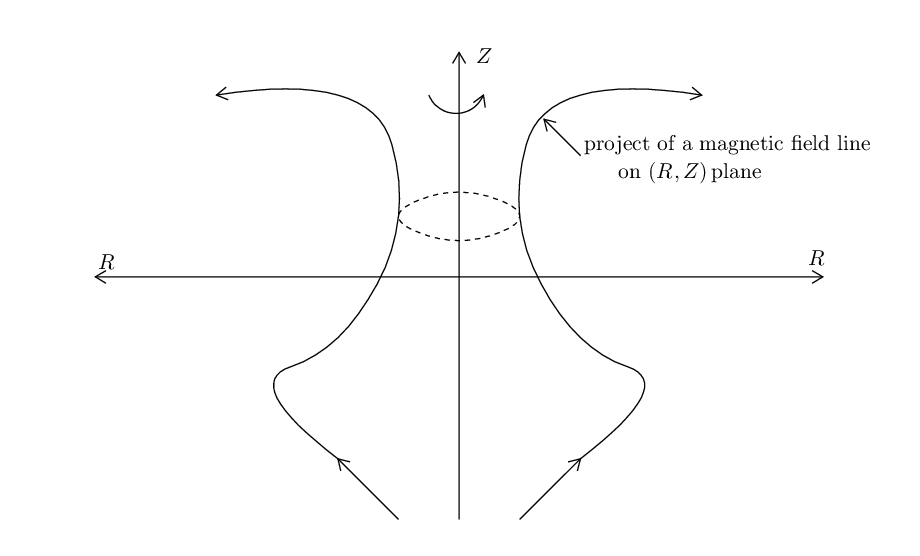
\includegraphics{/home/yj/theory/tokamak_equilibrium/figures/axisymmetrical_magnetic_field-1b.eps}%
\lthtmlpictureZ
\lthtmlcheckvsize\clearpage}

\stepcounter{subsection}
{\newpage\clearpage
\lthtmlinlinemathA{tex2html_wrap_indisplay16888}%
$\displaystyle d \Psi = 0,$%
\lthtmlindisplaymathZ
\lthtmlcheckvsize\clearpage}

{\newpage\clearpage
\lthtmlinlinemathA{tex2html_wrap_indisplay16890}%
$\displaystyle \frac{\partial \Psi}{\partial R} d R + \frac{\partial \Psi}{\partial Z} d Z   = 0.$%
\lthtmlindisplaymathZ
\lthtmlcheckvsize\clearpage}

{\newpage\clearpage
\lthtmlinlinemathA{tex2html_wrap_indisplay16892}%
$\displaystyle \Rightarrow \frac{1}{R}  \frac{\partial \Psi}{\partial R} d R + \frac{1}{R}    \frac{\partial \Psi}{\partial Z} d Z = 0.$%
\lthtmlindisplaymathZ
\lthtmlcheckvsize\clearpage}

{\newpage\clearpage
\lthtmlinlinemathA{tex2html_wrap_indisplay16894}%
$\displaystyle B_Z d R - B_R d Z = 0,$%
\lthtmlindisplaymathZ
\lthtmlcheckvsize\clearpage}

{\newpage\clearpage
\lthtmlinlinemathA{tex2html_wrap_indisplay16896}%
$\displaystyle \frac{d Z}{d R} = \frac{B_Z}{B_R},$%
\lthtmlindisplaymathZ
\lthtmlcheckvsize\clearpage}

\stepcounter{subsection}
{\newpage\clearpage
\lthtmlinlinemathA{tex2html_wrap_inline16909}%
$ \Psi = R A_{\phi}$%
\lthtmlinlinemathZ
\lthtmlcheckvsize\clearpage}

{\newpage\clearpage
\lthtmlpictureA{tex2html_wrap16935}%
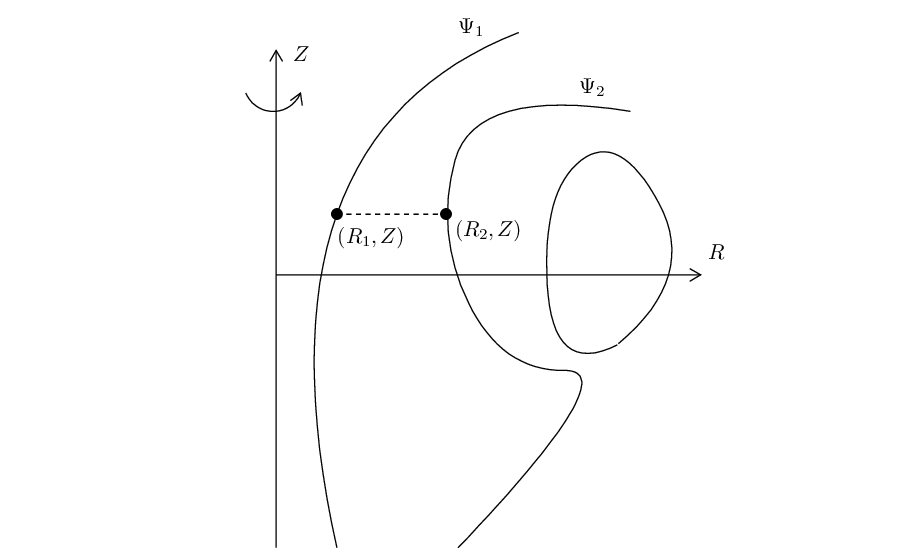
\includegraphics{/home/yj/theory/tokamak_equilibrium/figures/axisymmetrical_magnetic_field-3b.eps}%
\lthtmlpictureZ
\lthtmlcheckvsize\clearpage}

{\newpage\clearpage
\lthtmlinlinemathA{tex2html_wrap_inline16937}%
$ \Psi = \Psi_1$%
\lthtmlinlinemathZ
\lthtmlcheckvsize\clearpage}

{\newpage\clearpage
\lthtmlinlinemathA{tex2html_wrap_inline16939}%
$ \Psi = \Psi_2$%
\lthtmlinlinemathZ
\lthtmlcheckvsize\clearpage}

{\newpage\clearpage
\lthtmlinlinemathA{tex2html_wrap_inline16945}%
$ \hat{\mathbf{Z}}$%
\lthtmlinlinemathZ
\lthtmlcheckvsize\clearpage}

{\newpage\clearpage
\lthtmlinlinemathA{tex2html_wrap_indisplay16948}%
$\displaystyle \Psi_p$%
\lthtmlindisplaymathZ
\lthtmlcheckvsize\clearpage}

{\newpage\clearpage
\lthtmlinlinemathA{tex2html_wrap_indisplay16952}%
$\displaystyle \int_{R_1}^{R_2} B_z (R, Z) 2 \pi R d R$%
\lthtmlindisplaymathZ
\lthtmlcheckvsize\clearpage}

{\newpage\clearpage
\lthtmlinlinemathA{tex2html_wrap_indisplay16956}%
$\displaystyle \int_{R_1}^{R_2} \frac{1}{R}  \frac{\partial \Psi}{\partial R} 2 \pi
R d R$%
\lthtmlindisplaymathZ
\lthtmlcheckvsize\clearpage}

{\newpage\clearpage
\lthtmlinlinemathA{tex2html_wrap_indisplay16960}%
$\displaystyle 2 \pi \int^{R_2}_{R_1} \frac{\partial \Psi}{\partial R} d R$%
\lthtmlindisplaymathZ
\lthtmlcheckvsize\clearpage}

{\newpage\clearpage
\lthtmlinlinemathA{tex2html_wrap_indisplay16964}%
$\displaystyle 2 \pi [\Psi_2 - \Psi_1] .$%
\lthtmlindisplaymathZ
\lthtmlcheckvsize\clearpage}

{\newpage\clearpage
\lthtmlinlinemathA{tex2html_wrap_inline16968}%
$ 2 \pi \Psi$%
\lthtmlinlinemathZ
\lthtmlcheckvsize\clearpage}

\stepcounter{subsection}
{\newpage\clearpage
\lthtmlpictureA{tex2html_wrap17019}%
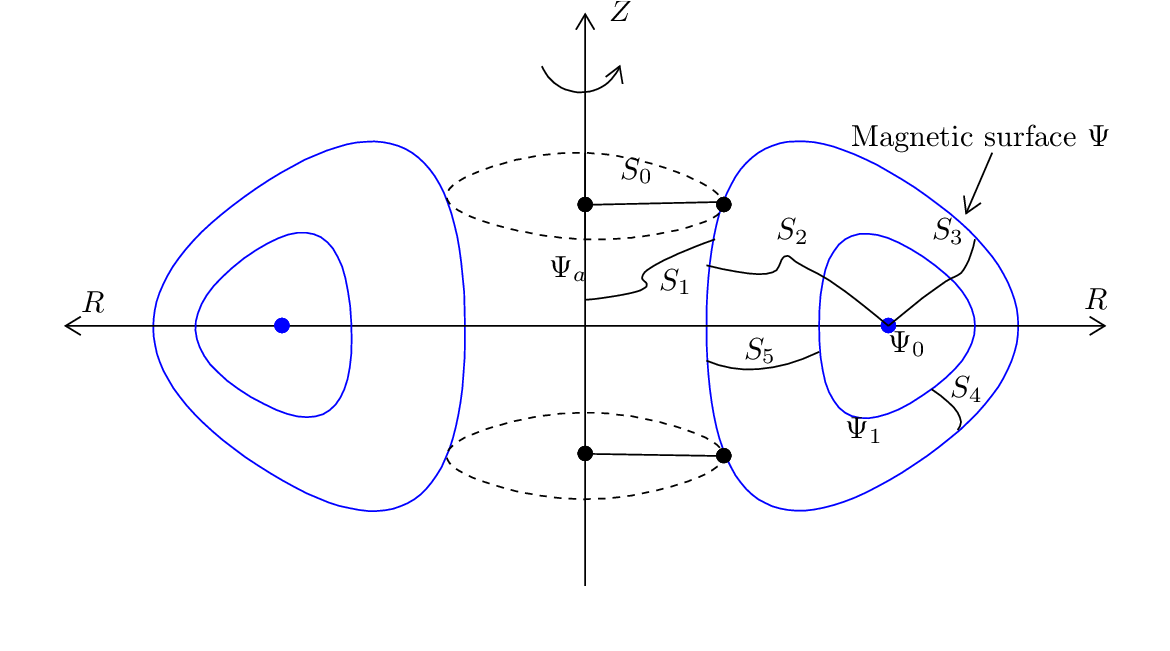
\includegraphics{/home/yj/theory/tokamak_equilibrium/figures/poloidal_flux-1.eps}%
\lthtmlpictureZ
\lthtmlcheckvsize\clearpage}

{\newpage\clearpage
\lthtmlinlinemathA{tex2html_wrap_inline17021}%
$ \Psi_0$%
\lthtmlinlinemathZ
\lthtmlcheckvsize\clearpage}

{\newpage\clearpage
\lthtmlinlinemathA{tex2html_wrap_inline17025}%
$ \nabla \Psi$%
\lthtmlinlinemathZ
\lthtmlcheckvsize\clearpage}

{\newpage\clearpage
\lthtmlinlinemathA{tex2html_wrap_indisplay17031}%
$\displaystyle \Psi_p = 2 \pi (\Psi_0 - \Psi),$%
\lthtmlindisplaymathZ
\lthtmlcheckvsize\clearpage}

{\newpage\clearpage
\lthtmlinlinemathA{tex2html_wrap_indisplay17045}%
$\displaystyle \Psi_p = 2 \pi (\Psi - \Psi_a),$%
\lthtmlindisplaymathZ
\lthtmlcheckvsize\clearpage}

{\newpage\clearpage
\lthtmlinlinemathA{tex2html_wrap_inline17049}%
$ \mathbf{B}_p = \nabla \Psi \times \nabla \phi$%
\lthtmlinlinemathZ
\lthtmlcheckvsize\clearpage}

{\newpage\clearpage
\lthtmlinlinemathA{tex2html_wrap_inline17051}%
$ \Psi_{\ensuremath{\operatorname{LCFS}}} - \Psi_{\ensuremath{\operatorname{axis}}} > 0$%
\lthtmlinlinemathZ
\lthtmlcheckvsize\clearpage}

{\newpage\clearpage
\lthtmlinlinemathA{tex2html_wrap_inline17053}%
$ \mathbf{B}_p$%
\lthtmlinlinemathZ
\lthtmlcheckvsize\clearpage}

{\newpage\clearpage
\lthtmlinlinemathA{tex2html_wrap_inline17055}%
$ \ensuremath{\boldsymbol{\phi}}$%
\lthtmlinlinemathZ
\lthtmlcheckvsize\clearpage}

{\newpage\clearpage
\lthtmlinlinemathA{tex2html_wrap_inline17057}%
$ \Psi_{\ensuremath{\operatorname{LCFS}}} - \Psi_{\ensuremath{\operatorname{axis}}} < 0$%
\lthtmlinlinemathZ
\lthtmlcheckvsize\clearpage}

\stepcounter{subsection}
{\newpage\clearpage
\lthtmlpictureA{tex2html_wrap17096}%
\includegraphics{/home/yj/project_new/solovev_equilibrium/fig2/plt.eps}%
\lthtmlpictureZ
\lthtmlcheckvsize\clearpage}

{\newpage\clearpage
\lthtmlinlinemathA{tex2html_wrap_indisplay17098}%
$\displaystyle R_0 = \frac{R_{\ensuremath{\operatorname{in}}} + R_{\ensuremath{\operatorname{out}}}}{2},$%
\lthtmlindisplaymathZ
\lthtmlcheckvsize\clearpage}

{\newpage\clearpage
\lthtmlinlinemathA{tex2html_wrap_indisplay17102}%
$\displaystyle a = \frac{R_{\ensuremath{\operatorname{out}}} - R_{\ensuremath{\operatorname{in}}}}{2},$%
\lthtmlindisplaymathZ
\lthtmlcheckvsize\clearpage}

{\newpage\clearpage
\lthtmlinlinemathA{tex2html_wrap_indisplay17104}%
$\displaystyle \delta = \frac{R_0 - R_{\ensuremath{\operatorname{top}}}}{a},$%
\lthtmlindisplaymathZ
\lthtmlcheckvsize\clearpage}

{\newpage\clearpage
\lthtmlinlinemathA{tex2html_wrap_indisplay17106}%
$\displaystyle \kappa = \frac{Z_{\ensuremath{\operatorname{top}}}}{a} .$%
\lthtmlindisplaymathZ
\lthtmlcheckvsize\clearpage}

{\newpage\clearpage
\lthtmlinlinemathA{tex2html_wrap_inline17108}%
$ \kappa$%
\lthtmlinlinemathZ
\lthtmlcheckvsize\clearpage}

{\newpage\clearpage
\lthtmlinlinemathA{tex2html_wrap_inline17110}%
$ (\kappa - 1)$%
\lthtmlinlinemathZ
\lthtmlcheckvsize\clearpage}

{\newpage\clearpage
\lthtmlinlinemathA{tex2html_wrap_inline17112}%
$ R_0$%
\lthtmlinlinemathZ
\lthtmlcheckvsize\clearpage}

{\newpage\clearpage
\lthtmlinlinemathA{tex2html_wrap_inline17114}%
$ a$%
\lthtmlinlinemathZ
\lthtmlcheckvsize\clearpage}

{\newpage\clearpage
\lthtmlinlinemathA{tex2html_wrap_inline17116}%
$ \delta$%
\lthtmlinlinemathZ
\lthtmlcheckvsize\clearpage}

{\newpage\clearpage
\lthtmlinlinemathA{tex2html_wrap_inline17120}%
$ (R_{\ensuremath{\operatorname{in}}}, R_{\ensuremath{\operatorname{out}}},
R_{\ensuremath{\operatorname{top}}}, Z_{\ensuremath{\operatorname{top}}})$%
\lthtmlinlinemathZ
\lthtmlcheckvsize\clearpage}

{\newpage\clearpage
\lthtmlinlinemathA{tex2html_wrap_inline17126}%
$ \varepsilon \equiv a / R_0$%
\lthtmlinlinemathZ
\lthtmlcheckvsize\clearpage}

{\newpage\clearpage
\lthtmlinlinemathA{tex2html_wrap_inline17128}%
$ R_0 = 1.85 m$%
\lthtmlinlinemathZ
\lthtmlcheckvsize\clearpage}

{\newpage\clearpage
\lthtmlinlinemathA{tex2html_wrap_inline17130}%
$ 1.9 m$%
\lthtmlinlinemathZ
\lthtmlcheckvsize\clearpage}

{\newpage\clearpage
\lthtmlinlinemathA{tex2html_wrap_inline17132}%
$ a = 0.45 m$%
\lthtmlinlinemathZ
\lthtmlcheckvsize\clearpage}

{\newpage\clearpage
\lthtmlinlinemathA{tex2html_wrap_inline17134}%
$ \kappa = 1.8$%
\lthtmlinlinemathZ
\lthtmlcheckvsize\clearpage}

{\newpage\clearpage
\lthtmlinlinemathA{tex2html_wrap_inline17140}%
$ R_{\ensuremath{\operatorname{axis}}}$%
\lthtmlinlinemathZ
\lthtmlcheckvsize\clearpage}

{\newpage\clearpage
\lthtmlinlinemathA{tex2html_wrap_inline17144}%
$ R_{\ensuremath{\operatorname{axis}}} > R_0$%
\lthtmlinlinemathZ
\lthtmlcheckvsize\clearpage}

\stepcounter{subsection}
\stepcounter{subsubsection}
{\newpage\clearpage
\lthtmlinlinemathA{tex2html_wrap_inline17148}%
$ q$%
\lthtmlinlinemathZ
\lthtmlcheckvsize\clearpage}

{\newpage\clearpage
\lthtmlinlinemathA{tex2html_wrap_indisplay17150}%
$\displaystyle q \equiv \frac{\triangle \phi}{2 \pi},$%
\lthtmlindisplaymathZ
\lthtmlcheckvsize\clearpage}

{\newpage\clearpage
\lthtmlinlinemathA{tex2html_wrap_inline17152}%
$ \triangle \phi$%
\lthtmlinlinemathZ
\lthtmlcheckvsize\clearpage}

\stepcounter{subsubsection}
{\newpage\clearpage
\lthtmlinlinemathA{tex2html_wrap_indisplay17155}%
$\displaystyle \frac{R d \phi}{d \ell_p} = \frac{B_{\phi}}{B_p},$%
\lthtmlindisplaymathZ
\lthtmlcheckvsize\clearpage}

{\newpage\clearpage
\lthtmlinlinemathA{tex2html_wrap_inline17157}%
$ d \ell_p$%
\lthtmlinlinemathZ
\lthtmlcheckvsize\clearpage}

{\newpage\clearpage
\lthtmlinlinemathA{tex2html_wrap_indisplay17161}%
$\displaystyle d \phi = \frac{1}{R} \frac{B_{\phi}}{B_p} d \ell_p,$%
\lthtmlindisplaymathZ
\lthtmlcheckvsize\clearpage}

{\newpage\clearpage
\lthtmlinlinemathA{tex2html_wrap_indisplay17165}%
$\displaystyle \triangle \phi = \oint \frac{1}{R}  \frac{B_{\phi}}{B_p} d \ell_p,$%
\lthtmlindisplaymathZ
\lthtmlcheckvsize\clearpage}

{\newpage\clearpage
\lthtmlinlinemathA{tex2html_wrap_indisplay17169}%
$\displaystyle q = \frac{1}{2 \pi} \oint \frac{1}{R}  \frac{B_{\phi}}{B_p} d   \ell_p .$%
\lthtmlindisplaymathZ
\lthtmlcheckvsize\clearpage}

\stepcounter{subsubsection}
{\newpage\clearpage
\lthtmlinlinemathA{tex2html_wrap_inline17172}%
$ d \Psi_p$%
\lthtmlinlinemathZ
\lthtmlcheckvsize\clearpage}

{\newpage\clearpage
\lthtmlinlinemathA{tex2html_wrap_indisplay17176}%
$\displaystyle d \Psi_p = 2 \pi R d x B_p$%
\lthtmlindisplaymathZ
\lthtmlcheckvsize\clearpage}

{\newpage\clearpage
\lthtmlinlinemathA{tex2html_wrap_inline17178}%
$ d x$%
\lthtmlinlinemathZ
\lthtmlcheckvsize\clearpage}

{\newpage\clearpage
\lthtmlinlinemathA{tex2html_wrap_indisplay17182}%
$\displaystyle B_p = \frac{1}{2 \pi R}  \frac{d \Psi_p}{d x} .$%
\lthtmlindisplaymathZ
\lthtmlcheckvsize\clearpage}

{\newpage\clearpage
\lthtmlinlinemathA{tex2html_wrap_indisplay17184}%
$\displaystyle q = \frac{1}{2 \pi} \oint \frac{1}{R} \frac{B_{\phi}}{B_p} d \ell_p =   \frac{1}{2 \pi} \oint \frac{1}{R} \frac{2 \pi R d x B_{\phi}}{d \Psi_p} d   \ell_p = \oint \frac{d x B_{\phi}}{d \Psi_p} d \ell_p .$%
\lthtmlindisplaymathZ
\lthtmlcheckvsize\clearpage}

{\newpage\clearpage
\lthtmlinlinemathA{tex2html_wrap_indisplay17190}%
$\displaystyle q = \frac{1}{d \Psi_p} \oint d x B_{\phi} d \ell_p$%
\lthtmlindisplaymathZ
\lthtmlcheckvsize\clearpage}

{\newpage\clearpage
\lthtmlinlinemathA{tex2html_wrap_inline17192}%
$ d \Psi_t$%
\lthtmlinlinemathZ
\lthtmlcheckvsize\clearpage}

{\newpage\clearpage
\lthtmlinlinemathA{tex2html_wrap_indisplay17194}%
$\displaystyle d \Psi_t = \oint (B_{\phi} d x) d \ell_p$%
\lthtmlindisplaymathZ
\lthtmlcheckvsize\clearpage}

{\newpage\clearpage
\lthtmlinlinemathA{tex2html_wrap_indisplay17196}%
$\displaystyle q = \frac{d \Psi_t}{d \Psi_p}$%
\lthtmlindisplaymathZ
\lthtmlcheckvsize\clearpage}

\stepcounter{subsubsection}
{\newpage\clearpage
\lthtmlinlinemathA{tex2html_wrap_inline17199}%
$ q = n
/ m$%
\lthtmlinlinemathZ
\lthtmlcheckvsize\clearpage}

{\newpage\clearpage
\lthtmlinlinemathA{tex2html_wrap_inline17201}%
$ m$%
\lthtmlinlinemathZ
\lthtmlcheckvsize\clearpage}

{\newpage\clearpage
\lthtmlinlinemathA{tex2html_wrap_inline17203}%
$ n$%
\lthtmlinlinemathZ
\lthtmlcheckvsize\clearpage}

{\newpage\clearpage
\lthtmlpictureA{tex2html_wrap17221}%
\includegraphics{/home/yj/project_new/nbi_fig/fig12/p.eps}%
\lthtmlpictureZ
\lthtmlcheckvsize\clearpage}

{\newpage\clearpage
\lthtmlpictureA{tex2html_wrap17222}%
\includegraphics{/home/yj/project_new/nbi_fig/fig12b/p.eps}%
\lthtmlpictureZ
\lthtmlcheckvsize\clearpage}

\stepcounter{subsection}
{\newpage\clearpage
\lthtmlinlinemathA{tex2html_wrap_indisplay17225}%
$\displaystyle \mu_0 \mathbf{J}= \nabla \times \mathbf{B}= - \frac{\partial   B_{\phi}}{\partial Z} \hat{\mathbf{R}} + \frac{1}{R} \frac{\partial (R   B_{\phi})}{\partial R} \hat{\mathbf{Z}} + \left( \frac{\partial   B_R}{\partial Z} - \frac{\partial B_Z}{\partial R} \right)   \hat{\ensuremath{\boldsymbol{\phi}}} .$%
\lthtmlindisplaymathZ
\lthtmlcheckvsize\clearpage}

\stepcounter{subsubsection}
{\newpage\clearpage
\lthtmlinlinemathA{tex2html_wrap_inline17228}%
$ g \equiv R B_{\phi}$%
\lthtmlinlinemathZ
\lthtmlcheckvsize\clearpage}

{\newpage\clearpage
\lthtmlinlinemathA{tex2html_wrap_inline17230}%
$ J_Z$%
\lthtmlinlinemathZ
\lthtmlcheckvsize\clearpage}

{\newpage\clearpage
\lthtmlinlinemathA{tex2html_wrap_inline17232}%
$ J_R$%
\lthtmlinlinemathZ
\lthtmlcheckvsize\clearpage}

{\newpage\clearpage
\lthtmlinlinemathA{tex2html_wrap_indisplay17234}%
$\displaystyle \mu_0 J_R = - \frac{1}{R} \frac{\partial g}{\partial Z},$%
\lthtmlindisplaymathZ
\lthtmlcheckvsize\clearpage}

{\newpage\clearpage
\lthtmlinlinemathA{tex2html_wrap_indisplay17236}%
$\displaystyle \mu_0 J_Z = \frac{1}{R} \frac{\partial g}{\partial R},$%
\lthtmlindisplaymathZ
\lthtmlcheckvsize\clearpage}

\stepcounter{subsubsection}
{\newpage\clearpage
\lthtmlinlinemathA{tex2html_wrap_inline17239}%
$ J_{\phi}$%
\lthtmlinlinemathZ
\lthtmlcheckvsize\clearpage}

{\newpage\clearpage
\lthtmlinlinemathA{tex2html_wrap_indisplay17242}%
$\displaystyle \mu_0 J_{\phi}$%
\lthtmlindisplaymathZ
\lthtmlcheckvsize\clearpage}

{\newpage\clearpage
\lthtmlinlinemathA{tex2html_wrap_indisplay17246}%
$\displaystyle \frac{\partial B_R}{\partial Z} - \frac{\partial
B_Z}{\partial R}$%
\lthtmlindisplaymathZ
\lthtmlcheckvsize\clearpage}

{\newpage\clearpage
\lthtmlinlinemathA{tex2html_wrap_indisplay17250}%
$\displaystyle - \frac{1}{R} \frac{\partial^2 \Psi}{\partial Z^2} -
\frac{\partial}{\partial R} \left( \frac{1}{R} \frac{\partial \Psi}{\partial
R} \right)$%
\lthtmlindisplaymathZ
\lthtmlcheckvsize\clearpage}

{\newpage\clearpage
\lthtmlinlinemathA{tex2html_wrap_indisplay17252}%
$\displaystyle \triangle^{\ast} \Psi \equiv \frac{\partial^2}{\partial Z^2} + R   \frac{\partial}{\partial R} \left( \frac{1}{R} \frac{\partial \Psi}{\partial   R} \right),$%
\lthtmlindisplaymathZ
\lthtmlcheckvsize\clearpage}

{\newpage\clearpage
\lthtmlinlinemathA{tex2html_wrap_indisplay17254}%
$\displaystyle \mu_0 J_{\phi} = - \frac{1}{R} \triangle^{\ast} \Psi .$%
\lthtmlindisplaymathZ
\lthtmlcheckvsize\clearpage}

\stepcounter{section}
\stepcounter{subsection}
{\newpage\clearpage
\lthtmlinlinemathA{tex2html_wrap_indisplay17258}%
$\displaystyle \rho \left( \frac{\partial \mathbf{u}}{\partial t} +\mathbf{u} \cdot \nabla   \mathbf{u} \right) = \rho_q \mathbf{E}- \nabla \cdot \mathbbm{P}+\mathbf{J}   \times \mathbf{B},$%
\lthtmlindisplaymathZ
\lthtmlcheckvsize\clearpage}

{\newpage\clearpage
\lthtmlinlinemathA{tex2html_wrap_inline17260}%
$ \rho$%
\lthtmlinlinemathZ
\lthtmlcheckvsize\clearpage}

{\newpage\clearpage
\lthtmlinlinemathA{tex2html_wrap_inline17262}%
$ \rho_q$%
\lthtmlinlinemathZ
\lthtmlcheckvsize\clearpage}

{\newpage\clearpage
\lthtmlinlinemathA{tex2html_wrap_inline17264}%
$ \mathbbm{P}$%
\lthtmlinlinemathZ
\lthtmlcheckvsize\clearpage}

{\newpage\clearpage
\lthtmlinlinemathA{tex2html_wrap_inline17266}%
$ \mathbf{J}$%
\lthtmlinlinemathZ
\lthtmlcheckvsize\clearpage}

{\newpage\clearpage
\lthtmlinlinemathA{tex2html_wrap_inline17268}%
$ \mathbf{E}$%
\lthtmlinlinemathZ
\lthtmlcheckvsize\clearpage}

{\newpage\clearpage
\lthtmlinlinemathA{tex2html_wrap_inline17272}%
$ \rho_q \mathbf{E}$%
\lthtmlinlinemathZ
\lthtmlcheckvsize\clearpage}

{\newpage\clearpage
\lthtmlinlinemathA{tex2html_wrap_inline17274}%
$ \rho_q = 0$%
\lthtmlinlinemathZ
\lthtmlcheckvsize\clearpage}

{\newpage\clearpage
\lthtmlinlinemathA{tex2html_wrap_inline17276}%
$ \mathbf{E}= 0$%
\lthtmlinlinemathZ
\lthtmlcheckvsize\clearpage}

{\newpage\clearpage
\lthtmlinlinemathA{tex2html_wrap_indisplay17278}%
$\displaystyle \mathbf{J} \times \mathbf{B}= \nabla P,$%
\lthtmlindisplaymathZ
\lthtmlcheckvsize\clearpage}

{\newpage\clearpage
\lthtmlinlinemathA{tex2html_wrap_inline17280}%
$ P$%
\lthtmlinlinemathZ
\lthtmlcheckvsize\clearpage}

\stepcounter{subsubsection}
{\newpage\clearpage
\lthtmlinlinemathA{tex2html_wrap_indisplay17287}%
$\displaystyle 0 =\mathbf{B} \cdot \nabla P,$%
\lthtmlindisplaymathZ
\lthtmlcheckvsize\clearpage}

{\newpage\clearpage
\lthtmlinlinemathA{tex2html_wrap_inline17301}%
$ P = P (\Psi)$%
\lthtmlinlinemathZ
\lthtmlcheckvsize\clearpage}

{\newpage\clearpage
\lthtmlinlinemathA{tex2html_wrap_inline17307}%
$ \mathbf{B} \cdot \nabla P =
0$%
\lthtmlinlinemathZ
\lthtmlcheckvsize\clearpage}

{\newpage\clearpage
\lthtmlinlinemathA{tex2html_wrap_indisplay17321}%
$\displaystyle \mathbf{B} \cdot \nabla P = \frac{d P}{d \Psi} \mathbf{B} \cdot \nabla \Psi
   = 0, $%
\lthtmlindisplaymathZ
\lthtmlcheckvsize\clearpage}

\stepcounter{subsubsection}
{\newpage\clearpage
\lthtmlinlinemathA{tex2html_wrap_indisplay17328}%
$\displaystyle J_Z B_R - J_R B_Z = \frac{1}{R} \frac{\partial   P}{\partial \phi} .$%
\lthtmlindisplaymathZ
\lthtmlcheckvsize\clearpage}

{\newpage\clearpage
\lthtmlinlinemathA{tex2html_wrap_inline17332}%
$ \partial P / \partial \phi = 0$%
\lthtmlinlinemathZ
\lthtmlcheckvsize\clearpage}

{\newpage\clearpage
\lthtmlinlinemathA{tex2html_wrap_indisplay17334}%
$\displaystyle J_Z B_R - J_R B_Z = 0$%
\lthtmlindisplaymathZ
\lthtmlcheckvsize\clearpage}

{\newpage\clearpage
\lthtmlinlinemathA{tex2html_wrap_indisplay17336}%
$\displaystyle \frac{\partial g}{\partial R} B_R + \frac{\partial   g}{\partial Z} B_Z = 0,$%
\lthtmlindisplaymathZ
\lthtmlcheckvsize\clearpage}

{\newpage\clearpage
\lthtmlinlinemathA{tex2html_wrap_indisplay17338}%
$\displaystyle \mathbf{B} \cdot \nabla g = 0.$%
\lthtmlindisplaymathZ
\lthtmlcheckvsize\clearpage}

{\newpage\clearpage
\lthtmlinlinemathA{tex2html_wrap_inline17340}%
$ g = g (\Psi)$%
\lthtmlinlinemathZ
\lthtmlcheckvsize\clearpage}

\stepcounter{subsubsection}
{\newpage\clearpage
\lthtmlinlinemathA{tex2html_wrap_inline17345}%
$ \hat{\mathbf{R}}$%
\lthtmlinlinemathZ
\lthtmlcheckvsize\clearpage}

{\newpage\clearpage
\lthtmlinlinemathA{tex2html_wrap_indisplay17349}%
$\displaystyle J_{\phi} B_Z - J_Z B_{\phi} = \frac{\partial P}{\partial   R}$%
\lthtmlindisplaymathZ
\lthtmlcheckvsize\clearpage}

{\newpage\clearpage
\lthtmlinlinemathA{tex2html_wrap_indisplay17351}%
$\displaystyle - \frac{1}{R} \triangle^{\ast} \Psi \frac{1}{R}   \frac{\partial \Psi}{\partial R} - \frac{1}{R} \frac{\partial g}{\partial R}   \frac{g}{R} = \mu_0 \frac{\partial P}{\partial R} .$%
\lthtmlindisplaymathZ
\lthtmlcheckvsize\clearpage}

{\newpage\clearpage
\lthtmlinlinemathA{tex2html_wrap_indisplay17363}%
$\displaystyle - \frac{1}{R} \triangle^{\ast} \Psi \frac{1}{R} \frac{\partial   \Psi}{\partial R} - \frac{1}{R} \frac{d g}{d \Psi} \frac{\partial   \Psi}{\partial R}  \frac{g}{R} = \mu_0 \frac{d P}{d \Psi} \frac{\partial   \Psi}{\partial R},$%
\lthtmlindisplaymathZ
\lthtmlcheckvsize\clearpage}

{\newpage\clearpage
\lthtmlinlinemathA{tex2html_wrap_indisplay17365}%
$\displaystyle \triangle^{\ast} \Psi = - \mu_0 R^2 \frac{d P}{d \Psi} - \frac{d g}{d \Psi}   g,$%
\lthtmlindisplaymathZ
\lthtmlcheckvsize\clearpage}

{\newpage\clearpage
\lthtmlinlinemathA{tex2html_wrap_indisplay17367}%
$\displaystyle \frac{\partial^2 \Psi}{\partial Z^2} + R   \frac{\partial}{\partial R} \left( \frac{1}{R} \frac{\partial \Psi}{\partial   R} \right) = - \mu_0 R^2 \frac{d P}{d \Psi} - \frac{d g}{d \Psi} g.$%
\lthtmlindisplaymathZ
\lthtmlcheckvsize\clearpage}

{\newpage\clearpage
\lthtmlinlinemathA{tex2html_wrap_indisplay17371}%
$\displaystyle \begin{array}{l}
     J_R B_{\phi} - J_{\phi} B_R = \frac{\partial P}{\partial Z}\\
     \Rightarrow - \frac{\partial g}{\partial Z} \frac{1}{R} \frac{g}{R} -
     \frac{1}{R} \triangle^{\ast} \psi \frac{1}{R} \frac{\partial
     \Psi}{\partial Z} = \mu_0 \frac{d P}{d \Psi} \frac{\partial
     \Psi}{\partial Z}\\
     \Rightarrow - \frac{d g}{d \Psi} \frac{\partial \Psi}{\partial Z}
     \frac{1}{R} \frac{g}{R} - \frac{1}{R} \triangle^{\ast} \Psi \frac{1}{R}
     \frac{\partial \Psi}{\partial Z} = \mu_0 \frac{d P}{d \Psi}
     \frac{\partial \Psi}{\partial Z}\\
     \Rightarrow - \frac{d g}{d \Psi} \frac{1}{R} \frac{g}{R} - \frac{1}{R}
     \triangle^{\ast} \Psi \frac{1}{R} = \mu_0 \frac{d P}{d \Psi}\\
     \Rightarrow \triangle^{\ast} \Psi = - \mu_0 R^2 \frac{d P}{d \Psi} -
     \frac{d g}{d \Psi} g
   \end{array} $%
\lthtmlindisplaymathZ
\lthtmlcheckvsize\clearpage}

\stepcounter{subsection}
{\newpage\clearpage
\lthtmlinlinemathA{tex2html_wrap_indisplay17380}%
$\displaystyle \mathbf{B}= \nabla \Psi \times \nabla \phi + g \nabla \phi,$%
\lthtmlindisplaymathZ
\lthtmlcheckvsize\clearpage}

{\newpage\clearpage
\lthtmlinlinemathA{tex2html_wrap_inline17392}%
$ \Psi = \Psi (R, Z)$%
\lthtmlinlinemathZ
\lthtmlcheckvsize\clearpage}

{\newpage\clearpage
\lthtmlinlinemathA{tex2html_wrap_inline17398}%
$ P (\Psi)$%
\lthtmlinlinemathZ
\lthtmlcheckvsize\clearpage}

{\newpage\clearpage
\lthtmlinlinemathA{tex2html_wrap_inline17400}%
$ g (\Psi)$%
\lthtmlinlinemathZ
\lthtmlcheckvsize\clearpage}

{\newpage\clearpage
\lthtmlinlinemathA{tex2html_wrap_indisplay17412}%
$\displaystyle \mathbf{B}_p = \nabla \Psi \times \nabla \phi,$%
\lthtmlindisplaymathZ
\lthtmlcheckvsize\clearpage}

{\newpage\clearpage
\lthtmlinlinemathA{tex2html_wrap_indisplay17414}%
$\displaystyle \mathbf{B}_{\phi} = g \nabla \phi,$%
\lthtmlindisplaymathZ
\lthtmlcheckvsize\clearpage}

\stepcounter{subsection}
{\newpage\clearpage
\lthtmlinlinemathA{tex2html_wrap_indisplay17423}%
$\displaystyle \mu_0 J_R = - \frac{1}{R} \frac{\partial g}{\partial \Psi}  \frac{\partial   \Psi}{\partial Z} = \frac{\partial g}{\partial \Psi} B_R,$%
\lthtmlindisplaymathZ
\lthtmlcheckvsize\clearpage}

{\newpage\clearpage
\lthtmlinlinemathA{tex2html_wrap_indisplay17425}%
$\displaystyle \mu_0 J_Z = \frac{1}{R} \frac{\partial g}{\partial \Psi}  \frac{\partial   \Psi}{\partial R} = \frac{\partial g}{\partial \Psi} B_z,$%
\lthtmlindisplaymathZ
\lthtmlcheckvsize\clearpage}

{\newpage\clearpage
\lthtmlinlinemathA{tex2html_wrap_indisplay17427}%
$\displaystyle \frac{J_R}{J_Z} = \frac{B_R}{B_Z},$%
\lthtmlindisplaymathZ
\lthtmlcheckvsize\clearpage}

{\newpage\clearpage
\lthtmlinlinemathA{tex2html_wrap_inline17435}%
$ \nabla \cdot \mathbf{J}= 0$%
\lthtmlinlinemathZ
\lthtmlcheckvsize\clearpage}

{\newpage\clearpage
\lthtmlinlinemathA{tex2html_wrap_indisplay17437}%
$\displaystyle I_{\ensuremath{\operatorname{pol}}} = \frac{1}{\mu_0} 2 \pi [g (\Psi_2) - g   (\Psi_1)],$%
\lthtmlindisplaymathZ
\lthtmlcheckvsize\clearpage}

{\newpage\clearpage
\lthtmlinlinemathA{tex2html_wrap_inline17439}%
$ I_{\ensuremath{\operatorname{pol}}}$%
\lthtmlinlinemathZ
\lthtmlcheckvsize\clearpage}

{\newpage\clearpage
\lthtmlinlinemathA{tex2html_wrap_indisplay17453}%
$\displaystyle \left\{ \begin{array}{l}
     \mathbf{B}= \nabla \times \mathbf{A}\\
     \Psi = R A_{\phi}
   \end{array} \right. $%
\lthtmlindisplaymathZ
\lthtmlcheckvsize\clearpage}

{\newpage\clearpage
\lthtmlinlinemathA{tex2html_wrap_indisplay17455}%
$\displaystyle \left\{ \begin{array}{l}
     \mu_0 \mathbf{J}= \nabla \times \mathbf{B}\\
     g = R B_{\phi}
   \end{array} \right. $%
\lthtmlindisplaymathZ
\lthtmlcheckvsize\clearpage}

\stepcounter{subsection}
{\newpage\clearpage
\lthtmlinlinemathA{tex2html_wrap_inline17458}%
$ \mathbf{R}$%
\lthtmlinlinemathZ
\lthtmlcheckvsize\clearpage}

{\newpage\clearpage
\lthtmlinlinemathA{tex2html_wrap_indisplay17463}%
$\displaystyle J_{\phi}$%
\lthtmlindisplaymathZ
\lthtmlcheckvsize\clearpage}

{\newpage\clearpage
\lthtmlinlinemathA{tex2html_wrap_indisplay17467}%
$\displaystyle - \frac{1}{\mu_0 R} \triangle^{\ast} \Psi$%
\lthtmlindisplaymathZ
\lthtmlcheckvsize\clearpage}

{\newpage\clearpage
\lthtmlinlinemathA{tex2html_wrap_indisplay17471}%
$\displaystyle R \frac{d P}{d \Psi} + \frac{1}{\mu_0 R}  \frac{d g}{d \Psi} g.$%
\lthtmlindisplaymathZ
\lthtmlcheckvsize\clearpage}

{\newpage\clearpage
\lthtmlinlinemathA{tex2html_wrap_inline17473}%
$ \mathbf{J}_p$%
\lthtmlinlinemathZ
\lthtmlcheckvsize\clearpage}

{\newpage\clearpage
\lthtmlinlinemathA{tex2html_wrap_indisplay17476}%
$\displaystyle \mathbf{J}_p$%
\lthtmlindisplaymathZ
\lthtmlcheckvsize\clearpage}

{\newpage\clearpage
\lthtmlinlinemathA{tex2html_wrap_indisplay17478}%
$\displaystyle \equiv$%
\lthtmlindisplaymathZ
\lthtmlcheckvsize\clearpage}

{\newpage\clearpage
\lthtmlinlinemathA{tex2html_wrap_indisplay17480}%
$\displaystyle J_R \hat{\mathbf{R}} + J_Z \hat{\mathbf{Z}}$%
\lthtmlindisplaymathZ
\lthtmlcheckvsize\clearpage}

{\newpage\clearpage
\lthtmlinlinemathA{tex2html_wrap_indisplay17484}%
$\displaystyle \frac{1}{\mu_0} \left( - \frac{1}{R}  \frac{\partial g}{\partial Z}
\hat{\mathbf{R}} + \frac{1}{R} \frac{\partial g}{\partial R}
\hat{\mathbf{Z}} \right) .$%
\lthtmlindisplaymathZ
\lthtmlcheckvsize\clearpage}

{\newpage\clearpage
\lthtmlinlinemathA{tex2html_wrap_indisplay17488}%
$\displaystyle \frac{1}{\mu_0} \nabla g \times \nabla \phi$%
\lthtmlindisplaymathZ
\lthtmlcheckvsize\clearpage}

{\newpage\clearpage
\lthtmlinlinemathA{tex2html_wrap_indisplay17497}%
$\displaystyle \frac{1}{\mu_0}  \frac{d g}{d \Psi} \nabla \Psi \times
\nabla \phi$%
\lthtmlindisplaymathZ
\lthtmlcheckvsize\clearpage}

{\newpage\clearpage
\lthtmlinlinemathA{tex2html_wrap_indisplay17501}%
$\displaystyle \frac{1}{\mu_0}  \frac{d g}{d \Psi} \mathbf{B}_p .$%
\lthtmlindisplaymathZ
\lthtmlcheckvsize\clearpage}

{\newpage\clearpage
\lthtmlinlinemathA{tex2html_wrap_indisplay17504}%
$\displaystyle J_{\parallel}$%
\lthtmlindisplaymathZ
\lthtmlcheckvsize\clearpage}

{\newpage\clearpage
\lthtmlinlinemathA{tex2html_wrap_indisplay17508}%
$\displaystyle \frac{\mathbf{J} \cdot \mathbf{B}}{B}$%
\lthtmlindisplaymathZ
\lthtmlcheckvsize\clearpage}

{\newpage\clearpage
\lthtmlinlinemathA{tex2html_wrap_indisplay17512}%
$\displaystyle \frac{J_{\phi} B_{\phi} +\mathbf{J}_p \cdot \mathbf{B}_p}{B}$%
\lthtmlindisplaymathZ
\lthtmlcheckvsize\clearpage}

{\newpage\clearpage
\lthtmlinlinemathA{tex2html_wrap_indisplay17516}%
$\displaystyle \frac{\left( R \frac{d P}{d \Psi} + \frac{1}{\mu_0 R}  \frac{d g}{d
\Psi} g \right) \frac{g}{R} + \frac{1}{\mu_0}  \frac{d g}{d \Psi} \left(
\frac{\nabla \Psi}{R} \right)^2}{B}$%
\lthtmlindisplaymathZ
\lthtmlcheckvsize\clearpage}

{\newpage\clearpage
\lthtmlinlinemathA{tex2html_wrap_indisplay17520}%
$\displaystyle \frac{g \frac{d P}{d \Psi} + \frac{1}{\mu_0}  \frac{d g}{d \Psi}
\left[  \left( \frac{g}{R} \right)^2 + \left( \frac{\nabla \Psi}{R}
\right)^2 \right]}{B}$%
\lthtmlindisplaymathZ
\lthtmlcheckvsize\clearpage}

{\newpage\clearpage
\lthtmlinlinemathA{tex2html_wrap_indisplay17524}%
$\displaystyle \frac{g \frac{d P}{d \Psi} + \frac{1}{\mu_0}  \frac{d g}{d \Psi}
B^2}{B} .$%
\lthtmlindisplaymathZ
\lthtmlcheckvsize\clearpage}

{\newpage\clearpage
\lthtmlinlinemathA{tex2html_wrap_indisplay17527}%
$\displaystyle \sigma$%
\lthtmlindisplaymathZ
\lthtmlcheckvsize\clearpage}

{\newpage\clearpage
\lthtmlinlinemathA{tex2html_wrap_indisplay17531}%
$\displaystyle \frac{J_{\parallel}}{B}$%
\lthtmlindisplaymathZ
\lthtmlcheckvsize\clearpage}

{\newpage\clearpage
\lthtmlinlinemathA{tex2html_wrap_indisplay17535}%
$\displaystyle g \frac{d P}{d \Psi}  \frac{1}{B^2} + \frac{1}{\mu_0}  \frac{d g}{d
\Psi} .$%
\lthtmlindisplaymathZ
\lthtmlcheckvsize\clearpage}

{\newpage\clearpage
\lthtmlinlinemathA{tex2html_wrap_inline17537}%
$ J_{\parallel} / B$%
\lthtmlinlinemathZ
\lthtmlcheckvsize\clearpage}

{\newpage\clearpage
\lthtmlinlinemathA{tex2html_wrap_inline17539}%
$ \mu_0 J_{\parallel} / B$%
\lthtmlinlinemathZ
\lthtmlcheckvsize\clearpage}

{\newpage\clearpage
\lthtmlinlinemathA{tex2html_wrap_inline17543}%
$ \sigma_{\ensuremath{\operatorname{ps}}}$%
\lthtmlinlinemathZ
\lthtmlcheckvsize\clearpage}

{\newpage\clearpage
\lthtmlinlinemathA{tex2html_wrap_indisplay17546}%
$\displaystyle \sigma_{\ensuremath{\operatorname{ps}}}$%
\lthtmlindisplaymathZ
\lthtmlcheckvsize\clearpage}

{\newpage\clearpage
\lthtmlinlinemathA{tex2html_wrap_indisplay17550}%
$\displaystyle \sigma - \langle \sigma \rangle$%
\lthtmlindisplaymathZ
\lthtmlcheckvsize\clearpage}

{\newpage\clearpage
\lthtmlinlinemathA{tex2html_wrap_indisplay17554}%
$\displaystyle g \frac{d P}{d \Psi} \left[  \frac{1}{B^2} - \left\langle
\frac{1}{B^2} \right\rangle \right]$%
\lthtmlindisplaymathZ
\lthtmlcheckvsize\clearpage}

{\newpage\clearpage
\lthtmlinlinemathA{tex2html_wrap_indisplay17558}%
$\displaystyle \frac{J_{\parallel}^{\ensuremath{\operatorname{ps}}}}{B},$%
\lthtmlindisplaymathZ
\lthtmlcheckvsize\clearpage}

{\newpage\clearpage
\lthtmlinlinemathA{tex2html_wrap_inline17560}%
$ J_{\parallel}^{\ensuremath{\operatorname{ps}}}$%
\lthtmlinlinemathZ
\lthtmlcheckvsize\clearpage}

{\newpage\clearpage
\lthtmlinlinemathA{tex2html_wrap_inline17562}%
$ \mu_0 \langle \mathbf{J} \cdot \mathbf{B}
\rangle$%
\lthtmlinlinemathZ
\lthtmlcheckvsize\clearpage}

{\newpage\clearpage
\lthtmlinlinemathA{tex2html_wrap_indisplay17565}%
$\displaystyle \mu_0 \langle \mathbf{J} \cdot \mathbf{B} \rangle$%
\lthtmlindisplaymathZ
\lthtmlcheckvsize\clearpage}

{\newpage\clearpage
\lthtmlinlinemathA{tex2html_wrap_indisplay17569}%
$\displaystyle \mu_0 g \frac{d P}{d
\Psi} + \frac{d g}{d \Psi} \langle B^2 \rangle,$%
\lthtmlindisplaymathZ
\lthtmlcheckvsize\clearpage}

{\newpage\clearpage
\lthtmlinlinemathA{tex2html_wrap_inline17571}%
$ \langle \ldots \rangle$%
\lthtmlinlinemathZ
\lthtmlcheckvsize\clearpage}

\stepcounter{subsection}
{\newpage\clearpage
\lthtmlinlinemathA{tex2html_wrap_indisplay17582}%
$\displaystyle \frac{d P}{d \Psi} = - \frac{c_1}{\mu_0},$%
\lthtmlindisplaymathZ
\lthtmlcheckvsize\clearpage}

{\newpage\clearpage
\lthtmlinlinemathA{tex2html_wrap_indisplay17584}%
$\displaystyle g \frac{d g}{d \Psi} = - c_2 R_0^2,$%
\lthtmlindisplaymathZ
\lthtmlcheckvsize\clearpage}

{\newpage\clearpage
\lthtmlinlinemathA{tex2html_wrap_indisplay17586}%
$\displaystyle \Psi = \frac{1}{2} (c_2 R_0^2 + c_0 R^2) Z^2 + \frac{1}{8}   (c_1 - c_0) (R^2 - R_0^2)^2,$%
\lthtmlindisplaymathZ
\lthtmlcheckvsize\clearpage}

{\newpage\clearpage
\lthtmlinlinemathA{tex2html_wrap_inline17588}%
$ c_0$%
\lthtmlinlinemathZ
\lthtmlcheckvsize\clearpage}

{\newpage\clearpage
\lthtmlinlinemathA{tex2html_wrap_inline17590}%
$ c_1$%
\lthtmlinlinemathZ
\lthtmlcheckvsize\clearpage}

{\newpage\clearpage
\lthtmlinlinemathA{tex2html_wrap_inline17592}%
$ c_2$%
\lthtmlinlinemathZ
\lthtmlcheckvsize\clearpage}

{\newpage\clearpage
\lthtmlinlinemathA{tex2html_wrap_inline17598}%
$ c_0 = B_0 / (R_0^2 \kappa_0 q_0)$%
\lthtmlinlinemathZ
\lthtmlcheckvsize\clearpage}

{\newpage\clearpage
\lthtmlinlinemathA{tex2html_wrap_inline17600}%
$ c_1 = B_0 (\kappa_0^2 + 1) / (R_0^2
\kappa_0 q_0)$%
\lthtmlinlinemathZ
\lthtmlcheckvsize\clearpage}

{\newpage\clearpage
\lthtmlinlinemathA{tex2html_wrap_inline17602}%
$ c_2 = 0$%
\lthtmlinlinemathZ
\lthtmlcheckvsize\clearpage}

{\newpage\clearpage
\lthtmlinlinemathA{tex2html_wrap_indisplay17604}%
$\displaystyle \Psi = \frac{B_0}{2 R_0^2 \kappa_0 q_0} \left[ R^2 Z^2 +   \frac{\kappa_0^2}{4} (R^2 - R_0^2)^2 \right],$%
\lthtmlindisplaymathZ
\lthtmlcheckvsize\clearpage}

{\newpage\clearpage
\lthtmlinlinemathA{tex2html_wrap_indisplay17610}%
$\displaystyle Z = \pm \frac{1}{R} \sqrt{\frac{2 R_0^2 \kappa_0 q_0}{B_0}   \Psi - \frac{\kappa_0^2}{4} (R^2 - R_0^2)^2},$%
\lthtmlindisplaymathZ
\lthtmlcheckvsize\clearpage}

{\newpage\clearpage
\lthtmlinlinemathA{tex2html_wrap_indisplay17612}%
$\displaystyle \frac{d P}{d \Psi} = - \frac{c_1}{\mu_0} = - \frac{B_0 (\kappa_0^2 +   1)}{\mu_0 R_0^2 \kappa_0 q_0},$%
\lthtmlindisplaymathZ
\lthtmlcheckvsize\clearpage}

{\newpage\clearpage
\lthtmlinlinemathA{tex2html_wrap_indisplay17614}%
$\displaystyle P = P_0 - \frac{B_0 (\kappa_0^2 + 1)}{\mu_0 R_0^2 \kappa_0   q_0} \Psi,$%
\lthtmlindisplaymathZ
\lthtmlcheckvsize\clearpage}

{\newpage\clearpage
\lthtmlinlinemathA{tex2html_wrap_inline17618}%
$ \Psi = 0$%
\lthtmlinlinemathZ
\lthtmlcheckvsize\clearpage}

{\newpage\clearpage
\lthtmlinlinemathA{tex2html_wrap_inline17620}%
$ R = R_0, Z = 0$%
\lthtmlinlinemathZ
\lthtmlcheckvsize\clearpage}

{\newpage\clearpage
\lthtmlinlinemathA{tex2html_wrap_inline17628}%
$ q_0 g / (R_0 B_0)$%
\lthtmlinlinemathZ
\lthtmlcheckvsize\clearpage}

{\newpage\clearpage
\lthtmlinlinemathA{tex2html_wrap_indisplay17633}%
$\displaystyle | \nabla \Psi |$%
\lthtmlindisplaymathZ
\lthtmlcheckvsize\clearpage}

{\newpage\clearpage
\lthtmlinlinemathA{tex2html_wrap_indisplay17637}%
$\displaystyle \sqrt{\left( \frac{\partial \Psi}{\partial R}
\right)^2 + \left( \frac{\partial \Psi}{\partial Z} \right)^2}$%
\lthtmlindisplaymathZ
\lthtmlcheckvsize\clearpage}

{\newpage\clearpage
\lthtmlinlinemathA{tex2html_wrap_indisplay17641}%
$\displaystyle \frac{B_0}{2 R_0^2 \kappa_0 q_0} \sqrt{[2 R Z^2 + \kappa_0^2 (R^2 -
R_0^2) R]^2 + (2 R^2 Z)^2} .$%
\lthtmlindisplaymathZ
\lthtmlcheckvsize\clearpage}

{\newpage\clearpage
\lthtmlinlinemathA{tex2html_wrap_inline17643}%
$ \Psi_0 = B_0 R_0^2$%
\lthtmlinlinemathZ
\lthtmlcheckvsize\clearpage}

{\newpage\clearpage
\lthtmlinlinemathA{tex2html_wrap_inline17645}%
$ \overline{\Psi} = \Psi / \Psi_0$%
\lthtmlinlinemathZ
\lthtmlcheckvsize\clearpage}

{\newpage\clearpage
\lthtmlinlinemathA{tex2html_wrap_indisplay17648}%
$\displaystyle \overline{\Psi}$%
\lthtmlindisplaymathZ
\lthtmlcheckvsize\clearpage}

{\newpage\clearpage
\lthtmlinlinemathA{tex2html_wrap_indisplay17652}%
$\displaystyle \frac{1}{2 \kappa_0 q_0} \left[ \overline{R}^2
\overline{Z}^2 + \frac{\kappa_0^2}{4} (\overline{R}^2 - 1)^2 \right],$%
\lthtmlindisplaymathZ
\lthtmlcheckvsize\clearpage}

{\newpage\clearpage
\lthtmlinlinemathA{tex2html_wrap_inline17654}%
$ \overline{R} = R / R_0$%
\lthtmlinlinemathZ
\lthtmlcheckvsize\clearpage}

{\newpage\clearpage
\lthtmlinlinemathA{tex2html_wrap_inline17656}%
$ \overline{Z} = Z / R_0$%
\lthtmlinlinemathZ
\lthtmlcheckvsize\clearpage}

{\newpage\clearpage
\lthtmlinlinemathA{tex2html_wrap_indisplay17658}%
$\displaystyle \overline{Z} = \pm \frac{1}{\overline{R}} \sqrt{2 \kappa_0   q_0 \overline{\Psi} - \frac{\kappa_0^2}{4} (\overline{R}^2 - 1)^2} .$%
\lthtmlindisplaymathZ
\lthtmlcheckvsize\clearpage}

{\newpage\clearpage
\lthtmlinlinemathA{tex2html_wrap_inline17660}%
$ \kappa_0$%
\lthtmlinlinemathZ
\lthtmlcheckvsize\clearpage}

{\newpage\clearpage
\lthtmlinlinemathA{tex2html_wrap_inline17662}%
$ q_0$%
\lthtmlinlinemathZ
\lthtmlcheckvsize\clearpage}

{\newpage\clearpage
\lthtmlinlinemathA{tex2html_wrap_inline17666}%
$ (\overline{R}, \overline{Z})$%
\lthtmlinlinemathZ
\lthtmlcheckvsize\clearpage}

{\newpage\clearpage
\lthtmlpictureA{tex2html_wrap17710}%
\includegraphics{/home/yj/project_new/solovev_equilibrium/fig1/plt.eps}%
\lthtmlpictureZ
\lthtmlcheckvsize\clearpage}

{\newpage\clearpage
\lthtmlinlinemathA{tex2html_wrap_indisplay17712}%
$\displaystyle R_{\ensuremath{\operatorname{in}}} = \sqrt{R_0^2 - \sqrt{A \Psi}},$%
\lthtmlindisplaymathZ
\lthtmlcheckvsize\clearpage}

{\newpage\clearpage
\lthtmlinlinemathA{tex2html_wrap_indisplay17714}%
$\displaystyle R_{\ensuremath{\operatorname{out}}} = \sqrt{R_0^2 + \sqrt{A \Psi}},$%
\lthtmlindisplaymathZ
\lthtmlcheckvsize\clearpage}

{\newpage\clearpage
\lthtmlinlinemathA{tex2html_wrap_indisplay17716}%
$\displaystyle a = \frac{R_{\ensuremath{\operatorname{out}}} - R_{\ensuremath{\operatorname{in}}}}{2} =   \frac{\sqrt{R_0^2 + \sqrt{A \Psi}} - \sqrt{R_0^2 - \sqrt{A \Psi}}}{2} .$%
\lthtmlindisplaymathZ
\lthtmlcheckvsize\clearpage}

{\newpage\clearpage
\lthtmlinlinemathA{tex2html_wrap_inline17718}%
$ A = 8 R_0^2 q_0 / (B_0 \kappa_0)$%
\lthtmlinlinemathZ
\lthtmlcheckvsize\clearpage}

{\newpage\clearpage
\lthtmlinlinemathA{tex2html_wrap_inline17726}%
$ R_{\ensuremath{\operatorname{in}}} =
R_{\ensuremath{\operatorname{out}}} = R_0$%
\lthtmlinlinemathZ
\lthtmlcheckvsize\clearpage}

{\newpage\clearpage
\lthtmlinlinemathA{tex2html_wrap_inline17728}%
$ \Psi = R_0^2
B_0 \kappa_0 / (8 q_0)$%
\lthtmlinlinemathZ
\lthtmlcheckvsize\clearpage}

{\newpage\clearpage
\lthtmlinlinemathA{tex2html_wrap_inline17730}%
$ R_{\ensuremath{\operatorname{in}}} = 0$%
\lthtmlinlinemathZ
\lthtmlcheckvsize\clearpage}

{\newpage\clearpage
\lthtmlinlinemathA{tex2html_wrap_inline17734}%
$ 0
\leqslant \Psi < R_0^2 B_0 \kappa_0 / (8 q_0)$%
\lthtmlinlinemathZ
\lthtmlcheckvsize\clearpage}

{\newpage\clearpage
\lthtmlinlinemathA{tex2html_wrap_indisplay17738}%
$\displaystyle \varepsilon \approx \sqrt{\frac{2 q_0 \Psi}{\kappa_0 R_0^2 B_0}} .$%
\lthtmlindisplaymathZ
\lthtmlcheckvsize\clearpage}

{\newpage\clearpage
\lthtmlinlinemathA{tex2html_wrap_indisplay17744}%
$\displaystyle \Psi = \frac{\varepsilon^2 \kappa_0 R_0^2 B_0}{2 q_0} .$%
\lthtmlindisplaymathZ
\lthtmlcheckvsize\clearpage}

\stepcounter{subsection}
{\newpage\clearpage
\lthtmlinlinemathA{tex2html_wrap_inline17755}%
$ \Psi_2 = s \Psi$%
\lthtmlinlinemathZ
\lthtmlcheckvsize\clearpage}

{\newpage\clearpage
\lthtmlinlinemathA{tex2html_wrap_inline17757}%
$ P_2 =
s^2 P (\Psi)$%
\lthtmlinlinemathZ
\lthtmlcheckvsize\clearpage}

{\newpage\clearpage
\lthtmlinlinemathA{tex2html_wrap_inline17759}%
$ g_2 = \pm s g (\Psi)$%
\lthtmlinlinemathZ
\lthtmlcheckvsize\clearpage}

{\newpage\clearpage
\lthtmlinlinemathA{tex2html_wrap_inline17761}%
$ s$%
\lthtmlinlinemathZ
\lthtmlcheckvsize\clearpage}

{\newpage\clearpage
\lthtmlinlinemathA{tex2html_wrap_inline17765}%
$ s^2$%
\lthtmlinlinemathZ
\lthtmlcheckvsize\clearpage}

{\newpage\clearpage
\lthtmlinlinemathA{tex2html_wrap_inline17767}%
$ \beta$%
\lthtmlinlinemathZ
\lthtmlcheckvsize\clearpage}

{\newpage\clearpage
\lthtmlinlinemathA{tex2html_wrap_inline17775}%
$ \Psi_2 = \Psi$%
\lthtmlinlinemathZ
\lthtmlcheckvsize\clearpage}

{\newpage\clearpage
\lthtmlinlinemathA{tex2html_wrap_inline17777}%
$ P_2 = P (\Psi)$%
\lthtmlinlinemathZ
\lthtmlcheckvsize\clearpage}

{\newpage\clearpage
\lthtmlinlinemathA{tex2html_wrap_inline17779}%
$ g^2_2 = g^2 (\Psi) + c$%
\lthtmlinlinemathZ
\lthtmlcheckvsize\clearpage}

{\newpage\clearpage
\lthtmlinlinemathA{tex2html_wrap_inline17781}%
$ g_2 g_2' = g g'$%
\lthtmlinlinemathZ
\lthtmlcheckvsize\clearpage}

{\newpage\clearpage
\lthtmlinlinemathA{tex2html_wrap_inline17783}%
$ \beta_p$%
\lthtmlinlinemathZ
\lthtmlcheckvsize\clearpage}

{\newpage\clearpage
\lthtmlinlinemathA{tex2html_wrap_inline17787}%
$ P_2 = P (\Psi)
+ c$%
\lthtmlinlinemathZ
\lthtmlcheckvsize\clearpage}

{\newpage\clearpage
\lthtmlinlinemathA{tex2html_wrap_inline17789}%
$ g_2 = g (\Psi)$%
\lthtmlinlinemathZ
\lthtmlcheckvsize\clearpage}

\stepcounter{subsection}
{\newpage\clearpage
\lthtmlinlinemathA{tex2html_wrap_inline17792}%
$ \nabla P \approx P_0 / a$%
\lthtmlinlinemathZ
\lthtmlcheckvsize\clearpage}

{\newpage\clearpage
\lthtmlinlinemathA{tex2html_wrap_inline17798}%
$ P_0 \approx 2 \times 10^4
\ensuremath{\operatorname{Pa}}$%
\lthtmlinlinemathZ
\lthtmlcheckvsize\clearpage}

{\newpage\clearpage
\lthtmlinlinemathA{tex2html_wrap_inline17802}%
$ \nabla P \approx P_0 / a = 4 \times 10^4 N /
m^3$%
\lthtmlinlinemathZ
\lthtmlcheckvsize\clearpage}

{\newpage\clearpage
\lthtmlinlinemathA{tex2html_wrap_indisplay17804}%
$\displaystyle F_{\ensuremath{\operatorname{rot}}} = \rho_m U^2 / R \approx 4 \times 10^{19} m^{- 3} \times
   1.67 \times 10^{- 27} \ensuremath{\operatorname{kg}} U^2 / 1.85 = 3.6 \times 10^{- 8} U^2, $%
\lthtmlindisplaymathZ
\lthtmlcheckvsize\clearpage}

{\newpage\clearpage
\lthtmlinlinemathA{tex2html_wrap_inline17806}%
$ U$%
\lthtmlinlinemathZ
\lthtmlcheckvsize\clearpage}

{\newpage\clearpage
\lthtmlinlinemathA{tex2html_wrap_inline17808}%
$ \nabla P$%
\lthtmlinlinemathZ
\lthtmlcheckvsize\clearpage}

{\newpage\clearpage
\lthtmlinlinemathA{tex2html_wrap_indisplay17810}%
$\displaystyle 3.6 \times 10^{- 8} U^2 = 4 \times 10^4, $%
\lthtmlindisplaymathZ
\lthtmlcheckvsize\clearpage}

{\newpage\clearpage
\lthtmlinlinemathA{tex2html_wrap_inline17812}%
$ U \approx 1.0 \times 10^6 m /
s$%
\lthtmlinlinemathZ
\lthtmlcheckvsize\clearpage}

{\newpage\clearpage
\lthtmlinlinemathA{tex2html_wrap_inline17814}%
$ f = U / (2 \pi R) = 86
\ensuremath{\operatorname{KHz}}$%
\lthtmlinlinemathZ
\lthtmlcheckvsize\clearpage}

{\newpage\clearpage
\lthtmlinlinemathA{tex2html_wrap_inline17816}%
$ \ensuremath{\operatorname{KHz}}$%
\lthtmlinlinemathZ
\lthtmlcheckvsize\clearpage}

{\newpage\clearpage
\lthtmlinlinemathA{tex2html_wrap_indisplay17818}%
$\displaystyle \rho_m \left[ \frac{\partial \mathbf{U}}{\partial t} +\mathbf{U} \cdot   \nabla \mathbf{U} \right] = \rho_q \mathbf{E}+\mathbf{J} \times \mathbf{B}-   \nabla \cdot \mathbbm{P},$%
\lthtmlindisplaymathZ
\lthtmlcheckvsize\clearpage}

{\newpage\clearpage
\lthtmlinlinemathA{tex2html_wrap_inline17822}%
$ \rho_q
\approx 0$%
\lthtmlinlinemathZ
\lthtmlcheckvsize\clearpage}

{\newpage\clearpage
\lthtmlinlinemathA{tex2html_wrap_inline17824}%
$ \mathbf{E} \approx 0$%
\lthtmlinlinemathZ
\lthtmlcheckvsize\clearpage}

{\newpage\clearpage
\lthtmlinlinemathA{tex2html_wrap_inline17828}%
$ \rho_m = n_D m_D = 4 \times 10^{19} m^{-
3} \times 2 \times 1.6726 \times 10^{- 27} k g = 1.3 \times 10^{- 7} k g /
m^3$%
\lthtmlinlinemathZ
\lthtmlcheckvsize\clearpage}

{\newpage\clearpage
\lthtmlinlinemathA{tex2html_wrap_indisplay17830}%
$\displaystyle \nabla p \approx p_0 / a = 2 \times 10^4 \ensuremath{\operatorname{Pa}} / 0.45 m = 4 \times 10^4   N / m^3$%
\lthtmlindisplaymathZ
\lthtmlcheckvsize\clearpage}

\stepcounter{subsection}
{\newpage\clearpage
\lthtmlinlinemathA{tex2html_wrap_indisplay17835}%
$\displaystyle \beta = \frac{p}{B^2 / 2 \mu_0} .$%
\lthtmlindisplaymathZ
\lthtmlcheckvsize\clearpage}

{\newpage\clearpage
\lthtmlinlinemathA{tex2html_wrap_inline17837}%
$ \beta_t$%
\lthtmlinlinemathZ
\lthtmlcheckvsize\clearpage}

{\newpage\clearpage
\lthtmlinlinemathA{tex2html_wrap_indisplay17841}%
$\displaystyle \beta_t = \frac{\langle p \rangle}{B^2_{t 0} / 2 \mu_0},$%
\lthtmlindisplaymathZ
\lthtmlcheckvsize\clearpage}

{\newpage\clearpage
\lthtmlinlinemathA{tex2html_wrap_indisplay17843}%
$\displaystyle \beta_p = \frac{\langle p \rangle}{B^2_{p a} / 2 \mu_0},$%
\lthtmlindisplaymathZ
\lthtmlcheckvsize\clearpage}

{\newpage\clearpage
\lthtmlinlinemathA{tex2html_wrap_inline17847}%
$ B_{t 0}$%
\lthtmlinlinemathZ
\lthtmlcheckvsize\clearpage}

{\newpage\clearpage
\lthtmlinlinemathA{tex2html_wrap_inline17849}%
$ B_{p a}$%
\lthtmlinlinemathZ
\lthtmlcheckvsize\clearpage}

{\newpage\clearpage
\lthtmlinlinemathA{tex2html_wrap_inline17861}%
$ B_{p a}
\approx \mu_0 I_p / (2 \pi a)$%
\lthtmlinlinemathZ
\lthtmlcheckvsize\clearpage}

{\newpage\clearpage
\lthtmlinlinemathA{tex2html_wrap_indisplay17865}%
$\displaystyle \beta_p \approx \frac{\langle p \rangle}{I_p^2 / (8 \pi^2   a^2)},$%
\lthtmlindisplaymathZ
\lthtmlcheckvsize\clearpage}

{\newpage\clearpage
\lthtmlinlinemathA{tex2html_wrap_inline17869}%
$ \beta_N$%
\lthtmlinlinemathZ
\lthtmlcheckvsize\clearpage}

\stepcounter{subsection}
{\newpage\clearpage
\lthtmlinlinemathA{tex2html_wrap_inline17876}%
$ I_p
/ (a B_{t 0})$%
\lthtmlinlinemathZ
\lthtmlcheckvsize\clearpage}

{\newpage\clearpage
\lthtmlinlinemathA{tex2html_wrap_inline17878}%
$ I_p [\ensuremath{\operatorname{MA}}] / a B_{t 0} \leqslant 3$%
\lthtmlinlinemathZ
\lthtmlcheckvsize\clearpage}

{\newpage\clearpage
\lthtmlinlinemathA{tex2html_wrap_inline17880}%
$ I_p
[\ensuremath{\operatorname{MA}}]$%
\lthtmlinlinemathZ
\lthtmlcheckvsize\clearpage}

{\newpage\clearpage
\lthtmlinlinemathA{tex2html_wrap_inline17886}%
$ \beta_{t \max} \propto I_p / (a B_{t 0})$%
\lthtmlinlinemathZ
\lthtmlcheckvsize\clearpage}

{\newpage\clearpage
\lthtmlinlinemathA{tex2html_wrap_indisplay17890}%
$\displaystyle \beta_N = 10^8 \frac{a B_{t 0}}{I_p} \beta_t,$%
\lthtmlindisplaymathZ
\lthtmlcheckvsize\clearpage}

{\newpage\clearpage
\lthtmlinlinemathA{tex2html_wrap_indisplay17892}%
$\displaystyle \beta_N = 10^8 \frac{\langle p \rangle}{I_p / a},$%
\lthtmlindisplaymathZ
\lthtmlcheckvsize\clearpage}

{\newpage\clearpage
\lthtmlinlinemathA{tex2html_wrap_inline17900}%
$ \beta_N = 7.2$%
\lthtmlinlinemathZ
\lthtmlcheckvsize\clearpage}

{\newpage\clearpage
\lthtmlinlinemathA{tex2html_wrap_inline17904}%
$ \beta_N \geqslant 2$%
\lthtmlinlinemathZ
\lthtmlcheckvsize\clearpage}

{\newpage\clearpage
\lthtmlinlinemathA{tex2html_wrap_inline17908}%
$ I_p$%
\lthtmlinlinemathZ
\lthtmlcheckvsize\clearpage}

{\newpage\clearpage
\lthtmlinlinemathA{tex2html_wrap_inline17922}%
$ \langle p \rangle \propto I_p^{\alpha}$%
\lthtmlinlinemathZ
\lthtmlcheckvsize\clearpage}

{\newpage\clearpage
\lthtmlinlinemathA{tex2html_wrap_inline17924}%
$ 1 < \alpha < 2$%
\lthtmlinlinemathZ
\lthtmlcheckvsize\clearpage}

{\newpage\clearpage
\lthtmlinlinemathA{tex2html_wrap_inline17928}%
$ B_t$%
\lthtmlinlinemathZ
\lthtmlcheckvsize\clearpage}

\stepcounter{subsection}
{\newpage\clearpage
\lthtmlinlinemathA{tex2html_wrap_inline17935}%
$ I_p / a B_{t
0}$%
\lthtmlinlinemathZ
\lthtmlcheckvsize\clearpage}

{\newpage\clearpage
\lthtmlinlinemathA{tex2html_wrap_inline17937}%
$ I_p
/ a$%
\lthtmlinlinemathZ
\lthtmlcheckvsize\clearpage}

{\newpage\clearpage
\lthtmlinlinemathA{tex2html_wrap_indisplay17939}%
$\displaystyle \langle p \rangle \propto \frac{I_p}{a}$%
\lthtmlindisplaymathZ
\lthtmlcheckvsize\clearpage}

{\newpage\clearpage
\lthtmlinlinemathA{tex2html_wrap_inline17941}%
$ E \approx \langle p \rangle 2 \pi R a^2$%
\lthtmlinlinemathZ
\lthtmlcheckvsize\clearpage}

{\newpage\clearpage
\lthtmlinlinemathA{tex2html_wrap_indisplay17945}%
$\displaystyle E \propto I_p a R.$%
\lthtmlindisplaymathZ
\lthtmlcheckvsize\clearpage}

{\newpage\clearpage
\lthtmlinlinemathA{tex2html_wrap_indisplay17947}%
$\displaystyle P_{\ensuremath{\operatorname{fusion}}} \propto I_p a R,$%
\lthtmlindisplaymathZ
\lthtmlcheckvsize\clearpage}

\stepcounter{subsection}
{\newpage\clearpage
\lthtmlinlinemathA{tex2html_wrap_indisplay17950}%
$\displaystyle n_e \approx 1.5 n_G,$%
\lthtmlindisplaymathZ
\lthtmlcheckvsize\clearpage}

{\newpage\clearpage
\lthtmlinlinemathA{tex2html_wrap_inline17952}%
$ n_G$%
\lthtmlinlinemathZ
\lthtmlcheckvsize\clearpage}

{\newpage\clearpage
\lthtmlinlinemathA{tex2html_wrap_indisplay17954}%
$\displaystyle n_G = 10^{20} \frac{I_p}{\pi a^2} \times 10^{- 6}$%
\lthtmlindisplaymathZ
\lthtmlcheckvsize\clearpage}

{\newpage\clearpage
\lthtmlinlinemathA{tex2html_wrap_inline17960}%
$ 1.5 n_G$%
\lthtmlinlinemathZ
\lthtmlcheckvsize\clearpage}

{\newpage\clearpage
\lthtmlinlinemathA{tex2html_wrap_inline17966}%
$ n_e = 1.6 n_G$%
\lthtmlinlinemathZ
\lthtmlcheckvsize\clearpage}

\stepcounter{section}
{\newpage\clearpage
\lthtmlinlinemathA{tex2html_wrap_indisplay17977}%
$\displaystyle \Psi (R', Z') = \int_P G (R, Z ; R', Z') J_{\phi} d R d Z +   \sum_{i = 1}^{N_c} G (R^c_i, Z_i^c ; R', Z') I_{\phi} .$%
\lthtmlindisplaymathZ
\lthtmlcheckvsize\clearpage}

{\newpage\clearpage
\lthtmlinlinemathA{tex2html_wrap_indisplay17981}%
$\displaystyle J_{\phi} = - \frac{1}{\mu_0 R} \triangle^{\ast} \Psi .$%
\lthtmlindisplaymathZ
\lthtmlcheckvsize\clearpage}

{\newpage\clearpage
\lthtmlinlinemathA{tex2html_wrap_inline17995}%
$ \Psi_b$%
\lthtmlinlinemathZ
\lthtmlcheckvsize\clearpage}

{\newpage\clearpage
\lthtmlinlinemathA{tex2html_wrap_inline18015}%
$ (\theta, \zeta)$%
\lthtmlinlinemathZ
\lthtmlcheckvsize\clearpage}

\stepcounter{section}
\stepcounter{subsection}
{\newpage\clearpage
\lthtmlinlinemathA{tex2html_wrap_inline18019}%
$ (x, y,
z)$%
\lthtmlinlinemathZ
\lthtmlcheckvsize\clearpage}

{\newpage\clearpage
\lthtmlinlinemathA{tex2html_wrap_indisplay18021}%
$\displaystyle \mathbf{r}= x \hat{\mathbf{x}} + y \hat{\mathbf{y}} + z \hat{\mathbf{z}},$%
\lthtmlindisplaymathZ
\lthtmlcheckvsize\clearpage}

{\newpage\clearpage
\lthtmlinlinemathA{tex2html_wrap_inline18023}%
$ \mathbf{r}$%
\lthtmlinlinemathZ
\lthtmlcheckvsize\clearpage}

{\newpage\clearpage
\lthtmlinlinemathA{tex2html_wrap_inline18027}%
$ (x^1, x^2, x^3)$%
\lthtmlinlinemathZ
\lthtmlcheckvsize\clearpage}

{\newpage\clearpage
\lthtmlinlinemathA{tex2html_wrap_indisplay18029}%
$\displaystyle \mathbf{r}= x (x^1, x^2, x^3) \hat{\mathbf{x}} + y (x^1,   x^2, x^3) \hat{\mathbf{y}} + z (x^1, x^2, x^3) \hat{\mathbf{z}} .$%
\lthtmlindisplaymathZ
\lthtmlcheckvsize\clearpage}

{\newpage\clearpage
\lthtmlinlinemathA{tex2html_wrap_inline18033}%
$ \mathbf{r}= R \cos \phi
\hat{\mathbf{x}} + R \sin \phi \hat{\mathbf{y}} + Z \hat{\mathbf{z}}$%
\lthtmlinlinemathZ
\lthtmlcheckvsize\clearpage}

{\newpage\clearpage
\lthtmldisplayA{displaymath18035}%
\begin{displaymath}\begin{array}{l}     x = x (x^1, x^2, x^3)\\y = y (x^1, x^2, x^3)\\z = z (x^1, x^2, x^3)   \end{array}\end{displaymath}%
\lthtmldisplayZ
\lthtmlcheckvsize\clearpage}

{\newpage\clearpage
\lthtmlinlinemathA{tex2html_wrap_indisplay18037}%
$\displaystyle \mathcal{J}= \left|\begin{array}{ccc}     \frac{\partial x}{\partial x_1} & \frac{\partial x}{\partial x_2} &     \frac{\partial x}{\partial x_3}\\\frac{\partial y}{\partial x_1} & \frac{\partial y}{\partial x_2} &     \frac{\partial y}{\partial x_3}\\\frac{\partial z}{\partial x_1} & \frac{\partial z}{\partial x_2} &     \frac{\partial z}{\partial x_3}   \end{array}\right|,$%
\lthtmlindisplaymathZ
\lthtmlcheckvsize\clearpage}

{\newpage\clearpage
\lthtmlinlinemathA{tex2html_wrap_indisplay18039}%
$\displaystyle \mathcal{J}= \frac{\partial \mathbf{r}}{\partial x_1}   \times \frac{\partial \mathbf{r}}{\partial x_2} \cdot \frac{\partial   \mathbf{r}}{\partial x_3} .$%
\lthtmlindisplaymathZ
\lthtmlcheckvsize\clearpage}

{\newpage\clearpage
\lthtmlinlinemathA{tex2html_wrap_inline18041}%
$ \mathcal{J}$%
\lthtmlinlinemathZ
\lthtmlcheckvsize\clearpage}

{\newpage\clearpage
\lthtmlinlinemathA{tex2html_wrap_indisplay18043}%
$\displaystyle \mathcal{J}= (\nabla x_1 \times \nabla x_2 \cdot \nabla   x_3)^{- 1} .$%
\lthtmlindisplaymathZ
\lthtmlcheckvsize\clearpage}

\stepcounter{subsection}
{\newpage\clearpage
\lthtmlinlinemathA{tex2html_wrap_indisplay18048}%
$\displaystyle \nabla x^i \cdot \frac{\partial \mathbf{r}}{\partial x^j} =   \delta_{i j},$%
\lthtmlindisplaymathZ
\lthtmlcheckvsize\clearpage}

{\newpage\clearpage
\lthtmlinlinemathA{tex2html_wrap_inline18050}%
$ \delta_{i j}$%
\lthtmlinlinemathZ
\lthtmlcheckvsize\clearpage}

{\newpage\clearpage
\lthtmlinlinemathA{tex2html_wrap_indisplay18053}%
$\displaystyle \nabla x^i \cdot \frac{\partial \mathbf{r}}{\partial x^j}$%
\lthtmlindisplaymathZ
\lthtmlcheckvsize\clearpage}

{\newpage\clearpage
\lthtmlinlinemathA{tex2html_wrap_indisplay18057}%
$\displaystyle \left[
\left( \frac{\partial x^i}{\partial x} \right) \hat{\mathbf{x}} + \left(
\frac{\partial x^i}{\partial y} \right) \hat{\mathbf{y}} + \left(
\frac{\partial x^i}{\partial z} \right) \hat{\mathbf{z}} \right] \cdot
\left[ \frac{\partial x}{\partial x^j} \hat{\mathbf{x}} + x \frac{\partial
\hat{\mathbf{x}}}{\partial x^j} + \frac{\partial y}{\partial x^j}
\hat{\mathbf{y}} + y \frac{\partial \hat{\mathbf{y}}}{\partial x^j} +
\frac{\partial z}{\partial x^j} \hat{\mathbf{z}} + z \frac{\partial
\hat{\mathbf{z}}}{\partial x^j} \right]$%
\lthtmlindisplaymathZ
\lthtmlcheckvsize\clearpage}

{\newpage\clearpage
\lthtmlinlinemathA{tex2html_wrap_indisplay18061}%
$\displaystyle \left[ \left( \frac{\partial x^i}{\partial x} \right)
\hat{\mathbf{x}} + \left( \frac{\partial x^i}{\partial y} \right)
\hat{\mathbf{y}} + \left( \frac{\partial x^i}{\partial z} \right)
\hat{\mathbf{z}} \right] \cdot \left[ \frac{\partial x}{\partial x^j}
\hat{\mathbf{x}} + \frac{\partial y}{\partial x^j} \hat{\mathbf{y}} +
\frac{\partial z}{\partial x^j} \hat{\mathbf{z}} \right]$%
\lthtmlindisplaymathZ
\lthtmlcheckvsize\clearpage}

{\newpage\clearpage
\lthtmlinlinemathA{tex2html_wrap_indisplay18065}%
$\displaystyle \frac{\partial x^i}{\partial x} \frac{\partial x}{\partial x^j} +
\frac{\partial x^i}{\partial y}  \frac{\partial y}{\partial x^j} +
\frac{\partial x^i}{\partial z}  \frac{\partial z}{\partial x^j}$%
\lthtmlindisplaymathZ
\lthtmlcheckvsize\clearpage}

{\newpage\clearpage
\lthtmlinlinemathA{tex2html_wrap_indisplay18069}%
$\displaystyle \frac{\partial x^i}{\partial x^j}$%
\lthtmlindisplaymathZ
\lthtmlcheckvsize\clearpage}

{\newpage\clearpage
\lthtmlinlinemathA{tex2html_wrap_indisplay18073}%
$\displaystyle \delta_{i j},$%
\lthtmlindisplaymathZ
\lthtmlcheckvsize\clearpage}

{\newpage\clearpage
\lthtmlinlinemathA{tex2html_wrap_indisplay18075}%
$\displaystyle \frac{\partial \hat{\mathbf{x}}}{\partial x^j} = 0, \frac{\partial   \hat{\mathbf{y}}}{\partial x^j} = 0, \frac{\partial   \hat{\mathbf{z}}}{\partial x^j} = 0,$%
\lthtmlindisplaymathZ
\lthtmlcheckvsize\clearpage}

{\newpage\clearpage
\lthtmlinlinemathA{tex2html_wrap_inline18077}%
$ \hat{\mathbf{x}}, \hat{\mathbf{y}}, \hat{\mathbf{z}}$%
\lthtmlinlinemathZ
\lthtmlcheckvsize\clearpage}

{\newpage\clearpage
\lthtmlinlinemathA{tex2html_wrap_inline18079}%
$ \nabla x^i$%
\lthtmlinlinemathZ
\lthtmlcheckvsize\clearpage}

{\newpage\clearpage
\lthtmlinlinemathA{tex2html_wrap_inline18081}%
$ \partial
\mathbf{r}/ \partial x^i$%
\lthtmlinlinemathZ
\lthtmlcheckvsize\clearpage}

{\newpage\clearpage
\lthtmlinlinemathA{tex2html_wrap_inline18085}%
$ x = x_1 \cos
x_2$%
\lthtmlinlinemathZ
\lthtmlcheckvsize\clearpage}

{\newpage\clearpage
\lthtmlinlinemathA{tex2html_wrap_inline18087}%
$ y = x_1 \sin x_2$%
\lthtmlinlinemathZ
\lthtmlcheckvsize\clearpage}

{\newpage\clearpage
\lthtmlinlinemathA{tex2html_wrap_inline18089}%
$ z = x_3$%
\lthtmlinlinemathZ
\lthtmlcheckvsize\clearpage}

{\newpage\clearpage
\lthtmlinlinemathA{tex2html_wrap_inline18091}%
$ x_1 \equiv R$%
\lthtmlinlinemathZ
\lthtmlcheckvsize\clearpage}

{\newpage\clearpage
\lthtmlinlinemathA{tex2html_wrap_inline18093}%
$ x_2 \equiv \phi$%
\lthtmlinlinemathZ
\lthtmlcheckvsize\clearpage}

{\newpage\clearpage
\lthtmlinlinemathA{tex2html_wrap_inline18095}%
$ x_3 \equiv Z$%
\lthtmlinlinemathZ
\lthtmlcheckvsize\clearpage}

{\newpage\clearpage
\lthtmlinlinemathA{tex2html_wrap_inline18097}%
$ \partial \mathbf{r}/ \partial
x^1$%
\lthtmlinlinemathZ
\lthtmlcheckvsize\clearpage}

{\newpage\clearpage
\lthtmlinlinemathA{tex2html_wrap_inline18099}%
$ \nabla x^2$%
\lthtmlinlinemathZ
\lthtmlcheckvsize\clearpage}

{\newpage\clearpage
\lthtmlinlinemathA{tex2html_wrap_inline18101}%
$ \nabla x^3$%
\lthtmlinlinemathZ
\lthtmlcheckvsize\clearpage}

{\newpage\clearpage
\lthtmlinlinemathA{tex2html_wrap_indisplay18105}%
$\displaystyle \frac{\partial \mathbf{r}}{\partial x^1} = A \nabla x^2 \times   \nabla x^3,$%
\lthtmlindisplaymathZ
\lthtmlcheckvsize\clearpage}

{\newpage\clearpage
\lthtmlinlinemathA{tex2html_wrap_inline18107}%
$ A$%
\lthtmlinlinemathZ
\lthtmlcheckvsize\clearpage}

{\newpage\clearpage
\lthtmlinlinemathA{tex2html_wrap_inline18111}%
$ \nabla x^1$%
\lthtmlinlinemathZ
\lthtmlcheckvsize\clearpage}

{\newpage\clearpage
\lthtmlinlinemathA{tex2html_wrap_indisplay18113}%
$\displaystyle 1 = A (\nabla x^2 \times \nabla x^3) \cdot \nabla x^1,$%
\lthtmlindisplaymathZ
\lthtmlcheckvsize\clearpage}

{\newpage\clearpage
\lthtmlinlinemathA{tex2html_wrap_indisplay18116}%
$\displaystyle A$%
\lthtmlindisplaymathZ
\lthtmlcheckvsize\clearpage}

{\newpage\clearpage
\lthtmlinlinemathA{tex2html_wrap_indisplay18120}%
$\displaystyle \frac{1}{(\nabla x^2 \times \nabla x^3) \cdot \nabla x^1}$%
\lthtmlindisplaymathZ
\lthtmlcheckvsize\clearpage}

{\newpage\clearpage
\lthtmlinlinemathA{tex2html_wrap_indisplay18124}%
$\displaystyle \mathcal{J}$%
\lthtmlindisplaymathZ
\lthtmlcheckvsize\clearpage}

{\newpage\clearpage
\lthtmlinlinemathA{tex2html_wrap_indisplay18134}%
$\displaystyle \frac{\partial \mathbf{r}}{\partial x^1} =\mathcal{J} \nabla   x^2 \times \nabla x^3 .$%
\lthtmlindisplaymathZ
\lthtmlcheckvsize\clearpage}

{\newpage\clearpage
\lthtmlinlinemathA{tex2html_wrap_indisplay18136}%
$\displaystyle \frac{\partial \mathbf{r}}{\partial x^2} =\mathcal{J} \nabla   x^3 \times \nabla x^1$%
\lthtmlindisplaymathZ
\lthtmlcheckvsize\clearpage}

{\newpage\clearpage
\lthtmlinlinemathA{tex2html_wrap_indisplay18138}%
$\displaystyle \frac{\partial \mathbf{r}}{\partial x^3} =\mathcal{J} \nabla   x^1 \times \nabla x^2 .$%
\lthtmlindisplaymathZ
\lthtmlcheckvsize\clearpage}

{\newpage\clearpage
\lthtmlinlinemathA{tex2html_wrap_indisplay18140}%
$\displaystyle \frac{\partial \mathbf{r}}{\partial x^i} =\mathcal{J} \nabla   x^j \times \nabla x^k,$%
\lthtmlindisplaymathZ
\lthtmlcheckvsize\clearpage}

{\newpage\clearpage
\lthtmlinlinemathA{tex2html_wrap_inline18142}%
$ (i, j, k)$%
\lthtmlinlinemathZ
\lthtmlcheckvsize\clearpage}

{\newpage\clearpage
\lthtmlinlinemathA{tex2html_wrap_indisplay18146}%
$\displaystyle \nabla x^i =\mathcal{J}^{- 1} \frac{\partial \mathbf{r}}{\partial x^j}   \times \frac{\partial \mathbf{r}}{\partial x^k},$%
\lthtmlindisplaymathZ
\lthtmlcheckvsize\clearpage}

\stepcounter{subsection}
{\newpage\clearpage
\lthtmlinlinemathA{tex2html_wrap_inline18153}%
$ \nabla \psi$%
\lthtmlinlinemathZ
\lthtmlcheckvsize\clearpage}

{\newpage\clearpage
\lthtmlinlinemathA{tex2html_wrap_inline18157}%
$ \nabla \zeta$%
\lthtmlinlinemathZ
\lthtmlcheckvsize\clearpage}

{\newpage\clearpage
\lthtmlinlinemathA{tex2html_wrap_indisplay18159}%
$\displaystyle \frac{\partial \mathbf{r}}{\partial \psi} =\mathcal{J} \nabla \theta \times   \nabla \zeta,$%
\lthtmlindisplaymathZ
\lthtmlcheckvsize\clearpage}

{\newpage\clearpage
\lthtmlinlinemathA{tex2html_wrap_indisplay18161}%
$\displaystyle \frac{\partial \mathbf{r}}{\partial \theta} =\mathcal{J} \nabla \zeta \times   \nabla \psi,$%
\lthtmlindisplaymathZ
\lthtmlcheckvsize\clearpage}

{\newpage\clearpage
\lthtmlinlinemathA{tex2html_wrap_indisplay18163}%
$\displaystyle \frac{\partial \mathbf{r}}{\partial \zeta} =\mathcal{J} \nabla \psi \times   \nabla \theta .$%
\lthtmlindisplaymathZ
\lthtmlcheckvsize\clearpage}

{\newpage\clearpage
\lthtmlinlinemathA{tex2html_wrap_indisplay18166}%
$\displaystyle \mathbf{e}^{\psi} \equiv \nabla \psi ;$%
\lthtmlindisplaymathZ
\lthtmlcheckvsize\clearpage}

{\newpage\clearpage
\lthtmlinlinemathA{tex2html_wrap_indisplay18168}%
$\displaystyle \mathbf{e}^{\theta} \equiv \nabla
\theta ;$%
\lthtmlindisplaymathZ
\lthtmlcheckvsize\clearpage}

{\newpage\clearpage
\lthtmlinlinemathA{tex2html_wrap_indisplay18170}%
$\displaystyle \mathbf{e}^{\zeta} \equiv \nabla \zeta .$%
\lthtmlindisplaymathZ
\lthtmlcheckvsize\clearpage}

{\newpage\clearpage
\lthtmlinlinemathA{tex2html_wrap_indisplay18173}%
$\displaystyle \mathbf{e}_{\psi} \equiv \frac{\partial \mathbf{r}}{\partial \psi} ;$%
\lthtmlindisplaymathZ
\lthtmlcheckvsize\clearpage}

{\newpage\clearpage
\lthtmlinlinemathA{tex2html_wrap_indisplay18175}%
$\displaystyle \mathbf{e}_{\theta} \equiv \frac{\partial \mathbf{r}}{\partial \theta} ;$%
\lthtmlindisplaymathZ
\lthtmlcheckvsize\clearpage}

{\newpage\clearpage
\lthtmlinlinemathA{tex2html_wrap_indisplay18177}%
$\displaystyle \mathbf{e}_{\zeta} \equiv \frac{\partial \mathbf{r}}{\partial \zeta} .$%
\lthtmlindisplaymathZ
\lthtmlcheckvsize\clearpage}

{\newpage\clearpage
\lthtmlinlinemathA{tex2html_wrap_indisplay18179}%
$\displaystyle \mathbf{e}^{\alpha} \cdot \mathbf{e}_{\beta} = \delta_{\alpha \beta} .$%
\lthtmlindisplaymathZ
\lthtmlcheckvsize\clearpage}

{\newpage\clearpage
\lthtmlinlinemathA{tex2html_wrap_indisplay18183}%
$\displaystyle \mathbf{A}= A_{\psi} \mathbf{e}^{\psi} + A_{\theta}   \mathbf{e}^{\theta} + A_{\zeta} \mathbf{e}^{\zeta},$%
\lthtmlindisplaymathZ
\lthtmlcheckvsize\clearpage}

{\newpage\clearpage
\lthtmlinlinemathA{tex2html_wrap_inline18185}%
$ A_{\psi} =\mathbf{A} \cdot \mathbf{e}_{\psi}$%
\lthtmlinlinemathZ
\lthtmlcheckvsize\clearpage}

{\newpage\clearpage
\lthtmlinlinemathA{tex2html_wrap_inline18187}%
$ A_{\theta} =\mathbf{A}
\cdot \mathbf{e}_{\theta}$%
\lthtmlinlinemathZ
\lthtmlcheckvsize\clearpage}

{\newpage\clearpage
\lthtmlinlinemathA{tex2html_wrap_inline18189}%
$ A_{\zeta} =\mathbf{A} \cdot
\mathbf{e}_{\zeta}$%
\lthtmlinlinemathZ
\lthtmlcheckvsize\clearpage}

{\newpage\clearpage
\lthtmlinlinemathA{tex2html_wrap_indisplay18193}%
$\displaystyle \mathbf{A}= A^{\psi} \mathbf{e}_{\psi} + A^{\theta}   \mathbf{e}_{\theta} + A^{\zeta} \mathbf{e}_{\zeta},$%
\lthtmlindisplaymathZ
\lthtmlcheckvsize\clearpage}

{\newpage\clearpage
\lthtmlinlinemathA{tex2html_wrap_inline18195}%
$ A^{\psi} =\mathbf{A} \cdot \mathbf{e}^{\psi}$%
\lthtmlinlinemathZ
\lthtmlcheckvsize\clearpage}

{\newpage\clearpage
\lthtmlinlinemathA{tex2html_wrap_inline18197}%
$ A^{\theta} =\mathbf{A}
\cdot \mathbf{e}^{\theta}$%
\lthtmlinlinemathZ
\lthtmlcheckvsize\clearpage}

{\newpage\clearpage
\lthtmlinlinemathA{tex2html_wrap_inline18199}%
$ A^{\zeta} =\mathbf{A} \cdot
\mathbf{e}^{\zeta}$%
\lthtmlinlinemathZ
\lthtmlcheckvsize\clearpage}

{\newpage\clearpage
\lthtmlinlinemathA{tex2html_wrap_inline18201}%
$ \Psi \equiv A_{\phi} R$%
\lthtmlinlinemathZ
\lthtmlcheckvsize\clearpage}

{\newpage\clearpage
\lthtmlinlinemathA{tex2html_wrap_inline18209}%
$ \nabla R$%
\lthtmlinlinemathZ
\lthtmlcheckvsize\clearpage}

{\newpage\clearpage
\lthtmlinlinemathA{tex2html_wrap_inline18211}%
$ \nabla
\phi$%
\lthtmlinlinemathZ
\lthtmlcheckvsize\clearpage}

{\newpage\clearpage
\lthtmlinlinemathA{tex2html_wrap_inline18213}%
$ \nabla Z$%
\lthtmlinlinemathZ
\lthtmlcheckvsize\clearpage}

{\newpage\clearpage
\lthtmlinlinemathA{tex2html_wrap_indisplay18215}%
$\displaystyle \mathbf{A}= A_1 \nabla R + A_2 \nabla \phi + A_3 \nabla Z.$%
\lthtmlindisplaymathZ
\lthtmlcheckvsize\clearpage}

{\newpage\clearpage
\lthtmlinlinemathA{tex2html_wrap_inline18217}%
$ A_2$%
\lthtmlinlinemathZ
\lthtmlcheckvsize\clearpage}

{\newpage\clearpage
\lthtmlinlinemathA{tex2html_wrap_indisplay18225}%
$\displaystyle \mathbf{A} \cdot \frac{\partial \mathbf{r}}{\partial \phi}   = A_2 .$%
\lthtmlindisplaymathZ
\lthtmlcheckvsize\clearpage}

{\newpage\clearpage
\lthtmlinlinemathA{tex2html_wrap_indisplay18229}%
$\displaystyle \mathbf{r} (R, Z, \phi) = R \hat{\mathbf{e}}_R (\phi) + Z \hat{\mathbf{e}}_Z   .$%
\lthtmlindisplaymathZ
\lthtmlcheckvsize\clearpage}

{\newpage\clearpage
\lthtmlinlinemathA{tex2html_wrap_indisplay18231}%
$\displaystyle \frac{\partial \mathbf{r}}{\partial \phi} = R   \hat{\mathbf{e}}_{\phi},$%
\lthtmlindisplaymathZ
\lthtmlcheckvsize\clearpage}

{\newpage\clearpage
\lthtmlinlinemathA{tex2html_wrap_indisplay18233}%
$\displaystyle A_2 = A_{\phi} R,$%
\lthtmlindisplaymathZ
\lthtmlcheckvsize\clearpage}

{\newpage\clearpage
\lthtmlinlinemathA{tex2html_wrap_inline18235}%
$ \Psi = A_{\phi} R$%
\lthtmlinlinemathZ
\lthtmlcheckvsize\clearpage}

\stepcounter{subsection}
{\newpage\clearpage
\lthtmlinlinemathA{tex2html_wrap_inline18240}%
$ f (\psi, \theta, \zeta)$%
\lthtmlinlinemathZ
\lthtmlcheckvsize\clearpage}

{\newpage\clearpage
\lthtmlinlinemathA{tex2html_wrap_indisplay18242}%
$\displaystyle \nabla f = \frac{\partial f}{\partial \psi} \nabla \psi +   \frac{\partial f}{\partial \theta} \nabla \theta + \frac{\partial   f}{\partial \zeta} \nabla \zeta .$%
\lthtmlindisplaymathZ
\lthtmlcheckvsize\clearpage}

{\newpage\clearpage
\lthtmlinlinemathA{tex2html_wrap_indisplay18244}%
$\displaystyle \frac{\partial f}{\partial \psi} = (\mathcal{J} \nabla \theta   \times \nabla \zeta) \cdot \nabla f,$%
\lthtmlindisplaymathZ
\lthtmlcheckvsize\clearpage}

{\newpage\clearpage
\lthtmlinlinemathA{tex2html_wrap_indisplay18246}%
$\displaystyle \frac{\partial f}{\partial \theta} = (\mathcal{J} \nabla \zeta   \times \nabla \psi) \cdot \nabla f,$%
\lthtmlindisplaymathZ
\lthtmlcheckvsize\clearpage}

{\newpage\clearpage
\lthtmlinlinemathA{tex2html_wrap_indisplay18248}%
$\displaystyle \frac{\partial f}{\partial \zeta} = (\mathcal{J} \nabla \psi   \times \nabla \theta) \cdot \nabla f.$%
\lthtmlindisplaymathZ
\lthtmlcheckvsize\clearpage}

{\newpage\clearpage
\lthtmlinlinemathA{tex2html_wrap_indisplay18252}%
$\displaystyle \nabla \psi \cdot \nabla f = | \nabla \psi |^2 \frac{\partial f}{\partial   \psi} + (\nabla \theta \cdot \nabla \psi) \frac{\partial f}{\partial \theta}   + (\nabla \zeta \cdot \nabla \psi) \frac{\partial f}{\partial \zeta} .$%
\lthtmlindisplaymathZ
\lthtmlcheckvsize\clearpage}

\stepcounter{subsection}
{\newpage\clearpage
\lthtmlinlinemathA{tex2html_wrap_indisplay18257}%
$\displaystyle \nabla \cdot (\nabla \alpha \times \nabla \beta) = 0,$%
\lthtmlindisplaymathZ
\lthtmlcheckvsize\clearpage}

{\newpage\clearpage
\lthtmlinlinemathA{tex2html_wrap_indisplay18265}%
$\displaystyle \mathbf{A}= A^1 \mathcal{J} \nabla \theta \times \nabla \zeta + A^2   \mathcal{J} \nabla \zeta \times \nabla \psi + A^3 \mathcal{J} \nabla \psi   \times \nabla \theta,$%
\lthtmlindisplaymathZ
\lthtmlcheckvsize\clearpage}

{\newpage\clearpage
\lthtmlinlinemathA{tex2html_wrap_inline18267}%
$ A^1 =\mathbf{A} \cdot \nabla \psi$%
\lthtmlinlinemathZ
\lthtmlcheckvsize\clearpage}

{\newpage\clearpage
\lthtmlinlinemathA{tex2html_wrap_indisplay18272}%
$\displaystyle \nabla \cdot \mathbf{A}$%
\lthtmlindisplaymathZ
\lthtmlcheckvsize\clearpage}

{\newpage\clearpage
\lthtmlinlinemathA{tex2html_wrap_indisplay18276}%
$\displaystyle \nabla (A^1 \mathcal{J}) \cdot (\nabla \theta
\times \nabla \zeta) + \nabla (A^2 \mathcal{J}) \cdot (\nabla \zeta \times
\nabla \psi) + \nabla (A^3 \mathcal{J}) \cdot (\nabla \psi \times \nabla
\theta)$%
\lthtmlindisplaymathZ
\lthtmlcheckvsize\clearpage}

{\newpage\clearpage
\lthtmlinlinemathA{tex2html_wrap_indisplay18280}%
$\displaystyle \frac{1}{\mathcal{J}} \left( \frac{\partial A^1 \mathcal{J}}{\partial
\psi} + \frac{\partial A^2 \mathcal{J}}{\partial \theta} + \frac{\partial
A^3 \mathcal{J}}{\partial \zeta} \right),$%
\lthtmlindisplaymathZ
\lthtmlcheckvsize\clearpage}

\stepcounter{subsection}
{\newpage\clearpage
\lthtmlinlinemathA{tex2html_wrap_indisplay18288}%
$\displaystyle \nabla f$%
\lthtmlindisplaymathZ
\lthtmlcheckvsize\clearpage}

{\newpage\clearpage
\lthtmlinlinemathA{tex2html_wrap_indisplay18292}%
$\displaystyle \frac{\partial f}{\partial \psi} \nabla \psi + \frac{\partial
f}{\partial \theta} \nabla \theta + \frac{\partial f}{\partial \zeta} \nabla
\zeta$%
\lthtmlindisplaymathZ
\lthtmlcheckvsize\clearpage}

{\newpage\clearpage
\lthtmlinlinemathA{tex2html_wrap_indisplay18296}%
$\displaystyle \frac{\partial f}{\partial \psi} (g_{11} \nabla \theta \times \nabla
\zeta \mathcal{J}+ g_{12} \nabla \zeta \times \nabla \psi \mathcal{J}+
g_{13} \nabla \psi \times \nabla \theta \mathcal{J})$%
\lthtmlindisplaymathZ
\lthtmlcheckvsize\clearpage}

{\newpage\clearpage
\lthtmlinlinemathA{tex2html_wrap_indisplay18298}%
$\displaystyle +$%
\lthtmlindisplaymathZ
\lthtmlcheckvsize\clearpage}

{\newpage\clearpage
\lthtmlinlinemathA{tex2html_wrap_indisplay18300}%
$\displaystyle \frac{\partial f}{\partial \theta} (g_{21} \nabla \theta \times
\nabla \zeta \mathcal{J}+ g_{22} \nabla \zeta \times \nabla \psi
\mathcal{J}+ g_{23} \nabla \psi \times \nabla \theta \mathcal{J})$%
\lthtmlindisplaymathZ
\lthtmlcheckvsize\clearpage}

{\newpage\clearpage
\lthtmlinlinemathA{tex2html_wrap_indisplay18304}%
$\displaystyle \frac{\partial f}{\partial \zeta} (g_{31} \nabla \theta \times \nabla
\zeta \mathcal{J}+ g_{32} \nabla \zeta \times \nabla \psi \mathcal{J}+
g_{33} \nabla \psi \times \nabla \theta \mathcal{J})$%
\lthtmlindisplaymathZ
\lthtmlcheckvsize\clearpage}

{\newpage\clearpage
\lthtmlinlinemathA{tex2html_wrap_indisplay18308}%
$\displaystyle \left( \frac{\partial f}{\partial \psi} g_{11} + \frac{\partial
f}{\partial \theta} g_{21} + \frac{\partial f}{\partial \zeta} g_{31}
\right) \nabla \theta \times \nabla \zeta \mathcal{J}$%
\lthtmlindisplaymathZ
\lthtmlcheckvsize\clearpage}

{\newpage\clearpage
\lthtmlinlinemathA{tex2html_wrap_indisplay18312}%
$\displaystyle \left( \frac{\partial f}{\partial \psi} g_{12} + \frac{\partial
f}{\partial \theta} g_{22} + \frac{\partial f}{\partial \zeta} g_{32}
\right) \nabla \zeta \times \nabla \psi \mathcal{J}$%
\lthtmlindisplaymathZ
\lthtmlcheckvsize\clearpage}

{\newpage\clearpage
\lthtmlinlinemathA{tex2html_wrap_indisplay18316}%
$\displaystyle \left( \frac{\partial f}{\partial \psi} g_{13} + \frac{\partial
f}{\partial \theta} g_{23} + \frac{\partial f}{\partial \zeta} g_{33}
\right) \nabla \psi \times \nabla \theta \mathcal{J}$%
\lthtmlindisplaymathZ
\lthtmlcheckvsize\clearpage}

{\newpage\clearpage
\lthtmlinlinemathA{tex2html_wrap_indisplay18321}%
$\displaystyle \nabla^2 f$%
\lthtmlindisplaymathZ
\lthtmlcheckvsize\clearpage}

{\newpage\clearpage
\lthtmlinlinemathA{tex2html_wrap_indisplay18325}%
$\displaystyle \nabla \cdot (\nabla f)$%
\lthtmlindisplaymathZ
\lthtmlcheckvsize\clearpage}

{\newpage\clearpage
\lthtmlinlinemathA{tex2html_wrap_indisplay18329}%
$\displaystyle \frac{1}{\mathcal{J}} \frac{\partial \left( \frac{\partial
f}{\partial \psi} g_{11} + \frac{\partial f}{\partial \theta} g_{21} +
\frac{\partial f}{\partial \zeta} g_{31} \right) \mathcal{J}}{\partial \psi}
+ \frac{1}{\mathcal{J}} \frac{\partial \left( \frac{\partial f}{\partial
\psi} g_{12} + \frac{\partial f}{\partial \theta} g_{22} + \frac{\partial
f}{\partial \zeta} g_{32} \right) \mathcal{J}}{\partial \theta} +
\frac{1}{\mathcal{J}} \frac{\partial \left( \frac{\partial f}{\partial \psi}
g_{13} + \frac{\partial f}{\partial \theta} g_{23} + \frac{\partial
f}{\partial \zeta} g_{33} \right) \mathcal{J}}{\partial \zeta}$%
\lthtmlindisplaymathZ
\lthtmlcheckvsize\clearpage}

{\newpage\clearpage
\lthtmlinlinemathA{tex2html_wrap_indisplay18333}%
$\displaystyle \frac{1}{\mathcal{J}} \frac{\partial \mathcal{J}}{\partial \psi}
\left( \frac{\partial f}{\partial \psi} g_{11} + \frac{\partial f}{\partial
\theta} g_{21} + \frac{\partial f}{\partial \zeta} g_{31} \right) +
\frac{\partial \left( \frac{\partial f}{\partial \psi} g_{11} +
\frac{\partial f}{\partial \theta} g_{21} + \frac{\partial f}{\partial
\zeta} g_{31} \right)}{\partial \psi}$%
\lthtmlindisplaymathZ
\lthtmlcheckvsize\clearpage}

{\newpage\clearpage
\lthtmlinlinemathA{tex2html_wrap_indisplay18337}%
$\displaystyle \frac{1}{\mathcal{J}} \frac{\partial \mathcal{J}}{\partial \theta}
\left( \frac{\partial f}{\partial \psi} g_{12} + \frac{\partial f}{\partial
\theta} g_{22} + \frac{\partial f}{\partial \zeta} g_{32} \right) +
\frac{\partial \left( \frac{\partial f}{\partial \psi} g_{12} +
\frac{\partial f}{\partial \theta} g_{22} + \frac{\partial f}{\partial
\zeta} g_{32} \right)}{\partial \theta}$%
\lthtmlindisplaymathZ
\lthtmlcheckvsize\clearpage}

{\newpage\clearpage
\lthtmlinlinemathA{tex2html_wrap_indisplay18341}%
$\displaystyle \frac{1}{\mathcal{J}} \frac{\partial \mathcal{J}}{\partial \zeta}
\left( \frac{\partial f}{\partial \psi} g_{13} + \frac{\partial f}{\partial
\theta} g_{23} + \frac{\partial f}{\partial \zeta} g_{33} \right) +
\frac{\partial \left( \frac{\partial f}{\partial \psi} g_{13} +
\frac{\partial f}{\partial \theta} g_{23} + \frac{\partial f}{\partial
\zeta} g_{33} \right)}{\partial \zeta}$%
\lthtmlindisplaymathZ
\lthtmlcheckvsize\clearpage}

{\newpage\clearpage
\lthtmlinlinemathA{tex2html_wrap_inline18343}%
$ \delta^1$%
\lthtmlinlinemathZ
\lthtmlcheckvsize\clearpage}

{\newpage\clearpage
\lthtmlinlinemathA{tex2html_wrap_indisplay18348}%
$\displaystyle \approx$%
\lthtmlindisplaymathZ
\lthtmlcheckvsize\clearpage}

{\newpage\clearpage
\lthtmlinlinemathA{tex2html_wrap_indisplay18350}%
$\displaystyle g_{11} \frac{\partial^2 f}{\partial^2 \psi} + g_{21}
\frac{\partial^2 f}{\partial \theta \partial \psi} + g_{31} \frac{\partial^2
f}{\partial \zeta \partial \psi}$%
\lthtmlindisplaymathZ
\lthtmlcheckvsize\clearpage}

{\newpage\clearpage
\lthtmlinlinemathA{tex2html_wrap_indisplay18354}%
$\displaystyle g_{12} \frac{\partial^2 f}{\partial \psi \partial \theta} + g_{22}
\frac{\partial^2 f}{\partial^2 \theta} + g_{32} \frac{\partial^2 f}{\partial
\zeta \partial \theta}$%
\lthtmlindisplaymathZ
\lthtmlcheckvsize\clearpage}

{\newpage\clearpage
\lthtmlinlinemathA{tex2html_wrap_indisplay18358}%
$\displaystyle g_{13} \frac{\partial^2 f}{\partial \psi \partial \zeta} + g_{23}
\frac{\partial^2 f}{\partial \theta \partial \zeta} + g_{33}
\frac{\partial^2 f}{\partial \zeta^2}$%
\lthtmlindisplaymathZ
\lthtmlcheckvsize\clearpage}

{\newpage\clearpage
\lthtmlinlinemathA{tex2html_wrap_inline18360}%
$ k_{\parallel} \ll k_{\perp}$%
\lthtmlinlinemathZ
\lthtmlcheckvsize\clearpage}

{\newpage\clearpage
\lthtmlinlinemathA{tex2html_wrap_indisplay18367}%
$\displaystyle \frac{1}{\mathcal{J}} \frac{\partial
\mathcal{J}}{\partial \psi} \left( \frac{\partial f}{\partial \psi} g_{11} +
\frac{\partial f}{\partial \zeta} g_{31} \right) + \frac{\partial^2
f}{\partial \psi^2} g_{11} + \frac{\partial f}{\partial \psi} \frac{\partial
g_{11}}{\partial \psi} + \frac{\partial^2 f}{\partial \zeta \partial \psi}
g_{31} + \frac{\partial f}{\partial \zeta}  \frac{\partial g_{31}}{\partial
\psi}$%
\lthtmlindisplaymathZ
\lthtmlcheckvsize\clearpage}

{\newpage\clearpage
\lthtmlinlinemathA{tex2html_wrap_indisplay18371}%
$\displaystyle \frac{1}{\mathcal{J}} \frac{\partial \mathcal{J}}{\partial \theta}
\left( \frac{\partial f}{\partial \psi} g_{12} + \frac{\partial f}{\partial
\zeta} g_{32} \right)$%
\lthtmlindisplaymathZ
\lthtmlcheckvsize\clearpage}

{\newpage\clearpage
\lthtmlinlinemathA{tex2html_wrap_indisplay18375}%
$\displaystyle \frac{\partial^2 f}{\partial \psi \partial \zeta} g_{13} +
\frac{\partial^2 f}{\partial \zeta^2} g_{33}$%
\lthtmlindisplaymathZ
\lthtmlcheckvsize\clearpage}

\stepcounter{subsection}
{\newpage\clearpage
\lthtmlinlinemathA{tex2html_wrap_inline18382}%
$ \nabla \times \nabla \alpha = 0$%
\lthtmlinlinemathZ
\lthtmlcheckvsize\clearpage}

{\newpage\clearpage
\lthtmlinlinemathA{tex2html_wrap_indisplay18387}%
$\displaystyle \nabla \times \mathbf{A}$%
\lthtmlindisplaymathZ
\lthtmlcheckvsize\clearpage}

{\newpage\clearpage
\lthtmlinlinemathA{tex2html_wrap_indisplay18391}%
$\displaystyle \nabla \times (A_1 \nabla \psi + A_2 \nabla
\theta + A_3 \nabla \zeta)$%
\lthtmlindisplaymathZ
\lthtmlcheckvsize\clearpage}

{\newpage\clearpage
\lthtmlinlinemathA{tex2html_wrap_indisplay18395}%
$\displaystyle \nabla A_1 \times \nabla \psi + \nabla A_2 \times \nabla \theta +
\nabla A_3 \times \nabla \zeta$%
\lthtmlindisplaymathZ
\lthtmlcheckvsize\clearpage}

{\newpage\clearpage
\lthtmlinlinemathA{tex2html_wrap_indisplay18399}%
$\displaystyle \left( \frac{\partial A_1}{\partial \theta} \nabla \theta +
\frac{\partial A_1}{\partial \zeta} \nabla \zeta \right) \times \nabla \psi
+ \left( \frac{\partial A_2}{\partial \psi} \nabla \psi + \frac{\partial
A_2}{\partial \zeta} \nabla \zeta \right) \times \nabla \theta + \left(
\frac{\partial A_3}{\partial \psi} \nabla \psi + \frac{\partial
A_3}{\partial \theta} \nabla \theta \right) \times \nabla \zeta$%
\lthtmlindisplaymathZ
\lthtmlcheckvsize\clearpage}

{\newpage\clearpage
\lthtmlinlinemathA{tex2html_wrap_indisplay18403}%
$\displaystyle \frac{1}{\mathcal{J}} \left( \frac{\partial A_2}{\partial \psi} -
\frac{\partial A_1}{\partial \theta} \right) \mathcal{J} \nabla \psi \times
\nabla \theta + \frac{1}{\mathcal{J}} \left( \frac{\partial A_1}{\partial
\zeta} - \frac{\partial A_3}{\partial \psi} \right) \mathcal{J} \nabla \zeta
\times \nabla \psi + \frac{1}{\mathcal{J}} \left( \frac{\partial
A_3}{\partial \theta} - \frac{\partial A_2}{\partial \zeta} \right)
\mathcal{J} \nabla \theta \times \nabla \zeta .$%
\lthtmlindisplaymathZ
\lthtmlcheckvsize\clearpage}

\stepcounter{subsection}
{\newpage\clearpage
\lthtmlinlinemathA{tex2html_wrap_indisplay18408}%
$\displaystyle \nabla \psi = a^1 \mathcal{J} \nabla \theta \times \nabla   \zeta + a^2 \mathcal{J} \nabla \zeta \times \nabla \psi + a^3 \mathcal{J}   \nabla \psi \times \nabla \theta .$%
\lthtmlindisplaymathZ
\lthtmlcheckvsize\clearpage}

{\newpage\clearpage
\lthtmlinlinemathA{tex2html_wrap_indisplay18416}%
$\displaystyle a^1 = | \nabla \psi |^2,$%
\lthtmlindisplaymathZ
\lthtmlcheckvsize\clearpage}

{\newpage\clearpage
\lthtmlinlinemathA{tex2html_wrap_indisplay18418}%
$\displaystyle a^2 = \nabla \psi \cdot \nabla \theta,$%
\lthtmlindisplaymathZ
\lthtmlcheckvsize\clearpage}

{\newpage\clearpage
\lthtmlinlinemathA{tex2html_wrap_indisplay18420}%
$\displaystyle a^3 = \nabla \psi \cdot \nabla \zeta .$%
\lthtmlindisplaymathZ
\lthtmlcheckvsize\clearpage}

{\newpage\clearpage
\lthtmlinlinemathA{tex2html_wrap_indisplay18422}%
$\displaystyle \nabla \theta = b^1 \mathcal{J} \nabla \theta \times \nabla \zeta + b^2   \mathcal{J} \nabla \zeta \times \nabla \psi + b^3 \mathcal{J} \nabla \psi   \times \nabla \theta,$%
\lthtmlindisplaymathZ
\lthtmlcheckvsize\clearpage}

{\newpage\clearpage
\lthtmlinlinemathA{tex2html_wrap_indisplay18430}%
$\displaystyle b^1 = \nabla \theta \cdot \nabla \psi$%
\lthtmlindisplaymathZ
\lthtmlcheckvsize\clearpage}

{\newpage\clearpage
\lthtmlinlinemathA{tex2html_wrap_indisplay18432}%
$\displaystyle b^2 = | \nabla \theta |^2,$%
\lthtmlindisplaymathZ
\lthtmlcheckvsize\clearpage}

{\newpage\clearpage
\lthtmlinlinemathA{tex2html_wrap_indisplay18434}%
$\displaystyle b^3 = \nabla \theta \cdot \nabla \zeta .$%
\lthtmlindisplaymathZ
\lthtmlcheckvsize\clearpage}

{\newpage\clearpage
\lthtmlinlinemathA{tex2html_wrap_indisplay18438}%
$\displaystyle \nabla \zeta = c^1 \nabla \theta \times \nabla \zeta \mathcal{J}+ c^2 \nabla   \zeta \times \nabla \psi \mathcal{J}+ c^3 \nabla \psi \times \nabla \theta   \mathcal{J},$%
\lthtmlindisplaymathZ
\lthtmlcheckvsize\clearpage}

{\newpage\clearpage
\lthtmlinlinemathA{tex2html_wrap_indisplay18446}%
$\displaystyle c^1 = \nabla \zeta \cdot \nabla \psi$%
\lthtmlindisplaymathZ
\lthtmlcheckvsize\clearpage}

{\newpage\clearpage
\lthtmlinlinemathA{tex2html_wrap_indisplay18448}%
$\displaystyle c^2 = \nabla \zeta \cdot \nabla \theta$%
\lthtmlindisplaymathZ
\lthtmlcheckvsize\clearpage}

{\newpage\clearpage
\lthtmlinlinemathA{tex2html_wrap_indisplay18450}%
$\displaystyle c^3 = | \nabla \zeta |^2$%
\lthtmlindisplaymathZ
\lthtmlcheckvsize\clearpage}

{\newpage\clearpage
\lthtmlinlinemathA{tex2html_wrap_indisplay18452}%
$\displaystyle \left(\begin{array}{c}     \nabla \psi\\\nabla \theta\\\nabla \zeta   \end{array}\right) = \left(\begin{array}{ccc}     | \nabla \psi |^2 & \nabla \psi \cdot \nabla \theta & \nabla \psi \cdot     \nabla \zeta\\\nabla \theta \cdot \nabla \psi & | \nabla \theta |^2 & \nabla \theta     \cdot \nabla \zeta\\\nabla \zeta \cdot \nabla \psi & \nabla \zeta \cdot \nabla \theta & |     \nabla \zeta |^2   \end{array}\right) \left(\begin{array}{c}     \nabla \theta \times \nabla \zeta \mathcal{J}\\\nabla \zeta \times \nabla \psi \mathcal{J}\\\nabla \psi \times \nabla \theta \mathcal{J}   \end{array}\right)$%
\lthtmlindisplaymathZ
\lthtmlcheckvsize\clearpage}

{\newpage\clearpage
\lthtmlinlinemathA{tex2html_wrap_indisplay18454}%
$\displaystyle \nabla \theta \times \nabla \zeta \mathcal{J}= d_1 \nabla \psi + d_2 \nabla   \theta + d_3 \nabla \zeta$%
\lthtmlindisplaymathZ
\lthtmlcheckvsize\clearpage}

{\newpage\clearpage
\lthtmlinlinemathA{tex2html_wrap_inline18456}%
$ \nabla \theta \times \nabla \zeta
\mathcal{J}$%
\lthtmlinlinemathZ
\lthtmlcheckvsize\clearpage}

{\newpage\clearpage
\lthtmlinlinemathA{tex2html_wrap_inline18458}%
$ \nabla \zeta \times \nabla \psi \mathcal{J}$%
\lthtmlinlinemathZ
\lthtmlcheckvsize\clearpage}

{\newpage\clearpage
\lthtmlinlinemathA{tex2html_wrap_inline18460}%
$ \nabla \psi
\times \nabla \theta \mathcal{J}$%
\lthtmlinlinemathZ
\lthtmlcheckvsize\clearpage}

{\newpage\clearpage
\lthtmlinlinemathA{tex2html_wrap_indisplay18462}%
$\displaystyle d_1 = | \nabla \theta \times \nabla \zeta |^2 \mathcal{J}^2$%
\lthtmlindisplaymathZ
\lthtmlcheckvsize\clearpage}

{\newpage\clearpage
\lthtmlinlinemathA{tex2html_wrap_indisplay18464}%
$\displaystyle d_2 = (\nabla \theta \times \nabla \zeta \mathcal{J}) \cdot (\nabla \zeta   \times \nabla \psi \mathcal{J})$%
\lthtmlindisplaymathZ
\lthtmlcheckvsize\clearpage}

{\newpage\clearpage
\lthtmlinlinemathA{tex2html_wrap_indisplay18466}%
$\displaystyle d_3 = (\nabla \theta \times \nabla \zeta \mathcal{J}) \cdot (\nabla \psi   \times \nabla \theta \mathcal{J})$%
\lthtmlindisplaymathZ
\lthtmlcheckvsize\clearpage}

{\newpage\clearpage
\lthtmlinlinemathA{tex2html_wrap_indisplay18468}%
$\displaystyle \nabla \phi \times \nabla \psi \mathcal{J}= e_1 \nabla \psi + e_2 \nabla   \theta + e_3 \nabla \zeta$%
\lthtmlindisplaymathZ
\lthtmlcheckvsize\clearpage}

{\newpage\clearpage
\lthtmlinlinemathA{tex2html_wrap_indisplay18470}%
$\displaystyle e_1 = (\nabla \zeta \times \nabla \psi) \cdot (\nabla \theta \times \nabla   \zeta) \mathcal{J}^2$%
\lthtmlindisplaymathZ
\lthtmlcheckvsize\clearpage}

{\newpage\clearpage
\lthtmlinlinemathA{tex2html_wrap_indisplay18472}%
$\displaystyle e_2 = (\nabla \zeta \times \nabla \psi) \cdot (\nabla \zeta \times \nabla   \psi) \mathcal{J}^2$%
\lthtmlindisplaymathZ
\lthtmlcheckvsize\clearpage}

{\newpage\clearpage
\lthtmlinlinemathA{tex2html_wrap_indisplay18474}%
$\displaystyle e_3 = (\nabla \zeta \times \nabla \psi) \cdot (\nabla \psi \times \nabla   \theta) \mathcal{J}^2$%
\lthtmlindisplaymathZ
\lthtmlcheckvsize\clearpage}

{\newpage\clearpage
\lthtmlinlinemathA{tex2html_wrap_indisplay18476}%
$\displaystyle \nabla \psi \times \nabla \theta \mathcal{J}= f_1 \nabla \psi + f_2 \nabla   \theta + f_3 \nabla \zeta$%
\lthtmlindisplaymathZ
\lthtmlcheckvsize\clearpage}

{\newpage\clearpage
\lthtmlinlinemathA{tex2html_wrap_indisplay18478}%
$\displaystyle f_1 = (\nabla \psi \times \nabla \theta) \cdot (\nabla \theta \times \nabla   \zeta) \mathcal{J}^2$%
\lthtmlindisplaymathZ
\lthtmlcheckvsize\clearpage}

{\newpage\clearpage
\lthtmlinlinemathA{tex2html_wrap_indisplay18480}%
$\displaystyle f_2 = (\nabla \psi \times \nabla \theta) \cdot (\nabla \zeta \times \nabla   \psi) \mathcal{J}^2$%
\lthtmlindisplaymathZ
\lthtmlcheckvsize\clearpage}

{\newpage\clearpage
\lthtmlinlinemathA{tex2html_wrap_indisplay18482}%
$\displaystyle f_3 = (\nabla \psi \times \nabla \theta) \cdot (\nabla \psi \times \nabla   \theta) \mathcal{J}^2$%
\lthtmlindisplaymathZ
\lthtmlcheckvsize\clearpage}

{\newpage\clearpage
\lthtmlinlinemathA{tex2html_wrap_indisplay18484}%
$\displaystyle \left(\begin{array}{c}     \nabla \theta \times \nabla \zeta \mathcal{J}\\\nabla \zeta \times \nabla \psi \mathcal{J}\\\nabla \psi \times \nabla \theta \mathcal{J}   \end{array}\right) = \left(\begin{array}{ccc}     | \nabla \theta \times \nabla \zeta |^2 \mathcal{J}^2 & (\nabla \theta     \times \nabla \zeta) \cdot (\nabla \zeta \times \nabla \psi) \mathcal{J}^2     & (\nabla \theta \times \nabla \zeta) \cdot (\nabla \psi \times \nabla     \theta) \mathcal{J}^2\\(\nabla \zeta \times \nabla \psi) \cdot (\nabla \theta \times \nabla     \zeta) \mathcal{J}^2 & (\nabla \zeta \times \nabla \psi) \cdot (\nabla     \zeta \times \nabla \psi) \mathcal{J}^2 & (\nabla \zeta \times \nabla     \psi) \cdot (\nabla \psi \times \nabla \theta) \mathcal{J}^2\\(\nabla \psi \times \nabla \theta) \cdot (\nabla \theta \times \nabla     \zeta) \mathcal{J}^2 & (\nabla \psi \times \nabla \theta) \cdot (\nabla     \zeta \times \nabla \psi) \mathcal{J}^2 & (\nabla \psi \times \nabla     \theta) \cdot (\nabla \psi \times \nabla \theta) \mathcal{J}^2   \end{array}\right) \left(\begin{array}{c}     \nabla \psi\\\nabla \theta\\\nabla \zeta   \end{array}\right)$%
\lthtmlindisplaymathZ
\lthtmlcheckvsize\clearpage}

\stepcounter{subsubsection}
{\newpage\clearpage
\lthtmlinlinemathA{tex2html_wrap_inline18493}%
$ \nabla \phi = 1 / R \hat{\ensuremath{\boldsymbol{\phi}}}$%
\lthtmlinlinemathZ
\lthtmlcheckvsize\clearpage}

{\newpage\clearpage
\lthtmlinlinemathA{tex2html_wrap_indisplay18499}%
$\displaystyle \left(\begin{array}{c}     \nabla \psi\\\nabla \theta\\\nabla \phi   \end{array}\right) = \left(\begin{array}{ccc}     | \nabla \psi |^2 & \nabla \psi \cdot \nabla \theta & 0\\\nabla \psi \cdot \nabla \theta & | \nabla \theta |^2 & 0\\0 & 0 & 1 / R^2   \end{array}\right) \left(\begin{array}{c}     \nabla \theta \times \nabla \phi \mathcal{J}\\\nabla \phi \times \nabla \psi \mathcal{J}\\\nabla \psi \times \nabla \theta \mathcal{J}   \end{array}\right)$%
\lthtmlindisplaymathZ
\lthtmlcheckvsize\clearpage}

{\newpage\clearpage
\lthtmlinlinemathA{tex2html_wrap_indisplay18501}%
$\displaystyle \left(\begin{array}{c}     \nabla \theta \times \nabla \phi \mathcal{J}\\\nabla \phi \times \nabla \psi \mathcal{J}\\\nabla \psi \times \nabla \theta \mathcal{J}   \end{array}\right) = \left(\begin{array}{ccc}     | \nabla \theta |^2 \mathcal{J}^2 / R^2 & - \nabla \theta \cdot \nabla     \psi \mathcal{J}^2 / R^2 & 0\\- \nabla \psi \cdot \nabla \theta \mathcal{J}^2 / R^2 & | \nabla \psi |^2     \mathcal{J}^2 / R^2 & 0\\0 & 0 & R^2   \end{array}\right) \left(\begin{array}{c}     \nabla \psi\\\nabla \theta\\\nabla \phi   \end{array}\right)$%
\lthtmlindisplaymathZ
\lthtmlcheckvsize\clearpage}

{\newpage\clearpage
\lthtmlinlinemathA{tex2html_wrap_indisplay18503}%
$\displaystyle \left(\begin{array}{ccc}     | \nabla \theta |^2 \mathcal{J}^2 / R^2 & - \nabla \theta \cdot \nabla     \psi \mathcal{J}^2 / R^2 & 0\\- \nabla \psi \cdot \nabla \theta \mathcal{J}^2 / R^2 &     \frac{\mathcal{J}^2}{R^2} | \nabla \psi |^2 & 0\\0 & 0 & R^2   \end{array}\right) \left(\begin{array}{ccc}     | \nabla \psi |^2 & \nabla \psi \cdot \nabla \theta & 0\\\nabla \psi \cdot \nabla \theta & | \nabla \theta |^2 & 0\\0 & 0 & 1 / R^2   \end{array}\right),$%
\lthtmlindisplaymathZ
\lthtmlcheckvsize\clearpage}

{\newpage\clearpage
\lthtmlinlinemathA{tex2html_wrap_indisplay18505}%
$\displaystyle \left(\begin{array}{ccc}
     A & 0 & 0\\
     0 & A & 0\\
     0 & 0 & 1
   \end{array}\right), $%
\lthtmlindisplaymathZ
\lthtmlcheckvsize\clearpage}

{\newpage\clearpage
\lthtmlinlinemathA{tex2html_wrap_indisplay18507}%
$\displaystyle A = | \nabla \theta |^2 | \nabla \psi |^2 \mathcal{J}^2 / R^2 - (\nabla
   \theta \cdot \nabla \psi)^2 \mathcal{J}^2 . $%
\lthtmlindisplaymathZ
\lthtmlcheckvsize\clearpage}

{\newpage\clearpage
\lthtmlinlinemathA{tex2html_wrap_inline18509}%
$ A = 1$%
\lthtmlinlinemathZ
\lthtmlcheckvsize\clearpage}

{\newpage\clearpage
\lthtmlinlinemathA{tex2html_wrap_indisplay18511}%
$\displaystyle | \nabla \theta |^2 | \nabla \psi |^2 - (\nabla \theta \cdot   \nabla \psi)^2 = \frac{R^2}{\mathcal{J}^2},$%
\lthtmlindisplaymathZ
\lthtmlcheckvsize\clearpage}

\stepcounter{subsection}
{\newpage\clearpage
\lthtmlinlinemathA{tex2html_wrap_indisplay18514}%
$\displaystyle \mathbf{B}= \nabla \Psi \times \nabla \phi + g (\Psi) \nabla   \phi .$%
\lthtmlindisplaymathZ
\lthtmlcheckvsize\clearpage}

{\newpage\clearpage
\lthtmlinlinemathA{tex2html_wrap_indisplay18518}%
$\displaystyle \mathbf{B}= - \Psi_{\psi} \nabla \phi \times \nabla \psi -   \Psi_{\theta} \nabla \phi \times \nabla \theta + g (\Psi) \nabla \phi,$%
\lthtmlindisplaymathZ
\lthtmlcheckvsize\clearpage}

{\newpage\clearpage
\lthtmlinlinemathA{tex2html_wrap_indisplay18520}%
$\displaystyle \mathbf{B}= - \Psi_{\psi} \nabla \phi \times \nabla \psi -   \Psi_{\theta} \nabla \phi \times \nabla \theta + g (\Psi) \frac{1}{R^2}   \mathcal{J} \nabla \psi \times \nabla \theta .$%
\lthtmlindisplaymathZ
\lthtmlcheckvsize\clearpage}

{\newpage\clearpage
\lthtmlinlinemathA{tex2html_wrap_indisplay18522}%
$\displaystyle \mathbf{B}= \left( \Psi_{\psi} \frac{\mathcal{J}}{R^2} \nabla   \psi \cdot \nabla \theta + \Psi_{\theta} \frac{\mathcal{J}}{R^2} | \nabla   \theta |^2 \right) \nabla \psi + \left( - \Psi_{\psi}   \frac{\mathcal{J}}{R^2} | \nabla \psi |^2 - \Psi_{\theta}   \frac{\mathcal{J}}{R^2} \nabla \theta \cdot \nabla \psi \right) \nabla   \theta + g (\Psi) \nabla \phi .$%
\lthtmlindisplaymathZ
\lthtmlcheckvsize\clearpage}

{\newpage\clearpage
\lthtmlinlinemathA{tex2html_wrap_indisplay18524}%
$\displaystyle h^{\alpha \beta} = \frac{\mathcal{J}}{R^2} \nabla \alpha   \cdot \nabla \beta,$%
\lthtmlindisplaymathZ
\lthtmlcheckvsize\clearpage}

{\newpage\clearpage
\lthtmlinlinemathA{tex2html_wrap_indisplay18526}%
$\displaystyle \mathbf{B}= (\Psi_{\psi} h^{\psi \theta} + \Psi_{\theta}   h^{\theta \theta}) \nabla \psi + (- \Psi_{\psi} h^{\psi \psi} -   \Psi_{\theta} h^{\psi \theta}) \nabla \theta + g (\Psi) \nabla \phi .$%
\lthtmlindisplaymathZ
\lthtmlcheckvsize\clearpage}

\stepcounter{section}
{\newpage\clearpage
\lthtmlinlinemathA{tex2html_wrap_inline18539}%
$ \partial \Psi / \partial \theta =
0$%
\lthtmlinlinemathZ
\lthtmlcheckvsize\clearpage}

{\newpage\clearpage
\lthtmlinlinemathA{tex2html_wrap_inline18541}%
$ \partial \Psi / \partial \phi = 0$%
\lthtmlinlinemathZ
\lthtmlcheckvsize\clearpage}

{\newpage\clearpage
\lthtmlinlinemathA{tex2html_wrap_indisplay18545}%
$\displaystyle \mathbf{B}= - \Psi' \nabla \phi \times \nabla \psi + g   (\Psi) \frac{\mathcal{J}}{R^2} \nabla \psi \times \nabla \theta,$%
\lthtmlindisplaymathZ
\lthtmlcheckvsize\clearpage}

{\newpage\clearpage
\lthtmlinlinemathA{tex2html_wrap_inline18547}%
$ \Psi' \equiv d \Psi / d \psi$%
\lthtmlinlinemathZ
\lthtmlcheckvsize\clearpage}

{\newpage\clearpage
\lthtmlinlinemathA{tex2html_wrap_indisplay18549}%
$\displaystyle \mathbf{B}= \left( \Psi' \frac{\mathcal{J}}{R^2} \nabla \psi   \cdot \nabla \theta \right) \nabla \psi + \left( - \Psi'   \frac{\mathcal{J}}{R^2} | \nabla \psi |^2 \right) \nabla \theta + g (\Psi)   \nabla \phi .$%
\lthtmlindisplaymathZ
\lthtmlcheckvsize\clearpage}

\stepcounter{subsection}
{\newpage\clearpage
\lthtmlinlinemathA{tex2html_wrap_inline18552}%
$ \hat{q}$%
\lthtmlinlinemathZ
\lthtmlcheckvsize\clearpage}

{\newpage\clearpage
\lthtmlinlinemathA{tex2html_wrap_indisplay18554}%
$\displaystyle \hat{q} = \frac{\mathbf{B} \cdot \nabla \phi}{\mathbf{B}   \cdot \nabla \theta},$%
\lthtmlindisplaymathZ
\lthtmlcheckvsize\clearpage}

{\newpage\clearpage
\lthtmlinlinemathA{tex2html_wrap_inline18556}%
$ (\theta, \phi)$%
\lthtmlinlinemathZ
\lthtmlcheckvsize\clearpage}

{\newpage\clearpage
\lthtmlinlinemathA{tex2html_wrap_indisplay18558}%
$\displaystyle \hat{q} (\psi, \theta) = - \frac{g}{R^2}    \frac{\mathcal{J}}{\Psi'} .$%
\lthtmlindisplaymathZ
\lthtmlcheckvsize\clearpage}

{\newpage\clearpage
\lthtmlinlinemathA{tex2html_wrap_indisplay18572}%
$\displaystyle \mathbf{B}= - \Psi' (\nabla \phi \times \nabla \psi +   \hat{q} \nabla \psi \times \nabla \theta) .$%
\lthtmlindisplaymathZ
\lthtmlcheckvsize\clearpage}

{\newpage\clearpage
\lthtmlinlinemathA{tex2html_wrap_indisplay18575}%
$\displaystyle q (\psi)$%
\lthtmlindisplaymathZ
\lthtmlcheckvsize\clearpage}

{\newpage\clearpage
\lthtmlinlinemathA{tex2html_wrap_indisplay18579}%
$\displaystyle \frac{1}{2 \pi} \int_0^{2 \pi} \hat{q} d \theta$%
\lthtmlindisplaymathZ
\lthtmlcheckvsize\clearpage}

{\newpage\clearpage
\lthtmlinlinemathA{tex2html_wrap_indisplay18583}%
$\displaystyle - \frac{1}{2 \pi}  \frac{g}{\Psi'} \int_0^{2 \pi}
\frac{\mathcal{J}}{R^2} d \theta .$%
\lthtmlindisplaymathZ
\lthtmlcheckvsize\clearpage}

{\newpage\clearpage
\lthtmlinlinemathA{tex2html_wrap_inline18599}%
$ d \theta$%
\lthtmlinlinemathZ
\lthtmlcheckvsize\clearpage}

{\newpage\clearpage
\lthtmlinlinemathA{tex2html_wrap_indisplay18606}%
$\displaystyle - \frac{1}{2 \pi}  \frac{g}{\Psi'} \oint \ensuremath{\operatorname{sign}}
(\mathcal{J}) \frac{d \ell_p}{R | \nabla \psi |}$%
\lthtmlindisplaymathZ
\lthtmlcheckvsize\clearpage}

{\newpage\clearpage
\lthtmlinlinemathA{tex2html_wrap_indisplay18610}%
$\displaystyle - \frac{1}{2 \pi} g \frac{\ensuremath{\operatorname{sign}} (\mathcal{J})}{\ensuremath{\operatorname{sign}}
(\Psi')} \oint \frac{d \ell_p}{R | \nabla \Psi |} .$%
\lthtmlindisplaymathZ
\lthtmlcheckvsize\clearpage}

{\newpage\clearpage
\lthtmlinlinemathA{tex2html_wrap_indisplay18620}%
$\displaystyle |q| = \frac{1}{2 \pi} \oint \frac{1}{R}  \frac{|B_{\phi} |}{B_p} d \ell_p,$%
\lthtmlindisplaymathZ
\lthtmlcheckvsize\clearpage}

\stepcounter{subsection}
{\newpage\clearpage
\lthtmlinlinemathA{tex2html_wrap_indisplay18627}%
$\displaystyle d\mathbf{l}= \frac{\partial \mathbf{r}}{\partial \psi} d   \psi + \frac{\partial \mathbf{r}}{\partial \theta} d \theta + \frac{\partial   \mathbf{r}}{\partial \phi} d \phi$%
\lthtmlindisplaymathZ
\lthtmlcheckvsize\clearpage}

{\newpage\clearpage
\lthtmlinlinemathA{tex2html_wrap_inline18629}%
$ d \psi = 0$%
\lthtmlinlinemathZ
\lthtmlcheckvsize\clearpage}

{\newpage\clearpage
\lthtmlinlinemathA{tex2html_wrap_inline18631}%
$ d \phi = 0$%
\lthtmlinlinemathZ
\lthtmlcheckvsize\clearpage}

{\newpage\clearpage
\lthtmlinlinemathA{tex2html_wrap_indisplay18634}%
$\displaystyle d\ensuremath{\boldsymbol{\ell}}_p$%
\lthtmlindisplaymathZ
\lthtmlcheckvsize\clearpage}

{\newpage\clearpage
\lthtmlinlinemathA{tex2html_wrap_indisplay18638}%
$\displaystyle \frac{\partial \mathbf{r}}{\partial \theta} d
\theta$%
\lthtmlindisplaymathZ
\lthtmlcheckvsize\clearpage}

{\newpage\clearpage
\lthtmlinlinemathA{tex2html_wrap_indisplay18642}%
$\displaystyle \mathcal{J} \nabla \phi \times \nabla \psi d \theta .$%
\lthtmlindisplaymathZ
\lthtmlcheckvsize\clearpage}

{\newpage\clearpage
\lthtmlinlinemathA{tex2html_wrap_indisplay18648}%
$\displaystyle d \ell_p = | \mathcal{J} \nabla \phi \times \nabla \psi | d \theta .$%
\lthtmlindisplaymathZ
\lthtmlcheckvsize\clearpage}

{\newpage\clearpage
\lthtmlinlinemathA{tex2html_wrap_inline18654}%
$ \nabla
\phi = \hat{\ensuremath{\boldsymbol{\phi}}} / R$%
\lthtmlinlinemathZ
\lthtmlcheckvsize\clearpage}

{\newpage\clearpage
\lthtmlinlinemathA{tex2html_wrap_indisplay18656}%
$\displaystyle d \theta = \frac{R}{|\mathcal{J} \nabla \psi |} d l_p$%
\lthtmlindisplaymathZ
\lthtmlcheckvsize\clearpage}

{\newpage\clearpage
\lthtmlinlinemathA{tex2html_wrap_inline18658}%
$ |\mathcal{J} \nabla \psi |$%
\lthtmlinlinemathZ
\lthtmlcheckvsize\clearpage}

\stepcounter{subsection}
{\newpage\clearpage
\lthtmlinlinemathA{tex2html_wrap_indisplay18669}%
$\displaystyle \theta_{i, j} = \int_0^{\mathbf{x}_{i, j}}   \frac{R}{|\mathcal{J} \nabla \psi |} d l_p$%
\lthtmlindisplaymathZ
\lthtmlcheckvsize\clearpage}

{\newpage\clearpage
\lthtmlinlinemathA{tex2html_wrap_inline18671}%
$ \Psi = \Psi_j$%
\lthtmlinlinemathZ
\lthtmlcheckvsize\clearpage}

{\newpage\clearpage
\lthtmlinlinemathA{tex2html_wrap_inline18677}%
$ \mathcal{J}'$%
\lthtmlinlinemathZ
\lthtmlcheckvsize\clearpage}

{\newpage\clearpage
\lthtmlinlinemathA{tex2html_wrap_indisplay18679}%
$\displaystyle \mathcal{J}' = \pm \mathcal{J}$%
\lthtmlindisplaymathZ
\lthtmlcheckvsize\clearpage}

\stepcounter{subsubsection}
{\newpage\clearpage
\lthtmlinlinemathA{tex2html_wrap_inline18692}%
$ [0
: 2 \pi]$%
\lthtmlinlinemathZ
\lthtmlcheckvsize\clearpage}

{\newpage\clearpage
\lthtmlinlinemathA{tex2html_wrap_inline18694}%
$ \overline{\theta}$%
\lthtmlinlinemathZ
\lthtmlcheckvsize\clearpage}

{\newpage\clearpage
\lthtmlinlinemathA{tex2html_wrap_indisplay18697}%
$\displaystyle \overline{\theta}_{i, j}$%
\lthtmlindisplaymathZ
\lthtmlcheckvsize\clearpage}

{\newpage\clearpage
\lthtmlinlinemathA{tex2html_wrap_indisplay18701}%
$\displaystyle \frac{\theta_{i, j}}{\oint
\frac{R}{|\mathcal{J} \nabla \psi |} d l_p} 2 \pi$%
\lthtmlindisplaymathZ
\lthtmlcheckvsize\clearpage}

{\newpage\clearpage
\lthtmlinlinemathA{tex2html_wrap_indisplay18705}%
$\displaystyle \frac{2 \pi}{\oint \frac{R}{|\mathcal{J} \nabla \psi |} d l_p}
\int_0^{\mathbf{x}_{i, j}} \frac{R}{|\mathcal{J} \nabla \psi |} d l_p$%
\lthtmlindisplaymathZ
\lthtmlcheckvsize\clearpage}

{\newpage\clearpage
\lthtmlinlinemathA{tex2html_wrap_inline18709}%
$ (\psi,
\overline{\theta}, \phi)$%
\lthtmlinlinemathZ
\lthtmlcheckvsize\clearpage}

{\newpage\clearpage
\lthtmlinlinemathA{tex2html_wrap_inline18713}%
$ \mathcal{J}_{\ensuremath{\operatorname{new}}}$%
\lthtmlinlinemathZ
\lthtmlcheckvsize\clearpage}

{\newpage\clearpage
\lthtmlinlinemathA{tex2html_wrap_inline18717}%
$ \overline{\theta}_{i, j} = s (\psi_j) \theta_{i, j}$%
\lthtmlinlinemathZ
\lthtmlcheckvsize\clearpage}

{\newpage\clearpage
\lthtmlinlinemathA{tex2html_wrap_indisplay18719}%
$\displaystyle s (\psi) = \frac{2 \pi}{\oint \frac{R}{|\mathcal{J} \nabla \psi |} d l_p} .$%
\lthtmlindisplaymathZ
\lthtmlcheckvsize\clearpage}

{\newpage\clearpage
\lthtmlinlinemathA{tex2html_wrap_indisplay18726}%
$\displaystyle \mathcal{J}_{\ensuremath{\operatorname{new}}}$%
\lthtmlindisplaymathZ
\lthtmlcheckvsize\clearpage}

{\newpage\clearpage
\lthtmlinlinemathA{tex2html_wrap_indisplay18730}%
$\displaystyle \frac{1}{(\nabla \psi \times \nabla
\overline{\theta}) \cdot \nabla \phi}$%
\lthtmlindisplaymathZ
\lthtmlcheckvsize\clearpage}

{\newpage\clearpage
\lthtmlinlinemathA{tex2html_wrap_indisplay18734}%
$\displaystyle \frac{1}{\{\nabla \psi \times \nabla [s (\psi) \theta]\} \cdot \nabla
\phi}$%
\lthtmlindisplaymathZ
\lthtmlcheckvsize\clearpage}

{\newpage\clearpage
\lthtmlinlinemathA{tex2html_wrap_indisplay18738}%
$\displaystyle \frac{1}{s (\psi)}  \frac{1}{(\nabla \psi \times \nabla \theta) \cdot
\nabla \phi}$%
\lthtmlindisplaymathZ
\lthtmlcheckvsize\clearpage}

{\newpage\clearpage
\lthtmlinlinemathA{tex2html_wrap_indisplay18742}%
$\displaystyle \frac{1}{s (\psi)} \mathcal{J}'$%
\lthtmlindisplaymathZ
\lthtmlcheckvsize\clearpage}

{\newpage\clearpage
\lthtmlinlinemathA{tex2html_wrap_indisplay18746}%
$\displaystyle \pm \frac{1}{s (\psi)} \mathcal{J}$%
\lthtmlindisplaymathZ
\lthtmlcheckvsize\clearpage}

{\newpage\clearpage
\lthtmlinlinemathA{tex2html_wrap_indisplay18750}%
$\displaystyle \pm \frac{\oint \frac{R}{|\mathcal{J} \nabla \psi |} d l_p}{2 \pi}
\mathcal{J}.$%
\lthtmlindisplaymathZ
\lthtmlcheckvsize\clearpage}

\stepcounter{subsubsection}
{\newpage\clearpage
\lthtmlinlinemathA{tex2html_wrap_indisplay18761}%
$\displaystyle \mathcal{J}= \frac{R}{| \nabla \psi |} .$%
\lthtmlindisplaymathZ
\lthtmlcheckvsize\clearpage}

{\newpage\clearpage
\lthtmlinlinemathA{tex2html_wrap_inline18763}%
$ \overline{\theta}_{i, j}$%
\lthtmlinlinemathZ
\lthtmlcheckvsize\clearpage}

{\newpage\clearpage
\lthtmlinlinemathA{tex2html_wrap_indisplay18765}%
$\displaystyle \overline{\theta}_{i, j} = \frac{2 \pi}{\oint d l_p}    \int_0^{\mathbf{x}_{i, j}} d l_p .$%
\lthtmlindisplaymathZ
\lthtmlcheckvsize\clearpage}

{\newpage\clearpage
\lthtmlinlinemathA{tex2html_wrap_indisplay18769}%
$\displaystyle \mathcal{J}_{\ensuremath{\operatorname{new}}} = \pm \frac{\oint d l_p}{2 \pi}    \frac{R}{| \nabla \psi |} = \pm \frac{\oint d l_p}{2 \pi}  \frac{R}{| \nabla   \Psi |}  \frac{d \Psi}{d \psi} .$%
\lthtmlindisplaymathZ
\lthtmlcheckvsize\clearpage}

{\newpage\clearpage
\lthtmlinlinemathA{tex2html_wrap_inline18771}%
$ \theta_i$%
\lthtmlinlinemathZ
\lthtmlcheckvsize\clearpage}

\stepcounter{subsubsection}
{\newpage\clearpage
\lthtmlinlinemathA{tex2html_wrap_inline18788}%
$ d V =
|\mathcal{J}| d \theta d \phi d \psi$%
\lthtmlinlinemathZ
\lthtmlcheckvsize\clearpage}

{\newpage\clearpage
\lthtmlinlinemathA{tex2html_wrap_indisplay18796}%
$\displaystyle \mathcal{J}= h (\psi),$%
\lthtmlindisplaymathZ
\lthtmlcheckvsize\clearpage}

{\newpage\clearpage
\lthtmlinlinemathA{tex2html_wrap_inline18798}%
$ h (\psi)$%
\lthtmlinlinemathZ
\lthtmlcheckvsize\clearpage}

{\newpage\clearpage
\lthtmlinlinemathA{tex2html_wrap_indisplay18804}%
$\displaystyle \overline{\theta}_{i, j} = \frac{2 \pi}{\oint \frac{R}{| \nabla \psi |} d   l_p} \int_0^{\mathbf{x}_{i, j}} \frac{R}{| \nabla \psi |} d l_p$%
\lthtmlindisplaymathZ
\lthtmlcheckvsize\clearpage}

{\newpage\clearpage
\lthtmlinlinemathA{tex2html_wrap_indisplay18808}%
$\displaystyle \mathcal{J}_{\ensuremath{\operatorname{new}}} = \pm \frac{1}{2 \pi} \oint \frac{R}{| \nabla \psi   |} d l_p .$%
\lthtmlindisplaymathZ
\lthtmlcheckvsize\clearpage}

\stepcounter{subsubsection}
{\newpage\clearpage
\lthtmlinlinemathA{tex2html_wrap_indisplay18823}%
$\displaystyle \mathcal{J} (\psi, \theta) = R^2, $%
\lthtmlindisplaymathZ
\lthtmlcheckvsize\clearpage}

{\newpage\clearpage
\lthtmlinlinemathA{tex2html_wrap_inline18825}%
$ q_{\ensuremath{\operatorname{local}}}$%
\lthtmlinlinemathZ
\lthtmlcheckvsize\clearpage}

{\newpage\clearpage
\lthtmlinlinemathA{tex2html_wrap_inline18827}%
$ (\psi, \theta)$%
\lthtmlinlinemathZ
\lthtmlcheckvsize\clearpage}

{\newpage\clearpage
\lthtmlinlinemathA{tex2html_wrap_indisplay18829}%
$\displaystyle \overline{\theta}_{i, j} = \frac{2 \pi}{\oint \frac{1}{R | \nabla \psi |} d
   l_p} \int_0^{\mathbf{x}_{i, j}} \frac{1}{R | \nabla \psi |} d l_p, $%
\lthtmlindisplaymathZ
\lthtmlcheckvsize\clearpage}

{\newpage\clearpage
\lthtmlinlinemathA{tex2html_wrap_indisplay18833}%
$\displaystyle \mathcal{J}_{\ensuremath{\operatorname{new}}} = \pm R^2 \frac{\oint \frac{1}{R | \nabla \psi |} d   l_p}{2 \pi} .$%
\lthtmlindisplaymathZ
\lthtmlcheckvsize\clearpage}

\stepcounter{subsubsection}
{\newpage\clearpage
\lthtmlpictureA{tex2html_wrap18858}%
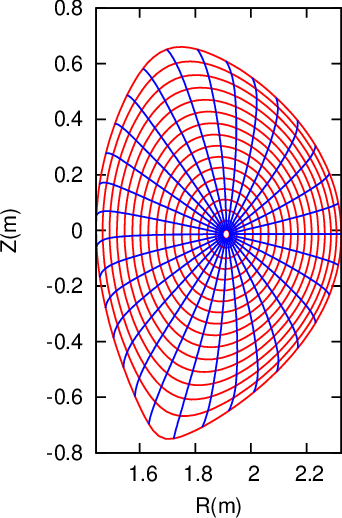
\includegraphics{/home/yj/project_new/read_gfile/fig161/out1.eps}%
\lthtmlpictureZ
\lthtmlcheckvsize\clearpage}

{\newpage\clearpage
\lthtmlpictureA{tex2html_wrap18859}%
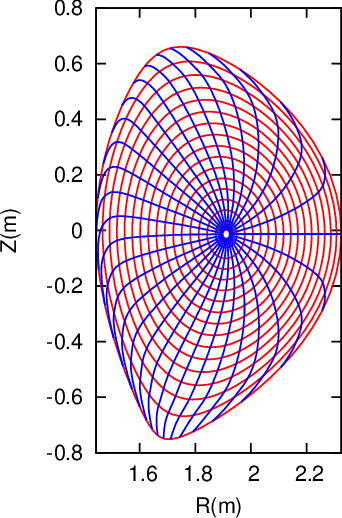
\includegraphics{/home/yj/project_new/read_gfile/fig161/out2.eps}%
\lthtmlpictureZ
\lthtmlcheckvsize\clearpage}

\stepcounter{subsubsection}
{\newpage\clearpage
\lthtmlinlinemathA{tex2html_wrap_indisplay18864}%
$\displaystyle \mathcal{J}_{\ensuremath{\operatorname{new}}} = \frac{1}{(\nabla \psi \times \nabla
   \overline{\theta}) \cdot \nabla \phi}, $%
\lthtmlindisplaymathZ
\lthtmlcheckvsize\clearpage}

{\newpage\clearpage
\lthtmlinlinemathA{tex2html_wrap_indisplay18866}%
$\displaystyle \mathcal{J}_{\ensuremath{\operatorname{new}}} = R (R_{\overline{\theta}} Z_{\psi} - R_{\psi}   Z_{\overline{\theta}}),$%
\lthtmlindisplaymathZ
\lthtmlcheckvsize\clearpage}

\stepcounter{subsubsection}
{\newpage\clearpage
\lthtmlinlinemathA{tex2html_wrap_inline18893}%
$ \mathcal{J}^{- 1} = \nabla \psi \times \nabla \theta \cdot \nabla \phi$%
\lthtmlinlinemathZ
\lthtmlcheckvsize\clearpage}

{\newpage\clearpage
\lthtmlinlinemathA{tex2html_wrap_inline18907}%
$ \sqrt{\overline{\Psi}}$%
\lthtmlinlinemathZ
\lthtmlcheckvsize\clearpage}

{\newpage\clearpage
\lthtmlinlinemathA{tex2html_wrap_indisplay18911}%
$\displaystyle \overline{\Psi} = \frac{\Psi - \Psi_0}{\Psi_a - \Psi_0},$%
\lthtmlindisplaymathZ
\lthtmlcheckvsize\clearpage}

{\newpage\clearpage
\lthtmlinlinemathA{tex2html_wrap_inline18915}%
$ \Psi_a$%
\lthtmlinlinemathZ
\lthtmlcheckvsize\clearpage}

{\newpage\clearpage
\lthtmlinlinemathA{tex2html_wrap_inline18921}%
$ \overline{\Psi}_t$%
\lthtmlinlinemathZ
\lthtmlcheckvsize\clearpage}

{\newpage\clearpage
\lthtmlinlinemathA{tex2html_wrap_inline18925}%
$ \Psi_t$%
\lthtmlinlinemathZ
\lthtmlcheckvsize\clearpage}

{\newpage\clearpage
\lthtmlinlinemathA{tex2html_wrap_indisplay18929}%
$\displaystyle \frac{d \Psi_t}{d \Psi} = 2 \pi q, \Psi_t (0) = 0$%
\lthtmlindisplaymathZ
\lthtmlcheckvsize\clearpage}

{\newpage\clearpage
\lthtmlinlinemathA{tex2html_wrap_indisplay18931}%
$\displaystyle \overline{\Psi}_t = \frac{\Psi_t}{\Psi_t (1)},$%
\lthtmlindisplaymathZ
\lthtmlcheckvsize\clearpage}

{\newpage\clearpage
\lthtmlinlinemathA{tex2html_wrap_inline18933}%
$ \Psi_t (0)$%
\lthtmlinlinemathZ
\lthtmlcheckvsize\clearpage}

{\newpage\clearpage
\lthtmlinlinemathA{tex2html_wrap_inline18935}%
$ \Psi_t (1)$%
\lthtmlinlinemathZ
\lthtmlcheckvsize\clearpage}

{\newpage\clearpage
\lthtmlinlinemathA{tex2html_wrap_inline18939}%
$ \psi = \sqrt{\overline{\Psi}_t}$%
\lthtmlinlinemathZ
\lthtmlcheckvsize\clearpage}

{\newpage\clearpage
\lthtmlinlinemathA{tex2html_wrap_indisplay18941}%
$\displaystyle \frac{d \Psi}{d \psi} = \frac{d \Psi}{d \Psi_t}  \frac{d \Psi_t}{d \psi} =   \frac{1}{2 \pi q}  \frac{d \Psi_t}{d \psi} = \frac{1}{2 \pi q}  \frac{d   \Psi_t}{d \overline{\Psi_t}}  \frac{d \overline{\Psi}_t}{d \psi} =   \frac{1}{2 \pi q} \Psi_t (1) 2 \psi$%
\lthtmlindisplaymathZ
\lthtmlcheckvsize\clearpage}

\stepcounter{section}
{\newpage\clearpage
\lthtmlinlinemathA{tex2html_wrap_inline18956}%
$ \phi = \ensuremath{\operatorname{const}}$%
\lthtmlinlinemathZ
\lthtmlcheckvsize\clearpage}

\stepcounter{subsection}
{\newpage\clearpage
\lthtmlinlinemathA{tex2html_wrap_inline18987}%
$ Z = Z (R)$%
\lthtmlinlinemathZ
\lthtmlcheckvsize\clearpage}

{\newpage\clearpage
\lthtmlinlinemathA{tex2html_wrap_inline18991}%
$ h = \Psi (R, Z
(R))$%
\lthtmlinlinemathZ
\lthtmlcheckvsize\clearpage}

{\newpage\clearpage
\lthtmlinlinemathA{tex2html_wrap_inline18995}%
$ \Psi_i$%
\lthtmlinlinemathZ
\lthtmlcheckvsize\clearpage}

{\newpage\clearpage
\lthtmlinlinemathA{tex2html_wrap_inline18997}%
$ \Psi (R, Z (R)) -
\Psi_i = 0$%
\lthtmlinlinemathZ
\lthtmlcheckvsize\clearpage}

{\newpage\clearpage
\lthtmlpictureA{tex2html_wrap19009}%
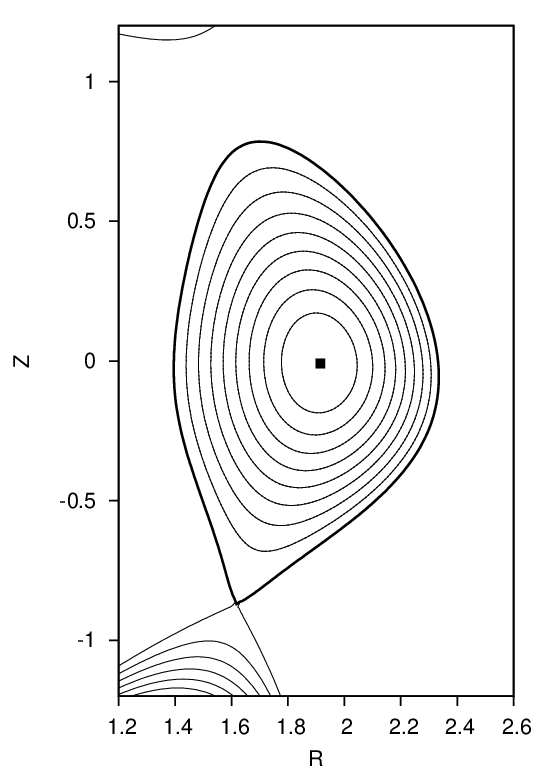
\includegraphics{/home/yj/project_new/read_gfile/fig1/contour.eps}%
\lthtmlpictureZ
\lthtmlcheckvsize\clearpage}

{\newpage\clearpage
\lthtmlinlinemathA{tex2html_wrap_inline19015}%
$ R = R (Z)$%
\lthtmlinlinemathZ
\lthtmlcheckvsize\clearpage}

{\newpage\clearpage
\lthtmlinlinemathA{tex2html_wrap_inline19021}%
$ |d Z / d R| > 1$%
\lthtmlinlinemathZ
\lthtmlcheckvsize\clearpage}

{\newpage\clearpage
\lthtmlinlinemathA{tex2html_wrap_indisplay19031}%
$\displaystyle | \nabla \Psi | = \sqrt{\left( \frac{\partial \Psi}{\partial R} \right)^2 +   \left( \frac{\partial \Psi}{\partial Z} \right)^2},$%
\lthtmlindisplaymathZ
\lthtmlcheckvsize\clearpage}

{\newpage\clearpage
\lthtmlpictureA{tex2html_wrap19045}%
\includegraphics{/home/yj/project_new/read_gfile/fig2/plt.eps}%
\lthtmlpictureZ
\lthtmlcheckvsize\clearpage}

{\newpage\clearpage
\lthtmlpictureA{tex2html_wrap19046}%
\includegraphics{/home/yj/project_new/read_gfile/fig40/plt.eps}%
\lthtmlpictureZ
\lthtmlcheckvsize\clearpage}

{\newpage\clearpage
\lthtmlpictureA{tex2html_wrap19058}%
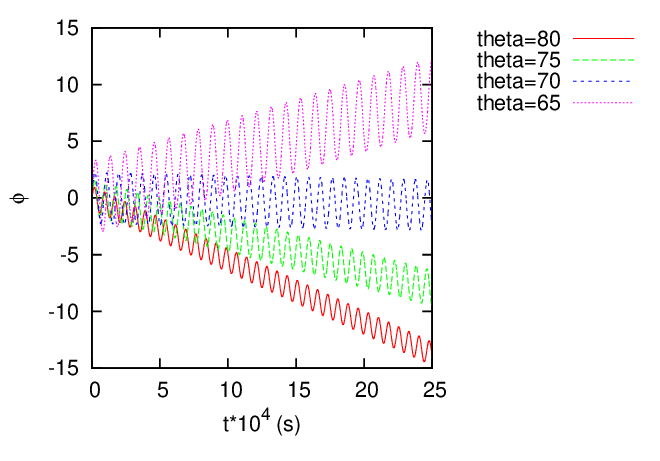
\includegraphics{/home/yj/project_new/read_gfile/fig41/p2.eps}%
\lthtmlpictureZ
\lthtmlcheckvsize\clearpage}

{\newpage\clearpage
\lthtmlpictureA{tex2html_wrap19070}%
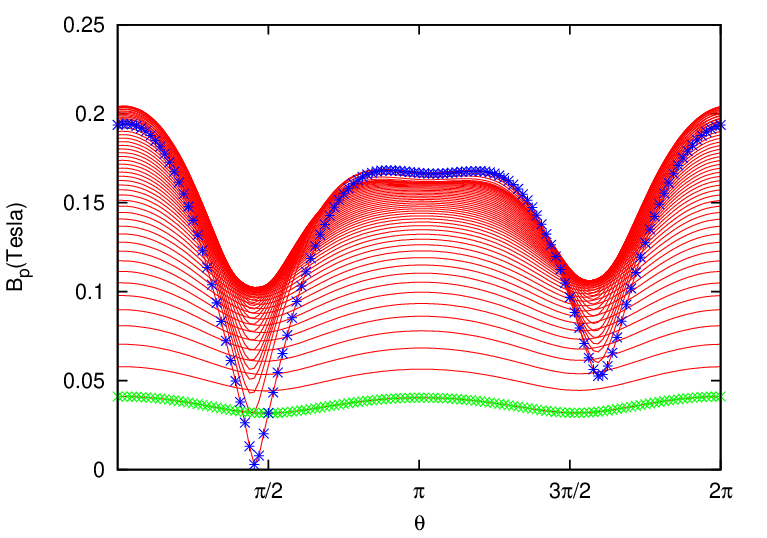
\includegraphics{/home/yj/project_new/read_gfile/fig41/p3.eps}%
\lthtmlpictureZ
\lthtmlcheckvsize\clearpage}

{\newpage\clearpage
\lthtmlpictureA{tex2html_wrap19071}%
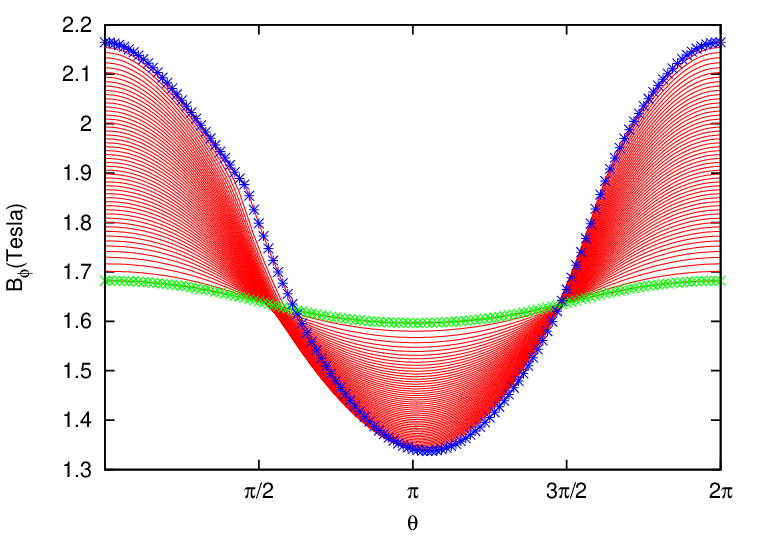
\includegraphics{/home/yj/project_new/read_gfile/fig41/p4.eps}%
\lthtmlpictureZ
\lthtmlcheckvsize\clearpage}

{\newpage\clearpage
\lthtmlpictureA{tex2html_wrap19075}%
\includegraphics{/home/yj/project_new/read_gfile/fig41/tmp.eps}%
\lthtmlpictureZ
\lthtmlcheckvsize\clearpage}

{\newpage\clearpage
\lthtmlpictureA{tex2html_wrap19091}%
\includegraphics{/home/yj/project_new/read_gfile/fig32/tmp.eps}%
\lthtmlpictureZ
\lthtmlcheckvsize\clearpage}

{\newpage\clearpage
\lthtmlpictureA{tex2html_wrap19095}%
\includegraphics{/home/yj/project_new/read_gfile/fig29/tmp.eps}%
\lthtmlpictureZ
\lthtmlcheckvsize\clearpage}

\stepcounter{subsection}
{\newpage\clearpage
\lthtmlinlinemathA{tex2html_wrap_inline19098}%
$ G$%
\lthtmlinlinemathZ
\lthtmlcheckvsize\clearpage}

{\newpage\clearpage
\lthtmlinlinemathA{tex2html_wrap_indisplay19100}%
$\displaystyle \langle G \rangle \equiv \lim_{\Delta \Psi \rightarrow 0}   \left( \frac{\int \int \int_{\Delta \Psi} G d^3 V}{\int \int \int_{\Delta   \Psi} d^3 V} \right),$%
\lthtmlindisplaymathZ
\lthtmlcheckvsize\clearpage}

{\newpage\clearpage
\lthtmlinlinemathA{tex2html_wrap_inline19104}%
$ \triangle \Psi$%
\lthtmlinlinemathZ
\lthtmlcheckvsize\clearpage}

{\newpage\clearpage
\lthtmlinlinemathA{tex2html_wrap_inline19106}%
$ d^3 V = | \mathcal{J} | d \psi d \theta d \phi$%
\lthtmlinlinemathZ
\lthtmlcheckvsize\clearpage}

{\newpage\clearpage
\lthtmlinlinemathA{tex2html_wrap_indisplay19113}%
$\displaystyle \langle G \rangle$%
\lthtmlindisplaymathZ
\lthtmlcheckvsize\clearpage}

{\newpage\clearpage
\lthtmlinlinemathA{tex2html_wrap_indisplay19117}%
$\displaystyle \lim_{\Delta \Psi \rightarrow 0} \left( \frac{\int
\int \int_{\Delta \Psi} G | \mathcal{J} | d \psi d \theta d \phi}{\int \int
\int_{\Delta \Psi} | \mathcal{J} | d \psi d \theta d \phi} \right)$%
\lthtmlindisplaymathZ
\lthtmlcheckvsize\clearpage}

{\newpage\clearpage
\lthtmlinlinemathA{tex2html_wrap_indisplay19121}%
$\displaystyle \frac{\int \int G | \mathcal{J} | d \theta d \phi}{\int \int |
\mathcal{J} | d \theta d \phi},$%
\lthtmlindisplaymathZ
\lthtmlcheckvsize\clearpage}

{\newpage\clearpage
\lthtmlinlinemathA{tex2html_wrap_indisplay19123}%
$\displaystyle d^3 V = R d \phi \frac{d \Psi}{| \nabla \Psi |} d l_p .$%
\lthtmlindisplaymathZ
\lthtmlcheckvsize\clearpage}

{\newpage\clearpage
\lthtmlinlinemathA{tex2html_wrap_indisplay19127}%
$\displaystyle d^3 V = d \phi \frac{d \Psi}{B_p} d l_p$%
\lthtmlindisplaymathZ
\lthtmlcheckvsize\clearpage}

{\newpage\clearpage
\lthtmlinlinemathA{tex2html_wrap_indisplay19134}%
$\displaystyle \lim_{\Delta \Psi \rightarrow 0} \frac{\int \int
\int_{\Delta \Psi} G d \phi \frac{d \Psi}{B_p} d l_p}{\int \int \int_{\Delta
\Psi} d \phi \frac{d \Psi}{B_p} d l_p}$%
\lthtmlindisplaymathZ
\lthtmlcheckvsize\clearpage}

{\newpage\clearpage
\lthtmlinlinemathA{tex2html_wrap_indisplay19138}%
$\displaystyle \frac{\int \int G \frac{1}{B_p} d \phi d l_p}{\int \int \frac{1}{B_p}
d \phi d l_p} .$%
\lthtmlindisplaymathZ
\lthtmlcheckvsize\clearpage}

{\newpage\clearpage
\lthtmlinlinemathA{tex2html_wrap_indisplay19142}%
$\displaystyle \langle G \rangle = \frac{\oint G \frac{1}{B_p} d l_p}{\oint   \frac{1}{B_p} d l_p} .$%
\lthtmlindisplaymathZ
\lthtmlcheckvsize\clearpage}

{\newpage\clearpage
\lthtmlinlinemathA{tex2html_wrap_indisplay19146}%
$\displaystyle \langle G \rangle = \frac{\int_0^{2 \pi} G |\mathcal{J}| d   \theta}{\int_0^{2 \pi} |\mathcal{J}| d \theta} .$%
\lthtmlindisplaymathZ
\lthtmlcheckvsize\clearpage}

{\newpage\clearpage
\lthtmlinlinemathA{tex2html_wrap_indisplay19148}%
$\displaystyle \langle G \rangle = \frac{\int_0^{2 \pi} G\mathcal{J}d \theta}{\int_0^{2   \pi} \mathcal{J}d \theta} .$%
\lthtmlindisplaymathZ
\lthtmlcheckvsize\clearpage}

{\newpage\clearpage
\lthtmlinlinemathA{tex2html_wrap_inline19150}%
$ d \tau = |\mathcal{J}| d \theta d
\phi d \psi$%
\lthtmlinlinemathZ
\lthtmlcheckvsize\clearpage}

{\newpage\clearpage
\lthtmlinlinemathA{tex2html_wrap_indisplay19152}%
$\displaystyle V (\psi) = \int d \tau = \int |\mathcal{J}| d \theta d \phi d   \psi = 2 \pi \int_{\psi_0}^{\psi} \int_0^{2 \pi} |\mathcal{J}| d \theta d   \psi .$%
\lthtmlindisplaymathZ
\lthtmlcheckvsize\clearpage}

{\newpage\clearpage
\lthtmlinlinemathA{tex2html_wrap_inline19154}%
$ V$%
\lthtmlinlinemathZ
\lthtmlcheckvsize\clearpage}

{\newpage\clearpage
\lthtmlinlinemathA{tex2html_wrap_indisplay19158}%
$\displaystyle V' \equiv \frac{d V}{d \psi} = 2 \pi \int_0^{2 \pi}   |\mathcal{J}| d \theta .$%
\lthtmlindisplaymathZ
\lthtmlcheckvsize\clearpage}

{\newpage\clearpage
\lthtmlinlinemathA{tex2html_wrap_indisplay19160}%
$\displaystyle \langle G \rangle = \frac{2 \pi}{V'} \int_0^{2 \pi} G |\mathcal{J}| d \theta$%
\lthtmlindisplaymathZ
\lthtmlcheckvsize\clearpage}

\stepcounter{subsection}
{\newpage\clearpage
\lthtmlinlinemathA{tex2html_wrap_indisplay19163}%
$\displaystyle D (\psi) \equiv \int_V \mathbf{B} \cdot \nabla \theta d \tau,$%
\lthtmlindisplaymathZ
\lthtmlcheckvsize\clearpage}

{\newpage\clearpage
\lthtmlinlinemathA{tex2html_wrap_inline19165}%
$ V = V (\psi)$%
\lthtmlinlinemathZ
\lthtmlcheckvsize\clearpage}

{\newpage\clearpage
\lthtmlinlinemathA{tex2html_wrap_inline19171}%
$ D$%
\lthtmlinlinemathZ
\lthtmlcheckvsize\clearpage}

{\newpage\clearpage
\lthtmlinlinemathA{tex2html_wrap_indisplay19173}%
$\displaystyle D = \int_V \nabla \cdot (\theta \mathbf{B}) d \tau .$%
\lthtmlindisplaymathZ
\lthtmlcheckvsize\clearpage}

{\newpage\clearpage
\lthtmlinlinemathA{tex2html_wrap_inline19179}%
$ 0 \leqslant \theta < 2
\pi$%
\lthtmlinlinemathZ
\lthtmlcheckvsize\clearpage}

{\newpage\clearpage
\lthtmlinlinemathA{tex2html_wrap_inline19181}%
$ \theta = \theta (R, Z)$%
\lthtmlinlinemathZ
\lthtmlcheckvsize\clearpage}

{\newpage\clearpage
\lthtmlinlinemathA{tex2html_wrap_inline19185}%
$ \theta \mathbf{B}$%
\lthtmlinlinemathZ
\lthtmlcheckvsize\clearpage}

{\newpage\clearpage
\lthtmlinlinemathA{tex2html_wrap_indisplay19194}%
$\displaystyle D$%
\lthtmlindisplaymathZ
\lthtmlcheckvsize\clearpage}

{\newpage\clearpage
\lthtmlinlinemathA{tex2html_wrap_indisplay19198}%
$\displaystyle \int_{S_1} \theta \mathbf{B} \cdot d\mathbf{S}+ \int_{S_2} \theta
\mathbf{B} \cdot d\mathbf{S}+ \int_{S_3} \theta \mathbf{B} \cdot
d\mathbf{S},$%
\lthtmlindisplaymathZ
\lthtmlcheckvsize\clearpage}

{\newpage\clearpage
\lthtmlinlinemathA{tex2html_wrap_inline19210}%
$ \psi = \psi_0$%
\lthtmlinlinemathZ
\lthtmlcheckvsize\clearpage}

{\newpage\clearpage
\lthtmlinlinemathA{tex2html_wrap_indisplay19221}%
$\displaystyle \int_{S_1} \theta \mathbf{B} \cdot d\mathbf{S}+ \int_{S_2} \theta
\mathbf{B} \cdot d\mathbf{S}+ 0$%
\lthtmlindisplaymathZ
\lthtmlcheckvsize\clearpage}

{\newpage\clearpage
\lthtmlinlinemathA{tex2html_wrap_indisplay19225}%
$\displaystyle \int_{S_1} 0\mathbf{B} \cdot d\mathbf{S}+ \int_{S_2} 2 \pi \mathbf{B}
\cdot d\mathbf{S}$%
\lthtmlindisplaymathZ
\lthtmlcheckvsize\clearpage}

{\newpage\clearpage
\lthtmlinlinemathA{tex2html_wrap_indisplay19229}%
$\displaystyle 2 \pi \int_{S_2} \mathbf{B} \cdot d\mathbf{S}.$%
\lthtmlindisplaymathZ
\lthtmlcheckvsize\clearpage}

{\newpage\clearpage
\lthtmlinlinemathA{tex2html_wrap_indisplay19239}%
$\displaystyle \Psi_p = \frac{1}{2 \pi} D = \frac{1}{2 \pi} \int_V \mathbf{B} \cdot \nabla   \theta d \tau .$%
\lthtmlindisplaymathZ
\lthtmlcheckvsize\clearpage}

{\newpage\clearpage
\lthtmlinlinemathA{tex2html_wrap_indisplay19250}%
$\displaystyle \frac{1}{2 \pi} \int_V \mathbf{B} \cdot \nabla \theta
|\mathcal{J}| d \theta d \phi d \psi$%
\lthtmlindisplaymathZ
\lthtmlcheckvsize\clearpage}

{\newpage\clearpage
\lthtmlinlinemathA{tex2html_wrap_indisplay19254}%
$\displaystyle \int_0^{\psi} d \psi \int_0^{2 \pi} \mathbf{B} \cdot \nabla \theta
|\mathcal{J}| d \theta$%
\lthtmlindisplaymathZ
\lthtmlcheckvsize\clearpage}

{\newpage\clearpage
\lthtmlinlinemathA{tex2html_wrap_indisplay19258}%
$\displaystyle \int_0^{\psi} d \psi \int_0^{2 \pi} \Psi' \nabla \psi \times \nabla
\phi \cdot \nabla \theta |\mathcal{J}| d \theta$%
\lthtmlindisplaymathZ
\lthtmlcheckvsize\clearpage}

{\newpage\clearpage
\lthtmlinlinemathA{tex2html_wrap_indisplay19262}%
$\displaystyle - \ensuremath{\operatorname{sign}} (\mathcal{J}) \int_0^{\psi} d \psi \int_0^{2 \pi} \Psi'
(\psi) d \theta$%
\lthtmlindisplaymathZ
\lthtmlcheckvsize\clearpage}

{\newpage\clearpage
\lthtmlinlinemathA{tex2html_wrap_indisplay19266}%
$\displaystyle - 2 \pi \ensuremath{\operatorname{sign}} (\mathcal{J}) \int_0^{\psi} \Psi' (\psi) d \psi$%
\lthtmlindisplaymathZ
\lthtmlcheckvsize\clearpage}

{\newpage\clearpage
\lthtmlinlinemathA{tex2html_wrap_indisplay19270}%
$\displaystyle - 2 \pi \ensuremath{\operatorname{sign}} (\mathcal{J}) [\Psi (\psi) - \Psi (0)] .$%
\lthtmlindisplaymathZ
\lthtmlcheckvsize\clearpage}

{\newpage\clearpage
\lthtmlinlinemathA{tex2html_wrap_indisplay19280}%
$\displaystyle \Psi_t = \frac{1}{2 \pi} \int_V \mathbf{B} \cdot \nabla \phi d \tau,$%
\lthtmlindisplaymathZ
\lthtmlcheckvsize\clearpage}

{\newpage\clearpage
\lthtmlinlinemathA{tex2html_wrap_indisplay19282}%
$\displaystyle K (\psi) = \frac{1}{2 \pi} \int_V \mathbf{J} \cdot \nabla \theta d \tau,$%
\lthtmlindisplaymathZ
\lthtmlcheckvsize\clearpage}

{\newpage\clearpage
\lthtmlinlinemathA{tex2html_wrap_indisplay19284}%
$\displaystyle I (\psi) = \frac{1}{2 \pi} \int_V \mathbf{J} \cdot \nabla   \phi d \tau .$%
\lthtmlindisplaymathZ
\lthtmlcheckvsize\clearpage}

{\newpage\clearpage
\lthtmlinlinemathA{tex2html_wrap_indisplay19287}%
$\displaystyle \Psi_t$%
\lthtmlindisplaymathZ
\lthtmlcheckvsize\clearpage}

{\newpage\clearpage
\lthtmlinlinemathA{tex2html_wrap_indisplay19291}%
$\displaystyle \frac{1}{2 \pi} \int \mathbf{B} \cdot \nabla \phi |\mathcal{J}|
d \theta d \phi d \psi$%
\lthtmlindisplaymathZ
\lthtmlcheckvsize\clearpage}

{\newpage\clearpage
\lthtmlinlinemathA{tex2html_wrap_indisplay19295}%
$\displaystyle \int_0^{\psi} d \psi \int_0^{2 \pi} g \frac{1}{R^2} |\mathcal{J}| d
\theta$%
\lthtmlindisplaymathZ
\lthtmlcheckvsize\clearpage}

{\newpage\clearpage
\lthtmlinlinemathA{tex2html_wrap_indisplay19299}%
$\displaystyle \int_0^{\psi} \left[ g \frac{V'}{2 \pi} \left\langle \frac{1}{R^2}
\right\rangle \right] d \psi .$%
\lthtmlindisplaymathZ
\lthtmlcheckvsize\clearpage}

{\newpage\clearpage
\lthtmlinlinemathA{tex2html_wrap_indisplay19301}%
$\displaystyle \Rightarrow \Psi_t' = g \frac{V'}{2 \pi} \left\langle \frac{1}{R^2}
   \right\rangle $%
\lthtmlindisplaymathZ
\lthtmlcheckvsize\clearpage}

{\newpage\clearpage
\lthtmlinlinemathA{tex2html_wrap_indisplay19303}%
$\displaystyle \Rightarrow \frac{d \Psi_t}{d V} = g \frac{1}{2 \pi} \left\langle
   \frac{1}{R^2} \right\rangle $%
\lthtmlindisplaymathZ
\lthtmlcheckvsize\clearpage}

{\newpage\clearpage
\lthtmlinlinemathA{tex2html_wrap_indisplay19305}%
$\displaystyle \Rightarrow \frac{d \Psi}{d V} = \frac{g}{2 \pi q}  \frac{1}{2 \pi}   \left\langle \frac{1}{R^2} \right\rangle .$%
\lthtmlindisplaymathZ
\lthtmlcheckvsize\clearpage}

{\newpage\clearpage
\lthtmlinlinemathA{tex2html_wrap_indisplay19308}%
$\displaystyle \frac{d \Psi_t}{d \Psi_p}$%
\lthtmlindisplaymathZ
\lthtmlcheckvsize\clearpage}

{\newpage\clearpage
\lthtmlinlinemathA{tex2html_wrap_indisplay19312}%
$\displaystyle \frac{\Psi_t'}{\Psi_p'}$%
\lthtmlindisplaymathZ
\lthtmlcheckvsize\clearpage}

{\newpage\clearpage
\lthtmlinlinemathA{tex2html_wrap_indisplay19316}%
$\displaystyle - \frac{g V'}{(2 \pi)^2 \Psi'}  \left\langle \frac{1}{R^2}
\right\rangle,$%
\lthtmlindisplaymathZ
\lthtmlcheckvsize\clearpage}

{\newpage\clearpage
\lthtmlinlinemathA{tex2html_wrap_indisplay19318}%
$\displaystyle \frac{d \Psi_t}{d \Psi_p} = q (\psi) .$%
\lthtmlindisplaymathZ
\lthtmlcheckvsize\clearpage}

{\newpage\clearpage
\lthtmlinlinemathA{tex2html_wrap_indisplay19320}%
$\displaystyle - \ensuremath{\operatorname{sgn}} (\mathcal{J}) \frac{V'}{(2 \pi)^2}  \frac{g}{\Psi'} \langle
   R^{- 2} \rangle $%
\lthtmlindisplaymathZ
\lthtmlcheckvsize\clearpage}

{\newpage\clearpage
\lthtmlinlinemathA{tex2html_wrap_indisplay19323}%
$\displaystyle K (\psi)$%
\lthtmlindisplaymathZ
\lthtmlcheckvsize\clearpage}

{\newpage\clearpage
\lthtmlinlinemathA{tex2html_wrap_indisplay19327}%
$\displaystyle \frac{1}{2 \pi} \int \mathbf{J} \cdot \nabla \theta
\mathcal{J}d \theta d \phi d \psi$%
\lthtmlindisplaymathZ
\lthtmlcheckvsize\clearpage}

{\newpage\clearpage
\lthtmlinlinemathA{tex2html_wrap_indisplay19331}%
$\displaystyle \frac{1}{\mu_0} \int (- g') \nabla \phi \times \nabla \psi \cdot
\nabla \theta \mathcal{J}d \theta d \psi$%
\lthtmlindisplaymathZ
\lthtmlcheckvsize\clearpage}

{\newpage\clearpage
\lthtmlinlinemathA{tex2html_wrap_indisplay19335}%
$\displaystyle - \frac{1}{\mu_0} \int g' d \theta d \psi$%
\lthtmlindisplaymathZ
\lthtmlcheckvsize\clearpage}

{\newpage\clearpage
\lthtmlinlinemathA{tex2html_wrap_indisplay19339}%
$\displaystyle - \frac{2 \pi}{\mu_0} \int_0^{\psi} g' d \psi$%
\lthtmlindisplaymathZ
\lthtmlcheckvsize\clearpage}

{\newpage\clearpage
\lthtmlinlinemathA{tex2html_wrap_indisplay19343}%
$\displaystyle - \frac{2 \pi}{\mu_0} [g (\psi) - g (0)] .$%
\lthtmlindisplaymathZ
\lthtmlcheckvsize\clearpage}

{\newpage\clearpage
\lthtmlinlinemathA{tex2html_wrap_indisplay19349}%
$\displaystyle - \left[ \left( \Psi' \frac{\mathcal{J}}{R^2} | \nabla \psi |^2
   \right)_{\psi} + \left( \Psi' \frac{\mathcal{J}}{R^2} \nabla \psi \cdot
   \nabla \theta \right)_{\theta} \right] \nabla \psi \times \nabla \theta -
   g' \nabla \phi \times \nabla \psi, $%
\lthtmlindisplaymathZ
\lthtmlcheckvsize\clearpage}

{\newpage\clearpage
\lthtmlinlinemathA{tex2html_wrap_indisplay19352}%
$\displaystyle I_{\phi} (\psi)$%
\lthtmlindisplaymathZ
\lthtmlcheckvsize\clearpage}

{\newpage\clearpage
\lthtmlinlinemathA{tex2html_wrap_indisplay19356}%
$\displaystyle \frac{1}{2 \pi} \int \mathbf{J} \cdot \nabla \phi
\mathcal{J}d \theta d \phi d \psi$%
\lthtmlindisplaymathZ
\lthtmlcheckvsize\clearpage}

{\newpage\clearpage
\lthtmlinlinemathA{tex2html_wrap_indisplay19360}%
$\displaystyle - \frac{1}{2 \pi \mu_0} \int \left[ \left( \Psi'
\frac{\mathcal{J}}{R^2} | \nabla \psi |^2 \right)_{\psi} + \left( \Psi'
\frac{\mathcal{J}}{R^2} \nabla \psi \cdot \nabla \theta \right)_{\theta}
\right] \nabla \psi \times \nabla \theta \cdot \nabla \phi \mathcal{J}d
\theta d \phi d \psi$%
\lthtmlindisplaymathZ
\lthtmlcheckvsize\clearpage}

{\newpage\clearpage
\lthtmlinlinemathA{tex2html_wrap_indisplay19364}%
$\displaystyle - \frac{1}{\mu_0} \int \left[ \left( \Psi' \frac{\mathcal{J}}{R^2} |
\nabla \psi |^2 \right)_{\psi} + \left( \Psi' \frac{\mathcal{J}}{R^2} \nabla
\psi \cdot \nabla \theta \right)_{\theta} \right] d \theta d \psi$%
\lthtmlindisplaymathZ
\lthtmlcheckvsize\clearpage}

{\newpage\clearpage
\lthtmlinlinemathA{tex2html_wrap_indisplay19368}%
$\displaystyle - \frac{1}{\mu_0} \int \left[ \left( \Psi' \frac{\mathcal{J}}{R^2} |
\nabla \psi |^2 \right)_{\psi} \right] d \theta d \psi$%
\lthtmlindisplaymathZ
\lthtmlcheckvsize\clearpage}

{\newpage\clearpage
\lthtmlinlinemathA{tex2html_wrap_indisplay19372}%
$\displaystyle - \frac{1}{\mu_0} \int_0^{2 \pi} d \theta \int_0^{\psi} d \psi \left(
\Psi' \frac{\mathcal{J}}{R^2} | \nabla \psi |^2 \right)_{\psi}$%
\lthtmlindisplaymathZ
\lthtmlcheckvsize\clearpage}

{\newpage\clearpage
\lthtmlinlinemathA{tex2html_wrap_indisplay19376}%
$\displaystyle - \frac{1}{\mu_0} \int_0^{2 \pi} d \theta \left( \Psi'
\frac{\mathcal{J}}{R^2} | \nabla \psi |^2 - 0 \right) .$%
\lthtmlindisplaymathZ
\lthtmlcheckvsize\clearpage}

{\newpage\clearpage
\lthtmlinlinemathA{tex2html_wrap_inline19378}%
$ \nabla \psi = 0$%
\lthtmlinlinemathZ
\lthtmlcheckvsize\clearpage}

{\newpage\clearpage
\lthtmlinlinemathA{tex2html_wrap_inline19380}%
$ \psi = 0$%
\lthtmlinlinemathZ
\lthtmlcheckvsize\clearpage}

{\newpage\clearpage
\lthtmlinlinemathA{tex2html_wrap_indisplay19382}%
$\displaystyle I_{\phi} (\psi) = - \frac{V' \Psi'}{2 \pi \mu_0} \left\langle \frac{| \nabla   \psi |^2}{R^2} \right\rangle .$%
\lthtmlindisplaymathZ
\lthtmlcheckvsize\clearpage}

{\newpage\clearpage
\lthtmlinlinemathA{tex2html_wrap_indisplay19385}%
$\displaystyle \frac{\langle \mathbf{J} \cdot \mathbf{B} \rangle}{\langle \mathbf{B} \cdot
\nabla \phi \rangle}$%
\lthtmlindisplaymathZ
\lthtmlcheckvsize\clearpage}

{\newpage\clearpage
\lthtmlinlinemathA{tex2html_wrap_indisplay19389}%
$\displaystyle \frac{\left\langle \frac{g^2}{\mathcal{J}} \left[
\left( \frac{1}{g} \Psi' \frac{\mathcal{J}}{R^2} | \nabla \psi |^2
\right)_{\psi} + \left( \frac{1}{g} \Psi' \nabla \psi \cdot \nabla \theta
\frac{\mathcal{J}}{R^2} \right)_{\theta} \right] \right\rangle}{\mu_0
\langle g / R^2 \rangle}$%
\lthtmlindisplaymathZ
\lthtmlcheckvsize\clearpage}

{\newpage\clearpage
\lthtmlinlinemathA{tex2html_wrap_indisplay19393}%
$\displaystyle \frac{\frac{2 \pi}{V'} \int_0^{2 \pi} d \theta g^2 \left[ \left(
\frac{1}{g} \Psi' \frac{\mathcal{J}}{R^2} | \nabla \psi |^2 \right)_{\psi} +
\left( \frac{1}{g} \Psi' \nabla \psi \cdot \nabla \theta
\frac{\mathcal{J}}{R^2} \right)_{\theta} \right]}{\mu_0 g \langle R^{- 2}
\rangle}$%
\lthtmlindisplaymathZ
\lthtmlcheckvsize\clearpage}

{\newpage\clearpage
\lthtmlinlinemathA{tex2html_wrap_indisplay19397}%
$\displaystyle \frac{\frac{2 \pi}{V'} g^2 \int_0^{2 \pi} d \theta \left[ \left(
\frac{1}{g} \Psi' \frac{\mathcal{J}}{R^2} | \nabla \psi |^2 \right)_{\psi} +
\left( \frac{1}{g} \Psi' \nabla \psi \cdot \nabla \theta
\frac{\mathcal{J}}{R^2} \right)_{\theta} \right]}{\mu_0 g \langle R^{- 2}
\rangle}$%
\lthtmlindisplaymathZ
\lthtmlcheckvsize\clearpage}

{\newpage\clearpage
\lthtmlinlinemathA{tex2html_wrap_indisplay19401}%
$\displaystyle \frac{\frac{2 \pi}{V'} g \int_0^{2 \pi} d \theta \left[ \left(
\frac{1}{g} \Psi' \frac{\mathcal{J}}{R^2} | \nabla \psi |^2 \right)_{\psi}
\right]}{\mu_0 \langle R^{- 2} \rangle}$%
\lthtmlindisplaymathZ
\lthtmlcheckvsize\clearpage}

{\newpage\clearpage
\lthtmlinlinemathA{tex2html_wrap_indisplay19416}%
$\displaystyle \frac{\frac{2 \pi}{V'} g \left[ \frac{1}{g} \Psi'
\left( \int_0^{2 \pi} d \theta \frac{\mathcal{J}}{R^2} | \nabla \psi |^2
\right) \right]_{\psi}}{\mu_0 \langle R^{- 2} \rangle}$%
\lthtmlindisplaymathZ
\lthtmlcheckvsize\clearpage}

{\newpage\clearpage
\lthtmlinlinemathA{tex2html_wrap_indisplay19420}%
$\displaystyle \frac{\frac{1}{V'} g \left[ \frac{1}{g} \Psi' V' \left\langle \frac{|
\nabla \psi |^2}{R^2} \right\rangle \right]_{\psi}}{\mu_0 \langle R^{- 2}
\rangle}$%
\lthtmlindisplaymathZ
\lthtmlcheckvsize\clearpage}

{\newpage\clearpage
\lthtmlinlinemathA{tex2html_wrap_indisplay19424}%
$\displaystyle \frac{g}{\mu_0 V' \langle R^{- 2} \rangle} \left[ \frac{\Psi' V'}{g}
\left\langle \frac{| \nabla \psi |^2}{R^2} \right\rangle \right]_{\psi}$%
\lthtmlindisplaymathZ
\lthtmlcheckvsize\clearpage}

\stepcounter{section}
\stepcounter{subsection}
{\newpage\clearpage
\lthtmlinlinemathA{tex2html_wrap_inline19436}%
$ \mathcal{J}= \alpha (\psi) R^2$%
\lthtmlinlinemathZ
\lthtmlcheckvsize\clearpage}

{\newpage\clearpage
\lthtmlinlinemathA{tex2html_wrap_inline19438}%
$ \alpha (\psi)$%
\lthtmlinlinemathZ
\lthtmlcheckvsize\clearpage}

{\newpage\clearpage
\lthtmlinlinemathA{tex2html_wrap_indisplay19460}%
$\displaystyle \zeta = \phi - q (\psi) \delta (\psi, \theta),$%
\lthtmlindisplaymathZ
\lthtmlcheckvsize\clearpage}

{\newpage\clearpage
\lthtmlinlinemathA{tex2html_wrap_inline19462}%
$ \delta = \delta (\psi, \theta)$%
\lthtmlinlinemathZ
\lthtmlcheckvsize\clearpage}

{\newpage\clearpage
\lthtmlinlinemathA{tex2html_wrap_inline19466}%
$ \mathbf{B} \cdot \nabla \zeta /\mathbf{B} \cdot \nabla \theta$%
\lthtmlinlinemathZ
\lthtmlcheckvsize\clearpage}

{\newpage\clearpage
\lthtmlinlinemathA{tex2html_wrap_indisplay19469}%
$\displaystyle \frac{\mathbf{B} \cdot \nabla \zeta}{\mathbf{B} \cdot \nabla \theta}$%
\lthtmlindisplaymathZ
\lthtmlcheckvsize\clearpage}

{\newpage\clearpage
\lthtmlinlinemathA{tex2html_wrap_indisplay19473}%
$\displaystyle \frac{(\nabla \Psi \times \nabla \phi + g \nabla \phi) \cdot \nabla (\phi -
q \delta)}{(\nabla \Psi \times \nabla \phi + g \nabla \phi) \cdot \nabla
\theta}$%
\lthtmlindisplaymathZ
\lthtmlcheckvsize\clearpage}

{\newpage\clearpage
\lthtmlinlinemathA{tex2html_wrap_indisplay19477}%
$\displaystyle \frac{(\nabla \Psi \times \nabla \phi + g \nabla \phi) \cdot [\nabla
\phi - \nabla (q \delta)]}{(\nabla \Psi \times \nabla \phi) \cdot \nabla
\theta}$%
\lthtmlindisplaymathZ
\lthtmlcheckvsize\clearpage}

{\newpage\clearpage
\lthtmlinlinemathA{tex2html_wrap_indisplay19481}%
$\displaystyle \frac{g | \nabla \phi |^2 + (\nabla \Psi \times \nabla \phi) \cdot [-
\nabla (q \delta)]}{(\nabla \Psi \times \nabla \phi) \cdot \nabla \theta} .$%
\lthtmlindisplaymathZ
\lthtmlcheckvsize\clearpage}

{\newpage\clearpage
\lthtmlinlinemathA{tex2html_wrap_indisplay19490}%
$\displaystyle \frac{g | \nabla \phi |^2 - \Psi' (\nabla \psi \times \nabla \phi) \cdot
\left[ \frac{\partial (q \delta)}{\partial \theta} \nabla \theta +
\frac{\partial (q \delta)}{\partial \psi} \nabla \psi \right]}{- \Psi'
\mathcal{J}^{- 1}}$%
\lthtmlindisplaymathZ
\lthtmlcheckvsize\clearpage}

{\newpage\clearpage
\lthtmlinlinemathA{tex2html_wrap_indisplay19494}%
$\displaystyle - \frac{g}{\Psi'}  \frac{\mathcal{J}}{R^2} - q \frac{\partial
\delta}{\partial \theta},$%
\lthtmlindisplaymathZ
\lthtmlcheckvsize\clearpage}

{\newpage\clearpage
\lthtmlinlinemathA{tex2html_wrap_indisplay19500}%
$\displaystyle \frac{\mathbf{B} \cdot \nabla \zeta}{\mathbf{B} \cdot \nabla \theta} =   \hat{q} - q \frac{\partial \delta}{\partial \theta},$%
\lthtmlindisplaymathZ
\lthtmlcheckvsize\clearpage}

{\newpage\clearpage
\lthtmlinlinemathA{tex2html_wrap_indisplay19506}%
$\displaystyle \hat{q} - q \frac{\partial \delta}{\partial \theta} = c   (\psi),$%
\lthtmlindisplaymathZ
\lthtmlcheckvsize\clearpage}

{\newpage\clearpage
\lthtmlinlinemathA{tex2html_wrap_inline19508}%
$ c (\psi)$%
\lthtmlinlinemathZ
\lthtmlcheckvsize\clearpage}

{\newpage\clearpage
\lthtmlinlinemathA{tex2html_wrap_inline19514}%
$ c (\psi) = q$%
\lthtmlinlinemathZ
\lthtmlcheckvsize\clearpage}

{\newpage\clearpage
\lthtmlinlinemathA{tex2html_wrap_indisplay19516}%
$\displaystyle \frac{\partial \delta}{\partial \theta} = \frac{\hat{q}}{q}   - 1.$%
\lthtmlindisplaymathZ
\lthtmlcheckvsize\clearpage}

{\newpage\clearpage
\lthtmlinlinemathA{tex2html_wrap_indisplay19520}%
$\displaystyle \delta (\psi, \theta) = \delta (\psi, 0) + \frac{1}{q} \int_0^{\theta}   \hat{q} d \theta - \theta .$%
\lthtmlindisplaymathZ
\lthtmlcheckvsize\clearpage}

{\newpage\clearpage
\lthtmlinlinemathA{tex2html_wrap_inline19526}%
$ \delta (\psi, 0)$%
\lthtmlinlinemathZ
\lthtmlcheckvsize\clearpage}

{\newpage\clearpage
\lthtmlinlinemathA{tex2html_wrap_indisplay19528}%
$\displaystyle \delta = \frac{1}{q} \int_0^{\theta} \hat{q} d \theta -   \theta,$%
\lthtmlindisplaymathZ
\lthtmlcheckvsize\clearpage}

{\newpage\clearpage
\lthtmlinlinemathA{tex2html_wrap_indisplay19530}%
$\displaystyle \delta = \frac{1}{q} \int_0^{\theta} \frac{\mathbf{B} \cdot \nabla   \phi}{\mathbf{B} \cdot \nabla \theta} d \theta - \theta$%
\lthtmlindisplaymathZ
\lthtmlcheckvsize\clearpage}

{\newpage\clearpage
\lthtmlinlinemathA{tex2html_wrap_indisplay19534}%
$\displaystyle \zeta = \phi - \int_0^{\theta} \frac{\mathbf{B} \cdot   \nabla \phi}{\mathbf{B} \cdot \nabla \theta} d \theta + q \theta .$%
\lthtmlindisplaymathZ
\lthtmlcheckvsize\clearpage}

{\newpage\clearpage
\lthtmlinlinemathA{tex2html_wrap_inline19542}%
$ \int_0^{\theta} \frac{\mathbf{B} \cdot
\nabla \phi}{\mathbf{B} \cdot \nabla \theta} d \theta$%
\lthtmlinlinemathZ
\lthtmlcheckvsize\clearpage}

{\newpage\clearpage
\lthtmlinlinemathA{tex2html_wrap_indisplay19546}%
$\displaystyle - \int_0^{\theta} \frac{\mathbf{B} \cdot \nabla \phi}{\mathbf{B} \cdot   \nabla \theta} d \theta = - \int_0^{\theta}  \frac{g}{R^2}    \frac{\mathcal{J}}{\Psi'} d \theta = - \int_0^{\theta}  \frac{g}{R^2}    \frac{1}{\Psi'} \frac{R}{| \nabla \psi |} d l_p = - \int_0^{\theta}    \frac{g}{R}  \frac{1}{| \nabla \Psi |} d l_p = - \int_0^{\theta}    \frac{1}{R}  \frac{B_{\phi}}{B_p} d \ell_p .$%
\lthtmlindisplaymathZ
\lthtmlcheckvsize\clearpage}

{\newpage\clearpage
\lthtmlinlinemathA{tex2html_wrap_indisplay19549}%
$\displaystyle \frac{\partial (\delta q)}{\partial \psi}$%
\lthtmlindisplaymathZ
\lthtmlcheckvsize\clearpage}

{\newpage\clearpage
\lthtmlinlinemathA{tex2html_wrap_indisplay19553}%
$\displaystyle - \frac{d}{d \psi} \left(
\frac{g}{\Psi'} \right) \int_0^{\theta} \frac{\mathcal{J}}{R^2} d \theta -
\frac{g}{\Psi'}  \frac{\partial}{\partial \psi} \int_0^{\theta}
\frac{\mathcal{J}}{R^2} d \theta - \frac{d q}{d \psi} \theta .$%
\lthtmlindisplaymathZ
\lthtmlcheckvsize\clearpage}

{\newpage\clearpage
\lthtmlinlinemathA{tex2html_wrap_inline19555}%
$ \partial (\delta q) / \partial
\psi$%
\lthtmlinlinemathZ
\lthtmlcheckvsize\clearpage}

{\newpage\clearpage
\lthtmlinlinemathA{tex2html_wrap_inline19557}%
$ \partial (g / \Psi') / \partial \psi$%
\lthtmlinlinemathZ
\lthtmlcheckvsize\clearpage}

{\newpage\clearpage
\lthtmlinlinemathA{tex2html_wrap_inline19559}%
$ \delta (\psi, \theta)$%
\lthtmlinlinemathZ
\lthtmlcheckvsize\clearpage}

{\newpage\clearpage
\lthtmlinlinemathA{tex2html_wrap_inline19561}%
$ \mathbf{B} \cdot \nabla \zeta /\mathbf{B} \cdot
\nabla \theta = q$%
\lthtmlinlinemathZ
\lthtmlcheckvsize\clearpage}

{\newpage\clearpage
\lthtmlinlinemathA{tex2html_wrap_inline19563}%
$ \delta (\psi, 0) =
\delta (\psi, 2 \pi) = 0$%
\lthtmlinlinemathZ
\lthtmlcheckvsize\clearpage}

{\newpage\clearpage
\lthtmlinlinemathA{tex2html_wrap_indisplay19565}%
$\displaystyle \delta (\psi, \theta = 0) = 0. $%
\lthtmlindisplaymathZ
\lthtmlcheckvsize\clearpage}

{\newpage\clearpage
\lthtmlinlinemathA{tex2html_wrap_indisplay19567}%
$\displaystyle \delta (\psi, \theta = 2 \pi) = \frac{1}{q} \int_0^{2 \pi} \hat{q} d \theta   - 2 \pi = 0,$%
\lthtmlindisplaymathZ
\lthtmlcheckvsize\clearpage}

\stepcounter{subsection}
{\newpage\clearpage
\lthtmlinlinemathA{tex2html_wrap_indisplay19587}%
$\displaystyle - \Psi' \nabla (\zeta + q \delta) \times \nabla \psi -
\Psi' \hat{q} \nabla \psi \times \nabla \theta$%
\lthtmlindisplaymathZ
\lthtmlcheckvsize\clearpage}

{\newpage\clearpage
\lthtmlinlinemathA{tex2html_wrap_indisplay19591}%
$\displaystyle - \Psi' \nabla \zeta \times \nabla \psi - \Psi' \nabla (q \delta)
\times \nabla \psi - \Psi' \hat{q} \nabla \psi \times \nabla \theta$%
\lthtmlindisplaymathZ
\lthtmlcheckvsize\clearpage}

{\newpage\clearpage
\lthtmlinlinemathA{tex2html_wrap_indisplay19595}%
$\displaystyle - \Psi' \nabla \zeta \times \nabla \psi - \Psi' q \frac{\partial
\delta}{\partial \theta} \nabla \theta \times \nabla \psi - \Psi' \hat{q}
\nabla \psi \times \nabla \theta$%
\lthtmlindisplaymathZ
\lthtmlcheckvsize\clearpage}

{\newpage\clearpage
\lthtmlinlinemathA{tex2html_wrap_indisplay19602}%
$\displaystyle - \Psi' (\nabla \zeta \times \nabla \psi + q \nabla \psi
\times \nabla \theta) .$%
\lthtmlindisplaymathZ
\lthtmlcheckvsize\clearpage}

\stepcounter{subsection}
{\newpage\clearpage
\lthtmlinlinemathA{tex2html_wrap_indisplay19611}%
$\displaystyle \frac{d}{d x} = \frac{d}{d (x + c)},$%
\lthtmlindisplaymathZ
\lthtmlcheckvsize\clearpage}

{\newpage\clearpage
\lthtmlinlinemathA{tex2html_wrap_inline19613}%
$ c$%
\lthtmlinlinemathZ
\lthtmlcheckvsize\clearpage}

{\newpage\clearpage
\lthtmlinlinemathA{tex2html_wrap_indisplay19615}%
$\displaystyle \left( \frac{\partial f}{\partial \zeta} \right)_{\psi, \theta} = \left(   \frac{\partial f}{\partial \phi} \right)_{\psi, \theta},$%
\lthtmlindisplaymathZ
\lthtmlcheckvsize\clearpage}

{\newpage\clearpage
\lthtmlinlinemathA{tex2html_wrap_inline19617}%
$ \phi = \zeta + q (\psi) \delta (\psi, \theta)$%
\lthtmlinlinemathZ
\lthtmlcheckvsize\clearpage}

{\newpage\clearpage
\lthtmlinlinemathA{tex2html_wrap_inline19619}%
$ q
(\psi) \delta (\psi, \theta)$%
\lthtmlinlinemathZ
\lthtmlcheckvsize\clearpage}

{\newpage\clearpage
\lthtmlinlinemathA{tex2html_wrap_indisplay19629}%
$\displaystyle \left( \frac{\partial f}{\partial \psi} \right)_{\theta,   \zeta} \neq \left( \frac{\partial f}{\partial \psi} \right)_{\theta, \phi}$%
\lthtmlindisplaymathZ
\lthtmlcheckvsize\clearpage}

{\newpage\clearpage
\lthtmlinlinemathA{tex2html_wrap_indisplay19631}%
$\displaystyle \left( \frac{\partial f}{\partial \theta} \right)_{\psi,   \zeta} \neq \left( \frac{\partial f}{\partial \theta} \right)_{\psi, \phi} .$%
\lthtmlindisplaymathZ
\lthtmlcheckvsize\clearpage}

{\newpage\clearpage
\lthtmlinlinemathA{tex2html_wrap_inline19641}%
$ \partial / \partial \psi$%
\lthtmlinlinemathZ
\lthtmlcheckvsize\clearpage}

{\newpage\clearpage
\lthtmlinlinemathA{tex2html_wrap_inline19643}%
$ \partial / \partial
\theta$%
\lthtmlinlinemathZ
\lthtmlcheckvsize\clearpage}

\stepcounter{subsection}
\stepcounter{subsection}
{\newpage\clearpage
\lthtmlinlinemathA{tex2html_wrap_inline19671}%
$ \mathbf{B} \cdot \nabla$%
\lthtmlinlinemathZ
\lthtmlcheckvsize\clearpage}

{\newpage\clearpage
\lthtmlinlinemathA{tex2html_wrap_inline19673}%
$ \mathbf{B}_0 \cdot \nabla$%
\lthtmlinlinemathZ
\lthtmlcheckvsize\clearpage}

{\newpage\clearpage
\lthtmlinlinemathA{tex2html_wrap_indisplay19678}%
$\displaystyle \mathbf{B} \cdot \nabla f$%
\lthtmlindisplaymathZ
\lthtmlcheckvsize\clearpage}

{\newpage\clearpage
\lthtmlinlinemathA{tex2html_wrap_indisplay19682}%
$\displaystyle - \Psi' (\nabla \zeta \times \nabla \psi)
\cdot \nabla f (\psi, \theta, \zeta) - \Psi' q (\nabla \psi \times \nabla
\theta) \cdot \nabla f (\psi, \theta, \zeta)$%
\lthtmlindisplaymathZ
\lthtmlcheckvsize\clearpage}

{\newpage\clearpage
\lthtmlinlinemathA{tex2html_wrap_indisplay19686}%
$\displaystyle - \Psi' \mathcal{J}^{- 1} \left( \frac{\partial}{\partial \theta} + q
\frac{\partial}{\partial \zeta} \right) f.$%
\lthtmlindisplaymathZ
\lthtmlcheckvsize\clearpage}

{\newpage\clearpage
\lthtmlinlinemathA{tex2html_wrap_indisplay19688}%
$\displaystyle \mathbf{B} \cdot \nabla f = h.$%
\lthtmlindisplaymathZ
\lthtmlcheckvsize\clearpage}

{\newpage\clearpage
\lthtmlinlinemathA{tex2html_wrap_inline19690}%
$ h = h (\psi, \theta, \zeta)$%
\lthtmlinlinemathZ
\lthtmlcheckvsize\clearpage}

{\newpage\clearpage
\lthtmlinlinemathA{tex2html_wrap_indisplay19692}%
$\displaystyle \left( \frac{\partial}{\partial \theta} + q (\psi)   \frac{\partial}{\partial \zeta} \right) f = - \frac{1}{\Psi'} \mathcal{J}h   (\psi, \theta, \zeta) .$%
\lthtmlindisplaymathZ
\lthtmlcheckvsize\clearpage}

{\newpage\clearpage
\lthtmlinlinemathA{tex2html_wrap_indisplay19704}%
$\displaystyle f (\psi, \theta, \zeta) = \sum_{m, n} f_{m n} (\psi) e^{i (m \theta - n   \zeta)},$%
\lthtmlindisplaymathZ
\lthtmlcheckvsize\clearpage}

{\newpage\clearpage
\lthtmlinlinemathA{tex2html_wrap_inline19706}%
$ e^{i (m
\theta - n \zeta)}$%
\lthtmlinlinemathZ
\lthtmlcheckvsize\clearpage}

{\newpage\clearpage
\lthtmlinlinemathA{tex2html_wrap_inline19708}%
$ e^{i (m \theta + n \zeta)}$%
\lthtmlinlinemathZ
\lthtmlcheckvsize\clearpage}

{\newpage\clearpage
\lthtmlinlinemathA{tex2html_wrap_indisplay19710}%
$\displaystyle - \frac{1}{\Psi'} \mathcal{J}h (\psi, \theta, \zeta) = \sum_{m, n} \gamma_{m   n} (\psi) e^{i (m \theta - n \zeta)},$%
\lthtmlindisplaymathZ
\lthtmlcheckvsize\clearpage}

{\newpage\clearpage
\lthtmlinlinemathA{tex2html_wrap_indisplay19712}%
$\displaystyle f_{m n} = \frac{\gamma_{m n}}{i [m - n q]} .$%
\lthtmlindisplaymathZ
\lthtmlcheckvsize\clearpage}

\stepcounter{subsection}
{\newpage\clearpage
\lthtmlinlinemathA{tex2html_wrap_inline19723}%
$ m - n q = 0$%
\lthtmlinlinemathZ
\lthtmlcheckvsize\clearpage}

{\newpage\clearpage
\lthtmlinlinemathA{tex2html_wrap_inline19725}%
$ q = m / n$%
\lthtmlinlinemathZ
\lthtmlcheckvsize\clearpage}

{\newpage\clearpage
\lthtmlinlinemathA{tex2html_wrap_inline19729}%
$ m \Delta \theta - n \Delta
\zeta$%
\lthtmlinlinemathZ
\lthtmlcheckvsize\clearpage}

{\newpage\clearpage
\lthtmlinlinemathA{tex2html_wrap_inline19731}%
$ \Delta \theta (m - n q)$%
\lthtmlinlinemathZ
\lthtmlcheckvsize\clearpage}

{\newpage\clearpage
\lthtmlinlinemathA{tex2html_wrap_inline19735}%
$ k_{\parallel}$%
\lthtmlinlinemathZ
\lthtmlcheckvsize\clearpage}

\stepcounter{subsection}
{\newpage\clearpage
\lthtmlinlinemathA{tex2html_wrap_indisplay19738}%
$\displaystyle \chi = \theta - \frac{n}{m} \zeta .$%
\lthtmlindisplaymathZ
\lthtmlcheckvsize\clearpage}

{\newpage\clearpage
\lthtmlinlinemathA{tex2html_wrap_inline19740}%
$ (\psi, \chi, \zeta)$%
\lthtmlinlinemathZ
\lthtmlcheckvsize\clearpage}

{\newpage\clearpage
\lthtmlinlinemathA{tex2html_wrap_inline19744}%
$ (\mathcal{J}')^{- 1} = \nabla \psi \times \nabla \chi \cdot \nabla \zeta =
\nabla \psi \times \nabla (\theta - n \zeta / m) \cdot \nabla \zeta = \nabla
\psi \times \nabla \theta \cdot \nabla \zeta =\mathcal{J}^{- 1}$%
\lthtmlinlinemathZ
\lthtmlcheckvsize\clearpage}

{\newpage\clearpage
\lthtmlinlinemathA{tex2html_wrap_inline19748}%
$ \nabla \chi$%
\lthtmlinlinemathZ
\lthtmlcheckvsize\clearpage}

{\newpage\clearpage
\lthtmlinlinemathA{tex2html_wrap_indisplay19751}%
$\displaystyle B^{(\chi)}$%
\lthtmlindisplaymathZ
\lthtmlcheckvsize\clearpage}

{\newpage\clearpage
\lthtmlinlinemathA{tex2html_wrap_indisplay19755}%
$\displaystyle \mathbf{B} \cdot \nabla \chi$%
\lthtmlindisplaymathZ
\lthtmlcheckvsize\clearpage}

{\newpage\clearpage
\lthtmlinlinemathA{tex2html_wrap_indisplay19759}%
$\displaystyle - \Psi' (\nabla \zeta \times \nabla \psi + q \nabla \psi \times
\nabla \theta) \cdot \nabla (\theta - n \zeta / m)$%
\lthtmlindisplaymathZ
\lthtmlcheckvsize\clearpage}

{\newpage\clearpage
\lthtmlinlinemathA{tex2html_wrap_indisplay19763}%
$\displaystyle - \Psi' (\nabla \zeta \times \nabla \psi \cdot \nabla \theta) + \Psi'
\frac{n}{m} (q \nabla \psi \times \nabla \theta \cdot \nabla \zeta)$%
\lthtmlindisplaymathZ
\lthtmlcheckvsize\clearpage}

{\newpage\clearpage
\lthtmlinlinemathA{tex2html_wrap_indisplay19767}%
$\displaystyle - \Psi' \mathcal{J}^{- 1} + \Psi' \frac{n}{m} q\mathcal{J}^{- 1}$%
\lthtmlindisplaymathZ
\lthtmlcheckvsize\clearpage}

{\newpage\clearpage
\lthtmlinlinemathA{tex2html_wrap_indisplay19771}%
$\displaystyle \Psi' \mathcal{J}^{- 1} \left( q \frac{n}{m} - 1 \right) .$%
\lthtmlindisplaymathZ
\lthtmlcheckvsize\clearpage}

{\newpage\clearpage
\lthtmlinlinemathA{tex2html_wrap_inline19775}%
$ B^{(\chi)} =
0$%
\lthtmlinlinemathZ
\lthtmlcheckvsize\clearpage}

{\newpage\clearpage
\lthtmlinlinemathA{tex2html_wrap_indisplay19782}%
$\displaystyle B^{(\theta)}$%
\lthtmlindisplaymathZ
\lthtmlcheckvsize\clearpage}

{\newpage\clearpage
\lthtmlinlinemathA{tex2html_wrap_indisplay19786}%
$\displaystyle \mathbf{B} \cdot \nabla \theta$%
\lthtmlindisplaymathZ
\lthtmlcheckvsize\clearpage}

{\newpage\clearpage
\lthtmlinlinemathA{tex2html_wrap_indisplay19790}%
$\displaystyle - \Psi' (\nabla \zeta \times \nabla \psi + q \nabla \psi \times
\nabla \theta) \cdot \nabla \theta$%
\lthtmlindisplaymathZ
\lthtmlcheckvsize\clearpage}

{\newpage\clearpage
\lthtmlinlinemathA{tex2html_wrap_indisplay19794}%
$\displaystyle - \Psi' \nabla \zeta \times \nabla \psi \cdot \nabla \theta$%
\lthtmlindisplaymathZ
\lthtmlcheckvsize\clearpage}

{\newpage\clearpage
\lthtmlinlinemathA{tex2html_wrap_indisplay19798}%
$\displaystyle - \Psi' \mathcal{J}^{- 1} .$%
\lthtmlindisplaymathZ
\lthtmlcheckvsize\clearpage}

{\newpage\clearpage
\lthtmlinlinemathA{tex2html_wrap_indisplay19800}%
$\displaystyle B^{(\chi)} = B^{(\theta)} \left( 1 - \frac{n}{m} q \right) .$%
\lthtmlindisplaymathZ
\lthtmlcheckvsize\clearpage}

{\newpage\clearpage
\lthtmlinlinemathA{tex2html_wrap_inline19804}%
$ B^{(\theta)}$%
\lthtmlinlinemathZ
\lthtmlcheckvsize\clearpage}

\stepcounter{subsection}
{\newpage\clearpage
\lthtmlinlinemathA{tex2html_wrap_indisplay19822}%
$\displaystyle g \nabla \phi$%
\lthtmlindisplaymathZ
\lthtmlcheckvsize\clearpage}

{\newpage\clearpage
\lthtmlinlinemathA{tex2html_wrap_indisplay19826}%
$\displaystyle g \nabla (\zeta + q \delta)$%
\lthtmlindisplaymathZ
\lthtmlcheckvsize\clearpage}

{\newpage\clearpage
\lthtmlinlinemathA{tex2html_wrap_indisplay19830}%
$\displaystyle g \nabla \zeta + g q \nabla \delta + g \delta \nabla q$%
\lthtmlindisplaymathZ
\lthtmlcheckvsize\clearpage}

{\newpage\clearpage
\lthtmlinlinemathA{tex2html_wrap_indisplay19834}%
$\displaystyle g \nabla \zeta + g q \left( \frac{\partial \delta}{\partial \psi}
\nabla \psi + \frac{\partial \delta}{\partial \theta} \nabla \theta \right)
+ g \delta q' \nabla \psi$%
\lthtmlindisplaymathZ
\lthtmlcheckvsize\clearpage}

{\newpage\clearpage
\lthtmlinlinemathA{tex2html_wrap_indisplay19838}%
$\displaystyle \left( g q \frac{\partial \delta}{\partial \psi} + g \delta q'
\right) \nabla \psi + g q \frac{\partial \delta}{\partial \theta} \nabla
\theta + g \nabla \zeta$%
\lthtmlindisplaymathZ
\lthtmlcheckvsize\clearpage}

{\newpage\clearpage
\lthtmlinlinemathA{tex2html_wrap_indisplay19842}%
$\displaystyle g \frac{\partial (q \delta)}{\partial \psi} \nabla \psi + g q
\frac{\partial \delta}{\partial \theta} \nabla \theta + g \nabla \zeta .$%
\lthtmlindisplaymathZ
\lthtmlcheckvsize\clearpage}

{\newpage\clearpage
\lthtmlinlinemathA{tex2html_wrap_indisplay19844}%
$\displaystyle \mathbf{B}= \left( \Psi' \frac{\mathcal{J}}{R^2} \nabla \psi   \cdot \nabla \theta + g \frac{\partial (q \delta)}{\partial \psi} \right)   \nabla \psi + \left( g q \frac{\partial \delta}{\partial \theta} - \Psi'   \frac{\mathcal{J}}{R^2} | \nabla \psi |^2 \right) \nabla \theta + g \nabla   \zeta .$%
\lthtmlindisplaymathZ
\lthtmlcheckvsize\clearpage}

{\newpage\clearpage
\lthtmlinlinemathA{tex2html_wrap_inline19846}%
$ \partial \delta / \partial \theta$%
\lthtmlinlinemathZ
\lthtmlcheckvsize\clearpage}

{\newpage\clearpage
\lthtmlinlinemathA{tex2html_wrap_indisplay19853}%
$\displaystyle \left( \Psi' \frac{\mathcal{J}}{R^2} \nabla \psi \cdot
\nabla \theta + g \frac{\partial (q \delta)}{\partial \psi} \right) \nabla
\psi + \left( - \frac{g^2}{\Psi'} - g q \frac{R^2}{\mathcal{J}} - \Psi' |
\nabla \psi |^2 \right) \frac{\mathcal{J}}{R^2} \nabla \theta + g \nabla
\zeta$%
\lthtmlindisplaymathZ
\lthtmlcheckvsize\clearpage}

{\newpage\clearpage
\lthtmlinlinemathA{tex2html_wrap_indisplay19857}%
$\displaystyle \left( \Psi' \frac{\mathcal{J}}{R^2} \nabla \psi \cdot \nabla \theta
+ g \frac{\partial (q \delta)}{\partial \psi} \right) \nabla \psi + \left( -
\frac{g^2 + | \nabla \Psi |^2}{\Psi'} - g q \frac{R^2}{\mathcal{J}} \right)
\frac{\mathcal{J}}{R^2} \nabla \theta + g \nabla \zeta .$%
\lthtmlindisplaymathZ
\lthtmlcheckvsize\clearpage}

{\newpage\clearpage
\lthtmlinlinemathA{tex2html_wrap_inline19859}%
$ B_0^2 = (| \nabla \Psi |^2 + g^2) / R^2$%
\lthtmlinlinemathZ
\lthtmlcheckvsize\clearpage}

{\newpage\clearpage
\lthtmlinlinemathA{tex2html_wrap_indisplay19866}%
$\displaystyle \left( \Psi' \frac{\mathcal{J}}{R^2} \nabla \psi \cdot
\nabla \theta + g \frac{\partial (q \delta)}{\partial \psi} \right) \nabla
\psi + \left( - \frac{B_0^2 R^2}{\Psi'} - g q \frac{R^2}{\mathcal{J}}
\right) \frac{\mathcal{J}}{R^2} \nabla \theta + g \nabla \zeta$%
\lthtmlindisplaymathZ
\lthtmlcheckvsize\clearpage}

{\newpage\clearpage
\lthtmlinlinemathA{tex2html_wrap_indisplay19870}%
$\displaystyle \left( \Psi' \frac{\mathcal{J}}{R^2} \nabla \psi \cdot \nabla \theta
+ g \frac{\partial (q \delta)}{\partial \psi} \right) \nabla \psi + \left( -
\frac{B_0^2}{\Psi'} \mathcal{J}- g q \right) \nabla \theta + g \nabla \zeta
.$%
\lthtmlindisplaymathZ
\lthtmlcheckvsize\clearpage}

{\newpage\clearpage
\lthtmlinlinemathA{tex2html_wrap_inline19874}%
$ \psi = - \Psi$%
\lthtmlinlinemathZ
\lthtmlcheckvsize\clearpage}

{\newpage\clearpage
\lthtmlinlinemathA{tex2html_wrap_inline19876}%
$ \mathcal{J}= \alpha (\psi) /
B_0^2$%
\lthtmlinlinemathZ
\lthtmlcheckvsize\clearpage}

{\newpage\clearpage
\lthtmlinlinemathA{tex2html_wrap_indisplay19878}%
$\displaystyle \mathbf{B}= \left( - \frac{\mathcal{J}}{R^2} \nabla \psi   \cdot \nabla \theta + g \frac{\partial (q \delta)}{\partial \psi} \right)   \nabla \psi + I (\psi) \nabla \theta + g \nabla \zeta,$%
\lthtmlindisplaymathZ
\lthtmlcheckvsize\clearpage}

{\newpage\clearpage
\lthtmlinlinemathA{tex2html_wrap_inline19880}%
$ I (\psi) = \alpha (\psi) - g q$%
\lthtmlinlinemathZ
\lthtmlcheckvsize\clearpage}

\stepcounter{subsection}
{\newpage\clearpage
\lthtmlinlinemathA{tex2html_wrap_inline19889}%
$ (\mathbf{B} \times \nabla \psi / B^2) \cdot \nabla$%
\lthtmlinlinemathZ
\lthtmlcheckvsize\clearpage}

{\newpage\clearpage
\lthtmlinlinemathA{tex2html_wrap_indisplay19893}%
$\displaystyle \frac{\mathbf{B} \times \nabla \psi}{B^2} = \frac{1}{B^2}   \left( - \frac{B^2}{\Psi'} \mathcal{J}- g q \right) \nabla \theta \times   \nabla \psi + \frac{g}{B^2} \nabla \zeta \times \nabla \psi .$%
\lthtmlindisplaymathZ
\lthtmlcheckvsize\clearpage}

{\newpage\clearpage
\lthtmlinlinemathA{tex2html_wrap_indisplay19898}%
$\displaystyle \frac{\mathbf{B} \times \nabla \psi}{B^2} \cdot \nabla$%
\lthtmlindisplaymathZ
\lthtmlcheckvsize\clearpage}

{\newpage\clearpage
\lthtmlinlinemathA{tex2html_wrap_indisplay19902}%
$\displaystyle \frac{1}{B^2}
\left( \frac{B^2}{\Psi'} \mathcal{J}+ g q \right) \mathcal{J}^{- 1}
\frac{\partial}{\partial \zeta} + \frac{g}{B^2} \mathcal{J}^{- 1}
\frac{\partial}{\partial \theta}$%
\lthtmlindisplaymathZ
\lthtmlcheckvsize\clearpage}

{\newpage\clearpage
\lthtmlinlinemathA{tex2html_wrap_indisplay19906}%
$\displaystyle \left( \frac{1}{\Psi'} + g \frac{\mathcal{J}^{- 1}}{B^2} q \right)
\frac{\partial}{\partial \zeta} + g \frac{\mathcal{J}^{- 1}}{B^2}
\frac{\partial}{\partial \theta},$%
\lthtmlindisplaymathZ
\lthtmlcheckvsize\clearpage}

{\newpage\clearpage
\lthtmlinlinemathA{tex2html_wrap_inline19912}%
$ \mathcal{J}= \alpha (\psi) / B^2$%
\lthtmlinlinemathZ
\lthtmlcheckvsize\clearpage}

\stepcounter{subsection}
{\newpage\clearpage
\lthtmlinlinemathA{tex2html_wrap_inline19937}%
$ \nabla \psi \cdot \nabla$%
\lthtmlinlinemathZ
\lthtmlcheckvsize\clearpage}

{\newpage\clearpage
\lthtmlinlinemathA{tex2html_wrap_indisplay19941}%
$\displaystyle \nabla f = \frac{\partial f}{\partial \psi} \nabla \psi + \frac{\partial
   f}{\partial \theta} \nabla \theta + \frac{\partial f}{\partial \zeta}
   \nabla \zeta, $%
\lthtmlindisplaymathZ
\lthtmlcheckvsize\clearpage}

{\newpage\clearpage
\lthtmlinlinemathA{tex2html_wrap_indisplay19944}%
$\displaystyle \nabla \psi \cdot \nabla f$%
\lthtmlindisplaymathZ
\lthtmlcheckvsize\clearpage}

{\newpage\clearpage
\lthtmlinlinemathA{tex2html_wrap_indisplay19948}%
$\displaystyle | \nabla \psi |^2 \frac{\partial
f}{\partial \psi} + (\nabla \theta \cdot \nabla \psi) \frac{\partial
f}{\partial \theta} + (\nabla \zeta \cdot \nabla \psi) \frac{\partial
f}{\partial \zeta}$%
\lthtmlindisplaymathZ
\lthtmlcheckvsize\clearpage}

{\newpage\clearpage
\lthtmlinlinemathA{tex2html_wrap_indisplay19952}%
$\displaystyle | \nabla \psi |^2 \frac{\partial f}{\partial \psi} + (\nabla \theta
\cdot \nabla \psi) \frac{\partial f}{\partial \theta} + \{ \nabla [\phi - q
\delta (\psi, \theta)] \cdot \nabla \psi \} \frac{\partial f}{\partial
\zeta}$%
\lthtmlindisplaymathZ
\lthtmlcheckvsize\clearpage}

{\newpage\clearpage
\lthtmlinlinemathA{tex2html_wrap_indisplay19956}%
$\displaystyle | \nabla \psi |^2 \frac{\partial f}{\partial \psi} + (\nabla \theta
\cdot \nabla \psi) \frac{\partial f}{\partial \theta} - \nabla [q \delta]
\cdot \nabla \psi \frac{\partial f}{\partial \zeta}$%
\lthtmlindisplaymathZ
\lthtmlcheckvsize\clearpage}

{\newpage\clearpage
\lthtmlinlinemathA{tex2html_wrap_indisplay19960}%
$\displaystyle | \nabla \psi |^2 \frac{\partial f}{\partial \psi} + (\nabla \theta
\cdot \nabla \psi) \frac{\partial f}{\partial \theta} - [q \nabla \delta +
\delta \nabla q] \cdot \nabla \psi \frac{\partial f}{\partial \zeta}$%
\lthtmlindisplaymathZ
\lthtmlcheckvsize\clearpage}

{\newpage\clearpage
\lthtmlinlinemathA{tex2html_wrap_indisplay19964}%
$\displaystyle | \nabla \psi |^2 \frac{\partial f}{\partial \psi} + (\nabla \theta
\cdot \nabla \psi) \frac{\partial f}{\partial \theta} - \left[ q \left(
\frac{\partial \delta}{\partial \psi} \nabla \psi + \frac{\partial
\delta}{\partial \theta} \nabla \theta \right) + \delta q' \nabla \psi
\right] \cdot \nabla \psi \frac{\partial f}{\partial \zeta}$%
\lthtmlindisplaymathZ
\lthtmlcheckvsize\clearpage}

{\newpage\clearpage
\lthtmlinlinemathA{tex2html_wrap_indisplay19968}%
$\displaystyle | \nabla \psi |^2 \frac{\partial f}{\partial \psi} + (\nabla \theta
\cdot \nabla \psi) \frac{\partial f}{\partial \theta} - \left[
\frac{\partial (q \delta)}{\partial \psi} | \nabla \psi |^2 + q
\frac{\partial \delta}{\partial \theta} \nabla \theta \cdot \nabla \psi
\right] \frac{\partial f}{\partial \zeta},$%
\lthtmlindisplaymathZ
\lthtmlcheckvsize\clearpage}

{\newpage\clearpage
\lthtmlinlinemathA{tex2html_wrap_inline19970}%
$ \partial (q \delta) / \partial \psi$%
\lthtmlinlinemathZ
\lthtmlcheckvsize\clearpage}

{\newpage\clearpage
\lthtmlinlinemathA{tex2html_wrap_inline19972}%
$ q \partial \delta / \partial
\theta$%
\lthtmlinlinemathZ
\lthtmlcheckvsize\clearpage}

{\newpage\clearpage
\lthtmlinlinemathA{tex2html_wrap_inline19974}%
$ \nabla \psi \cdot \nabla \zeta$%
\lthtmlinlinemathZ
\lthtmlcheckvsize\clearpage}

{\newpage\clearpage
\lthtmlinlinemathA{tex2html_wrap_indisplay19976}%
$\displaystyle \nabla \psi \cdot \nabla \zeta = - \left[ \frac{\partial (q   \delta)}{\partial \psi} | \nabla \psi |^2 + q \frac{\partial   \delta}{\partial \theta} \nabla \theta \cdot \nabla \psi \right] .$%
\lthtmlindisplaymathZ
\lthtmlcheckvsize\clearpage}

\stepcounter{section}
\stepcounter{subsection}
{\newpage\clearpage
\lthtmlinlinemathA{tex2html_wrap_inline19982}%
$ \nabla q \times \nabla \psi = 0$%
\lthtmlinlinemathZ
\lthtmlcheckvsize\clearpage}

{\newpage\clearpage
\lthtmlinlinemathA{tex2html_wrap_indisplay19984}%
$\displaystyle \mathbf{B}= - \Psi' \nabla (\zeta - q \theta) \times \nabla   \psi .$%
\lthtmlindisplaymathZ
\lthtmlcheckvsize\clearpage}

{\newpage\clearpage
\lthtmlinlinemathA{tex2html_wrap_indisplay19988}%
$\displaystyle \alpha \equiv \zeta - q \theta,$%
\lthtmlindisplaymathZ
\lthtmlcheckvsize\clearpage}

{\newpage\clearpage
\lthtmlinlinemathA{tex2html_wrap_indisplay19992}%
$\displaystyle \mathbf{B}= \Psi' \nabla \psi \times \nabla \alpha,$%
\lthtmlindisplaymathZ
\lthtmlcheckvsize\clearpage}

{\newpage\clearpage
\lthtmlinlinemathA{tex2html_wrap_indisplay19994}%
$\displaystyle \mathbf{B} \cdot \nabla \alpha = 0,$%
\lthtmlindisplaymathZ
\lthtmlcheckvsize\clearpage}

{\newpage\clearpage
\lthtmlinlinemathA{tex2html_wrap_indisplay19996}%
$\displaystyle \mathbf{B} \cdot \nabla \psi = 0,$%
\lthtmlindisplaymathZ
\lthtmlcheckvsize\clearpage}

{\newpage\clearpage
\lthtmlinlinemathA{tex2html_wrap_indisplay20004}%
$\displaystyle \mathbf{B} \cdot \nabla \theta = - \frac{\Psi'}{\mathcal{J}},$%
\lthtmlindisplaymathZ
\lthtmlcheckvsize\clearpage}

{\newpage\clearpage
\lthtmlinlinemathA{tex2html_wrap_inline20010}%
$ \mathcal{J}= (\nabla \psi \times
\nabla \theta \cdot \nabla \alpha)^{- 1}$%
\lthtmlinlinemathZ
\lthtmlcheckvsize\clearpage}

{\newpage\clearpage
\lthtmlinlinemathA{tex2html_wrap_indisplay20022}%
$\displaystyle \mathbf{B} \cdot \nabla f = - \Psi' \frac{1}{\mathcal{J}}   \frac{\partial}{\partial \theta} f,$%
\lthtmlindisplaymathZ
\lthtmlcheckvsize\clearpage}

{\newpage\clearpage
\lthtmlinlinemathA{tex2html_wrap_inline20032}%
$ k_{\perp}$%
\lthtmlinlinemathZ
\lthtmlcheckvsize\clearpage}

{\newpage\clearpage
\lthtmlinlinemathA{tex2html_wrap_indisplay20043}%
$\displaystyle \alpha$%
\lthtmlindisplaymathZ
\lthtmlcheckvsize\clearpage}

{\newpage\clearpage
\lthtmlinlinemathA{tex2html_wrap_indisplay20047}%
$\displaystyle \phi - \int_0^{\theta} \frac{\mathbf{B} \cdot \nabla
\phi}{\mathbf{B} \cdot \nabla \theta} d \theta$%
\lthtmlindisplaymathZ
\lthtmlcheckvsize\clearpage}

{\newpage\clearpage
\lthtmlinlinemathA{tex2html_wrap_indisplay20051}%
$\displaystyle \phi - \int_0^{\theta} \hat{q} d \theta,$%
\lthtmlindisplaymathZ
\lthtmlcheckvsize\clearpage}

{\newpage\clearpage
\lthtmlinlinemathA{tex2html_wrap_inline20053}%
$ \hat{q} =\mathbf{B} \cdot \nabla \phi /\mathbf{B} \cdot \nabla \theta$%
\lthtmlinlinemathZ
\lthtmlcheckvsize\clearpage}

{\newpage\clearpage
\lthtmlinlinemathA{tex2html_wrap_inline20057}%
$ \overline{\delta} = \int_0^{\theta} \hat{q} d \theta$%
\lthtmlinlinemathZ
\lthtmlcheckvsize\clearpage}

\stepcounter{subsection}
{\newpage\clearpage
\lthtmlinlinemathA{tex2html_wrap_indisplay20062}%
$\displaystyle \frac{\partial \mathbf{r}}{\partial \alpha} |_{\psi, \theta} 
   \longrightarrow \ensuremath{\operatorname{usual}} \ensuremath{\operatorname{toroidal}} \ensuremath{\operatorname{direction}}
   (\hat{\ensuremath{\boldsymbol{\phi}}}), $%
\lthtmlindisplaymathZ
\lthtmlcheckvsize\clearpage}

{\newpage\clearpage
\lthtmlinlinemathA{tex2html_wrap_indisplay20064}%
$\displaystyle \frac{\partial \mathbf{r}}{\partial \theta} |_{\psi, \alpha} 
   \longrightarrow \ensuremath{\operatorname{field}} \ensuremath{\operatorname{line}} \ensuremath{\operatorname{direction}}, \mathbf{B}/ B,
$%
\lthtmlindisplaymathZ
\lthtmlcheckvsize\clearpage}

{\newpage\clearpage
\lthtmlinlinemathA{tex2html_wrap_indisplay20076}%
$\displaystyle \phi = \alpha + \int_0^{\theta} \frac{\mathbf{B} \cdot   \nabla \phi}{\mathbf{B} \cdot \nabla \theta} d \theta \approx \alpha + q   (\psi) \theta,$%
\lthtmlindisplaymathZ
\lthtmlcheckvsize\clearpage}

{\newpage\clearpage
\lthtmlpictureA{tex2html_wrap12965}%
\resizebox{4cm}{!}{\includegraphics{/home/yj/project_new/fig_lorentz/fig2b2/p.eps}}%
\lthtmlpictureZ
\lthtmlcheckvsize\clearpage}

{\newpage\clearpage
\lthtmlpictureA{tex2html_wrap12967}%
\resizebox{8cm}{!}{\includegraphics{/home/yj/project_new/fig_lorentz/fig2f/p.eps}}%
\lthtmlpictureZ
\lthtmlcheckvsize\clearpage}

{\newpage\clearpage
\lthtmlpictureA{tex2html_wrap12971}%
\resizebox{8cm}{!}{\includegraphics{/home/yj/project_new/fig_lorentz/fig2r1/p.eps}}%
\lthtmlpictureZ
\lthtmlcheckvsize\clearpage}

{\newpage\clearpage
\lthtmlpictureA{tex2html_wrap12973}%
\resizebox{8cm}{!}{\includegraphics{/home/yj/project_new/fig_lorentz/fig2/p.eps}}%
\lthtmlpictureZ
\lthtmlcheckvsize\clearpage}

{\newpage\clearpage
\lthtmlinlinemathA{tex2html_wrap_inline20135}%
$ \phi \approx \alpha + q (\psi) \theta$%
\lthtmlinlinemathZ
\lthtmlcheckvsize\clearpage}

{\newpage\clearpage
\lthtmlinlinemathA{tex2html_wrap_inline20137}%
$ \psi_1$%
\lthtmlinlinemathZ
\lthtmlcheckvsize\clearpage}

{\newpage\clearpage
\lthtmlinlinemathA{tex2html_wrap_inline20139}%
$ \psi_2$%
\lthtmlinlinemathZ
\lthtmlcheckvsize\clearpage}

{\newpage\clearpage
\lthtmlinlinemathA{tex2html_wrap_inline20141}%
$ (q (\psi_2) - q (\psi_2)) \theta$%
\lthtmlinlinemathZ
\lthtmlcheckvsize\clearpage}

{\newpage\clearpage
\lthtmlpictureA{tex2html_wrap12981}%
\resizebox{4cm}{!}{\includegraphics{/home/yj/project_new/fig_lorentz/fig2b3/p.eps}}%
\lthtmlpictureZ
\lthtmlcheckvsize\clearpage}

{\newpage\clearpage
\lthtmlpictureA{tex2html_wrap12983}%
\resizebox{8cm}{!}{\includegraphics{/home/yj/project_new/fig_lorentz/fig2d/p.eps}}%
\lthtmlpictureZ
\lthtmlcheckvsize\clearpage}

{\newpage\clearpage
\lthtmlpictureA{tex2html_wrap12987}%
\resizebox{8cm}{!}{\includegraphics{/home/yj/project_new/fig_lorentz/fig2e/p.eps}}%
\lthtmlpictureZ
\lthtmlcheckvsize\clearpage}

{\newpage\clearpage
\lthtmlpictureA{tex2html_wrap12989}%
\resizebox{8cm}{!}{\includegraphics{/home/yj/project_new/fig_lorentz/fig2c/p.eps}}%
\lthtmlpictureZ
\lthtmlcheckvsize\clearpage}

{\newpage\clearpage
\lthtmlinlinemathA{tex2html_wrap_inline20198}%
$ (\phi = \phi_1)$%
\lthtmlinlinemathZ
\lthtmlcheckvsize\clearpage}

{\newpage\clearpage
\lthtmlinlinemathA{tex2html_wrap_inline20202}%
$ \theta \neq 0$%
\lthtmlinlinemathZ
\lthtmlcheckvsize\clearpage}

{\newpage\clearpage
\lthtmlinlinemathA{tex2html_wrap_inline20208}%
$ \phi = \phi_2$%
\lthtmlinlinemathZ
\lthtmlcheckvsize\clearpage}

{\newpage\clearpage
\lthtmlinlinemathA{tex2html_wrap_inline20214}%
$ \phi
= \phi_3$%
\lthtmlinlinemathZ
\lthtmlcheckvsize\clearpage}

{\newpage\clearpage
\lthtmlinlinemathA{tex2html_wrap_inline20220}%
$ \theta = 0, 2 \pi$%
\lthtmlinlinemathZ
\lthtmlcheckvsize\clearpage}

{\newpage\clearpage
\lthtmlinlinemathA{tex2html_wrap_inline20226}%
$ \partial \mathbf{r}/ \partial \psi |_{\theta, \phi}
$%
\lthtmlinlinemathZ
\lthtmlcheckvsize\clearpage}

{\newpage\clearpage
\lthtmlpictureA{tex2html_wrap12999}%
\resizebox{3cm}{!}{\includegraphics{/home/yj/project_new/fig_lorentz/fig2jr1/p.eps}}%
\lthtmlpictureZ
\lthtmlcheckvsize\clearpage}

{\newpage\clearpage
\lthtmlpictureA{tex2html_wrap13001}%
\resizebox{7cm}{!}{\includegraphics{/home/yj/project_new/fig_lorentz/fig2fr1/p.eps}}%
\lthtmlpictureZ
\lthtmlcheckvsize\clearpage}

{\newpage\clearpage
\lthtmlpictureA{tex2html_wrap13003}%
\resizebox{7cm}{!}{\includegraphics{/home/yj/project_new/fig_lorentz/fig2fr2/p.eps}}%
\lthtmlpictureZ
\lthtmlcheckvsize\clearpage}

{\newpage\clearpage
\lthtmlinlinemathA{tex2html_wrap_inline20261}%
$ (q_{\max} - q_{\min}) 2 \pi = (5.56 - 1.79) \times 2 \pi \approx 4
  \times 2 \pi$%
\lthtmlinlinemathZ
\lthtmlcheckvsize\clearpage}

\stepcounter{subsubsection}
{\newpage\clearpage
\lthtmlinlinemathA{tex2html_wrap_inline20301}%
$ (\psi, \theta + 2 \pi, \phi)$%
\lthtmlinlinemathZ
\lthtmlcheckvsize\clearpage}

{\newpage\clearpage
\lthtmlinlinemathA{tex2html_wrap_inline20307}%
$ f = f (\psi, \theta, \phi)$%
\lthtmlinlinemathZ
\lthtmlcheckvsize\clearpage}

{\newpage\clearpage
\lthtmlinlinemathA{tex2html_wrap_indisplay20311}%
$\displaystyle f (\psi, \theta + 2 \pi, \phi) = f (\psi, \theta, \phi) .$%
\lthtmlindisplaymathZ
\lthtmlcheckvsize\clearpage}

{\newpage\clearpage
\lthtmlinlinemathA{tex2html_wrap_inline20315}%
$ (\psi, \theta, \phi + 2 \pi)$%
\lthtmlinlinemathZ
\lthtmlcheckvsize\clearpage}

{\newpage\clearpage
\lthtmlinlinemathA{tex2html_wrap_indisplay20321}%
$\displaystyle f (\psi, \theta, \phi + 2 \pi) = f (\psi, \theta, \phi) .$%
\lthtmlindisplaymathZ
\lthtmlcheckvsize\clearpage}

{\newpage\clearpage
\lthtmlinlinemathA{tex2html_wrap_inline20325}%
$ (\psi, \theta, \alpha + 2 \pi)$%
\lthtmlinlinemathZ
\lthtmlcheckvsize\clearpage}

{\newpage\clearpage
\lthtmlinlinemathA{tex2html_wrap_inline20331}%
$ g = g (\psi,
\theta, \alpha)$%
\lthtmlinlinemathZ
\lthtmlcheckvsize\clearpage}

{\newpage\clearpage
\lthtmlinlinemathA{tex2html_wrap_indisplay20335}%
$\displaystyle g (\psi, \theta, \alpha + 2 \pi) = g (\psi, \theta, \alpha) .$%
\lthtmlindisplaymathZ
\lthtmlcheckvsize\clearpage}

{\newpage\clearpage
\lthtmlinlinemathA{tex2html_wrap_inline20337}%
$ P_1 = (\psi, \theta, \alpha)$%
\lthtmlinlinemathZ
\lthtmlcheckvsize\clearpage}

{\newpage\clearpage
\lthtmlinlinemathA{tex2html_wrap_inline20339}%
$ P_2 = (\psi, \theta + 2 \pi,
\alpha)$%
\lthtmlinlinemathZ
\lthtmlcheckvsize\clearpage}

{\newpage\clearpage
\lthtmlinlinemathA{tex2html_wrap_inline20341}%
$ P_1$%
\lthtmlinlinemathZ
\lthtmlcheckvsize\clearpage}

{\newpage\clearpage
\lthtmlinlinemathA{tex2html_wrap_inline20343}%
$ \phi_1$%
\lthtmlinlinemathZ
\lthtmlcheckvsize\clearpage}

{\newpage\clearpage
\lthtmlinlinemathA{tex2html_wrap_indisplay20345}%
$\displaystyle \phi_1 = \alpha + \int_0^{\theta} \frac{\mathbf{B} \cdot \nabla   \phi}{\mathbf{B} \cdot \nabla \theta} d \theta,$%
\lthtmlindisplaymathZ
\lthtmlcheckvsize\clearpage}

{\newpage\clearpage
\lthtmlinlinemathA{tex2html_wrap_inline20347}%
$ P_2$%
\lthtmlinlinemathZ
\lthtmlcheckvsize\clearpage}

{\newpage\clearpage
\lthtmlinlinemathA{tex2html_wrap_inline20349}%
$ \phi_2$%
\lthtmlinlinemathZ
\lthtmlcheckvsize\clearpage}

{\newpage\clearpage
\lthtmlinlinemathA{tex2html_wrap_indisplay20351}%
$\displaystyle \phi_2 = \alpha + \int_0^{\theta + 2 \pi} \frac{\mathbf{B} \cdot \nabla   \phi}{\mathbf{B} \cdot \nabla \theta} d \theta = \phi_1 + 2 \pi q,$%
\lthtmlindisplaymathZ
\lthtmlcheckvsize\clearpage}

{\newpage\clearpage
\lthtmlinlinemathA{tex2html_wrap_inline20357}%
$ 2 \pi q$%
\lthtmlinlinemathZ
\lthtmlcheckvsize\clearpage}

{\newpage\clearpage
\lthtmlinlinemathA{tex2html_wrap_inline20361}%
$ (\psi, \theta + 2 \pi, \alpha - 2 \pi q)$%
\lthtmlinlinemathZ
\lthtmlcheckvsize\clearpage}

{\newpage\clearpage
\lthtmlinlinemathA{tex2html_wrap_indisplay20363}%
$\displaystyle g (\psi, \theta, \alpha) = g (\psi, \theta + 2 \pi,   \alpha - 2 \pi q),$%
\lthtmlindisplaymathZ
\lthtmlcheckvsize\clearpage}

\stepcounter{subsubsection}
{\newpage\clearpage
\lthtmlinlinemathA{tex2html_wrap_indisplay20374}%
$\displaystyle g (\psi, 2 \pi, \alpha) = g (\psi, 0, \alpha + 2 \pi q) .$%
\lthtmlindisplaymathZ
\lthtmlcheckvsize\clearpage}

{\newpage\clearpage
\lthtmlinlinemathA{tex2html_wrap_inline20378}%
$ \alpha + 2 \pi q$%
\lthtmlinlinemathZ
\lthtmlcheckvsize\clearpage}

{\newpage\clearpage
\lthtmlinlinemathA{tex2html_wrap_inline20380}%
$ g (\psi, 0, \alpha + 2 \pi q)$%
\lthtmlinlinemathZ
\lthtmlcheckvsize\clearpage}

{\newpage\clearpage
\lthtmlpictureA{tex2html_wrap13021}%
\resizebox{8cm}{!}{\includegraphics{/home/yj/project_new/fig_lorentz/fig2fr3/p.eps}}%
\lthtmlpictureZ
\lthtmlcheckvsize\clearpage}

\stepcounter{subsubsection}
{\newpage\clearpage
\lthtmlpictureA{tex2html_wrap13033}%
\resizebox{8cm}{!}{\includegraphics{/home/yj/project_new/fig_lorentz/fig3e/p.eps}}%
\lthtmlpictureZ
\lthtmlcheckvsize\clearpage}

{\newpage\clearpage
\lthtmlpictureA{tex2html_wrap13035}%
\resizebox{8cm}{!}{\includegraphics{/home/yj/project_new/fig_lorentz/fig3d/p.eps}}%
\lthtmlpictureZ
\lthtmlcheckvsize\clearpage}

{\newpage\clearpage
\lthtmlinlinemathA{tex2html_wrap_indisplay20498}%
$\displaystyle \delta A (\psi, \theta, \alpha) = \delta A_0 (\psi) \cos   (m' \theta + n \alpha + \alpha_0)$%
\lthtmlindisplaymathZ
\lthtmlcheckvsize\clearpage}

{\newpage\clearpage
\lthtmlinlinemathA{tex2html_wrap_inline20502}%
$ m'$%
\lthtmlinlinemathZ
\lthtmlcheckvsize\clearpage}

{\newpage\clearpage
\lthtmlinlinemathA{tex2html_wrap_indisplay20504}%
$\displaystyle \cos (m' \theta + n \alpha + \alpha_0) = \cos [m' (\theta + 2 \pi) + n   (\alpha - 2 \pi q) + \alpha_0],$%
\lthtmlindisplaymathZ
\lthtmlcheckvsize\clearpage}

{\newpage\clearpage
\lthtmlinlinemathA{tex2html_wrap_indisplay20506}%
$\displaystyle m' 2 \pi - n 2 \pi q = N 2 \pi,$%
\lthtmlindisplaymathZ
\lthtmlcheckvsize\clearpage}

{\newpage\clearpage
\lthtmlinlinemathA{tex2html_wrap_inline20508}%
$ N$%
\lthtmlinlinemathZ
\lthtmlcheckvsize\clearpage}

{\newpage\clearpage
\lthtmlinlinemathA{tex2html_wrap_indisplay20510}%
$\displaystyle m' = N + n q.$%
\lthtmlindisplaymathZ
\lthtmlcheckvsize\clearpage}

{\newpage\clearpage
\lthtmlinlinemathA{tex2html_wrap_inline20512}%
$ \partial \mathbf{r}/ \partial \theta$%
\lthtmlinlinemathZ
\lthtmlcheckvsize\clearpage}

{\newpage\clearpage
\lthtmlinlinemathA{tex2html_wrap_indisplay20516}%
$\displaystyle m' = n q - \ensuremath{\operatorname{NINT}} \left( n \frac{q_{\max} + q_{\min}}{2} \right),$%
\lthtmlindisplaymathZ
\lthtmlcheckvsize\clearpage}

{\newpage\clearpage
\lthtmlinlinemathA{tex2html_wrap_inline20518}%
$ \ensuremath{\operatorname{INT}}$%
\lthtmlinlinemathZ
\lthtmlcheckvsize\clearpage}

{\newpage\clearpage
\lthtmlinlinemathA{tex2html_wrap_inline20520}%
$ q_{\max}$%
\lthtmlinlinemathZ
\lthtmlcheckvsize\clearpage}

{\newpage\clearpage
\lthtmlinlinemathA{tex2html_wrap_inline20522}%
$ q_{\min}$%
\lthtmlinlinemathZ
\lthtmlcheckvsize\clearpage}

{\newpage\clearpage
\lthtmlinlinemathA{tex2html_wrap_inline20528}%
$ q (\psi)$%
\lthtmlinlinemathZ
\lthtmlcheckvsize\clearpage}

{\newpage\clearpage
\lthtmlinlinemathA{tex2html_wrap_inline20536}%
$ m' \sim 1$%
\lthtmlinlinemathZ
\lthtmlcheckvsize\clearpage}

{\newpage\clearpage
\lthtmlinlinemathA{tex2html_wrap_inline20538}%
$ n \gg 1$%
\lthtmlinlinemathZ
\lthtmlcheckvsize\clearpage}

{\newpage\clearpage
\lthtmlinlinemathA{tex2html_wrap_indisplay20544}%
$\displaystyle \delta A = \delta A_0 (\psi) \cos [m' \theta + n (\phi - \overline{\delta}   (\psi, \theta)) + \alpha_0]$%
\lthtmlindisplaymathZ
\lthtmlcheckvsize\clearpage}

{\newpage\clearpage
\lthtmlinlinemathA{tex2html_wrap_inline20550}%
$ \overline{\delta} (\psi, \theta) = q \theta$%
\lthtmlinlinemathZ
\lthtmlcheckvsize\clearpage}

{\newpage\clearpage
\lthtmlinlinemathA{tex2html_wrap_indisplay20552}%
$\displaystyle \delta A = \delta A_0 (\psi) \cos [(m' - n q) \theta + n \phi + \alpha_0],
$%
\lthtmlindisplaymathZ
\lthtmlcheckvsize\clearpage}

{\newpage\clearpage
\lthtmlinlinemathA{tex2html_wrap_inline20558}%
$ m = m' - n q$%
\lthtmlinlinemathZ
\lthtmlcheckvsize\clearpage}

{\newpage\clearpage
\lthtmlinlinemathA{tex2html_wrap_inline20566}%
$ m' (\psi) = n q - \ensuremath{\operatorname{NINT}} (n q)$%
\lthtmlinlinemathZ
\lthtmlcheckvsize\clearpage}

{\newpage\clearpage
\lthtmlinlinemathA{tex2html_wrap_inline20568}%
$ m'
(\psi)$%
\lthtmlinlinemathZ
\lthtmlcheckvsize\clearpage}

{\newpage\clearpage
\lthtmlinlinemathA{tex2html_wrap_indisplay20572}%
$\displaystyle \ensuremath{\operatorname{phase}} = n \alpha$%
\lthtmlindisplaymathZ
\lthtmlcheckvsize\clearpage}

{\newpage\clearpage
\lthtmlinlinemathA{tex2html_wrap_inline20574}%
$ \mathbf{s}$%
\lthtmlinlinemathZ
\lthtmlcheckvsize\clearpage}

{\newpage\clearpage
\lthtmlinlinemathA{tex2html_wrap_indisplay20576}%
$\displaystyle \mathbf{s}= \frac{\mathbf{B} \times \nabla \Psi}{| \mathbf{B} \times \nabla
   \Psi |}, $%
\lthtmlindisplaymathZ
\lthtmlcheckvsize\clearpage}

{\newpage\clearpage
\lthtmlinlinemathA{tex2html_wrap_indisplay20580}%
$\displaystyle k_{b n} =\mathbf{s} \cdot \nabla \ensuremath{\operatorname{phase}},$%
\lthtmlindisplaymathZ
\lthtmlcheckvsize\clearpage}

{\newpage\clearpage
\lthtmlinlinemathA{tex2html_wrap_indisplay20583}%
$\displaystyle k_{b n}$%
\lthtmlindisplaymathZ
\lthtmlcheckvsize\clearpage}

{\newpage\clearpage
\lthtmlinlinemathA{tex2html_wrap_indisplay20587}%
$\displaystyle \frac{\mathbf{B} \times \nabla \Psi}{| \mathbf{B} \times
\nabla \Psi |} \cdot \nabla (n \alpha)$%
\lthtmlindisplaymathZ
\lthtmlcheckvsize\clearpage}

{\newpage\clearpage
\lthtmlinlinemathA{tex2html_wrap_indisplay20591}%
$\displaystyle n \frac{\nabla \Psi \times \nabla \alpha}{| \mathbf{B} \times \nabla
\Psi |} \cdot \mathbf{B}$%
\lthtmlindisplaymathZ
\lthtmlcheckvsize\clearpage}

{\newpage\clearpage
\lthtmlinlinemathA{tex2html_wrap_indisplay20595}%
$\displaystyle n \frac{B^2}{| \mathbf{B} \times \nabla \Psi |}$%
\lthtmlindisplaymathZ
\lthtmlcheckvsize\clearpage}

{\newpage\clearpage
\lthtmlinlinemathA{tex2html_wrap_indisplay20599}%
$\displaystyle n \frac{B}{| \nabla \Psi |},$%
\lthtmlindisplaymathZ
\lthtmlcheckvsize\clearpage}

{\newpage\clearpage
\lthtmlinlinemathA{tex2html_wrap_indisplay20603}%
$\displaystyle k_{b n} = n \frac{B}{R B_p}$%
\lthtmlindisplaymathZ
\lthtmlcheckvsize\clearpage}

{\newpage\clearpage
\lthtmlinlinemathA{tex2html_wrap_inline20605}%
$ B_{\phi} \approx B$%
\lthtmlinlinemathZ
\lthtmlcheckvsize\clearpage}

{\newpage\clearpage
\lthtmlinlinemathA{tex2html_wrap_inline20607}%
$ q
\approx B_{\phi} r / (B_p R)$%
\lthtmlinlinemathZ
\lthtmlcheckvsize\clearpage}

{\newpage\clearpage
\lthtmlinlinemathA{tex2html_wrap_indisplay20609}%
$\displaystyle k_{b n} \approx \frac{n q}{r},$%
\lthtmlindisplaymathZ
\lthtmlcheckvsize\clearpage}

{\newpage\clearpage
\lthtmlinlinemathA{tex2html_wrap_inline20613}%
$ m \approx n q$%
\lthtmlinlinemathZ
\lthtmlcheckvsize\clearpage}

{\newpage\clearpage
\lthtmlinlinemathA{tex2html_wrap_inline20621}%
$ k_{b n} \approx m / r$%
\lthtmlinlinemathZ
\lthtmlcheckvsize\clearpage}

{\newpage\clearpage
\lthtmlinlinemathA{tex2html_wrap_inline20623}%
$ k_{b n}$%
\lthtmlinlinemathZ
\lthtmlcheckvsize\clearpage}

{\newpage\clearpage
\lthtmlinlinemathA{tex2html_wrap_inline20625}%
$ k_{\theta}$%
\lthtmlinlinemathZ
\lthtmlcheckvsize\clearpage}

{\newpage\clearpage
\lthtmlinlinemathA{tex2html_wrap_inline20627}%
$ k_y$%
\lthtmlinlinemathZ
\lthtmlcheckvsize\clearpage}

{\newpage\clearpage
\lthtmlpictureA{tex2html_wrap13059}%
\resizebox{8cm}{!}{\includegraphics{/home/yj/project_new/fig_lorentz/fig3c/p.eps}}%
\lthtmlpictureZ
\lthtmlcheckvsize\clearpage}

{\newpage\clearpage
\lthtmlpictureA{tex2html_wrap13061}%
\resizebox{8cm}{!}{\includegraphics{/home/yj/project_new/fig_lorentz/fig3b/p.eps}}%
\lthtmlpictureZ
\lthtmlcheckvsize\clearpage}

\stepcounter{subsubsection}
{\newpage\clearpage
\lthtmlpictureA{tex2html_wrap13073}%
\resizebox{8cm}{!}{\includegraphics{/home/yj/project_new/fig_lorentz/fig3g/p.eps}}%
\lthtmlpictureZ
\lthtmlcheckvsize\clearpage}

{\newpage\clearpage
\lthtmlpictureA{tex2html_wrap13075}%
\resizebox{8cm}{!}{\includegraphics{/home/yj/project_new/fig_lorentz/fig3f/p.eps}}%
\lthtmlpictureZ
\lthtmlcheckvsize\clearpage}

{\newpage\clearpage
\lthtmlpictureA{tex2html_wrap13085}%
\resizebox{8cm}{!}{\includegraphics{/home/yj/project_new/fig_lorentz/fig3i/p.eps}}%
\lthtmlpictureZ
\lthtmlcheckvsize\clearpage}

{\newpage\clearpage
\lthtmlpictureA{tex2html_wrap13087}%
\resizebox{8cm}{!}{\includegraphics{/home/yj/project_new/fig_lorentz/fig3h/p.eps}}%
\lthtmlpictureZ
\lthtmlcheckvsize\clearpage}

\stepcounter{subsubsection}
{\newpage\clearpage
\lthtmlinlinemathA{tex2html_wrap_inline20728}%
$ \mathbf{B} \cdot \nabla \alpha = 0$%
\lthtmlinlinemathZ
\lthtmlcheckvsize\clearpage}

{\newpage\clearpage
\lthtmlinlinemathA{tex2html_wrap_inline20746}%
$ \mathbf{B} \times \nabla \Psi \cdot \nabla \alpha \neq 0$%
\lthtmlinlinemathZ
\lthtmlcheckvsize\clearpage}

{\newpage\clearpage
\lthtmlinlinemathA{tex2html_wrap_indisplay20749}%
$\displaystyle \mathbf{B} \times \nabla \Psi \cdot \nabla \alpha$%
\lthtmlindisplaymathZ
\lthtmlcheckvsize\clearpage}

{\newpage\clearpage
\lthtmlinlinemathA{tex2html_wrap_indisplay20753}%
$\displaystyle \nabla \Psi \times
\nabla \alpha \cdot \mathbf{B}$%
\lthtmlindisplaymathZ
\lthtmlcheckvsize\clearpage}

{\newpage\clearpage
\lthtmlinlinemathA{tex2html_wrap_indisplay20757}%
$\displaystyle B^2$%
\lthtmlindisplaymathZ
\lthtmlcheckvsize\clearpage}

{\newpage\clearpage
\lthtmlinlinemathA{tex2html_wrap_indisplay20774}%
$\displaystyle \mathbf{B} \times \nabla \psi \cdot \nabla \alpha$%
\lthtmlindisplaymathZ
\lthtmlcheckvsize\clearpage}

{\newpage\clearpage
\lthtmlinlinemathA{tex2html_wrap_indisplay20778}%
$\displaystyle \nabla \psi \times
\nabla \alpha \cdot \mathbf{B}$%
\lthtmlindisplaymathZ
\lthtmlcheckvsize\clearpage}

{\newpage\clearpage
\lthtmlinlinemathA{tex2html_wrap_indisplay20782}%
$\displaystyle \Psi' (\nabla \psi \times \nabla \alpha) \times \nabla \psi \cdot
\nabla \alpha$%
\lthtmlindisplaymathZ
\lthtmlcheckvsize\clearpage}

{\newpage\clearpage
\lthtmlinlinemathA{tex2html_wrap_indisplay20786}%
$\displaystyle \Psi' [| \nabla \psi |^2 \nabla \alpha - (\nabla \alpha \cdot \nabla
\psi) \nabla \psi] \cdot \nabla \alpha$%
\lthtmlindisplaymathZ
\lthtmlcheckvsize\clearpage}

{\newpage\clearpage
\lthtmlinlinemathA{tex2html_wrap_indisplay20790}%
$\displaystyle \Psi' [| \nabla \psi |^2 | \nabla \alpha |^2 - (\nabla \alpha \cdot
\nabla \psi)^2] .$%
\lthtmlindisplaymathZ
\lthtmlcheckvsize\clearpage}

{\newpage\clearpage
\lthtmlinlinemathA{tex2html_wrap_indisplay20792}%
$\displaystyle \mathbf{B} \times \nabla \psi \cdot \nabla \alpha = \frac{B^2}{\Psi'} \neq
   0 $%
\lthtmlindisplaymathZ
\lthtmlcheckvsize\clearpage}

{\newpage\clearpage
\lthtmlinlinemathA{tex2html_wrap_indisplay20794}%
$\displaystyle \Psi' [| \nabla \psi |^2 | \nabla \alpha |^2 - (\nabla \alpha \cdot \nabla
   \psi)^2] \neq 0, $%
\lthtmlindisplaymathZ
\lthtmlcheckvsize\clearpage}

{\newpage\clearpage
\lthtmlinlinemathA{tex2html_wrap_inline20802}%
$ r$%
\lthtmlinlinemathZ
\lthtmlcheckvsize\clearpage}

{\newpage\clearpage
\lthtmlinlinemathA{tex2html_wrap_inline20806}%
$ x = r -
r_0, y = \alpha r_0 / q_0$%
\lthtmlinlinemathZ
\lthtmlcheckvsize\clearpage}

{\newpage\clearpage
\lthtmlinlinemathA{tex2html_wrap_inline20808}%
$ z = \theta q_0 R_0$%
\lthtmlinlinemathZ
\lthtmlcheckvsize\clearpage}

{\newpage\clearpage
\lthtmlinlinemathA{tex2html_wrap_inline20810}%
$ r_0$%
\lthtmlinlinemathZ
\lthtmlcheckvsize\clearpage}

{\newpage\clearpage
\lthtmlinlinemathA{tex2html_wrap_inline20818}%
$ 2 \pi / k_{\parallel
\min}$%
\lthtmlinlinemathZ
\lthtmlcheckvsize\clearpage}

{\newpage\clearpage
\lthtmlinlinemathA{tex2html_wrap_inline20820}%
$ k_{\parallel \min}$%
\lthtmlinlinemathZ
\lthtmlcheckvsize\clearpage}

{\newpage\clearpage
\lthtmlinlinemathA{tex2html_wrap_inline20824}%
$ \alpha = \alpha_{\min}$%
\lthtmlinlinemathZ
\lthtmlcheckvsize\clearpage}

{\newpage\clearpage
\lthtmlinlinemathA{tex2html_wrap_inline20826}%
$ \alpha = \alpha_{\max}$%
\lthtmlinlinemathZ
\lthtmlcheckvsize\clearpage}

{\newpage\clearpage
\lthtmlinlinemathA{tex2html_wrap_inline20828}%
$ [\alpha_{\min}, \alpha_{\max}]$%
\lthtmlinlinemathZ
\lthtmlcheckvsize\clearpage}

{\newpage\clearpage
\lthtmlinlinemathA{tex2html_wrap_inline20832}%
$ (\mathbf{B} \cdot \nabla \alpha) / (\mathbf{B} \cdot
\nabla \theta) = 0$%
\lthtmlinlinemathZ
\lthtmlcheckvsize\clearpage}

{\newpage\clearpage
\lthtmlinlinemathA{tex2html_wrap_inline20834}%
$ (\theta, \alpha)$%
\lthtmlinlinemathZ
\lthtmlcheckvsize\clearpage}

{\newpage\clearpage
\lthtmlpictureA{tex2html_wrap13117}%
\resizebox{8cm}{!}{\includegraphics{/home/yj/project_new/fig_lorentz/fig15/p.eps}}%
\lthtmlpictureZ
\lthtmlcheckvsize\clearpage}

{\newpage\clearpage
\lthtmlpictureA{tex2html_wrap13119}%
\resizebox{8cm}{!}{\includegraphics{/home/yj/project_new/fig_lorentz/fig15b/p.eps}}%
\lthtmlpictureZ
\lthtmlcheckvsize\clearpage}

{\newpage\clearpage
\lthtmlpictureA{tex2html_wrap13123}%
\resizebox{8cm}{!}{\includegraphics{/home/yj/project_new/fig_lorentz/fig14b/p.eps}}%
\lthtmlpictureZ
\lthtmlcheckvsize\clearpage}

{\newpage\clearpage
\lthtmlpictureA{tex2html_wrap13125}%
\resizebox{8cm}{!}{\includegraphics{/home/yj/project_new/fig_lorentz/fig14f/p.eps}}%
\lthtmlpictureZ
\lthtmlcheckvsize\clearpage}

{\newpage\clearpage
\lthtmlpictureA{tex2html_wrap13131}%
\resizebox{8cm}{!}{\includegraphics{/home/yj/project_new/fig_lorentz/fig14g/p.eps}}%
\lthtmlpictureZ
\lthtmlcheckvsize\clearpage}

{\newpage\clearpage
\lthtmlpictureA{tex2html_wrap13133}%
\resizebox{8cm}{!}{\includegraphics{/home/yj/project_new/fig_lorentz/fig14/p.eps}}%
\lthtmlpictureZ
\lthtmlcheckvsize\clearpage}

{\newpage\clearpage
\lthtmlpictureA{tex2html_wrap13139}%
\resizebox{8cm}{!}{\includegraphics{/home/yj/project_new/fig_lorentz/fig14c/p.eps}}%
\lthtmlpictureZ
\lthtmlcheckvsize\clearpage}

{\newpage\clearpage
\lthtmlpictureA{tex2html_wrap13143}%
\resizebox{8cm}{!}{\includegraphics{/home/yj/project_new/fig_lorentz/fig16/p.eps}}%
\lthtmlpictureZ
\lthtmlcheckvsize\clearpage}

{\newpage\clearpage
\lthtmlpictureA{tex2html_wrap13145}%
\resizebox{8cm}{!}{\includegraphics{/home/yj/project_new/fig_lorentz/fig16b/p.eps}}%
\lthtmlpictureZ
\lthtmlcheckvsize\clearpage}

{\newpage\clearpage
\lthtmlpictureA{tex2html_wrap13149}%
\resizebox{8cm}{!}{\includegraphics{/home/yj/project_new/fig_lorentz/fig14d/p.eps}}%
\lthtmlpictureZ
\lthtmlcheckvsize\clearpage}

{\newpage\clearpage
\lthtmlpictureA{tex2html_wrap13151}%
\resizebox{8cm}{!}{\includegraphics{/home/yj/project_new/fig_lorentz/fig14e/p.eps}}%
\lthtmlpictureZ
\lthtmlcheckvsize\clearpage}

{\newpage\clearpage
\lthtmlpictureA{tex2html_wrap13165}%
\resizebox{8cm}{!}{\includegraphics{/home/yj/project_new/fig_lorentz/fig15c/p.eps}}%
\lthtmlpictureZ
\lthtmlcheckvsize\clearpage}

{\newpage\clearpage
\lthtmlpictureA{tex2html_wrap13167}%
\resizebox{8cm}{!}{\includegraphics{/home/yj/project_new/fig_lorentz/fig15d/p.eps}}%
\lthtmlpictureZ
\lthtmlcheckvsize\clearpage}

{\newpage\clearpage
\lthtmlpictureA{tex2html_wrap13171}%
\resizebox{8cm}{!}{\includegraphics{/home/yj/project_new/fig_lorentz/fig15e/p.eps}}%
\lthtmlpictureZ
\lthtmlcheckvsize\clearpage}

{\newpage\clearpage
\lthtmlpictureA{tex2html_wrap13173}%
\resizebox{8cm}{!}{\includegraphics{/home/yj/project_new/fig_lorentz/fig15f/p.eps}}%
\lthtmlpictureZ
\lthtmlcheckvsize\clearpage}

\stepcounter{subsection}
{\newpage\clearpage
\lthtmlinlinemathA{tex2html_wrap_inline20925}%
$ \Delta = \int_0^{\theta}
  \frac{\mathbf{B} \cdot \nabla \phi}{\mathbf{B} \cdot \nabla \theta} d
  \theta,$%
\lthtmlinlinemathZ
\lthtmlcheckvsize\clearpage}

{\newpage\clearpage
\lthtmlpictureA{tex2html_wrap20939}%
\includegraphics{/home/yj/project_new/lorentz_ions/figures/fig4b/p.eps}%
\lthtmlpictureZ
\lthtmlcheckvsize\clearpage}

{\newpage\clearpage
\lthtmlpictureA{tex2html_wrap20940}%
\includegraphics{/home/yj/project_new/lorentz_ions/figures/fig4/p.eps}%
\lthtmlpictureZ
\lthtmlcheckvsize\clearpage}

\stepcounter{subsection}
{\newpage\clearpage
\lthtmlinlinemathA{tex2html_wrap_indisplay20955}%
$\displaystyle R = R (\psi, \theta),$%
\lthtmlindisplaymathZ
\lthtmlcheckvsize\clearpage}

{\newpage\clearpage
\lthtmlinlinemathA{tex2html_wrap_indisplay20957}%
$\displaystyle Z = R (\psi, \theta) .$%
\lthtmlindisplaymathZ
\lthtmlcheckvsize\clearpage}

{\newpage\clearpage
\lthtmlinlinemathA{tex2html_wrap_indisplay20967}%
$\displaystyle \nabla R = \hat{\mathbf{R}} = R_{\psi} \nabla \psi +   R_{\theta} \nabla \theta$%
\lthtmlindisplaymathZ
\lthtmlcheckvsize\clearpage}

{\newpage\clearpage
\lthtmlinlinemathA{tex2html_wrap_indisplay20969}%
$\displaystyle \nabla Z = \hat{\mathbf{Z}} = Z_{\psi} \nabla \psi +   Z_{\theta} \nabla \theta$%
\lthtmlindisplaymathZ
\lthtmlcheckvsize\clearpage}

{\newpage\clearpage
\lthtmlinlinemathA{tex2html_wrap_indisplay20971}%
$\displaystyle \nabla \psi = \frac{1}{R_{\psi} Z_{\theta} - Z_{\psi}   R_{\theta}} (Z_{\theta} \hat{\mathbf{R}} - R_{\theta} \hat{\mathbf{Z}}),$%
\lthtmlindisplaymathZ
\lthtmlcheckvsize\clearpage}

{\newpage\clearpage
\lthtmlinlinemathA{tex2html_wrap_indisplay20973}%
$\displaystyle \nabla \theta = \frac{1}{Z_{\psi} R_{\theta} - R_{\psi}   Z_{\theta}} (Z_{\psi} \hat{\mathbf{R}} - R_{\psi} \hat{\mathbf{Z}}) .$%
\lthtmlindisplaymathZ
\lthtmlcheckvsize\clearpage}

{\newpage\clearpage
\lthtmlinlinemathA{tex2html_wrap_indisplay20975}%
$\displaystyle \nabla R \times \nabla \phi \cdot \nabla Z = \frac{1}{R},$%
\lthtmlindisplaymathZ
\lthtmlcheckvsize\clearpage}

{\newpage\clearpage
\lthtmlinlinemathA{tex2html_wrap_indisplay20977}%
$\displaystyle (R_{\psi} \nabla \psi + R_{\theta} \nabla \theta) \times \nabla \phi \cdot   (Z_{\psi} \nabla \psi + Z_{\theta} \nabla \theta) = \frac{1}{R}$%
\lthtmlindisplaymathZ
\lthtmlcheckvsize\clearpage}

{\newpage\clearpage
\lthtmlinlinemathA{tex2html_wrap_indisplay20979}%
$\displaystyle \Rightarrow (R_{\psi} \nabla \psi \times \nabla \phi + R_{\theta} \nabla   \theta \times \nabla \phi) \cdot (Z_{\psi} \nabla \psi + Z_{\theta} \nabla   \theta) = \frac{1}{R}$%
\lthtmlindisplaymathZ
\lthtmlcheckvsize\clearpage}

{\newpage\clearpage
\lthtmlinlinemathA{tex2html_wrap_indisplay20981}%
$\displaystyle \Rightarrow R_{\theta} Z_{\psi} \mathcal{J}^{- 1} - R_{\psi} Z_{\theta}
   \mathcal{J}^{- 1} = \frac{1}{R} $%
\lthtmlindisplaymathZ
\lthtmlcheckvsize\clearpage}

{\newpage\clearpage
\lthtmlinlinemathA{tex2html_wrap_indisplay20983}%
$\displaystyle \Longrightarrow \mathcal{J}= R (R_{\theta} Z_{\psi} -   R_{\psi} Z_{\theta})$%
\lthtmlindisplaymathZ
\lthtmlcheckvsize\clearpage}

{\newpage\clearpage
\lthtmlinlinemathA{tex2html_wrap_indisplay20985}%
$\displaystyle \nabla \psi = - \frac{R}{\mathcal{J}} (Z_{\theta}   \hat{\mathbf{R}} - R_{\theta} \hat{\mathbf{Z}})$%
\lthtmlindisplaymathZ
\lthtmlcheckvsize\clearpage}

{\newpage\clearpage
\lthtmlinlinemathA{tex2html_wrap_indisplay20987}%
$\displaystyle \nabla \theta = \frac{R}{\mathcal{J}} (Z_{\psi}   \hat{\mathbf{R}} - R_{\psi} \hat{\mathbf{Z}}) .$%
\lthtmlindisplaymathZ
\lthtmlcheckvsize\clearpage}

{\newpage\clearpage
\lthtmlinlinemathA{tex2html_wrap_indisplay20989}%
$\displaystyle | \nabla \psi |^2 = \frac{R^2}{\mathcal{J}^2} (Z_{\theta}^2   + R_{\theta}^2),$%
\lthtmlindisplaymathZ
\lthtmlcheckvsize\clearpage}

{\newpage\clearpage
\lthtmlinlinemathA{tex2html_wrap_indisplay20991}%
$\displaystyle | \nabla \theta |^2 = \frac{R^2}{\mathcal{J}^2} (Z_{\psi}^2   + R_{\psi}^2),$%
\lthtmlindisplaymathZ
\lthtmlcheckvsize\clearpage}

{\newpage\clearpage
\lthtmlinlinemathA{tex2html_wrap_indisplay20993}%
$\displaystyle \nabla \psi \cdot \nabla \theta = -   \frac{R^2}{\mathcal{J}^2} (Z_{\theta} Z_{\psi} + R_{\theta} R_{\psi}) .$%
\lthtmlindisplaymathZ
\lthtmlcheckvsize\clearpage}

{\newpage\clearpage
\lthtmlinlinemathA{tex2html_wrap_inline20997}%
$ R_{\psi}$%
\lthtmlinlinemathZ
\lthtmlcheckvsize\clearpage}

{\newpage\clearpage
\lthtmlinlinemathA{tex2html_wrap_inline20999}%
$ R_{\theta}$%
\lthtmlinlinemathZ
\lthtmlcheckvsize\clearpage}

{\newpage\clearpage
\lthtmlinlinemathA{tex2html_wrap_inline21001}%
$ Z_{\psi}$%
\lthtmlinlinemathZ
\lthtmlcheckvsize\clearpage}

{\newpage\clearpage
\lthtmlinlinemathA{tex2html_wrap_inline21003}%
$ Z_{\theta}$%
\lthtmlinlinemathZ
\lthtmlcheckvsize\clearpage}

{\newpage\clearpage
\lthtmlinlinemathA{tex2html_wrap_indisplay21005}%
$\displaystyle \frac{\nabla \psi \cdot \nabla \theta}{| \nabla \psi |^2} =   - \frac{Z_{\theta} Z_{\psi} + R_{\theta} R_{\psi}}{Z_{\theta}^2 +   R_{\theta}^2} .$%
\lthtmlindisplaymathZ
\lthtmlcheckvsize\clearpage}

{\newpage\clearpage
\lthtmlinlinemathA{tex2html_wrap_inline21011}%
$ \overline{\delta} = \int_0^{\theta} \mathbf{B}
\cdot \nabla \phi / \left( \mathbf{B} \cdot \nabla \theta \right) d \theta$%
\lthtmlinlinemathZ
\lthtmlcheckvsize\clearpage}

{\newpage\clearpage
\lthtmlinlinemathA{tex2html_wrap_indisplay21016}%
$\displaystyle \nabla \alpha$%
\lthtmlindisplaymathZ
\lthtmlcheckvsize\clearpage}

{\newpage\clearpage
\lthtmlinlinemathA{tex2html_wrap_indisplay21020}%
$\displaystyle \nabla \phi - \nabla \overline{\delta}$%
\lthtmlindisplaymathZ
\lthtmlcheckvsize\clearpage}

{\newpage\clearpage
\lthtmlinlinemathA{tex2html_wrap_indisplay21024}%
$\displaystyle \frac{\hat{\ensuremath{\boldsymbol{\phi}}}}{R} - \frac{\partial
\overline{\delta}}{\partial \psi} \nabla \psi - \frac{\partial
\overline{\delta}}{\partial \theta} \nabla \theta$%
\lthtmlindisplaymathZ
\lthtmlcheckvsize\clearpage}

{\newpage\clearpage
\lthtmlinlinemathA{tex2html_wrap_indisplay21028}%
$\displaystyle \frac{\hat{\ensuremath{\boldsymbol{\phi}}}}{R} + \frac{\partial
\overline{\delta}}{\partial \psi} \frac{R}{\mathcal{J}} (Z_{\theta}
\hat{\mathbf{R}} - R_{\theta} \hat{\mathbf{Z}}) - \frac{\partial
\overline{\delta}}{\partial \theta} \frac{R}{\mathcal{J}} (Z_{\psi}
\hat{\mathbf{R}} - R_{\psi} \hat{\mathbf{Z}})$%
\lthtmlindisplaymathZ
\lthtmlcheckvsize\clearpage}

{\newpage\clearpage
\lthtmlinlinemathA{tex2html_wrap_indisplay21032}%
$\displaystyle \frac{\hat{\ensuremath{\boldsymbol{\phi}}}}{R} + \left( \frac{\partial
\overline{\delta}}{\partial \psi} \frac{R}{\mathcal{J}} Z_{\theta} -
\frac{\partial \overline{\delta}}{\partial \theta} \frac{R}{\mathcal{J}}
Z_{\psi} \right) \hat{\mathbf{R}} + \left( \frac{\partial
\overline{\delta}}{\partial \theta} \frac{R}{\mathcal{J}} R_{\psi} -
\frac{\partial \overline{\delta}}{\partial \psi} \frac{R}{\mathcal{J}}
R_{\theta} \right) \hat{\mathbf{Z}} .$%
\lthtmlindisplaymathZ
\lthtmlcheckvsize\clearpage}

{\newpage\clearpage
\lthtmlinlinemathA{tex2html_wrap_indisplay21035}%
$\displaystyle \nabla \psi \cdot \nabla \alpha$%
\lthtmlindisplaymathZ
\lthtmlcheckvsize\clearpage}

{\newpage\clearpage
\lthtmlinlinemathA{tex2html_wrap_indisplay21039}%
$\displaystyle \left( - \frac{R}{\mathcal{J}}
Z_{\theta} \hat{\mathbf{R}} + \frac{R}{\mathcal{J}} R_{\theta}
\hat{\mathbf{Z}} \right) \cdot \left[ \frac{\hat{\ensuremath{\boldsymbol{\phi}}}}{R} +
\left( \frac{\partial \overline{\delta}}{\partial \psi}
\frac{R}{\mathcal{J}} Z_{\theta} - \frac{\partial
\overline{\delta}}{\partial \theta} \frac{R}{\mathcal{J}} Z_{\psi} \right)
\hat{\mathbf{R}} + \left( \frac{\partial \overline{\delta}}{\partial \theta}
\frac{R}{\mathcal{J}} R_{\psi} - \frac{\partial \overline{\delta}}{\partial
\psi} \frac{R}{\mathcal{J}} R_{\theta} \right) \hat{\mathbf{Z}} \right]$%
\lthtmlindisplaymathZ
\lthtmlcheckvsize\clearpage}

{\newpage\clearpage
\lthtmlinlinemathA{tex2html_wrap_indisplay21043}%
$\displaystyle - \frac{R}{\mathcal{J}} Z_{\theta} \left( \frac{\partial
\overline{\delta}}{\partial \psi} \frac{R}{\mathcal{J}} Z_{\theta} -
\frac{\partial \overline{\delta}}{\partial \theta} \frac{R}{\mathcal{J}}
Z_{\psi} \right) + \frac{R}{\mathcal{J}} R_{\theta} \left( \frac{\partial
\overline{\delta}}{\partial \theta} \frac{R}{\mathcal{J}} R_{\psi} -
\frac{\partial \overline{\delta}}{\partial \psi} \frac{R}{\mathcal{J}}
R_{\theta} \right) .$%
\lthtmlindisplaymathZ
\lthtmlcheckvsize\clearpage}

{\newpage\clearpage
\lthtmlinlinemathA{tex2html_wrap_indisplay21046}%
$\displaystyle \nabla \alpha \cdot \nabla \theta$%
\lthtmlindisplaymathZ
\lthtmlcheckvsize\clearpage}

{\newpage\clearpage
\lthtmlinlinemathA{tex2html_wrap_indisplay21050}%
$\displaystyle \left[
\frac{\hat{\ensuremath{\boldsymbol{\phi}}}}{R} + \left( \frac{\partial
\overline{\delta}}{\partial \psi} \frac{R}{\mathcal{J}} Z_{\theta} -
\frac{\partial \overline{\delta}}{\partial \theta} \frac{R}{\mathcal{J}}
Z_{\psi} \right) \hat{\mathbf{R}} + \left( \frac{\partial
\overline{\delta}}{\partial \theta} \frac{R}{\mathcal{J}} R_{\psi} -
\frac{\partial \overline{\delta}}{\partial \psi} \frac{R}{\mathcal{J}}
R_{\theta} \right) \hat{\mathbf{Z}} . \right] \cdot \left(
\frac{R}{\mathcal{J}} Z_{\psi} \hat{\mathbf{R}} - \frac{R}{\mathcal{J}}
R_{\psi} \hat{\mathbf{Z}} \right)$%
\lthtmlindisplaymathZ
\lthtmlcheckvsize\clearpage}

{\newpage\clearpage
\lthtmlinlinemathA{tex2html_wrap_indisplay21054}%
$\displaystyle \left( \frac{\partial \overline{\delta}}{\partial \psi}
\frac{R}{\mathcal{J}} Z_{\theta} - \frac{\partial
\overline{\delta}}{\partial \theta} \frac{R}{\mathcal{J}} Z_{\psi} \right)
\frac{R}{\mathcal{J}} Z_{\psi} - \left( \frac{\partial
\overline{\delta}}{\partial \theta} \frac{R}{\mathcal{J}} R_{\psi} -
\frac{\partial \overline{\delta}}{\partial \psi} \frac{R}{\mathcal{J}}
R_{\theta} \right) \frac{R}{\mathcal{J}} R_{\psi} .$%
\lthtmlindisplaymathZ
\lthtmlcheckvsize\clearpage}

{\newpage\clearpage
\lthtmlinlinemathA{tex2html_wrap_inline21056}%
$ h^{\alpha \beta}$%
\lthtmlinlinemathZ
\lthtmlcheckvsize\clearpage}

{\newpage\clearpage
\lthtmlinlinemathA{tex2html_wrap_indisplay21058}%
$\displaystyle h^{\psi \psi} = \frac{\mathcal{J}}{R^2} | \nabla \psi |^2 =   \frac{1}{\mathcal{J}} (Z_{\theta}^2 + R_{\theta}^2)$%
\lthtmlindisplaymathZ
\lthtmlcheckvsize\clearpage}

{\newpage\clearpage
\lthtmlinlinemathA{tex2html_wrap_indisplay21060}%
$\displaystyle h^{\theta \theta} = \frac{\mathcal{J}}{R^2} | \nabla \theta |^2 =   \frac{1}{\mathcal{J}} (Z_{\psi}^2 + R_{\psi}^2),$%
\lthtmlindisplaymathZ
\lthtmlcheckvsize\clearpage}

{\newpage\clearpage
\lthtmlinlinemathA{tex2html_wrap_indisplay21062}%
$\displaystyle h^{\psi \theta} = \frac{\mathcal{J}}{R^2} \nabla \psi \cdot \nabla \theta =   - \frac{1}{\mathcal{J}} (Z_{\theta} Z_{\psi} + R_{\theta} R_{\psi})$%
\lthtmlindisplaymathZ
\lthtmlcheckvsize\clearpage}

{\newpage\clearpage
\lthtmlinlinemathA{tex2html_wrap_inline21066}%
$ d \ell$%
\lthtmlinlinemathZ
\lthtmlcheckvsize\clearpage}

{\newpage\clearpage
\lthtmlinlinemathA{tex2html_wrap_indisplay21069}%
$\displaystyle d \ell$%
\lthtmlindisplaymathZ
\lthtmlcheckvsize\clearpage}

{\newpage\clearpage
\lthtmlinlinemathA{tex2html_wrap_indisplay21073}%
$\displaystyle \sqrt{(d R)^2 + (d Z)^2}$%
\lthtmlindisplaymathZ
\lthtmlcheckvsize\clearpage}

{\newpage\clearpage
\lthtmlinlinemathA{tex2html_wrap_indisplay21077}%
$\displaystyle \sqrt{(R_{\psi} d \psi + R_{\theta} d \theta)^2 + (Z_{\psi} d \psi +
Z_{\theta} d \theta)^2} .$%
\lthtmlindisplaymathZ
\lthtmlcheckvsize\clearpage}

{\newpage\clearpage
\lthtmlinlinemathA{tex2html_wrap_indisplay21090}%
$\displaystyle \sqrt{(R_{\theta} d \theta)^2 + (Z_{\theta} d \theta)^2}$%
\lthtmlindisplaymathZ
\lthtmlcheckvsize\clearpage}

{\newpage\clearpage
\lthtmlinlinemathA{tex2html_wrap_indisplay21094}%
$\displaystyle \sqrt{R_{\theta}^2 + Z_{\theta}^2} d \theta$%
\lthtmlindisplaymathZ
\lthtmlcheckvsize\clearpage}

{\newpage\clearpage
\lthtmlinlinemathA{tex2html_wrap_indisplay21098}%
$\displaystyle \frac{|\mathcal{J} \nabla \psi |}{R} d \theta,$%
\lthtmlindisplaymathZ
\lthtmlcheckvsize\clearpage}

\stepcounter{subsection}
{\newpage\clearpage
\lthtmlinlinemathA{tex2html_wrap_indisplay21105}%
$\displaystyle \mathbf{B}= \nabla \Psi \times \nabla \zeta + q \nabla   \theta \times \nabla \Psi,$%
\lthtmlindisplaymathZ
\lthtmlcheckvsize\clearpage}

{\newpage\clearpage
\lthtmlinlinemathA{tex2html_wrap_inline21107}%
$ \nabla \Psi = \nabla \Psi_p / (2
\pi)$%
\lthtmlinlinemathZ
\lthtmlcheckvsize\clearpage}

{\newpage\clearpage
\lthtmlinlinemathA{tex2html_wrap_indisplay21109}%
$\displaystyle \mathbf{B}= \frac{1}{2 \pi} (\nabla \zeta \times \nabla   \Psi_p + q \nabla \Psi_p \times \nabla \theta),$%
\lthtmlindisplaymathZ
\lthtmlcheckvsize\clearpage}

{\newpage\clearpage
\lthtmlinlinemathA{tex2html_wrap_inline21111}%
$ q = d \Psi_t / d \Psi_p$%
\lthtmlinlinemathZ
\lthtmlcheckvsize\clearpage}

{\newpage\clearpage
\lthtmlinlinemathA{tex2html_wrap_indisplay21113}%
$\displaystyle \mathbf{B}= \frac{1}{2 \pi} (\nabla \zeta \times \nabla   \Psi_p + \nabla \Psi_t \times \nabla \theta) .$%
\lthtmlindisplaymathZ
\lthtmlcheckvsize\clearpage}

\stepcounter{subsection}
{\newpage\clearpage
\lthtmlinlinemathA{tex2html_wrap_indisplay21116}%
$\displaystyle \mu_0 \mathbf{J}= \nabla \times \mathbf{B}, $%
\lthtmlindisplaymathZ
\lthtmlcheckvsize\clearpage}

{\newpage\clearpage
\lthtmlinlinemathA{tex2html_wrap_indisplay21119}%
$\displaystyle \mu_0 \mathbf{J}$%
\lthtmlindisplaymathZ
\lthtmlcheckvsize\clearpage}

{\newpage\clearpage
\lthtmlinlinemathA{tex2html_wrap_indisplay21126}%
$\displaystyle \mu_0 \mathbf{J} \cdot \mathbf{B}$%
\lthtmlindisplaymathZ
\lthtmlcheckvsize\clearpage}

{\newpage\clearpage
\lthtmlinlinemathA{tex2html_wrap_indisplay21130}%
$\displaystyle - \left[ \left( \Psi'
\frac{\mathcal{J}}{R^2} | \nabla \psi |^2 \right)_{\psi} + \left( \Psi'
\frac{\mathcal{J}}{R^2} \nabla \psi \cdot \nabla \theta \right)_{\theta}
\right] g \nabla \psi \times \nabla \theta \cdot \nabla \phi - g' \left( -
\Psi' \frac{\mathcal{J}}{R^2} | \nabla \psi |^2 \right) \nabla \phi \times
\nabla \psi \cdot \nabla \theta$%
\lthtmlindisplaymathZ
\lthtmlcheckvsize\clearpage}

{\newpage\clearpage
\lthtmlinlinemathA{tex2html_wrap_indisplay21134}%
$\displaystyle - \left[ \left( \Psi' \frac{\mathcal{J}}{R^2} | \nabla \psi |^2
\right)_{\psi} + \left( \Psi' \frac{\mathcal{J}}{R^2} \nabla \psi \cdot
\nabla \theta \right)_{\theta} \right] g\mathcal{J}^{- 1} + g'
\mathcal{J}^{- 1} \Psi' \frac{\mathcal{J}}{R^2} | \nabla \psi |^2$%
\lthtmlindisplaymathZ
\lthtmlcheckvsize\clearpage}

{\newpage\clearpage
\lthtmlinlinemathA{tex2html_wrap_indisplay21138}%
$\displaystyle - g^2 \mathcal{J}^{- 1} \left\{ \frac{1}{g} \left( \Psi'
\frac{\mathcal{J}}{R^2} | \nabla \psi |^2 \right)_{\psi} + \frac{1}{g}
\left( \Psi' \frac{\mathcal{J}}{R^2} \nabla \psi \cdot \nabla \theta
\right)_{\theta} - \frac{g'}{g^2} \Psi' \frac{\mathcal{J}}{R^2} | \nabla
\psi |^2 \right\}$%
\lthtmlindisplaymathZ
\lthtmlcheckvsize\clearpage}

{\newpage\clearpage
\lthtmlinlinemathA{tex2html_wrap_indisplay21142}%
$\displaystyle - g^2 \mathcal{J}^{- 1} \left[ \left( \frac{\Psi'}{g}
\frac{\mathcal{J}}{R^2} | \nabla \psi |^2 \right)_{\psi} + \left(
\frac{\Psi'}{g} \frac{\mathcal{J}}{R^2} \nabla \psi \cdot \nabla \theta
\right)_{\theta} \right] .$%
\lthtmlindisplaymathZ
\lthtmlcheckvsize\clearpage}

\stepcounter{section}
{\newpage\clearpage
\lthtmlinlinemathA{tex2html_wrap_indisplay21145}%
$\displaystyle R (r, \theta) = R_0 + r \cos \theta,$%
\lthtmlindisplaymathZ
\lthtmlcheckvsize\clearpage}

{\newpage\clearpage
\lthtmlinlinemathA{tex2html_wrap_indisplay21147}%
$\displaystyle Z (r, \theta) = r \sin \theta,$%
\lthtmlindisplaymathZ
\lthtmlcheckvsize\clearpage}

{\newpage\clearpage
\lthtmlinlinemathA{tex2html_wrap_inline21151}%
$ \partial \Psi / \partial
\theta |_r = 0 $%
\lthtmlinlinemathZ
\lthtmlcheckvsize\clearpage}

{\newpage\clearpage
\lthtmlinlinemathA{tex2html_wrap_inline21155}%
$ g = R B_{\phi}$%
\lthtmlinlinemathZ
\lthtmlcheckvsize\clearpage}

{\newpage\clearpage
\lthtmlinlinemathA{tex2html_wrap_inline21157}%
$ g_0$%
\lthtmlinlinemathZ
\lthtmlcheckvsize\clearpage}

{\newpage\clearpage
\lthtmlinlinemathA{tex2html_wrap_inline21159}%
$ B_{\phi} = g_0 / R$%
\lthtmlinlinemathZ
\lthtmlcheckvsize\clearpage}

{\newpage\clearpage
\lthtmlinlinemathA{tex2html_wrap_indisplay21165}%
$\displaystyle \mathbf{B}_p = \nabla \Psi \times \nabla \phi =   \frac{1}{2 \pi} \nabla \Psi_p \times \nabla \phi,$%
\lthtmlindisplaymathZ
\lthtmlcheckvsize\clearpage}

{\newpage\clearpage
\lthtmlinlinemathA{tex2html_wrap_inline21175}%
$ q (r) = d
\Psi_t / d \Psi_p$%
\lthtmlinlinemathZ
\lthtmlcheckvsize\clearpage}

{\newpage\clearpage
\lthtmlinlinemathA{tex2html_wrap_indisplay21177}%
$\displaystyle d \Psi_p = \frac{1}{q} d \Psi_t, $%
\lthtmlindisplaymathZ
\lthtmlcheckvsize\clearpage}

{\newpage\clearpage
\lthtmlinlinemathA{tex2html_wrap_indisplay21181}%
$\displaystyle \int_0^r d \Psi_p = \int_0^r \frac{1}{q} d \Psi_t,$%
\lthtmlindisplaymathZ
\lthtmlcheckvsize\clearpage}

{\newpage\clearpage
\lthtmlinlinemathA{tex2html_wrap_indisplay21183}%
$\displaystyle \Psi_p (r) - \Psi_p (0) = \int_0^r \frac{1}{q (r)} d \left( \int_0^r   \int_0^{2 \pi} B_t r d r d \theta \right),$%
\lthtmlindisplaymathZ
\lthtmlcheckvsize\clearpage}

{\newpage\clearpage
\lthtmlinlinemathA{tex2html_wrap_inline21185}%
$ \Psi_t = \int_0^r \int_0^{2 \pi} B_t r d r d
\theta$%
\lthtmlinlinemathZ
\lthtmlcheckvsize\clearpage}

{\newpage\clearpage
\lthtmlinlinemathA{tex2html_wrap_inline21187}%
$ B_t = g_0 / R$%
\lthtmlinlinemathZ
\lthtmlcheckvsize\clearpage}

{\newpage\clearpage
\lthtmlinlinemathA{tex2html_wrap_inline21189}%
$ R = R_0 + r \cos \theta$%
\lthtmlinlinemathZ
\lthtmlcheckvsize\clearpage}

{\newpage\clearpage
\lthtmlinlinemathA{tex2html_wrap_indisplay21191}%
$\displaystyle \Psi_p (r) - \Psi_p (0) = \int_0^r \frac{1}{q (r)} d   \left( \int_0^r \int_0^{2 \pi} \frac{g_0}{R_0 + r \cos \theta} r d r d   \theta \right)$%
\lthtmlindisplaymathZ
\lthtmlcheckvsize\clearpage}

{\newpage\clearpage
\lthtmlinlinemathA{tex2html_wrap_indisplay21195}%
$\displaystyle \int_0^{2 \pi} \frac{g_0}{R_0 + r \cos \theta} d \theta = \frac{2 \pi g_0   r}{\sqrt{R_0^2 - r^2}} .$%
\lthtmlindisplaymathZ
\lthtmlcheckvsize\clearpage}

{\newpage\clearpage
\lthtmlinlinemathA{tex2html_wrap_indisplay21197}%
$\displaystyle \Psi_p (r) - \Psi_p (0) = \int_0^r \frac{1}{q (r)} d \left( \int_0^r \frac{2   \pi g_0 r}{\sqrt{R_0^2 - r^2}} d r \right),$%
\lthtmlindisplaymathZ
\lthtmlcheckvsize\clearpage}

{\newpage\clearpage
\lthtmlinlinemathA{tex2html_wrap_indisplay21199}%
$\displaystyle \Psi_p (r) - \Psi_p (0) = \int_0^r \frac{1}{q (r)}    \frac{2 \pi g_0 r}{\sqrt{R_0^2 - r^2}} d r.$%
\lthtmlindisplaymathZ
\lthtmlcheckvsize\clearpage}

{\newpage\clearpage
\lthtmlinlinemathA{tex2html_wrap_indisplay21202}%
$\displaystyle \mathbf{B}_p$%
\lthtmlindisplaymathZ
\lthtmlcheckvsize\clearpage}

{\newpage\clearpage
\lthtmlinlinemathA{tex2html_wrap_indisplay21206}%
$\displaystyle \frac{\nabla r \times \nabla \phi}{2 \pi}
\frac{\partial}{\partial r} \left( \int_0^r \frac{1}{q (r)}  \frac{2 \pi g_0
r}{\sqrt{R_0^2 - r^2}} d r \right)$%
\lthtmlindisplaymathZ
\lthtmlcheckvsize\clearpage}

{\newpage\clearpage
\lthtmlinlinemathA{tex2html_wrap_indisplay21210}%
$\displaystyle \nabla r \times \nabla \phi \frac{1}{q (r)}  \frac{g_0 r}{\sqrt{R_0^2
- r^2}} .$%
\lthtmlindisplaymathZ
\lthtmlcheckvsize\clearpage}

{\newpage\clearpage
\lthtmlinlinemathA{tex2html_wrap_inline21212}%
$ \nabla r = - \frac{R}{\mathcal{J}} (Z_{\theta}
\hat{\mathbf{R}} - R_{\theta} \hat{\mathbf{Z}})$%
\lthtmlinlinemathZ
\lthtmlcheckvsize\clearpage}

{\newpage\clearpage
\lthtmlinlinemathA{tex2html_wrap_inline21214}%
$ \mathcal{J} = R
(R_{\theta} Z_r - R_r Z_{\theta})$%
\lthtmlinlinemathZ
\lthtmlcheckvsize\clearpage}

{\newpage\clearpage
\lthtmlinlinemathA{tex2html_wrap_inline21216}%
$ \mathcal{J} = - R r$%
\lthtmlinlinemathZ
\lthtmlcheckvsize\clearpage}

{\newpage\clearpage
\lthtmlinlinemathA{tex2html_wrap_inline21218}%
$ \nabla r = \cos \theta \hat{\mathbf{R}} + \sin \theta \hat{\mathbf{Z}}$%
\lthtmlinlinemathZ
\lthtmlcheckvsize\clearpage}

{\newpage\clearpage
\lthtmlinlinemathA{tex2html_wrap_indisplay21222}%
$\displaystyle \mathbf{B}_p = \frac{\cos \theta \hat{\mathbf{Z}} - \sin \theta   \hat{\mathbf{R}}}{R}  \frac{1}{q (r)}  \frac{g_0 r}{\sqrt{R_0^2 - r^2}}$%
\lthtmlindisplaymathZ
\lthtmlcheckvsize\clearpage}

{\newpage\clearpage
\lthtmlinlinemathA{tex2html_wrap_indisplay21226}%
$\displaystyle B_p = \frac{1}{(R_0 + r \cos \theta)}  \frac{1}{q (r)}  \frac{g_0   r}{\sqrt{R_0^2 - r^2}}$%
\lthtmlindisplaymathZ
\lthtmlcheckvsize\clearpage}

{\newpage\clearpage
\lthtmlinlinemathA{tex2html_wrap_inline21228}%
$ B_p$%
\lthtmlinlinemathZ
\lthtmlcheckvsize\clearpage}

{\newpage\clearpage
\lthtmlinlinemathA{tex2html_wrap_inline21236}%
$ \Psi = \Psi_p
/ 2 \pi$%
\lthtmlinlinemathZ
\lthtmlcheckvsize\clearpage}

\stepcounter{subsection}
{\newpage\clearpage
\lthtmlinlinemathA{tex2html_wrap_indisplay21243}%
$\displaystyle \mathbf{B}= B^{(1)} \mathcal{J} \nabla \theta \times \nabla \phi + B^{(2)}   \mathcal{J} \nabla \phi \times \nabla r + B^{(3)} \mathcal{J} \nabla r   \times \nabla \theta,$%
\lthtmlindisplaymathZ
\lthtmlcheckvsize\clearpage}

{\newpage\clearpage
\lthtmlinlinemathA{tex2html_wrap_inline21247}%
$ (r, \theta, \phi)$%
\lthtmlinlinemathZ
\lthtmlcheckvsize\clearpage}

{\newpage\clearpage
\lthtmlinlinemathA{tex2html_wrap_inline21249}%
$ B^{(1)}$%
\lthtmlinlinemathZ
\lthtmlcheckvsize\clearpage}

{\newpage\clearpage
\lthtmlinlinemathA{tex2html_wrap_inline21251}%
$ B^{(2)}$%
\lthtmlinlinemathZ
\lthtmlcheckvsize\clearpage}

{\newpage\clearpage
\lthtmlinlinemathA{tex2html_wrap_inline21253}%
$ B^{(3)}$%
\lthtmlinlinemathZ
\lthtmlcheckvsize\clearpage}

{\newpage\clearpage
\lthtmlinlinemathA{tex2html_wrap_indisplay21255}%
$\displaystyle B^{(1)} =\mathbf{B} \cdot \nabla r$%
\lthtmlindisplaymathZ
\lthtmlcheckvsize\clearpage}

{\newpage\clearpage
\lthtmlinlinemathA{tex2html_wrap_indisplay21257}%
$\displaystyle B^{(2)} =\mathbf{B} \cdot \nabla \theta$%
\lthtmlindisplaymathZ
\lthtmlcheckvsize\clearpage}

{\newpage\clearpage
\lthtmlinlinemathA{tex2html_wrap_indisplay21259}%
$\displaystyle B^{(3)} =\mathbf{B} \cdot \nabla \phi$%
\lthtmlindisplaymathZ
\lthtmlcheckvsize\clearpage}

{\newpage\clearpage
\lthtmlinlinemathA{tex2html_wrap_indisplay21269}%
$\displaystyle B^{(1)} = 0,$%
\lthtmlindisplaymathZ
\lthtmlcheckvsize\clearpage}

{\newpage\clearpage
\lthtmlinlinemathA{tex2html_wrap_indisplay21271}%
$\displaystyle B^{(2)} = - \frac{1}{\mathcal{J}}  \frac{1}{q (r)}  \frac{g_0 r}{\sqrt{R_0^2   - r^2}},$%
\lthtmlindisplaymathZ
\lthtmlcheckvsize\clearpage}

{\newpage\clearpage
\lthtmlinlinemathA{tex2html_wrap_indisplay21273}%
$\displaystyle B^{(3)} = \frac{B_{\phi}}{R},$%
\lthtmlindisplaymathZ
\lthtmlcheckvsize\clearpage}

{\newpage\clearpage
\lthtmlinlinemathA{tex2html_wrap_inline21277}%
$ \nabla \cdot \mathbf{B}$%
\lthtmlinlinemathZ
\lthtmlcheckvsize\clearpage}

{\newpage\clearpage
\lthtmlinlinemathA{tex2html_wrap_indisplay21280}%
$\displaystyle \nabla \cdot \mathbf{B}$%
\lthtmlindisplaymathZ
\lthtmlcheckvsize\clearpage}

{\newpage\clearpage
\lthtmlinlinemathA{tex2html_wrap_indisplay21284}%
$\displaystyle \frac{1}{\mathcal{J}} \left( \frac{\partial
B^{(1)} \mathcal{J}}{\partial r} + \frac{\partial B^{(2)}
\mathcal{J}}{\partial \theta} + \frac{\partial B^{(3)} \mathcal{J}}{\partial
\phi} \right)$%
\lthtmlindisplaymathZ
\lthtmlcheckvsize\clearpage}

{\newpage\clearpage
\lthtmlinlinemathA{tex2html_wrap_indisplay21288}%
$\displaystyle \frac{1}{\mathcal{J}} \left( 0 + \frac{\partial B^{(2)}
\mathcal{J}}{\partial \theta} + 0 \right)$%
\lthtmlindisplaymathZ
\lthtmlcheckvsize\clearpage}

{\newpage\clearpage
\lthtmlinlinemathA{tex2html_wrap_indisplay21292}%
$\displaystyle \frac{1}{\mathcal{J}} \frac{\partial}{\partial \theta} \left( -
\frac{1}{q (r)}  \frac{g_0 r}{\sqrt{R_0^2 - r^2}} \right)$%
\lthtmlindisplaymathZ
\lthtmlcheckvsize\clearpage}

\stepcounter{subsection}
\stepcounter{subsection}
{\newpage\clearpage
\lthtmlinlinemathA{tex2html_wrap_indisplay21303}%
$\displaystyle \overline{\delta} = \int_0^{\theta} \hat{q} d \theta,$%
\lthtmlindisplaymathZ
\lthtmlcheckvsize\clearpage}

{\newpage\clearpage
\lthtmlinlinemathA{tex2html_wrap_indisplay21307}%
$\displaystyle \hat{q} = - \frac{g_0}{R^2}  \frac{\mathcal{J}}{\Psi'} .$%
\lthtmlindisplaymathZ
\lthtmlcheckvsize\clearpage}

{\newpage\clearpage
\lthtmlinlinemathA{tex2html_wrap_indisplay21311}%
$\displaystyle \Psi' = \frac{1}{q (r)}  \frac{g_0 r}{\sqrt{R_0^2 - r^2}}$%
\lthtmlindisplaymathZ
\lthtmlcheckvsize\clearpage}

{\newpage\clearpage
\lthtmlinlinemathA{tex2html_wrap_indisplay21315}%
$\displaystyle \hat{q} = q \sqrt{R_0^2 - r^2} \frac{1}{R} .$%
\lthtmlindisplaymathZ
\lthtmlcheckvsize\clearpage}

{\newpage\clearpage
\lthtmlinlinemathA{tex2html_wrap_indisplay21317}%
$\displaystyle \overline{\delta} = q \sqrt{R_0^2 - r^2} \int_0^{\theta}   \frac{1}{R} d \theta$%
\lthtmlindisplaymathZ
\lthtmlcheckvsize\clearpage}

{\newpage\clearpage
\lthtmlinlinemathA{tex2html_wrap_inline21319}%
$ \int_0^{\theta} 1 / R d \theta$%
\lthtmlinlinemathZ
\lthtmlcheckvsize\clearpage}

{\newpage\clearpage
\lthtmlinlinemathA{tex2html_wrap_indisplay21321}%
$\displaystyle \frac{2 \arctan \left( \frac{\sin \theta (2 R_0 - 2 r)}{2 (\cos \theta + 1)   \sqrt{R_0^2 - r^2}} \right)}{\sqrt{R_0^2 - r^2}}$%
\lthtmlindisplaymathZ
\lthtmlcheckvsize\clearpage}

{\newpage\clearpage
\lthtmlinlinemathA{tex2html_wrap_indisplay21323}%
$\displaystyle \overline{\delta} = 2 q \arctan \left( \frac{(R_0 -   r)}{\sqrt{R_0^2 - r^2}} \tan \left( \frac{\theta}{2} \right) \right),$%
\lthtmlindisplaymathZ
\lthtmlcheckvsize\clearpage}

{\newpage\clearpage
\lthtmlinlinemathA{tex2html_wrap_inline21325}%
$ \sin \theta / (\cos \theta + 1) = \tan (\theta /
2)$%
\lthtmlinlinemathZ
\lthtmlcheckvsize\clearpage}

{\newpage\clearpage
\lthtmlinlinemathA{tex2html_wrap_indisplay21332}%
$\displaystyle \phi - \overline{\delta}$%
\lthtmlindisplaymathZ
\lthtmlcheckvsize\clearpage}

{\newpage\clearpage
\lthtmlinlinemathA{tex2html_wrap_indisplay21336}%
$\displaystyle \phi - 2 q \arctan \left( \frac{(R_0 - r)}{\sqrt{R_0^2 - r^2}} \tan
\left( \frac{\theta}{2} \right) \right) .$%
\lthtmlindisplaymathZ
\lthtmlcheckvsize\clearpage}

{\newpage\clearpage
\lthtmlpictureA{tex2html_wrap21344}%
\includegraphics{/home/yj/project_new/fig_lorentz/fig19/p.eps}%
\lthtmlpictureZ
\lthtmlcheckvsize\clearpage}

\stepcounter{subsection}
{\newpage\clearpage
\lthtmlinlinemathA{tex2html_wrap_inline21347}%
$ \psi = r$%
\lthtmlinlinemathZ
\lthtmlcheckvsize\clearpage}

{\newpage\clearpage
\lthtmlinlinemathA{tex2html_wrap_inline21349}%
$ h^{\psi R} = \nabla \psi \cdot \hat{\mathbf{R}}$%
\lthtmlinlinemathZ
\lthtmlcheckvsize\clearpage}

{\newpage\clearpage
\lthtmlinlinemathA{tex2html_wrap_inline21351}%
$ h^{\alpha R} = \nabla \alpha \cdot \hat{\mathbf{R}}$%
\lthtmlinlinemathZ
\lthtmlcheckvsize\clearpage}

{\newpage\clearpage
\lthtmlinlinemathA{tex2html_wrap_indisplay21354}%
$\displaystyle h^{\psi R}$%
\lthtmlindisplaymathZ
\lthtmlcheckvsize\clearpage}

{\newpage\clearpage
\lthtmlinlinemathA{tex2html_wrap_indisplay21358}%
$\displaystyle \nabla \psi \cdot \hat{\mathbf{R}}$%
\lthtmlindisplaymathZ
\lthtmlcheckvsize\clearpage}

{\newpage\clearpage
\lthtmlinlinemathA{tex2html_wrap_indisplay21362}%
$\displaystyle \nabla r \cdot \hat{\mathbf{R}}$%
\lthtmlindisplaymathZ
\lthtmlcheckvsize\clearpage}

{\newpage\clearpage
\lthtmlinlinemathA{tex2html_wrap_indisplay21366}%
$\displaystyle - \frac{R}{\mathcal{J}} (Z_{\theta} \hat{\mathbf{R}} - R_{\theta}
\hat{\mathbf{Z}}) \cdot \hat{\mathbf{R}}$%
\lthtmlindisplaymathZ
\lthtmlcheckvsize\clearpage}

{\newpage\clearpage
\lthtmlinlinemathA{tex2html_wrap_indisplay21370}%
$\displaystyle - \frac{R}{\mathcal{J}} Z_{\theta}$%
\lthtmlindisplaymathZ
\lthtmlcheckvsize\clearpage}

{\newpage\clearpage
\lthtmlinlinemathA{tex2html_wrap_indisplay21374}%
$\displaystyle \cos \theta$%
\lthtmlindisplaymathZ
\lthtmlcheckvsize\clearpage}

{\newpage\clearpage
\lthtmlinlinemathA{tex2html_wrap_indisplay21377}%
$\displaystyle h^{\psi Z}$%
\lthtmlindisplaymathZ
\lthtmlcheckvsize\clearpage}

{\newpage\clearpage
\lthtmlinlinemathA{tex2html_wrap_indisplay21381}%
$\displaystyle \nabla \psi \cdot \hat{\mathbf{Z}}$%
\lthtmlindisplaymathZ
\lthtmlcheckvsize\clearpage}

{\newpage\clearpage
\lthtmlinlinemathA{tex2html_wrap_indisplay21385}%
$\displaystyle \nabla r \cdot \hat{\mathbf{Z}}$%
\lthtmlindisplaymathZ
\lthtmlcheckvsize\clearpage}

{\newpage\clearpage
\lthtmlinlinemathA{tex2html_wrap_indisplay21389}%
$\displaystyle - \frac{R}{\mathcal{J}} (Z_{\theta} \hat{\mathbf{R}} - R_{\theta}
\hat{\mathbf{Z}}) \cdot \hat{\mathbf{Z}}$%
\lthtmlindisplaymathZ
\lthtmlcheckvsize\clearpage}

{\newpage\clearpage
\lthtmlinlinemathA{tex2html_wrap_indisplay21393}%
$\displaystyle \frac{R}{\mathcal{J}} R_{\theta}$%
\lthtmlindisplaymathZ
\lthtmlcheckvsize\clearpage}

{\newpage\clearpage
\lthtmlinlinemathA{tex2html_wrap_indisplay21397}%
$\displaystyle \sin \theta$%
\lthtmlindisplaymathZ
\lthtmlcheckvsize\clearpage}

{\newpage\clearpage
\lthtmlinlinemathA{tex2html_wrap_indisplay21400}%
$\displaystyle h^{\psi \phi}$%
\lthtmlindisplaymathZ
\lthtmlcheckvsize\clearpage}

{\newpage\clearpage
\lthtmlinlinemathA{tex2html_wrap_indisplay21404}%
$\displaystyle \nabla \psi \cdot \hat{\ensuremath{\boldsymbol{\phi}}}$%
\lthtmlindisplaymathZ
\lthtmlcheckvsize\clearpage}

{\newpage\clearpage
\lthtmlinlinemathA{tex2html_wrap_indisplay21410}%
$\displaystyle h^{\theta R}$%
\lthtmlindisplaymathZ
\lthtmlcheckvsize\clearpage}

{\newpage\clearpage
\lthtmlinlinemathA{tex2html_wrap_indisplay21414}%
$\displaystyle \nabla \theta \cdot \hat{\mathbf{R}}$%
\lthtmlindisplaymathZ
\lthtmlcheckvsize\clearpage}

{\newpage\clearpage
\lthtmlinlinemathA{tex2html_wrap_indisplay21418}%
$\displaystyle \frac{R}{\mathcal{J}} (Z_{\psi} \hat{\mathbf{R}} - R_{\psi}
\hat{\mathbf{Z}}) \cdot \hat{\mathbf{R}}$%
\lthtmlindisplaymathZ
\lthtmlcheckvsize\clearpage}

{\newpage\clearpage
\lthtmlinlinemathA{tex2html_wrap_indisplay21422}%
$\displaystyle \frac{R}{\mathcal{J}} Z_{\psi}$%
\lthtmlindisplaymathZ
\lthtmlcheckvsize\clearpage}

{\newpage\clearpage
\lthtmlinlinemathA{tex2html_wrap_indisplay21426}%
$\displaystyle - \frac{1}{r} \sin \theta$%
\lthtmlindisplaymathZ
\lthtmlcheckvsize\clearpage}

{\newpage\clearpage
\lthtmlinlinemathA{tex2html_wrap_indisplay21429}%
$\displaystyle h^{\theta Z}$%
\lthtmlindisplaymathZ
\lthtmlcheckvsize\clearpage}

{\newpage\clearpage
\lthtmlinlinemathA{tex2html_wrap_indisplay21433}%
$\displaystyle \nabla \theta \cdot \hat{\mathbf{Z}}$%
\lthtmlindisplaymathZ
\lthtmlcheckvsize\clearpage}

{\newpage\clearpage
\lthtmlinlinemathA{tex2html_wrap_indisplay21437}%
$\displaystyle \frac{R}{\mathcal{J}} (Z_{\psi} \hat{\mathbf{R}} - R_{\psi}
\hat{\mathbf{Z}}) \cdot \hat{\mathbf{Z}}$%
\lthtmlindisplaymathZ
\lthtmlcheckvsize\clearpage}

{\newpage\clearpage
\lthtmlinlinemathA{tex2html_wrap_indisplay21441}%
$\displaystyle - \frac{R}{\mathcal{J}} R_{\psi}$%
\lthtmlindisplaymathZ
\lthtmlcheckvsize\clearpage}

{\newpage\clearpage
\lthtmlinlinemathA{tex2html_wrap_indisplay21445}%
$\displaystyle \frac{1}{r} \cos \theta$%
\lthtmlindisplaymathZ
\lthtmlcheckvsize\clearpage}

{\newpage\clearpage
\lthtmlinlinemathA{tex2html_wrap_indisplay21448}%
$\displaystyle h^{\theta \phi}$%
\lthtmlindisplaymathZ
\lthtmlcheckvsize\clearpage}

{\newpage\clearpage
\lthtmlinlinemathA{tex2html_wrap_indisplay21452}%
$\displaystyle \nabla \theta \cdot \hat{\ensuremath{\boldsymbol{\phi}}}$%
\lthtmlindisplaymathZ
\lthtmlcheckvsize\clearpage}

{\newpage\clearpage
\lthtmlinlinemathA{tex2html_wrap_indisplay21458}%
$\displaystyle h^{\alpha R}$%
\lthtmlindisplaymathZ
\lthtmlcheckvsize\clearpage}

{\newpage\clearpage
\lthtmlinlinemathA{tex2html_wrap_indisplay21462}%
$\displaystyle \nabla \alpha \cdot \hat{\mathbf{R}}$%
\lthtmlindisplaymathZ
\lthtmlcheckvsize\clearpage}

{\newpage\clearpage
\lthtmlinlinemathA{tex2html_wrap_indisplay21466}%
$\displaystyle \left[ \frac{\hat{\ensuremath{\boldsymbol{\phi}}}}{R} + \left( \frac{\partial
\overline{\delta}}{\partial \psi} \frac{R}{\mathcal{J}} Z_{\theta} -
\frac{\partial \overline{\delta}}{\partial \theta} \frac{R}{\mathcal{J}}
Z_{\psi} \right) \hat{\mathbf{R}} + \left( \frac{\partial
\overline{\delta}}{\partial \theta} \frac{R}{\mathcal{J}} R_{\psi} -
\frac{\partial \overline{\delta}}{\partial \psi} \frac{R}{\mathcal{J}}
R_{\theta} \right) \hat{\mathbf{Z}} \right] \cdot \hat{\mathbf{R}}$%
\lthtmlindisplaymathZ
\lthtmlcheckvsize\clearpage}

{\newpage\clearpage
\lthtmlinlinemathA{tex2html_wrap_indisplay21470}%
$\displaystyle \frac{\partial \overline{\delta}}{\partial \psi}
\frac{R}{\mathcal{J}} Z_{\theta} - \frac{\partial
\overline{\delta}}{\partial \theta} \frac{R}{\mathcal{J}} Z_{\psi}$%
\lthtmlindisplaymathZ
\lthtmlcheckvsize\clearpage}

{\newpage\clearpage
\lthtmlinlinemathA{tex2html_wrap_indisplay21474}%
$\displaystyle \frac{\partial \overline{\delta}}{\partial \psi}
\frac{R}{\mathcal{J}} r \cos \theta - \frac{\partial
\overline{\delta}}{\partial \theta} \frac{R}{\mathcal{J}} \sin \theta$%
\lthtmlindisplaymathZ
\lthtmlcheckvsize\clearpage}

{\newpage\clearpage
\lthtmlinlinemathA{tex2html_wrap_indisplay21478}%
$\displaystyle - \frac{\partial \overline{\delta}}{\partial \psi} \cos \theta +
\frac{\partial \overline{\delta}}{\partial \theta} \frac{1}{r} \sin \theta$%
\lthtmlindisplaymathZ
\lthtmlcheckvsize\clearpage}

{\newpage\clearpage
\lthtmlinlinemathA{tex2html_wrap_indisplay21482}%
$\displaystyle - \frac{\partial \overline{\delta}}{\partial r} \cos \theta + \hat{q}
\frac{1}{r} \sin \theta$%
\lthtmlindisplaymathZ
\lthtmlcheckvsize\clearpage}

{\newpage\clearpage
\lthtmlinlinemathA{tex2html_wrap_indisplay21485}%
$\displaystyle h^{\alpha Z}$%
\lthtmlindisplaymathZ
\lthtmlcheckvsize\clearpage}

{\newpage\clearpage
\lthtmlinlinemathA{tex2html_wrap_indisplay21489}%
$\displaystyle \nabla \alpha \cdot \hat{\mathbf{Z}}$%
\lthtmlindisplaymathZ
\lthtmlcheckvsize\clearpage}

{\newpage\clearpage
\lthtmlinlinemathA{tex2html_wrap_indisplay21493}%
$\displaystyle \left[ \frac{\hat{\ensuremath{\boldsymbol{\phi}}}}{R} + \left( \frac{\partial
\overline{\delta}}{\partial \psi} \frac{R}{\mathcal{J}} Z_{\theta} -
\frac{\partial \overline{\delta}}{\partial \theta} \frac{R}{\mathcal{J}}
Z_{\psi} \right) \hat{\mathbf{R}} + \left( \frac{\partial
\overline{\delta}}{\partial \theta} \frac{R}{\mathcal{J}} R_{\psi} -
\frac{\partial \overline{\delta}}{\partial \psi} \frac{R}{\mathcal{J}}
R_{\theta} \right) \hat{\mathbf{Z}} \right] \cdot \hat{\mathbf{Z}}$%
\lthtmlindisplaymathZ
\lthtmlcheckvsize\clearpage}

{\newpage\clearpage
\lthtmlinlinemathA{tex2html_wrap_indisplay21497}%
$\displaystyle \frac{\partial \overline{\delta}}{\partial \theta}
\frac{R}{\mathcal{J}} R_{\psi} - \frac{\partial \overline{\delta}}{\partial
\psi} \frac{R}{\mathcal{J}} R_{\theta}$%
\lthtmlindisplaymathZ
\lthtmlcheckvsize\clearpage}

{\newpage\clearpage
\lthtmlinlinemathA{tex2html_wrap_indisplay21501}%
$\displaystyle - \hat{q} \frac{1}{r} \cos \theta - \frac{\partial
\overline{\delta}}{\partial r} \sin \theta$%
\lthtmlindisplaymathZ
\lthtmlcheckvsize\clearpage}

{\newpage\clearpage
\lthtmlinlinemathA{tex2html_wrap_indisplay21503}%
$\displaystyle h^{\alpha \phi} = \frac{1}{R} .$%
\lthtmlindisplaymathZ
\lthtmlcheckvsize\clearpage}

{\newpage\clearpage
\lthtmlinlinemathA{tex2html_wrap_inline21505}%
$ d \overline{\delta} / d r$%
\lthtmlinlinemathZ
\lthtmlcheckvsize\clearpage}

{\newpage\clearpage
\lthtmlinlinemathA{tex2html_wrap_indisplay21508}%
$\displaystyle \frac{d \overline{\delta}}{d r}$%
\lthtmlindisplaymathZ
\lthtmlcheckvsize\clearpage}

{\newpage\clearpage
\lthtmlinlinemathA{tex2html_wrap_indisplay21512}%
$\displaystyle 2 \frac{d q}{d r} \arctan \left(
\frac{(R_0 - r)}{\sqrt{R_0^2 - r^2}} \tan \left( \frac{\theta}{2} \right)
\right) + 2 q \frac{1}{1 + \left( \frac{(R_0 - r)}{\sqrt{R_0^2 - r^2}} \tan
\left( \frac{\theta}{2} \right) \right)^2} \tan \left( \frac{\theta}{2}
\right) \frac{d}{d r} \left[ \frac{(R_0 - r)}{\sqrt{R_0^2 - r^2}} \right]$%
\lthtmlindisplaymathZ
\lthtmlcheckvsize\clearpage}

{\newpage\clearpage
\lthtmlinlinemathA{tex2html_wrap_indisplay21516}%
$\displaystyle 2 \frac{d q}{d r} \arctan \left( \frac{(R_0 - r)}{\sqrt{R_0^2 - r^2}}
\tan \left( \frac{\theta}{2} \right) \right) + 2 q \frac{1}{1 + \left(
\frac{(R_0 - r)}{\sqrt{R_0^2 - r^2}} \tan \left( \frac{\theta}{2} \right)
\right)^2} \tan \left( \frac{\theta}{2} \right) \frac{- R_0}{(R_0 + r)
\sqrt{R_0^2 - r^2}}$%
\lthtmlindisplaymathZ
\lthtmlcheckvsize\clearpage}

{\newpage\clearpage
\lthtmlinlinemathA{tex2html_wrap_indisplay21518}%
$\displaystyle \frac{d}{d x} \arctan (x) = \frac{1}{1 + x^2} $%
\lthtmlindisplaymathZ
\lthtmlcheckvsize\clearpage}

\stepcounter{subsection}
{\newpage\clearpage
\lthtmlinlinemathA{tex2html_wrap_indisplay21521}%
$\displaystyle \hat{s} = \frac{d q}{d r}  \frac{r}{q},$%
\lthtmlindisplaymathZ
\lthtmlcheckvsize\clearpage}

{\newpage\clearpage
\lthtmlinlinemathA{tex2html_wrap_indisplay21525}%
$\displaystyle \hat{s} \frac{d r}{r} = \frac{d q}{q}$%
\lthtmlindisplaymathZ
\lthtmlcheckvsize\clearpage}

{\newpage\clearpage
\lthtmlinlinemathA{tex2html_wrap_inline21529}%
$ \hat{s}$%
\lthtmlinlinemathZ
\lthtmlcheckvsize\clearpage}

{\newpage\clearpage
\lthtmlinlinemathA{tex2html_wrap_indisplay21531}%
$\displaystyle \hat{s} \int_{r_0}^r \frac{d r}{r} = \int_{r_0}^r \frac{d q}{q},$%
\lthtmlindisplaymathZ
\lthtmlcheckvsize\clearpage}

{\newpage\clearpage
\lthtmlinlinemathA{tex2html_wrap_indisplay21533}%
$\displaystyle \hat{s} (\ln r - \ln r_0) = \ln q - \ln q_0,$%
\lthtmlindisplaymathZ
\lthtmlcheckvsize\clearpage}

{\newpage\clearpage
\lthtmlinlinemathA{tex2html_wrap_inline21535}%
$ q_0 = q (r_0)$%
\lthtmlinlinemathZ
\lthtmlcheckvsize\clearpage}

{\newpage\clearpage
\lthtmlinlinemathA{tex2html_wrap_indisplay21537}%
$\displaystyle q = q_0 \left( \frac{r}{r_0} \right)^{\hat{s}} .$%
\lthtmlindisplaymathZ
\lthtmlcheckvsize\clearpage}

{\newpage\clearpage
\lthtmlinlinemathA{tex2html_wrap_indisplay21543}%
$\displaystyle q = q_0 + (r - r_0) q' (r_0),$%
\lthtmlindisplaymathZ
\lthtmlcheckvsize\clearpage}

{\newpage\clearpage
\lthtmlinlinemathA{tex2html_wrap_inline21545}%
$ q' (r_0) = \hat{s} q_0 / r_0$%
\lthtmlinlinemathZ
\lthtmlcheckvsize\clearpage}

{\newpage\clearpage
\lthtmlinlinemathA{tex2html_wrap_inline21551}%
$ r = r_0$%
\lthtmlinlinemathZ
\lthtmlcheckvsize\clearpage}

\stepcounter{section}
{\newpage\clearpage
\lthtmlinlinemathA{tex2html_wrap_inline21564}%
$ Z = r \sin \theta$%
\lthtmlinlinemathZ
\lthtmlcheckvsize\clearpage}

{\newpage\clearpage
\lthtmlpictureA{tex2html_wrap21578}%
\includegraphics{figures/r_theta_coordinates-1.eps}%
\lthtmlpictureZ
\lthtmlcheckvsize\clearpage}

{\newpage\clearpage
\lthtmlinlinemathA{tex2html_wrap_indisplay21588}%
$\displaystyle r = \sqrt{(R - R_0)^2 + Z^2} \Rightarrow \frac{\partial r}{\partial Z} =   \frac{Z}{r} = \sin \theta$%
\lthtmlindisplaymathZ
\lthtmlcheckvsize\clearpage}

{\newpage\clearpage
\lthtmlinlinemathA{tex2html_wrap_indisplay21590}%
$\displaystyle \sin \theta = \frac{Z}{\sqrt{(R - R_0)^2 + Z^2}} \Rightarrow \cos \theta   \frac{\partial \theta}{\partial Z} = \frac{r - Z \frac{Z}{r}}{r^2} .$%
\lthtmlindisplaymathZ
\lthtmlcheckvsize\clearpage}

{\newpage\clearpage
\lthtmlinlinemathA{tex2html_wrap_indisplay21592}%
$\displaystyle \Rightarrow \frac{\partial \theta}{\partial Z} = \frac{r - Z \frac{Z}{r}}{r   (R - R_0)} = \frac{1 - \sin^2 \theta}{R - R_0} = \frac{\cos^2 \theta}{R -   R_0}$%
\lthtmlindisplaymathZ
\lthtmlcheckvsize\clearpage}

{\newpage\clearpage
\lthtmlinlinemathA{tex2html_wrap_indisplay21594}%
$\displaystyle \frac{\partial \sin \theta}{\partial Z} = \frac{r - Z \frac{Z}{r}}{r^2} =   \frac{1 - \sin^2 \theta}{r} = \frac{\cos^2 \theta}{r}$%
\lthtmlindisplaymathZ
\lthtmlcheckvsize\clearpage}

{\newpage\clearpage
\lthtmlinlinemathA{tex2html_wrap_indisplay21598}%
$\displaystyle \frac{\partial^2 \Psi}{\partial Z^2} + R \frac{\partial}{\partial R} \left(   \frac{1}{R} \frac{\partial \Psi}{\partial R} \right) = - \mu_0 R^2 \frac{d   P}{d \Psi} - \frac{d g}{d \Psi} g (\Psi) .$%
\lthtmlindisplaymathZ
\lthtmlcheckvsize\clearpage}

{\newpage\clearpage
\lthtmlinlinemathA{tex2html_wrap_inline21600}%
$ \partial \Psi / \partial Z$%
\lthtmlinlinemathZ
\lthtmlcheckvsize\clearpage}

{\newpage\clearpage
\lthtmlinlinemathA{tex2html_wrap_indisplay21603}%
$\displaystyle \frac{\partial \Psi}{\partial Z}$%
\lthtmlindisplaymathZ
\lthtmlcheckvsize\clearpage}

{\newpage\clearpage
\lthtmlinlinemathA{tex2html_wrap_indisplay21607}%
$\displaystyle \frac{\partial \Psi}{\partial r}
\frac{\partial r}{\partial Z} + \frac{\partial \Psi}{\partial \theta}
\frac{\partial \theta}{\partial Z}$%
\lthtmlindisplaymathZ
\lthtmlcheckvsize\clearpage}

{\newpage\clearpage
\lthtmlinlinemathA{tex2html_wrap_indisplay21611}%
$\displaystyle \frac{\partial \Psi}{\partial r} \sin \theta + \frac{\partial
\Psi}{\partial \theta}  \frac{\cos^2 \theta}{R - R_0} .$%
\lthtmlindisplaymathZ
\lthtmlcheckvsize\clearpage}

{\newpage\clearpage
\lthtmlinlinemathA{tex2html_wrap_inline21613}%
$ \partial^2 \Psi / \partial Z^2$%
\lthtmlinlinemathZ
\lthtmlcheckvsize\clearpage}

{\newpage\clearpage
\lthtmlinlinemathA{tex2html_wrap_indisplay21616}%
$\displaystyle \frac{\partial^2 \Psi}{\partial Z^2}$%
\lthtmlindisplaymathZ
\lthtmlcheckvsize\clearpage}

{\newpage\clearpage
\lthtmlinlinemathA{tex2html_wrap_indisplay21620}%
$\displaystyle \frac{\partial}{\partial Z}
\left( \frac{\partial \Psi}{\partial r} \sin \theta \right) +
\frac{\partial}{\partial Z} \left( \frac{\partial \Psi}{\partial \theta}
\frac{\cos^2 \theta}{R - R_0} \right)$%
\lthtmlindisplaymathZ
\lthtmlcheckvsize\clearpage}

{\newpage\clearpage
\lthtmlinlinemathA{tex2html_wrap_indisplay21624}%
$\displaystyle \sin \theta \frac{\partial}{\partial Z} \left( \frac{\partial
\Psi}{\partial r} \right) + \frac{\partial \Psi}{\partial r}
\frac{\partial}{\partial Z} (\sin \theta) + \frac{\cos^2 \theta}{R - R_0}
\frac{\partial}{\partial Z} \left( \frac{\partial \Psi}{\partial \theta}
\right) + \frac{\partial \Psi}{\partial \theta} \frac{\partial}{\partial Z}
\left( \frac{\cos^2 \theta}{R - R_0} \right)$%
\lthtmlindisplaymathZ
\lthtmlcheckvsize\clearpage}

{\newpage\clearpage
\lthtmlinlinemathA{tex2html_wrap_indisplay21628}%
$\displaystyle \sin \theta \left( \frac{\partial^2 \Psi}{\partial r^2} \sin \theta +
\frac{\partial^2 \Psi}{\partial r \partial \theta}  \frac{\cos^2 \theta}{R -
R_0} \right) + \frac{\partial \Psi}{\partial r}  \frac{\cos^2 \theta}{r} +
\frac{\cos^2 \theta}{R - R_0}  \left( \frac{\partial^2 \Psi}{\partial \theta
\partial r} \sin \theta + \frac{\partial^2 \Psi}{\partial \theta^2}
\frac{\cos^2 \theta}{R - R_0} \right)$%
\lthtmlindisplaymathZ
\lthtmlcheckvsize\clearpage}

{\newpage\clearpage
\lthtmlinlinemathA{tex2html_wrap_indisplay21630}%
$\displaystyle -$%
\lthtmlindisplaymathZ
\lthtmlcheckvsize\clearpage}

{\newpage\clearpage
\lthtmlinlinemathA{tex2html_wrap_indisplay21632}%
$\displaystyle \frac{\partial \Psi}{\partial \theta}  \frac{1}{R - R_0} 2 \cos
\theta \sin \theta \frac{\cos^2 \theta}{R - R_0}$%
\lthtmlindisplaymathZ
\lthtmlcheckvsize\clearpage}

{\newpage\clearpage
\lthtmlinlinemathA{tex2html_wrap_indisplay21634}%
$\displaystyle \frac{\partial r}{\partial R} = \frac{\partial}{\partial R} \sqrt{(R -   R_0)^2 + Z^2} = \frac{R - R_0}{r} = \cos \theta$%
\lthtmlindisplaymathZ
\lthtmlcheckvsize\clearpage}

{\newpage\clearpage
\lthtmlinlinemathA{tex2html_wrap_indisplay21636}%
$\displaystyle \sin \theta = \frac{Z}{\sqrt{(R - R_0)^2 + Z^2}} . $%
\lthtmlindisplaymathZ
\lthtmlcheckvsize\clearpage}

{\newpage\clearpage
\lthtmlinlinemathA{tex2html_wrap_indisplay21638}%
$\displaystyle \cos \theta \frac{\partial \theta}{\partial R} = - Z \frac{R - R_0}{r^3} $%
\lthtmlindisplaymathZ
\lthtmlcheckvsize\clearpage}

{\newpage\clearpage
\lthtmlinlinemathA{tex2html_wrap_indisplay21640}%
$\displaystyle \frac{\partial \theta}{\partial R} = - \frac{Z}{r^2} .$%
\lthtmlindisplaymathZ
\lthtmlcheckvsize\clearpage}

{\newpage\clearpage
\lthtmlinlinemathA{tex2html_wrap_indisplay21642}%
$\displaystyle \cos \theta = \frac{R - R_0}{\sqrt{(R - R_0)^2 + Z^2}} $%
\lthtmlindisplaymathZ
\lthtmlcheckvsize\clearpage}

{\newpage\clearpage
\lthtmlinlinemathA{tex2html_wrap_indisplay21644}%
$\displaystyle \frac{\partial}{\partial R} \cos \theta = \frac{r - \frac{R - R_0}{r} (R -   R_0)}{r^2} = \frac{1 - \cos^2 \theta}{r} = \frac{\sin^2 \theta}{r}$%
\lthtmlindisplaymathZ
\lthtmlcheckvsize\clearpage}

{\newpage\clearpage
\lthtmlinlinemathA{tex2html_wrap_indisplay21647}%
$\displaystyle R \frac{\partial}{\partial R} \left( \frac{1}{R} \frac{\partial
\Psi}{\partial R} \right)$%
\lthtmlindisplaymathZ
\lthtmlcheckvsize\clearpage}

{\newpage\clearpage
\lthtmlinlinemathA{tex2html_wrap_indisplay21651}%
$\displaystyle R \frac{\partial}{\partial R} \left[
\frac{1}{R} \left( \frac{\partial \Psi}{\partial r}  \frac{\partial
r}{\partial R} + \frac{\partial \Psi}{\partial \theta}  \frac{\partial
\theta}{\partial R} \right) \right]$%
\lthtmlindisplaymathZ
\lthtmlcheckvsize\clearpage}

{\newpage\clearpage
\lthtmlinlinemathA{tex2html_wrap_indisplay21655}%
$\displaystyle R \frac{\partial}{\partial R} \left[ \frac{1}{R} \left(
\frac{\partial \Psi}{\partial r} \cos \theta - \frac{\partial \Psi}{\partial
\theta}  \frac{Z}{r^2} \right) \right]$%
\lthtmlindisplaymathZ
\lthtmlcheckvsize\clearpage}

{\newpage\clearpage
\lthtmlinlinemathA{tex2html_wrap_indisplay21659}%
$\displaystyle \frac{\partial}{\partial R} \left( \frac{\partial \Psi}{\partial r}
\cos \theta - \frac{\partial \Psi}{\partial \theta}  \frac{Z}{r^2} \right) +
R \left( \frac{\partial \Psi}{\partial r} \cos \theta - \frac{\partial
\Psi}{\partial \theta}  \frac{Z}{r^2} \right) \left( - \frac{1}{R^2} \right)$%
\lthtmlindisplaymathZ
\lthtmlcheckvsize\clearpage}

{\newpage\clearpage
\lthtmlinlinemathA{tex2html_wrap_indisplay21663}%
$\displaystyle \left( \frac{\partial^2 \Psi}{\partial r^2} \frac{\partial
r}{\partial R} + \frac{\partial^2 \Psi}{\partial r \partial \theta}
\frac{\partial \theta}{\partial R} \right) \cos \theta + \frac{\partial
\Psi}{\partial r} \frac{\partial}{\partial R} \cos \theta - \left(
\frac{\partial^2 \Psi}{\partial \theta \partial r} \frac{\partial
r}{\partial R} + \frac{\partial^2 \Psi}{\partial \theta^2} \frac{\partial
\theta}{\partial R} \right) \frac{Z}{r^2} - \frac{\partial \Psi}{\partial
\theta} \frac{\partial}{\partial R} \left( \frac{Z}{r^2} \right) -
\frac{1}{R} \left( \frac{\partial \Psi}{\partial r} \cos \theta -
\frac{\partial \Psi}{\partial \theta}  \frac{Z}{r^2} \right)$%
\lthtmlindisplaymathZ
\lthtmlcheckvsize\clearpage}

{\newpage\clearpage
\lthtmlinlinemathA{tex2html_wrap_indisplay21667}%
$\displaystyle \left( \frac{\partial^2 \Psi}{\partial r^2} \cos \theta -
\frac{\partial^2 \Psi}{\partial r \partial \theta}  \frac{Z}{r^2} \right)
\cos \theta + \frac{\partial \Psi}{\partial r}  \frac{\sin^2 \theta}{r} -
\left( \frac{\partial^2 \Psi}{\partial \theta \partial r} \cos \theta -
\frac{\partial^2 \Psi}{\partial \theta^2} \frac{Z}{r^2} \right)
\frac{Z}{r^2} + \frac{\partial \Psi}{\partial \theta} Z \frac{1}{r^3} 2 \cos
\theta - \frac{1}{R} \left( \frac{\partial \Psi}{\partial r} \cos \theta -
\frac{\partial \Psi}{\partial \theta}  \frac{Z}{r^2} \right)$%
\lthtmlindisplaymathZ
\lthtmlcheckvsize\clearpage}

{\newpage\clearpage
\lthtmlinlinemathA{tex2html_wrap_indisplay21671}%
$\displaystyle \frac{\partial^2 \Psi}{\partial r^2} \cos^2 \theta + \frac{\partial^2
\Psi}{\partial \theta^2}  \frac{\sin^2 \theta}{r^2} - 2 \frac{\partial^2
\Psi}{\partial r \partial \theta}  \frac{Z}{r^2} \cos \theta +
\frac{\partial \Psi}{\partial r}  \frac{\sin^2 \theta}{r} + \frac{\partial
\Psi}{\partial \theta} Z \frac{1}{r^3} 2 \cos \theta$%
\lthtmlindisplaymathZ
\lthtmlcheckvsize\clearpage}

{\newpage\clearpage
\lthtmlinlinemathA{tex2html_wrap_indisplay21675}%
$\displaystyle \frac{1}{R} \left( \frac{\partial \Psi}{\partial r} \cos \theta -
\frac{\partial \Psi}{\partial \theta}  \frac{1}{r} \sin \theta \right)$%
\lthtmlindisplaymathZ
\lthtmlcheckvsize\clearpage}

{\newpage\clearpage
\lthtmlinlinemathA{tex2html_wrap_indisplay21677}%
$\displaystyle \frac{\partial^2 \Psi}{\partial r^2} + \frac{\partial \Psi}{\partial r}    \frac{1}{r} + \frac{1}{r^2} \frac{\partial^2 \Psi}{\partial \theta^2}$%
\lthtmlindisplaymathZ
\lthtmlcheckvsize\clearpage}

{\newpage\clearpage
\lthtmlinlinemathA{tex2html_wrap_indisplay21679}%
$\displaystyle \frac{\partial^2 \Psi}{\partial r^2} + \frac{\partial \Psi}{\partial r} 
   \frac{1}{r} + \frac{1}{r^2} \frac{\partial^2 \Psi}{\partial \theta^2} -
   \frac{1}{R_0 + r \cos \theta} \left( \frac{\partial \Psi}{\partial r} \cos
   \theta - \frac{\partial \Psi}{\partial \theta}  \frac{1}{r} \sin \theta
   \right) = - \mu_0 (R_0 + r \cos \theta)^2 \frac{d P}{d \Psi} - \frac{d g}{d
   \Psi} g (\Psi), $%
\lthtmlindisplaymathZ
\lthtmlcheckvsize\clearpage}

{\newpage\clearpage
\lthtmlinlinemathA{tex2html_wrap_indisplay21681}%
$\displaystyle \left( \frac{1}{r}  \frac{\partial}{\partial r} r   \frac{\partial}{\partial r} + \frac{1}{r^2}  \frac{\partial^2}{\partial   \theta^2} \right) \Psi - \frac{1}{R_0 + r \cos \theta} \left( \frac{\partial   \Psi}{\partial r} \cos \theta - \frac{\partial \Psi}{\partial \theta}    \frac{1}{r} \sin \theta \right) = - \mu_0 (R_0 + r \cos \theta)^2 \frac{d   P}{d \Psi} - \frac{d g}{d \Psi} g (\Psi),$%
\lthtmlindisplaymathZ
\lthtmlcheckvsize\clearpage}

{\newpage\clearpage
\lthtmlinlinemathA{tex2html_wrap_inline21685}%
$ f = R B_{\phi} / \mu_0$%
\lthtmlinlinemathZ
\lthtmlcheckvsize\clearpage}

{\newpage\clearpage
\lthtmlinlinemathA{tex2html_wrap_inline21689}%
$ 1 / \mu_0$%
\lthtmlinlinemathZ
\lthtmlcheckvsize\clearpage}

\stepcounter{subsection}
{\newpage\clearpage
\lthtmlinlinemathA{tex2html_wrap_inline21692}%
$ r =
a$%
\lthtmlinlinemathZ
\lthtmlcheckvsize\clearpage}

{\newpage\clearpage
\lthtmlinlinemathA{tex2html_wrap_inline21694}%
$ (R = R_0, Z = 0)$%
\lthtmlinlinemathZ
\lthtmlcheckvsize\clearpage}

{\newpage\clearpage
\lthtmlinlinemathA{tex2html_wrap_inline21696}%
$ \varepsilon = a / R_0 \rightarrow 0$%
\lthtmlinlinemathZ
\lthtmlcheckvsize\clearpage}

{\newpage\clearpage
\lthtmlinlinemathA{tex2html_wrap_indisplay21702}%
$\displaystyle \Psi = \Psi_0 + \Psi_1$%
\lthtmlindisplaymathZ
\lthtmlcheckvsize\clearpage}

{\newpage\clearpage
\lthtmlinlinemathA{tex2html_wrap_inline21704}%
$ \Psi_0 \sim O (\varepsilon^0)$%
\lthtmlinlinemathZ
\lthtmlcheckvsize\clearpage}

{\newpage\clearpage
\lthtmlinlinemathA{tex2html_wrap_inline21706}%
$ \Psi_1 \sim O (\varepsilon^1)$%
\lthtmlinlinemathZ
\lthtmlcheckvsize\clearpage}

{\newpage\clearpage
\lthtmlinlinemathA{tex2html_wrap_indisplay21708}%
$\displaystyle \frac{1}{r}  \frac{\partial}{\partial r} r \frac{\partial \Psi_0}{\partial
   r} + \frac{1}{r}  \frac{\partial}{\partial r} r \frac{\partial
   \Psi_1}{\partial r} + \frac{1}{r^2}  \frac{\partial^2 \Psi_0}{\partial
   \theta^2} + \frac{1}{r^2}  \frac{\partial^2 \Psi_1}{\partial \theta^2} -
   \frac{1}{R_0 + r \cos \theta} \left( \frac{\partial \Psi_0}{\partial r}
   \cos \theta - \frac{\partial \Psi_0}{\partial \theta}  \frac{1}{r} \sin
   \theta \right) - \frac{1}{R_0 + r \cos \theta} \left( \frac{\partial
   \Psi_1}{\partial r} \cos \theta - \frac{\partial \Psi_1}{\partial \theta} 
   \frac{1}{r} \sin \theta \right) = - \mu_0 (R_0 + r \cos \theta)^2 P'
   (\Psi_0 + \Psi_1) - g' (\Psi_0 + \Psi_1) g (\Psi_0 + \Psi_1) $%
\lthtmlindisplaymathZ
\lthtmlcheckvsize\clearpage}

{\newpage\clearpage
\lthtmlinlinemathA{tex2html_wrap_inline21710}%
$ R_0^2$%
\lthtmlinlinemathZ
\lthtmlcheckvsize\clearpage}

{\newpage\clearpage
\lthtmlinlinemathA{tex2html_wrap_indisplay21712}%
$\displaystyle R_0^2 \frac{1}{r}  \frac{\partial}{\partial r} r   \frac{\partial \Psi_0}{\partial r} + R_0^2 \frac{1}{r}    \frac{\partial}{\partial r} r \frac{\partial \Psi_1}{\partial r} + R_0^2   \frac{1}{r^2}  \frac{\partial^2 \Psi_0}{\partial \theta^2} + R_0^2   \frac{1}{r^2}  \frac{\partial^2 \Psi_1}{\partial \theta^2} -   \frac{R_0^2}{R_0 + r \cos \theta} \left( \frac{\partial \Psi_0}{\partial r}   \cos \theta - \frac{\partial \Psi_0}{\partial \theta}  \frac{1}{r} \sin   \theta \right) - \frac{R_0^2}{R_0 + r \cos \theta} \left( \frac{\partial   \Psi_1}{\partial r} \cos \theta - \frac{\partial \Psi_1}{\partial \theta}    \frac{1}{r} \sin \theta \right) = - \mu_0 R_0^2 (R_0 + r \cos \theta)^2 P'   (\Psi_0 + \Psi_1) - R_0^2 g' (\Psi_0 + \Psi_1) g (\Psi_0 + \Psi_1)$%
\lthtmlindisplaymathZ
\lthtmlcheckvsize\clearpage}

{\newpage\clearpage
\lthtmlinlinemathA{tex2html_wrap_indisplay21714}%
$\displaystyle R_0 \frac{\partial \Psi}{\partial r} \sim O (\varepsilon^{- 1}) \Psi,$%
\lthtmlindisplaymathZ
\lthtmlcheckvsize\clearpage}

{\newpage\clearpage
\lthtmlinlinemathA{tex2html_wrap_indisplay21716}%
$\displaystyle \frac{\partial \Psi}{\partial \theta} \sim O (\varepsilon^0) \Psi .$%
\lthtmlindisplaymathZ
\lthtmlcheckvsize\clearpage}

{\newpage\clearpage
\lthtmlinlinemathA{tex2html_wrap_indisplay21718}%
$\displaystyle R_0^2 \frac{1}{r}  \frac{\partial}{\partial r} r \frac{\partial   \Psi_0}{\partial r} \sim \frac{\Psi_0}{\varepsilon^2} \sim O (\varepsilon^{-   2})$%
\lthtmlindisplaymathZ
\lthtmlcheckvsize\clearpage}

{\newpage\clearpage
\lthtmlinlinemathA{tex2html_wrap_indisplay21720}%
$\displaystyle R_0^2 \frac{1}{r}  \frac{\partial}{\partial r} r \frac{\partial   \Psi_1}{\partial r} \sim \frac{\Psi_1}{\varepsilon^2} \sim O (\varepsilon^{-   1})$%
\lthtmlindisplaymathZ
\lthtmlcheckvsize\clearpage}

{\newpage\clearpage
\lthtmlinlinemathA{tex2html_wrap_indisplay21722}%
$\displaystyle R_0^2 \frac{1}{r^2}  \frac{\partial^2 \Psi_0}{\partial \theta^2} \sim   \frac{1}{\varepsilon^2} \Psi_0 \sim O (\varepsilon^{- 2})$%
\lthtmlindisplaymathZ
\lthtmlcheckvsize\clearpage}

{\newpage\clearpage
\lthtmlinlinemathA{tex2html_wrap_indisplay21724}%
$\displaystyle R_0^2 \frac{1}{r^2}  \frac{\partial^2 \Psi_1}{\partial \theta^2} \sim   \frac{\Psi_1}{\varepsilon^2} \sim O (\varepsilon^{- 1})$%
\lthtmlindisplaymathZ
\lthtmlcheckvsize\clearpage}

{\newpage\clearpage
\lthtmlinlinemathA{tex2html_wrap_indisplay21726}%
$\displaystyle \frac{R_0}{R_0 + r \cos \theta} \approx 1 - \frac{r}{R_0} \cos \theta$%
\lthtmlindisplaymathZ
\lthtmlcheckvsize\clearpage}

{\newpage\clearpage
\lthtmlinlinemathA{tex2html_wrap_indisplay21728}%
$\displaystyle R_0  \frac{\partial \Psi_0}{\partial r} \cos \theta \sim   \frac{\Psi_0}{\varepsilon} \sim O (\varepsilon^{- 1})$%
\lthtmlindisplaymathZ
\lthtmlcheckvsize\clearpage}

{\newpage\clearpage
\lthtmlinlinemathA{tex2html_wrap_indisplay21730}%
$\displaystyle R_0  \frac{\partial \Psi_0}{\partial \theta}  \frac{1}{r} \sin \theta \sim   \frac{\Psi_0}{\varepsilon} \sim O (\varepsilon^{- 1})$%
\lthtmlindisplaymathZ
\lthtmlcheckvsize\clearpage}

{\newpage\clearpage
\lthtmlinlinemathA{tex2html_wrap_indisplay21732}%
$\displaystyle R_0 \frac{\partial \Psi_1}{\partial r} \cos \theta \sim   \frac{\Psi_1}{\varepsilon} = O (\varepsilon^0)$%
\lthtmlindisplaymathZ
\lthtmlcheckvsize\clearpage}

{\newpage\clearpage
\lthtmlinlinemathA{tex2html_wrap_indisplay21734}%
$\displaystyle R_0 \frac{\partial \Psi_1}{\partial \theta}  \frac{1}{r} \sin \theta \sim   \frac{\Psi_1}{\varepsilon} = O (\varepsilon^0)$%
\lthtmlindisplaymathZ
\lthtmlcheckvsize\clearpage}

{\newpage\clearpage
\lthtmlinlinemathA{tex2html_wrap_inline21736}%
$ \varepsilon^{- 2}$%
\lthtmlinlinemathZ
\lthtmlcheckvsize\clearpage}

{\newpage\clearpage
\lthtmlinlinemathA{tex2html_wrap_indisplay21738}%
$\displaystyle R_0^2 \frac{1}{r}  \frac{\partial}{\partial r} r   \frac{\partial \Psi_0}{\partial r} + R_0^2 \frac{1}{r^2}  \frac{\partial^2   \Psi_0}{\partial \theta^2} = - \mu_0 R_0^4 P' (\Psi_0) - R_0^2 g' (\Psi_0) g   (\Psi_0),$%
\lthtmlindisplaymathZ
\lthtmlcheckvsize\clearpage}

{\newpage\clearpage
\lthtmlinlinemathA{tex2html_wrap_inline21746}%
$ a / R \rightarrow 0$%
\lthtmlinlinemathZ
\lthtmlcheckvsize\clearpage}

{\newpage\clearpage
\lthtmlinlinemathA{tex2html_wrap_inline21750}%
$ r \rightarrow 0$%
\lthtmlinlinemathZ
\lthtmlcheckvsize\clearpage}

{\newpage\clearpage
\lthtmlinlinemathA{tex2html_wrap_inline21752}%
$ R
\rightarrow \infty$%
\lthtmlinlinemathZ
\lthtmlcheckvsize\clearpage}

{\newpage\clearpage
\lthtmlinlinemathA{tex2html_wrap_indisplay21764}%
$\displaystyle \frac{1}{r}  \frac{\partial}{\partial r} r \frac{\partial   \Psi_0}{\partial r} = - \mu_0 R_0^2 P' (\Psi_0) - g' (\Psi_0) g (\Psi_0) .$%
\lthtmlindisplaymathZ
\lthtmlcheckvsize\clearpage}

{\newpage\clearpage
\lthtmlinlinemathA{tex2html_wrap_inline21766}%
$ \mathbf{B}=
\nabla \Psi_0 \times \nabla \phi + g \nabla \phi$%
\lthtmlinlinemathZ
\lthtmlcheckvsize\clearpage}

{\newpage\clearpage
\lthtmlinlinemathA{tex2html_wrap_inline21770}%
$ \varepsilon^{- 1}$%
\lthtmlinlinemathZ
\lthtmlcheckvsize\clearpage}

{\newpage\clearpage
\lthtmlinlinemathA{tex2html_wrap_indisplay21772}%
$\displaystyle R_0^2 \frac{1}{r}  \frac{\partial}{\partial r} r \frac{\partial
   \Psi_1}{\partial r} + R_0^2 \frac{1}{r^2}  \frac{\partial^2
   \Psi_1}{\partial \theta^2} - R_0  \frac{\partial \Psi_0}{\partial r} \cos
   \theta = - \mu_0 R_0^2 2 R_0 r \cos \theta P' (\Psi_0) - \mu_0 R_0^4 P''
   (\Psi_0) \Psi_1 - R_0^2 [g' (\Psi_0) g (\Psi_0)]' \Psi_1 $%
\lthtmlindisplaymathZ
\lthtmlcheckvsize\clearpage}

{\newpage\clearpage
\lthtmlinlinemathA{tex2html_wrap_indisplay21774}%
$\displaystyle R_0^2 \frac{1}{r}  \frac{\partial}{\partial r} r \frac{\partial   \Psi_1}{\partial r} + R_0^2 \frac{1}{r^2}  \frac{\partial^2 \Psi_1}{\partial   \theta^2} + \{ \mu_0 R_0^4 P'' (\Psi_0) + R_0^2 [g' (\Psi_0) g (\Psi_0)]' \}   \Psi_1 = - \mu_0 R_0^2 2 R_0 r \cos \theta P' (\Psi_0) + R_0  \frac{\partial   \Psi_0}{\partial r} \cos \theta$%
\lthtmlindisplaymathZ
\lthtmlcheckvsize\clearpage}

{\newpage\clearpage
\lthtmlinlinemathA{tex2html_wrap_inline21778}%
$ \cos \theta$%
\lthtmlinlinemathZ
\lthtmlcheckvsize\clearpage}

{\newpage\clearpage
\lthtmlinlinemathA{tex2html_wrap_indisplay21782}%
$\displaystyle \Psi_1 = \Delta (r) \frac{d \Psi_0 (r)}{d r} \cos \theta,$%
\lthtmlindisplaymathZ
\lthtmlcheckvsize\clearpage}

{\newpage\clearpage
\lthtmlinlinemathA{tex2html_wrap_inline21784}%
$ \Delta (r)$%
\lthtmlinlinemathZ
\lthtmlcheckvsize\clearpage}

{\newpage\clearpage
\lthtmlinlinemathA{tex2html_wrap_indisplay21788}%
$\displaystyle R_0^2 \frac{1}{r}  \frac{d}{d r} \left( r \frac{d \Psi_0}{d r}  \frac{d   \Delta}{d r} + r \Delta \frac{d^2 \Psi_0}{d r^2} \right) - R_0^2   \frac{1}{r^2} \Delta \frac{d \Psi_0 (r)}{d r} + \frac{d}{d r} \{ \mu_0 R_0^4   P' (\Psi_0) + R_0^2 g' (\Psi_0) g (\Psi_0) \} \frac{d r}{d \Psi_0} \Delta   \frac{d \Psi_0 (r)}{d r} = - \mu_0 R_0^2 2 R_0 r P' (\Psi_0) + R_0  \frac{d   \Psi_0}{d r}$%
\lthtmlindisplaymathZ
\lthtmlcheckvsize\clearpage}

{\newpage\clearpage
\lthtmlinlinemathA{tex2html_wrap_indisplay21790}%
$\displaystyle R_0^2 \frac{1}{r}  \frac{d}{d r} \left( r \frac{d \Psi_0}{d r}  \frac{d   \Delta}{d r}  \right) + R_0^2 \frac{1}{r}  \frac{d}{d r} \left( r \Delta   \frac{d^2 \Psi_0}{d r^2} \right) - R_0^2 \frac{1}{r^2} \Delta \frac{d \Psi_0   (r)}{d r} + \frac{d}{d r} \{ \mu_0 R_0^4 P' (\Psi_0) + R_0^2 g' (\Psi_0) g   (\Psi_0) \} \Delta = - \mu_0 R_0^2 2 R_0 r P' (\Psi_0) + R_0  \frac{d   \Psi_0}{d r}$%
\lthtmlindisplaymathZ
\lthtmlcheckvsize\clearpage}

{\newpage\clearpage
\lthtmlinlinemathA{tex2html_wrap_indisplay21796}%
$\displaystyle \frac{d}{d r} \left[ \frac{1}{r}  \frac{d}{d r} \left( r \frac{d \Psi_0}{d
   r} \right) \right] = \frac{1}{r}  \frac{d}{d r} \left( r \frac{d^2
   \Psi_0}{d r^2} \right) - \frac{1}{r^2}  \frac{d \Psi_0 (r)}{d r}, $%
\lthtmlindisplaymathZ
\lthtmlcheckvsize\clearpage}

{\newpage\clearpage
\lthtmlinlinemathA{tex2html_wrap_indisplay21800}%
$\displaystyle R_0^2 \frac{1}{r}  \frac{d}{d r} \left( r \frac{d \Psi_0}{d r}  \frac{d   \Delta}{d r}  \right) + R_0^2 \frac{d^2 \Psi_0}{d r^2}  \frac{d \Delta}{d r}   = - \mu_0 R_0^2 2 R_0 r P' (\Psi_0) + R_0  \frac{d \Psi_0}{d r}$%
\lthtmlindisplaymathZ
\lthtmlcheckvsize\clearpage}

{\newpage\clearpage
\lthtmlinlinemathA{tex2html_wrap_indisplay21802}%
$\displaystyle \Rightarrow \frac{1}{r}  \frac{d}{d r} \left( r \frac{d   \Psi_0}{d r}  \frac{d \Delta}{d r}  \right) + \frac{d^2 \Psi_0}{d r^2}    \frac{d \Delta}{d r} = - \mu_0 2 R_0 r P' (\Psi_0) + \frac{1}{R_0}  \frac{d   \Psi_0}{d r}$%
\lthtmlindisplaymathZ
\lthtmlcheckvsize\clearpage}

{\newpage\clearpage
\lthtmlinlinemathA{tex2html_wrap_indisplay21804}%
$\displaystyle \frac{1}{r}  \frac{d r}{d \Psi_0}  \frac{d}{d r} \left[ r \left( \frac{d   \Psi_0}{d r} \right)^2 \frac{d \Delta}{d r} \right] = \frac{1}{r}    \frac{d}{d r} \left( r \frac{d \Psi_0}{d r}  \frac{d \Delta}{d r}  \right) +   \frac{d^2 \Psi_0}{d r^2}  \frac{d \Delta}{d r},$%
\lthtmlindisplaymathZ
\lthtmlcheckvsize\clearpage}

{\newpage\clearpage
\lthtmlinlinemathA{tex2html_wrap_indisplay21806}%
$\displaystyle \frac{1}{r}  \frac{d r}{d \Psi_0}  \frac{d}{d r} \left[ r \left( \frac{d   \Psi_0}{d r} \right)^2 \frac{d \Delta}{d r} \right] = - \mu_0 2 R_0 r P'   (\Psi_0) + \frac{1}{R_0}  \frac{d \Psi_0}{d r},$%
\lthtmlindisplaymathZ
\lthtmlcheckvsize\clearpage}

{\newpage\clearpage
\lthtmlinlinemathA{tex2html_wrap_indisplay21808}%
$\displaystyle \Rightarrow \frac{1}{r}  \frac{d}{d r} \left[ r \left(   \frac{d \Psi_0}{d r} \right)^2 \frac{d \Delta}{d r} \right] = - \mu_0 2 R_0   r \frac{d P}{d r} + \frac{1}{R_0} \left(  \frac{d \Psi_0}{d r} \right)^2,$%
\lthtmlindisplaymathZ
\lthtmlcheckvsize\clearpage}

{\newpage\clearpage
\lthtmlinlinemathA{tex2html_wrap_indisplay21810}%
$\displaystyle B_{\theta 0} = \frac{1}{R_0}  \frac{d \Psi_0}{d r}$%
\lthtmlindisplaymathZ
\lthtmlcheckvsize\clearpage}

{\newpage\clearpage
\lthtmlinlinemathA{tex2html_wrap_indisplay21812}%
$\displaystyle \frac{1}{r}  \frac{d}{d r} \left[ r B_{\theta 0}^2 \frac{d \Delta}{d r}   \right] = - \mu_0 2 \frac{1}{R_0} r \frac{d P}{d r} + \frac{B_{\theta   0}^2}{R_0} .$%
\lthtmlindisplaymathZ
\lthtmlcheckvsize\clearpage}

{\newpage\clearpage
\lthtmlinlinemathA{tex2html_wrap_indisplay21814}%
$\displaystyle \Rightarrow \frac{d}{d r} \left[ r B_{\theta 0}^2 \frac{d \Delta}{d r}   \right] = \frac{r}{R_0} \left( - 2 \mu_0 r \frac{d P (\Psi_0)}{d r} +   B_{\theta 0}^2 \right),$%
\lthtmlindisplaymathZ
\lthtmlcheckvsize\clearpage}

\stepcounter{section}
{\newpage\clearpage
\lthtmlinlinemathA{tex2html_wrap_indisplay21817}%
$\displaystyle \triangle^{\ast} \Psi \equiv R^2 \nabla \cdot \left(   \frac{1}{R^2} \nabla \Psi \right)$%
\lthtmlindisplaymathZ
\lthtmlcheckvsize\clearpage}

{\newpage\clearpage
\lthtmlinlinemathA{tex2html_wrap_indisplay21829}%
$\displaystyle \triangle^{\star} \Psi = \frac{R^2}{\mathcal{J}} \left\{   \left[ \Psi_{\psi} \frac{\mathcal{J}}{R^2} | \nabla \psi |^2 \right]_{\psi}   + \left[ \Psi_{\theta} \frac{\mathcal{J}}{R^2} | \nabla \theta |^2   \right]_{\theta} + \left[ \Psi_{\psi} \frac{\mathcal{J}}{R^2} (\nabla \psi   \cdot \nabla \theta) \right]_{\theta} + \left[ \Psi_{\theta}   \frac{\mathcal{J}}{R^2} \nabla \theta \cdot \nabla \psi \right]_{\psi}   \right\},$%
\lthtmlindisplaymathZ
\lthtmlcheckvsize\clearpage}

{\newpage\clearpage
\lthtmlinlinemathA{tex2html_wrap_indisplay21841}%
$\displaystyle \nabla \Psi = \frac{\partial \Psi}{\partial \theta} \nabla   \theta + \frac{\partial \Psi}{\partial \psi} \nabla \psi,$%
\lthtmlindisplaymathZ
\lthtmlcheckvsize\clearpage}

{\newpage\clearpage
\lthtmlinlinemathA{tex2html_wrap_indisplay21847}%
$\displaystyle \nabla \psi = | \nabla \psi |^2 \nabla \theta \times \nabla \phi   \mathcal{J}+ \nabla \psi \cdot \nabla \theta \nabla \phi \times \nabla \psi   \mathcal{J},$%
\lthtmlindisplaymathZ
\lthtmlcheckvsize\clearpage}

{\newpage\clearpage
\lthtmlinlinemathA{tex2html_wrap_indisplay21849}%
$\displaystyle \nabla \theta = \nabla \psi \cdot \nabla \theta \nabla \theta \times \nabla   \phi \mathcal{J}+ | \nabla \theta |^2 \nabla \phi \times \nabla \psi   \mathcal{J}.$%
\lthtmlindisplaymathZ
\lthtmlcheckvsize\clearpage}

{\newpage\clearpage
\lthtmlinlinemathA{tex2html_wrap_indisplay21852}%
$\displaystyle \nabla \Psi$%
\lthtmlindisplaymathZ
\lthtmlcheckvsize\clearpage}

{\newpage\clearpage
\lthtmlinlinemathA{tex2html_wrap_indisplay21856}%
$\displaystyle \Psi_{\theta} (\nabla \psi \cdot \nabla \theta \nabla
\theta \times \nabla \phi \mathcal{J}+ | \nabla \theta |^2 \nabla \phi
\times \nabla \psi \mathcal{J}) + \Psi_{\psi} (| \nabla \psi |^2 \nabla
\theta \times \nabla \phi \mathcal{J}+ \nabla \psi \cdot \nabla \theta
\nabla \phi \times \nabla \psi \mathcal{J})$%
\lthtmlindisplaymathZ
\lthtmlcheckvsize\clearpage}

{\newpage\clearpage
\lthtmlinlinemathA{tex2html_wrap_indisplay21860}%
$\displaystyle (\Psi_{\theta} \nabla \psi \cdot \nabla \theta + \Psi_{\psi} | \nabla
\psi |^2) \nabla \theta \times \nabla \phi \mathcal{J}+ (\Psi_{\theta} |
\nabla \theta |^2 + \Psi_{\psi} \nabla \psi \cdot \nabla \theta) \nabla \phi
\times \nabla \psi \mathcal{J}$%
\lthtmlindisplaymathZ
\lthtmlcheckvsize\clearpage}

{\newpage\clearpage
\lthtmlinlinemathA{tex2html_wrap_indisplay21863}%
$\displaystyle \triangle^{\ast} \Psi$%
\lthtmlindisplaymathZ
\lthtmlcheckvsize\clearpage}

{\newpage\clearpage
\lthtmlinlinemathA{tex2html_wrap_indisplay21867}%
$\displaystyle R^2 \nabla \cdot \left( \frac{1}{R^2} \nabla
\Psi \right)$%
\lthtmlindisplaymathZ
\lthtmlcheckvsize\clearpage}

{\newpage\clearpage
\lthtmlinlinemathA{tex2html_wrap_indisplay21871}%
$\displaystyle R^2 \nabla \cdot \left[ \frac{1}{R^2} (\Psi_{\theta} \nabla \psi
\cdot \nabla \theta + \Psi_{\psi} | \nabla \psi |^2) \nabla \theta \times
\nabla \phi \mathcal{J}+ \frac{1}{R^2} (\Psi_{\theta} | \nabla \theta |^2 +
\Psi_{\psi} \nabla \psi \cdot \nabla \theta) \nabla \phi \times \nabla \psi
\mathcal{J} \right]$%
\lthtmlindisplaymathZ
\lthtmlcheckvsize\clearpage}

{\newpage\clearpage
\lthtmlinlinemathA{tex2html_wrap_indisplay21875}%
$\displaystyle \frac{R^2}{\mathcal{J}} \left[ \frac{\partial}{\partial \psi} \left(
\frac{\mathcal{J}}{R^2} (\Psi_{\theta} \nabla \psi \cdot \nabla \theta +
\Psi_{\psi} | \nabla \psi |^2) \right) + \frac{\partial}{\partial \theta}
\left( \frac{\mathcal{J}}{R^2} (\Psi_{\theta} | \nabla \theta |^2 +
\Psi_{\psi} \nabla \psi \cdot \nabla \theta) \right) \right],$%
\lthtmlindisplaymathZ
\lthtmlcheckvsize\clearpage}

{\newpage\clearpage
\lthtmlinlinemathA{tex2html_wrap_indisplay21879}%
$\displaystyle \frac{R^2}{\mathcal{J}} \left[ \left( \Psi_{\theta}
\frac{\mathcal{J}}{R^2} \nabla \psi \cdot \nabla \theta \right)_{\psi} +
\left( \Psi_{\psi} \frac{\mathcal{J}}{R^2} | \nabla \psi |^2 \right)_{\psi}
+ \left( \Psi_{\theta} \frac{\mathcal{J}}{R^2} | \nabla \theta |^2
\right)_{\theta} + \left( \Psi_{\psi} \frac{\mathcal{J}}{R^2} \nabla \psi
\cdot \nabla \theta \right)_{\theta} \right],$%
\lthtmlindisplaymathZ
\lthtmlcheckvsize\clearpage}

{\newpage\clearpage
\lthtmlinlinemathA{tex2html_wrap_indisplay21881}%
$\displaystyle \frac{R^2}{\mathcal{J}} \left[ \left( \Psi_{\psi}   \frac{\mathcal{J}}{R^2} | \nabla \psi |^2 \right)_{\psi} + \left(   \Psi_{\theta} \frac{\mathcal{J}}{R^2} | \nabla \theta |^2 \right)_{\theta} +   \left( \Psi_{\theta} \frac{\mathcal{J}}{R^2} \nabla \psi \cdot \nabla \theta   \right)_{\psi} + \left( \Psi_{\psi} \frac{\mathcal{J}}{R^2} \nabla \psi   \cdot \nabla \theta \right)_{\theta} \right] = - \mu_0 R^2 \frac{d P}{d   \Psi} - \frac{d g}{d \Psi} g,$%
\lthtmlindisplaymathZ
\lthtmlcheckvsize\clearpage}

\stepcounter{subsection}
{\newpage\clearpage
\lthtmlinlinemathA{tex2html_wrap_indisplay21886}%
$\displaystyle \triangle^{\ast} \Psi = \frac{R^2}{\mathcal{J}} [(h^{\psi \psi}   \Psi_{\psi})_{\psi} + (h^{\theta \theta} \Psi_{\theta})_{\theta} + (h^{\psi   \theta} \Psi_{\theta})_{\psi} + (h^{\psi \theta} \Psi_{\psi})_{\theta}],$%
\lthtmlindisplaymathZ
\lthtmlcheckvsize\clearpage}

{\newpage\clearpage
\lthtmlinlinemathA{tex2html_wrap_inline21888}%
$ h^{a \beta}$%
\lthtmlinlinemathZ
\lthtmlcheckvsize\clearpage}

{\newpage\clearpage
\lthtmlinlinemathA{tex2html_wrap_indisplay21890}%
$\displaystyle h^{\alpha \beta} = \frac{\mathcal{J}}{R^2} \nabla \alpha   \cdot \nabla \beta .$%
\lthtmlindisplaymathZ
\lthtmlcheckvsize\clearpage}

{\newpage\clearpage
\lthtmlinlinemathA{tex2html_wrap_inline21892}%
$ (h^{\psi \psi} \Psi_{\psi})_{\psi}$%
\lthtmlinlinemathZ
\lthtmlcheckvsize\clearpage}

{\newpage\clearpage
\lthtmlinlinemathA{tex2html_wrap_indisplay21895}%
$\displaystyle (h^{\psi \psi} \Psi_{\psi})_{\psi} |_{i, j}$%
\lthtmlindisplaymathZ
\lthtmlcheckvsize\clearpage}

{\newpage\clearpage
\lthtmlinlinemathA{tex2html_wrap_indisplay21899}%
$\displaystyle \frac{1}{\delta
\psi} \left[ h^{\psi \psi}_{i, j + 1 / 2} \left( \frac{\Psi_{i, j + 1} -
\Psi_{i, j}}{\delta \psi} \right) - h_{i, j - 1 / 2}^{\psi \psi} \left(
\frac{\Psi_{i, j} - \Psi_{i, j - 1}}{\delta \psi} \right) \right]$%
\lthtmlindisplaymathZ
\lthtmlcheckvsize\clearpage}

{\newpage\clearpage
\lthtmlinlinemathA{tex2html_wrap_indisplay21903}%
$\displaystyle H^{\psi \psi}_{i, j + 1 / 2} (\Psi_{i, j + 1} - \Psi_{i, j}) -
H^{\psi \psi}_{i, j - 1 / 2} (\Psi_{i, j} - \Psi_{i, j - 1}),$%
\lthtmlindisplaymathZ
\lthtmlcheckvsize\clearpage}

{\newpage\clearpage
\lthtmlinlinemathA{tex2html_wrap_indisplay21905}%
$\displaystyle H^{\psi \psi} = \frac{h^{\psi \psi}}{(\delta \psi)^2} .$%
\lthtmlindisplaymathZ
\lthtmlcheckvsize\clearpage}

{\newpage\clearpage
\lthtmlinlinemathA{tex2html_wrap_inline21907}%
$ (h^{\theta \theta} \Psi_{\theta})_{\theta}$%
\lthtmlinlinemathZ
\lthtmlcheckvsize\clearpage}

{\newpage\clearpage
\lthtmlinlinemathA{tex2html_wrap_indisplay21910}%
$\displaystyle (h^{\theta \theta} \Psi_{\theta})_{\theta} |_{i, j}$%
\lthtmlindisplaymathZ
\lthtmlcheckvsize\clearpage}

{\newpage\clearpage
\lthtmlinlinemathA{tex2html_wrap_indisplay21914}%
$\displaystyle \frac{1}{\delta \theta} \left[ h^{\theta \theta}_{i + 1 / 2, j} \left(
\frac{\Psi_{i + 1, j} - \Psi_{i, j}}{\delta \theta} \right) - h^{\theta
\theta}_{i - 1 / 2, j} \left( \frac{\Psi_{i, j} - \Psi_{i - 1, j}}{\delta
\theta} \right) \right]$%
\lthtmlindisplaymathZ
\lthtmlcheckvsize\clearpage}

{\newpage\clearpage
\lthtmlinlinemathA{tex2html_wrap_indisplay21918}%
$\displaystyle H^{\theta \theta}_{i + 1 / 2, j} (\Psi_{i + 1, j} - \Psi_{i, j}) -
H^{\theta \theta}_{i - 1 / 2, j} (\Psi_{i, j} - \Psi_{i - 1, j}),$%
\lthtmlindisplaymathZ
\lthtmlcheckvsize\clearpage}

{\newpage\clearpage
\lthtmlinlinemathA{tex2html_wrap_indisplay21920}%
$\displaystyle H^{\theta \theta} = \frac{h^{\theta \theta}}{(\delta \theta)^2} .$%
\lthtmlindisplaymathZ
\lthtmlcheckvsize\clearpage}

{\newpage\clearpage
\lthtmlinlinemathA{tex2html_wrap_inline21922}%
$ (h^{\psi \theta} \Psi_{\theta})_{\psi}$%
\lthtmlinlinemathZ
\lthtmlcheckvsize\clearpage}

{\newpage\clearpage
\lthtmlinlinemathA{tex2html_wrap_indisplay21924}%
$\displaystyle \left.(\Psi_{\theta} h^{\psi \theta})_{\psi} \right|_{i, j}   = \frac{1}{\delta \psi} \left[ h^{\psi \theta}_{i, j + 1 / 2} \left(   \frac{\Psi_{i + 1, j + 1 / 2} - \Psi_{i - 1, j + 1 / 2}}{2 \delta \theta}   \right) - h^{\psi \theta}_{i, j - 1 / 2} \left( \frac{\Psi_{i + 1, j - 1 /   2} - \Psi_{i - 1, j - 1 / 2}}{2 \delta \theta} \right) \right] .$%
\lthtmlindisplaymathZ
\lthtmlcheckvsize\clearpage}

{\newpage\clearpage
\lthtmlinlinemathA{tex2html_wrap_indisplay21930}%
$\displaystyle (\Psi_{\theta} h^{\psi \theta})_{\psi} |_{i, j} = H^{\psi   \theta}_{i, j + 1 / 2} (\Psi_{i + 1, j} + \Psi_{i + 1, j + 1} - \Psi_{i - 1,   j} - \Psi_{i - 1, j + 1}) - H^{\psi \theta}_{i, j - 1 / 2} (\Psi_{i + 1, j -   1} + \Psi_{i + 1, j} - \Psi_{i - 1, j - 1} - \Psi_{i - 1, j}) .$%
\lthtmlindisplaymathZ
\lthtmlcheckvsize\clearpage}

{\newpage\clearpage
\lthtmlinlinemathA{tex2html_wrap_indisplay21932}%
$\displaystyle H^{\psi \theta} = \frac{h^{\psi \theta}}{4 \delta \psi d   \theta} .$%
\lthtmlindisplaymathZ
\lthtmlcheckvsize\clearpage}

{\newpage\clearpage
\lthtmlinlinemathA{tex2html_wrap_inline21934}%
$ (h^{\psi \theta}
\Psi_{\psi})_{\theta}$%
\lthtmlinlinemathZ
\lthtmlcheckvsize\clearpage}

{\newpage\clearpage
\lthtmlinlinemathA{tex2html_wrap_indisplay21937}%
$\displaystyle (\Psi_{\psi} h^{\psi \theta})_{\theta} |_{i, j}$%
\lthtmlindisplaymathZ
\lthtmlcheckvsize\clearpage}

{\newpage\clearpage
\lthtmlinlinemathA{tex2html_wrap_indisplay21941}%
$\displaystyle \frac{1}{\delta \theta} \left[ h^{\psi \theta}_{i + 1 / 2, j} \left(
\frac{\Psi_{i + 1 / 2, j + 1} - \Psi_{i + 1 / 2, j - 1}}{2 \delta \psi}
\right) - h^{\psi \theta}_{i - 1 / 2, j} \left( \frac{\Psi_{i - 1 / 2, j +
1} - \Psi_{i - 1 / 2, j - 1}}{2 \delta \psi} \right) \right]$%
\lthtmlindisplaymathZ
\lthtmlcheckvsize\clearpage}

{\newpage\clearpage
\lthtmlinlinemathA{tex2html_wrap_indisplay21945}%
$\displaystyle H^{\psi \theta}_{i + 1 / 2, j} (\Psi_{i + 1, j + 1} + \Psi_{i, j + 1}
- \Psi_{i + 1, j - 1} - \Psi_{i, j - 1}) - H^{\psi \theta}_{i - 1 / 2, j}
(\Psi_{i, j + 1} + \Psi_{i - 1, j + 1} - \Psi_{i, j - 1} - \Psi_{i - 1, j -
1}) .$%
\lthtmlindisplaymathZ
\lthtmlcheckvsize\clearpage}

{\newpage\clearpage
\lthtmlinlinemathA{tex2html_wrap_inline21947}%
$ \mathcal{J} \triangle^{\star} \Psi / R^2$%
\lthtmlinlinemathZ
\lthtmlcheckvsize\clearpage}

{\newpage\clearpage
\lthtmlinlinemathA{tex2html_wrap_indisplay21950}%
$\displaystyle \left. \frac{\mathcal{J}}{R^2} \triangle^{\ast} \Psi \right|_{i, j}$%
\lthtmlindisplaymathZ
\lthtmlcheckvsize\clearpage}

{\newpage\clearpage
\lthtmlinlinemathA{tex2html_wrap_indisplay21954}%
$\displaystyle (h^{\psi \theta} \Psi_{\theta})_{\psi} + (h^{\psi \psi} \Psi_{\psi})_{\psi}
+ (h^{\theta \theta} \Psi_{\theta})_{\theta} + (h^{\psi \theta}
\Psi_{\psi})_{\theta}$%
\lthtmlindisplaymathZ
\lthtmlcheckvsize\clearpage}

{\newpage\clearpage
\lthtmlinlinemathA{tex2html_wrap_indisplay21958}%
$\displaystyle H^{\psi \psi}_{i, j + 1 / 2} (\Psi_{i, j + 1} - \Psi_{i, j}) -
H^{\psi \psi}_{i, j - 1 / 2} (\Psi_{i, j} - \Psi_{i, j - 1})$%
\lthtmlindisplaymathZ
\lthtmlcheckvsize\clearpage}

{\newpage\clearpage
\lthtmlinlinemathA{tex2html_wrap_indisplay21962}%
$\displaystyle H^{\theta \theta}_{i + 1 / 2, j} (\Psi_{i + 1, j} - \Psi_{i, j}) -
H^{\theta \theta}_{i - 1 / 2, j} (\Psi_{i, j} - \Psi_{i - 1, j})$%
\lthtmlindisplaymathZ
\lthtmlcheckvsize\clearpage}

{\newpage\clearpage
\lthtmlinlinemathA{tex2html_wrap_indisplay21966}%
$\displaystyle H^{\psi \theta}_{i, j + 1 / 2} (\Psi_{i + 1, j} + \Psi_{i + 1, j + 1}
- \Psi_{i - 1, j} - \Psi_{i - 1, j + 1}) - H^{\psi \theta}_{i, j - 1 / 2}
(\Psi_{i + 1, j - 1} + \Psi_{i + 1, j} - \Psi_{i - 1, j - 1} - \Psi_{i - 1,
j})$%
\lthtmlindisplaymathZ
\lthtmlcheckvsize\clearpage}

{\newpage\clearpage
\lthtmlinlinemathA{tex2html_wrap_indisplay21970}%
$\displaystyle H^{\psi \theta}_{i + 1 / 2, j} (\Psi_{i + 1, j + 1} + \Psi_{i, j + 1}
- \Psi_{i + 1, j - 1} - \Psi_{i, j - 1}) - H^{\psi \theta}_{i - 1 / 2, j}
(\Psi_{i, j + 1} + \Psi_{i - 1, j + 1} - \Psi_{i - 1, j - 1} - \Psi_{i, j -
1})$%
\lthtmlindisplaymathZ
\lthtmlcheckvsize\clearpage}

{\newpage\clearpage
\lthtmlinlinemathA{tex2html_wrap_indisplay21974}%
$\displaystyle \Psi_{i, j} (- H^{\psi \psi}_{i, j + 1 / 2} - H^{\psi \psi}_{i, j - 1
/ 2} - H^{\theta \theta}_{i + 1 / 2, j} - H^{\theta \theta}_{i - 1 / 2,
j})$%
\lthtmlindisplaymathZ
\lthtmlcheckvsize\clearpage}

{\newpage\clearpage
\lthtmlinlinemathA{tex2html_wrap_indisplay21978}%
$\displaystyle \Psi_{i - 1, j - 1} (H^{\psi \theta}_{i, j - 1 / 2} + H^{\psi
\theta}_{i - 1 / 2, j}) + \Psi_{i, j - 1} (H^{\psi \psi}_{i, j - 1 / 2} -
H^{\psi \theta}_{i + 1 / 2, j} + H^{\psi \theta}_{i - 1 / 2, j})$%
\lthtmlindisplaymathZ
\lthtmlcheckvsize\clearpage}

{\newpage\clearpage
\lthtmlinlinemathA{tex2html_wrap_indisplay21982}%
$\displaystyle \Psi_{i + 1, j - 1} (- H^{\psi \theta}_{i, j - 1 / 2} - H^{\psi
\theta}_{i + 1 / 2, j}) + \Psi_{i - 1, j} (H^{\theta \theta}_{i - 1 / 2, j}
- H^{\psi \theta}_{i, j + 1 / 2} + H^{\psi \theta}_{i, j - 1 / 2})$%
\lthtmlindisplaymathZ
\lthtmlcheckvsize\clearpage}

{\newpage\clearpage
\lthtmlinlinemathA{tex2html_wrap_indisplay21986}%
$\displaystyle \Psi_{i + 1, j} (H^{\theta \theta}_{i + 1 / 2, j} + H^{\psi
\theta}_{i, j + 1 / 2} - H^{\psi \theta}_{i, j - 1 / 2}) + \Psi_{i - 1, j +
1} (- H^{\psi \theta}_{i, j + 1 / 2} - H^{\psi \theta}_{i - 1 / 2, j})$%
\lthtmlindisplaymathZ
\lthtmlcheckvsize\clearpage}

{\newpage\clearpage
\lthtmlinlinemathA{tex2html_wrap_indisplay21990}%
$\displaystyle \Psi_{i, j + 1} (H^{\psi \psi}_{i, j + 1 / 2} + H^{\psi \theta}_{i +
1 / 2, j} - H^{\psi \theta}_{i - 1 / 2, j}) + \Psi_{i + 1, j + 1} (H^{\psi
\theta}_{i, j + 1 / 2} + H^{\psi \theta}_{i + 1 / 2, j})$%
\lthtmlindisplaymathZ
\lthtmlcheckvsize\clearpage}

{\newpage\clearpage
\lthtmlinlinemathA{tex2html_wrap_indisplay21992}%
$\displaystyle h^{\psi \psi} = \frac{\mathcal{J}}{R^2} | \nabla \psi |^2 =   \frac{1}{\mathcal{J}} (R_{\theta}^2 + Z_{\theta}^2),$%
\lthtmlindisplaymathZ
\lthtmlcheckvsize\clearpage}

{\newpage\clearpage
\lthtmlinlinemathA{tex2html_wrap_indisplay21994}%
$\displaystyle h^{\theta \theta} = \frac{\mathcal{J}}{R^2} | \nabla \theta |^2 =   \frac{1}{\mathcal{J}} (R_{\psi}^2 + Z_{\psi}^2),$%
\lthtmlindisplaymathZ
\lthtmlcheckvsize\clearpage}

{\newpage\clearpage
\lthtmlinlinemathA{tex2html_wrap_indisplay21996}%
$\displaystyle h^{\psi \theta} = \frac{\mathcal{J}}{R^2} \nabla \psi \cdot \nabla \theta =   - \frac{1}{\mathcal{J}} (R_{\theta} R_{\psi} + Z_{\theta} Z_{\psi}),$%
\lthtmlindisplaymathZ
\lthtmlcheckvsize\clearpage}

{\newpage\clearpage
\lthtmlinlinemathA{tex2html_wrap_indisplay21998}%
$\displaystyle \mathcal{J}= R (R_{\theta} Z_{\psi} - R_{\psi} Z_{\theta}) .$%
\lthtmlindisplaymathZ
\lthtmlcheckvsize\clearpage}

{\newpage\clearpage
\lthtmlinlinemathA{tex2html_wrap_inline22008}%
$ h^{\psi \psi}$%
\lthtmlinlinemathZ
\lthtmlcheckvsize\clearpage}

{\newpage\clearpage
\lthtmlinlinemathA{tex2html_wrap_inline22010}%
$ h^{\theta
\theta}$%
\lthtmlinlinemathZ
\lthtmlcheckvsize\clearpage}

{\newpage\clearpage
\lthtmlinlinemathA{tex2html_wrap_inline22012}%
$ h^{\psi \theta}$%
\lthtmlinlinemathZ
\lthtmlcheckvsize\clearpage}

\stepcounter{section}
{\newpage\clearpage
\lthtmlinlinemathA{tex2html_wrap_indisplay22017}%
$\displaystyle \Psi \approx a^{00} + a^{10} R + a^{01} Z + a^{11} R Z + a^{20} R^2 + a^{02}   Z^2 .$%
\lthtmlindisplaymathZ
\lthtmlcheckvsize\clearpage}

{\newpage\clearpage
\lthtmlinlinemathA{tex2html_wrap_indisplay22019}%
$\displaystyle R = R_0 + b^{11} \sqrt{\psi} \cos \theta$%
\lthtmlindisplaymathZ
\lthtmlcheckvsize\clearpage}

{\newpage\clearpage
\lthtmlinlinemathA{tex2html_wrap_indisplay22021}%
$\displaystyle Z = Z_0 + c^{11} \sqrt{\psi} \sin \theta$%
\lthtmlindisplaymathZ
\lthtmlcheckvsize\clearpage}

{\newpage\clearpage
\lthtmlinlinemathA{tex2html_wrap_indisplay22024}%
$\displaystyle \Psi$%
\lthtmlindisplaymathZ
\lthtmlcheckvsize\clearpage}

{\newpage\clearpage
\lthtmlinlinemathA{tex2html_wrap_indisplay22028}%
$\displaystyle a^{00} + a^{10} \left( R_0 + b^{11} \sqrt{\psi} \cos \theta
\right) + a^{01} c^{11} \sqrt{\psi} \sin \theta + a^{11} \left( R_0 + b^{11}
\sqrt{\psi} \cos \theta \right) c^{11} \sqrt{\psi} \sin \theta + a^{20}
\left( R_0 + b^{11} \sqrt{\psi} \cos \theta \right)^2 + a^{02} \left( c^{11}
\sqrt{\psi} \sin \theta \right)^2$%
\lthtmlindisplaymathZ
\lthtmlcheckvsize\clearpage}

{\newpage\clearpage
\lthtmlinlinemathA{tex2html_wrap_indisplay22032}%
$\displaystyle a^{00} + a^{10} R_0 + a^{10} b^{11} \sqrt{\psi} \cos \theta + a^{01}
c^{11} \sqrt{\psi} \sin \theta + a^{11} R_0 c^{11} \sqrt{\psi} \sin \theta +
\frac{1}{2} a^{11} b^{11} \sqrt{\psi} c^{11} \sqrt{\psi} \sin 2 \theta + 2
a^{20} R_0^2 + a^{20} (b^{11})^2 \psi \cos^2 \theta + 2 a^{20} R_0 b^{11}
\sqrt{\psi} \cos \theta + a^{02} (c^{11})^2 \psi \sin^2 \theta$%
\lthtmlindisplaymathZ
\lthtmlcheckvsize\clearpage}

{\newpage\clearpage
\lthtmlinlinemathA{tex2html_wrap_indisplay22036}%
$\displaystyle d_0 + d_1 \sqrt{\psi} \cos \theta + d_2 \sqrt{\psi} \sin \theta + d_3
\psi \sin 2 \theta + d_4 \psi \cos^2 \theta + d_5 \psi \sin^2 \theta$%
\lthtmlindisplaymathZ
\lthtmlcheckvsize\clearpage}

{\newpage\clearpage
\lthtmlinlinemathA{tex2html_wrap_indisplay22038}%
$\displaystyle \Psi = d_0 + d_1 \sqrt{\psi} \cos \theta + d_2 \sqrt{\psi} \sin \theta $%
\lthtmlindisplaymathZ
\lthtmlcheckvsize\clearpage}

{\newpage\clearpage
\lthtmlinlinemathA{tex2html_wrap_indisplay22040}%
$\displaystyle R = R_0 + b^{11} \sqrt{\psi} \cos \theta + b^{12} \sqrt{\psi} \cos 2 \theta   + b^{21} \left( \sqrt{\psi} \right)^2 \cos \theta + b^{22} \left(   \sqrt{\psi} \right)^2 \cos 2 \theta$%
\lthtmlindisplaymathZ
\lthtmlcheckvsize\clearpage}

{\newpage\clearpage
\lthtmlinlinemathA{tex2html_wrap_indisplay22042}%
$\displaystyle Z = Z_0 + c^{11} \sqrt{\psi} \sin \theta + c^{12} \sqrt{\psi} \sin 2 \theta   + c^{21} \left( \sqrt{\psi} \right)^2 \sin \theta + c^{22} \left(   \sqrt{\psi} \right)^2 \sin 2 \theta$%
\lthtmlindisplaymathZ
\lthtmlcheckvsize\clearpage}

\stepcounter{subsection}
{\newpage\clearpage
\lthtmlinlinemathA{tex2html_wrap_inline22045}%
$ p (\Psi)$%
\lthtmlinlinemathZ
\lthtmlcheckvsize\clearpage}

{\newpage\clearpage
\lthtmlinlinemathA{tex2html_wrap_indisplay22053}%
$\displaystyle P (\Psi) = P_0 - (P_0 - P_b) \hat{p} (\overline{\Psi}),$%
\lthtmlindisplaymathZ
\lthtmlcheckvsize\clearpage}

{\newpage\clearpage
\lthtmlinlinemathA{tex2html_wrap_indisplay22055}%
$\displaystyle \frac{1}{2} g^2 (\Psi) = \frac{1}{2} g_0^2 (1 - \gamma   \hat{g} (\overline{\Psi})),$%
\lthtmlindisplaymathZ
\lthtmlcheckvsize\clearpage}

{\newpage\clearpage
\lthtmlinlinemathA{tex2html_wrap_inline22057}%
$ \hat{p}$%
\lthtmlinlinemathZ
\lthtmlcheckvsize\clearpage}

{\newpage\clearpage
\lthtmlinlinemathA{tex2html_wrap_inline22059}%
$ \hat{g}$%
\lthtmlinlinemathZ
\lthtmlcheckvsize\clearpage}

{\newpage\clearpage
\lthtmlinlinemathA{tex2html_wrap_indisplay22061}%
$\displaystyle \hat{p} (\overline{\Psi}) = \overline{\Psi}^{\alpha},$%
\lthtmlindisplaymathZ
\lthtmlcheckvsize\clearpage}

{\newpage\clearpage
\lthtmlinlinemathA{tex2html_wrap_indisplay22063}%
$\displaystyle \hat{g} (\overline{\Psi}) = \overline{\Psi}^{\beta},$%
\lthtmlindisplaymathZ
\lthtmlcheckvsize\clearpage}

{\newpage\clearpage
\lthtmlinlinemathA{tex2html_wrap_indisplay22065}%
$\displaystyle \overline{\Psi} \equiv \frac{\Psi - \Psi_a}{\Psi_b - \Psi_a},$%
\lthtmlindisplaymathZ
\lthtmlcheckvsize\clearpage}

{\newpage\clearpage
\lthtmlinlinemathA{tex2html_wrap_inline22079}%
$ \gamma$%
\lthtmlinlinemathZ
\lthtmlcheckvsize\clearpage}

{\newpage\clearpage
\lthtmlinlinemathA{tex2html_wrap_inline22083}%
$ P_b$%
\lthtmlinlinemathZ
\lthtmlcheckvsize\clearpage}

{\newpage\clearpage
\lthtmlinlinemathA{tex2html_wrap_indisplay22091}%
$\displaystyle \frac{d P (\Psi)}{d \Psi} = - \frac{1}{\Delta} (P_0 - P_b) \alpha   \overline{\Psi}^{\alpha - 1}$%
\lthtmlindisplaymathZ
\lthtmlcheckvsize\clearpage}

{\newpage\clearpage
\lthtmlinlinemathA{tex2html_wrap_inline22093}%
$ \Delta = \Psi_b - \Psi_a$%
\lthtmlinlinemathZ
\lthtmlcheckvsize\clearpage}

{\newpage\clearpage
\lthtmlinlinemathA{tex2html_wrap_indisplay22095}%
$\displaystyle g \frac{d g}{d \Psi} = - \frac{1}{2} g_0^2 \gamma \frac{1}{\Delta} \beta   \overline{\Psi}^{\beta - 1} .$%
\lthtmlindisplaymathZ
\lthtmlcheckvsize\clearpage}

{\newpage\clearpage
\lthtmlinlinemathA{tex2html_wrap_indisplay22097}%
$\displaystyle - \mu_0 R^2 \frac{d P}{d \Psi} - \frac{d g}{d \Psi} g = \mu_0 R^2 \left[   \frac{1}{\Delta} (P_0 - P_b) \alpha \overline{\Psi}^{\alpha - 1} \right] +   \frac{1}{2} g_0^2 \gamma \frac{1}{\Delta} \beta \overline{\Psi}^{\beta - 1}   .$%
\lthtmlindisplaymathZ
\lthtmlcheckvsize\clearpage}

{\newpage\clearpage
\lthtmlinlinemathA{tex2html_wrap_indisplay22111}%
$\displaystyle J_{\phi} = R \frac{d P}{d \Psi} + \frac{1}{\mu_0} \frac{d g}{d \Psi}   \frac{g}{R},$%
\lthtmlindisplaymathZ
\lthtmlcheckvsize\clearpage}

{\newpage\clearpage
\lthtmlinlinemathA{tex2html_wrap_indisplay22114}%
$\displaystyle I_{\phi}$%
\lthtmlindisplaymathZ
\lthtmlcheckvsize\clearpage}

{\newpage\clearpage
\lthtmlinlinemathA{tex2html_wrap_indisplay22118}%
$\displaystyle \int J_{\phi} d S$%
\lthtmlindisplaymathZ
\lthtmlcheckvsize\clearpage}

{\newpage\clearpage
\lthtmlinlinemathA{tex2html_wrap_indisplay22122}%
$\displaystyle \int \left( R \frac{d P}{d \Psi} + \frac{1}{\mu_0} \frac{d g}{d \Psi}
\frac{g}{R} \right) d R d Z$%
\lthtmlindisplaymathZ
\lthtmlcheckvsize\clearpage}

{\newpage\clearpage
\lthtmlinlinemathA{tex2html_wrap_indisplay22126}%
$\displaystyle \int \left[ R \left( - \frac{1}{\Delta} \right) (P_0 - P_b) \hat{p}'
(\overline{\Psi}) - \frac{1}{\mu_0 R}  \frac{1}{2} g_0^2 \gamma
\frac{1}{\Delta} \hat{g}' (\overline{\Psi}) \right] d R d Z$%
\lthtmlindisplaymathZ
\lthtmlcheckvsize\clearpage}

{\newpage\clearpage
\lthtmlinlinemathA{tex2html_wrap_indisplay22128}%
$\displaystyle d R d Z = \frac{1}{R} \mathcal{J}d \psi d \theta,$%
\lthtmlindisplaymathZ
\lthtmlcheckvsize\clearpage}

{\newpage\clearpage
\lthtmlinlinemathA{tex2html_wrap_indisplay22130}%
$\displaystyle I_{\phi} = \int \left[ \left( - \frac{1}{\Delta} \right) (P_0 - P_b)   \hat{p}' (\overline{\Psi}) - \frac{1}{\mu_0 R^2} \frac{1}{2} g_0^2 \gamma   \frac{1}{\Delta} \hat{g}' (\overline{\Psi}) \right] \mathcal{J}d \psi d   \theta,$%
\lthtmlindisplaymathZ
\lthtmlcheckvsize\clearpage}

{\newpage\clearpage
\lthtmlinlinemathA{tex2html_wrap_indisplay22134}%
$\displaystyle \gamma = \frac{- \Delta I_{\phi} - (P_0 - P_b) \int [\hat{p}'   (\overline{\Psi})] \mathcal{J}d \psi d \theta}{\frac{1}{2 \mu_0} g_0^2 \int   \left[ \frac{1}{R^2} \hat{g}' (\overline{\Psi}) \right] \mathcal{J}d \psi d   \theta} .$%
\lthtmlindisplaymathZ
\lthtmlcheckvsize\clearpage}

{\newpage\clearpage
\lthtmlinlinemathA{tex2html_wrap_inline22136}%
$ I_{\phi}$%
\lthtmlinlinemathZ
\lthtmlcheckvsize\clearpage}

\stepcounter{subsection}
{\newpage\clearpage
\lthtmlinlinemathA{tex2html_wrap_indisplay22141}%
$\displaystyle R = R_0 + a \cos (\theta + \Delta \sin \theta),$%
\lthtmlindisplaymathZ
\lthtmlcheckvsize\clearpage}

{\newpage\clearpage
\lthtmlinlinemathA{tex2html_wrap_indisplay22143}%
$\displaystyle Z = \kappa a \sin \theta,$%
\lthtmlindisplaymathZ
\lthtmlcheckvsize\clearpage}

{\newpage\clearpage
\lthtmlinlinemathA{tex2html_wrap_indisplay22158}%
$\displaystyle \delta = \sin \Delta .$%
\lthtmlindisplaymathZ
\lthtmlcheckvsize\clearpage}

{\newpage\clearpage
\lthtmlinlinemathA{tex2html_wrap_indisplay22160}%
$\displaystyle R = R_0 + a \cos [\theta + \arcsin (\Delta \sin \theta)],$%
\lthtmlindisplaymathZ
\lthtmlcheckvsize\clearpage}

{\newpage\clearpage
\lthtmlinlinemathA{tex2html_wrap_indisplay22162}%
$\displaystyle Z = \kappa a \sin \theta .$%
\lthtmlindisplaymathZ
\lthtmlcheckvsize\clearpage}

{\newpage\clearpage
\lthtmlinlinemathA{tex2html_wrap_inline22168}%
$ \delta
= \sin \Delta$%
\lthtmlinlinemathZ
\lthtmlcheckvsize\clearpage}

{\newpage\clearpage
\lthtmlinlinemathA{tex2html_wrap_indisplay22170}%
$\displaystyle R = \psi^{\alpha} (R_{\ensuremath{\operatorname{LCFS}}} - R_0) + R_0,$%
\lthtmlindisplaymathZ
\lthtmlcheckvsize\clearpage}

{\newpage\clearpage
\lthtmlinlinemathA{tex2html_wrap_indisplay22172}%
$\displaystyle Z = \psi^{\alpha} Z_{\ensuremath{\operatorname{LCFS}}},$%
\lthtmlindisplaymathZ
\lthtmlcheckvsize\clearpage}

{\newpage\clearpage
\lthtmlinlinemathA{tex2html_wrap_indisplay22178}%
$\displaystyle R = R_0 + \psi^{\alpha} a \cos (\theta + \Delta \sin   \theta),$%
\lthtmlindisplaymathZ
\lthtmlcheckvsize\clearpage}

{\newpage\clearpage
\lthtmlinlinemathA{tex2html_wrap_indisplay22180}%
$\displaystyle Z = \psi^a \kappa a \sin \theta .$%
\lthtmlindisplaymathZ
\lthtmlcheckvsize\clearpage}

{\newpage\clearpage
\lthtmlinlinemathA{tex2html_wrap_inline22188}%
$ \Delta = \arcsin
(0.6)$%
\lthtmlinlinemathZ
\lthtmlcheckvsize\clearpage}

{\newpage\clearpage
\lthtmlpictureA{tex2html_wrap22232}%
\includegraphics{/home/yj/project_new/inverse_metric_method/fig1/plt.eps}%
\lthtmlpictureZ
\lthtmlcheckvsize\clearpage}

{\newpage\clearpage
\lthtmlpictureA{tex2html_wrap22233}%
\includegraphics{/home/yj/project_new/inverse_metric_method/fig2/plt.eps}%
\lthtmlpictureZ
\lthtmlcheckvsize\clearpage}

\stepcounter{subsection}
{\newpage\clearpage
\lthtmlpictureA{tex2html_wrap22258}%
\includegraphics{/home/yj/project_new/inverse_metric_method/fig3/plt.eps}%
\lthtmlpictureZ
\lthtmlcheckvsize\clearpage}

{\newpage\clearpage
\lthtmlpictureA{tex2html_wrap22259}%
\includegraphics{/home/yj/project_new/inverse_metric_method/fig4/plt.eps}%
\lthtmlpictureZ
\lthtmlcheckvsize\clearpage}

{\newpage\clearpage
\lthtmlpictureA{tex2html_wrap22260}%
\includegraphics{/home/yj/project_new/inverse_metric_method/fig3/reshape.eps}%
\lthtmlpictureZ
\lthtmlcheckvsize\clearpage}

{\newpage\clearpage
\lthtmlpictureA{tex2html_wrap22261}%
\includegraphics{/home/yj/project_new/inverse_metric_method/fig6/plt.eps}%
\lthtmlpictureZ
\lthtmlcheckvsize\clearpage}

{\newpage\clearpage
\lthtmlpictureA{tex2html_wrap22262}%
\includegraphics{/home/yj/project_new/inverse_metric_method/fig5/plt.eps}%
\lthtmlpictureZ
\lthtmlcheckvsize\clearpage}

\stepcounter{subsection}
{\newpage\clearpage
\lthtmlpictureA{tex2html_wrap22295}%
\includegraphics{/home/yj/project_new/inverse_metric_method/fig13/tmp.eps}%
\lthtmlpictureZ
\lthtmlcheckvsize\clearpage}

\stepcounter{subsection}
{\newpage\clearpage
\lthtmlpictureA{tex2html_wrap22356}%
\includegraphics{/home/yj/project_new/inverse_metric_method/fig14/tmp1.eps}%
\lthtmlpictureZ
\lthtmlcheckvsize\clearpage}

{\newpage\clearpage
\lthtmlpictureA{tex2html_wrap22357}%
\includegraphics{/home/yj/project_new/inverse_metric_method/fig14/tmp2.eps}%
\lthtmlpictureZ
\lthtmlcheckvsize\clearpage}

\stepcounter{subsection}
{\newpage\clearpage
\lthtmlinlinemathA{tex2html_wrap_indisplay22360}%
$\displaystyle \mathcal{J}= \mu \left( \frac{R}{R_0} \right)^m \psi^n,$%
\lthtmlindisplaymathZ
\lthtmlcheckvsize\clearpage}

{\newpage\clearpage
\lthtmlinlinemathA{tex2html_wrap_inline22366}%
$ \mu_0$%
\lthtmlinlinemathZ
\lthtmlcheckvsize\clearpage}

{\newpage\clearpage
\lthtmlinlinemathA{tex2html_wrap_inline22370}%
$ (\theta, \psi) \rightarrow (R
(\theta, \psi), Z (\theta, \psi))$%
\lthtmlinlinemathZ
\lthtmlcheckvsize\clearpage}

{\newpage\clearpage
\lthtmlinlinemathA{tex2html_wrap_inline22372}%
$ \psi = 1$%
\lthtmlinlinemathZ
\lthtmlcheckvsize\clearpage}

{\newpage\clearpage
\lthtmlinlinemathA{tex2html_wrap_inline22374}%
$ (\theta, \psi)$%
\lthtmlinlinemathZ
\lthtmlcheckvsize\clearpage}

{\newpage\clearpage
\lthtmlinlinemathA{tex2html_wrap_inline22378}%
$ (R (\theta, \psi),
Z (\theta, \psi))$%
\lthtmlinlinemathZ
\lthtmlcheckvsize\clearpage}

{\newpage\clearpage
\lthtmlinlinemathA{tex2html_wrap_indisplay22388}%
$\displaystyle \mathcal{J} (\theta, \psi) = \mu \left[ \frac{R (\theta, \psi)}{R_0}   \right]^m \psi^n,$%
\lthtmlindisplaymathZ
\lthtmlcheckvsize\clearpage}

{\newpage\clearpage
\lthtmlinlinemathA{tex2html_wrap_indisplay22390}%
$\displaystyle \int_0^{\theta} d \theta = \int_0^{\theta} d \theta
   \frac{\mathcal{J}}{\psi^n} \frac{1}{\mu} \left( \frac{R_0}{R} \right)^m $%
\lthtmlindisplaymathZ
\lthtmlcheckvsize\clearpage}

{\newpage\clearpage
\lthtmlinlinemathA{tex2html_wrap_indisplay22392}%
$\displaystyle \theta = \int_0^{\theta} d \theta \frac{\mathcal{J}}{\psi^n} \frac{1}{\mu}   \left( \frac{R_0}{R} \right)^m$%
\lthtmlindisplaymathZ
\lthtmlcheckvsize\clearpage}

{\newpage\clearpage
\lthtmlinlinemathA{tex2html_wrap_indisplay22398}%
$\displaystyle \theta = 2 \pi \frac{\int_0^{\theta} d \theta \frac{\mathcal{J}}{\psi^n}   \frac{1}{\mu} \left( \frac{R_0}{R} \right)^m}{\int_0^{2 \pi} d \theta   \frac{\mathcal{J}}{\psi^n} \frac{1}{\mu} \left( \frac{R_0}{R} \right)^m} = 2   \pi \frac{\int_0^{\theta} d \theta \mathcal{J} \left( \frac{1}{R}   \right)^m}{\int_0^{2 \pi} d \theta \mathcal{J} \left( \frac{1}{R} \right)^m}$%
\lthtmlindisplaymathZ
\lthtmlcheckvsize\clearpage}

\stepcounter{subsection}
{\newpage\clearpage
\lthtmlinlinemathA{tex2html_wrap_indisplay22403}%
$\displaystyle \triangle^{\star} \Psi = \frac{R^2}{\mathcal{J}} \left[ \left( \Psi_{\psi}   \frac{\mathcal{J}}{R^2} | \nabla \psi |^2 \right)_{\psi} + \left(   \Psi_{\psi} \frac{\mathcal{J}}{R^2} \nabla \psi \cdot \nabla \theta   \right)_{\theta} \right],$%
\lthtmlindisplaymathZ
\lthtmlcheckvsize\clearpage}

{\newpage\clearpage
\lthtmlinlinemathA{tex2html_wrap_indisplay22405}%
$\displaystyle \frac{R^2}{\mathcal{J}} \left[ \left( \Psi_{\psi}   \frac{\mathcal{J}}{R^2} | \nabla \psi |^2 \right)_{\psi} + \left(   \Psi_{\psi} \frac{\mathcal{J}}{R^2} \nabla \psi \cdot \nabla \theta   \right)_{\theta} \right] = - \mu_0 R^2 \frac{d P}{d \Psi} - \frac{d g}{d   \Psi} g (\Psi),$%
\lthtmlindisplaymathZ
\lthtmlcheckvsize\clearpage}

\stepcounter{subsection}
{\newpage\clearpage
\lthtmlinlinemathA{tex2html_wrap_inline22410}%
$ q (\Psi)$%
\lthtmlinlinemathZ
\lthtmlcheckvsize\clearpage}

{\newpage\clearpage
\lthtmlinlinemathA{tex2html_wrap_indisplay22423}%
$\displaystyle - \frac{1}{2 \pi}  \frac{g}{\Psi'} \int_0^{2 \pi}
\frac{\mathcal{J}}{R^2} d \theta$%
\lthtmlindisplaymathZ
\lthtmlcheckvsize\clearpage}

{\newpage\clearpage
\lthtmlinlinemathA{tex2html_wrap_indisplay22427}%
$\displaystyle - \frac{1}{2 \pi}  \frac{g}{\Psi'}  \frac{\int_0^{2 \pi} R^{- 2}
\mathcal{J}d \theta}{\int_0^{2 \pi} \mathcal{J}d \theta} \int_0^{2 \pi}
\mathcal{J}d \theta$%
\lthtmlindisplaymathZ
\lthtmlcheckvsize\clearpage}

{\newpage\clearpage
\lthtmlinlinemathA{tex2html_wrap_indisplay22431}%
$\displaystyle - \frac{1}{2 \pi}  \frac{g}{\Psi'} \langle R^{- 2} \rangle \int_0^{2
\pi} \mathcal{J}d \theta$%
\lthtmlindisplaymathZ
\lthtmlcheckvsize\clearpage}

{\newpage\clearpage
\lthtmlinlinemathA{tex2html_wrap_indisplay22435}%
$\displaystyle - \ensuremath{\operatorname{sgn}} (\mathcal{J}) \frac{V'}{(2 \pi)^2}  \frac{\langle R^{-
2} \rangle}{\Psi'} g.$%
\lthtmlindisplaymathZ
\lthtmlcheckvsize\clearpage}

{\newpage\clearpage
\lthtmlinlinemathA{tex2html_wrap_indisplay22445}%
$\displaystyle g = - \ensuremath{\operatorname{sgn}} (\mathcal{J}) \frac{(2 \pi)^2}{V' \langle R^{- 2} \rangle}   \Psi' q.$%
\lthtmlindisplaymathZ
\lthtmlcheckvsize\clearpage}

{\newpage\clearpage
\lthtmlinlinemathA{tex2html_wrap_indisplay22447}%
$\displaystyle \Rightarrow \frac{d g}{d \Psi} g = \frac{(2 \pi)^2}{V'   \langle R^{- 2} \rangle} q \left[ \frac{(2 \pi)^2}{V' \langle R^{- 2}   \rangle} q \Psi' \right]_{\psi}$%
\lthtmlindisplaymathZ
\lthtmlcheckvsize\clearpage}

{\newpage\clearpage
\lthtmlinlinemathA{tex2html_wrap_inline22449}%
$ R^{- 2}$%
\lthtmlinlinemathZ
\lthtmlcheckvsize\clearpage}

{\newpage\clearpage
\lthtmlinlinemathA{tex2html_wrap_indisplay22451}%
$\displaystyle \frac{1}{\mathcal{J}} \left[ \left( \Psi' \frac{\mathcal{J}}{R^2} | \nabla   \psi |^2 \right)_{\psi} + \left( \Psi' \frac{\mathcal{J}}{R^2} (\nabla \psi   \cdot \nabla \theta) \right)_{\theta} \right] + \mu_0 \frac{d p}{d \Psi} +   R^{- 2} \frac{d g}{d \Psi} g = 0.$%
\lthtmlindisplaymathZ
\lthtmlcheckvsize\clearpage}

{\newpage\clearpage
\lthtmlinlinemathA{tex2html_wrap_indisplay22453}%
$\displaystyle \frac{2 \pi}{V'} \int d \theta \left[ \left( \Psi' \frac{\mathcal{J}}{R^2} |   \nabla \psi |^2 \right)_{\psi} + \left( \Psi' \frac{\mathcal{J}}{R^2}   (\nabla \psi \cdot \nabla \theta) \right)_{\theta} \right] + \mu_0 \frac{d   p}{d \Psi} + \langle R^{- 2} \rangle \frac{d g}{d \Psi} g = 0,$%
\lthtmlindisplaymathZ
\lthtmlcheckvsize\clearpage}

{\newpage\clearpage
\lthtmlinlinemathA{tex2html_wrap_indisplay22455}%
$\displaystyle \Rightarrow \frac{2 \pi}{V'} \int d \theta \left( \Psi'   \frac{\mathcal{J}}{R^2} | \nabla \psi |^2 \right)_{\psi} + \mu_0 \frac{d   p}{d \Psi} + \langle R^{- 2} \rangle \frac{d g}{d \Psi} g = 0,$%
\lthtmlindisplaymathZ
\lthtmlcheckvsize\clearpage}

{\newpage\clearpage
\lthtmlinlinemathA{tex2html_wrap_indisplay22457}%
$\displaystyle \Rightarrow \frac{2 \pi}{V'} \left[ \Psi' \int d \theta \left( \mathcal{J}   \frac{| \nabla \psi |^2}{R^2} \right) \right]_{\psi} + \mu_0 \frac{d p}{d   \Psi} + \langle R^{- 2} \rangle \frac{d g}{d \Psi} g = 0,$%
\lthtmlindisplaymathZ
\lthtmlcheckvsize\clearpage}

{\newpage\clearpage
\lthtmlinlinemathA{tex2html_wrap_indisplay22459}%
$\displaystyle \Rightarrow \frac{1}{V'} \left[ V' \Psi' \left\langle \frac{| \nabla \psi   |^2}{R^2} \right\rangle \right]_{\psi} + \mu_0 \frac{d p}{d \Psi} + \langle   R^{- 2} \rangle \frac{d g}{d \Psi} g = 0.$%
\lthtmlindisplaymathZ
\lthtmlcheckvsize\clearpage}

{\newpage\clearpage
\lthtmlinlinemathA{tex2html_wrap_indisplay22461}%
$\displaystyle \Rightarrow \left[ V' \Psi' \left\langle \frac{| \nabla \psi |^2}{R^2}   \right\rangle \right]_{\psi} + \mu_0 V' \frac{d p}{d \Psi} + \langle R^{- 2}   \rangle V' \frac{d g}{d \Psi} g = 0,$%
\lthtmlindisplaymathZ
\lthtmlcheckvsize\clearpage}

{\newpage\clearpage
\lthtmlinlinemathA{tex2html_wrap_inline22463}%
$ g d g / d
\Psi$%
\lthtmlinlinemathZ
\lthtmlcheckvsize\clearpage}

{\newpage\clearpage
\lthtmlinlinemathA{tex2html_wrap_indisplay22465}%
$\displaystyle \Rightarrow \left[ V' \Psi' \left\langle \frac{| \nabla \psi   |^2}{R^2} \right\rangle \right]_{\psi} + \mu_0 V' \frac{d p}{d \Psi} + q (2   \pi)^4 \left[ \frac{q \Psi'}{V' \langle R^{- 2} \rangle} \right]_{\psi} = 0,$%
\lthtmlindisplaymathZ
\lthtmlcheckvsize\clearpage}

{\newpage\clearpage
\lthtmlinlinemathA{tex2html_wrap_indisplay22467}%
$\displaystyle \Rightarrow V' \left\langle \frac{| \nabla \psi |^2}{R^2} \right\rangle   \Psi'' + \left[ V' \left\langle \frac{| \nabla \psi |^2}{R^2} \right\rangle   \right]_{\psi} \Psi' + \mu_0 V' \frac{d p}{d \Psi} + q (2 \pi)^4 \left[   \frac{q}{V' \langle R^{- 2} \rangle} \right] \Psi'' + q (2 \pi)^4 \left[   \frac{q}{V' \langle R^{- 2} \rangle} \right]_{\psi} \Psi' = 0$%
\lthtmlindisplaymathZ
\lthtmlcheckvsize\clearpage}

{\newpage\clearpage
\lthtmlinlinemathA{tex2html_wrap_indisplay22469}%
$\displaystyle \Rightarrow \Psi'' = - \frac{1}{V' D} \left\{ \left[ V'   \left\langle \frac{| \nabla \psi |^2}{R^2} \right\rangle \right]_{\psi}   \Psi' + q (2 \pi)^4 \left[ \frac{q}{V' \langle R^{- 2} \rangle}   \right]_{\psi} \Psi' + \mu_0 V' \frac{d p}{d \Psi} \right\}$%
\lthtmlindisplaymathZ
\lthtmlcheckvsize\clearpage}

{\newpage\clearpage
\lthtmlinlinemathA{tex2html_wrap_indisplay22471}%
$\displaystyle D = \left\langle \frac{| \nabla \psi |^2}{R^2} \right\rangle + \frac{(2   \pi)^4}{\langle R^{- 2} \rangle} \left( \frac{q}{V'} \right)^2$%
\lthtmlindisplaymathZ
\lthtmlcheckvsize\clearpage}

{\newpage\clearpage
\lthtmlinlinemathA{tex2html_wrap_indisplay22473}%
$\displaystyle \triangle^{\star} \Psi = - \mu_0 R^2 \frac{d p}{d \Psi} - g \frac{d g}{d   \Psi}$%
\lthtmlindisplaymathZ
\lthtmlcheckvsize\clearpage}

{\newpage\clearpage
\lthtmlinlinemathA{tex2html_wrap_indisplay22475}%
$\displaystyle \Rightarrow \triangle^{\star} \Psi = - \mu_0 R^2 \frac{d p}{d \Psi} -   \frac{q (2 \pi)^4}{V' \langle R^{- 2} \rangle} \left[ \frac{q \Psi'}{V'   \langle R^{- 2} \rangle} \right]_{\psi}$%
\lthtmlindisplaymathZ
\lthtmlcheckvsize\clearpage}

{\newpage\clearpage
\lthtmlinlinemathA{tex2html_wrap_indisplay22477}%
$\displaystyle \Rightarrow \triangle^{\star} \Psi = - \mu_0 R^2 \frac{d p}{d \Psi} -   \frac{q (2 \pi)^4}{V' \langle R^{- 2} \rangle} \left\{ \left[ \frac{q}{V'   \langle R^{- 2} \rangle} \right]_{\psi} \Psi' + \left[ \frac{q}{V' \langle   R^{- 2} \rangle} \right] \Psi'' \right\}$%
\lthtmlindisplaymathZ
\lthtmlcheckvsize\clearpage}

{\newpage\clearpage
\lthtmlinlinemathA{tex2html_wrap_inline22479}%
$ \Psi''$%
\lthtmlinlinemathZ
\lthtmlcheckvsize\clearpage}

{\newpage\clearpage
\lthtmlinlinemathA{tex2html_wrap_inline22481}%
$ - \mu_0 d p / d \Psi$%
\lthtmlinlinemathZ
\lthtmlcheckvsize\clearpage}

{\newpage\clearpage
\lthtmlinlinemathA{tex2html_wrap_indisplay22484}%
$\displaystyle B$%
\lthtmlindisplaymathZ
\lthtmlcheckvsize\clearpage}

{\newpage\clearpage
\lthtmlinlinemathA{tex2html_wrap_indisplay22488}%
$\displaystyle R^2 - \frac{q (2 \pi)^4}{V' \langle R^{- 2} \rangle} \left\{ \left[
\frac{q}{V' \langle R^{- 2} \rangle} \right] \frac{1}{V' D} V' \right\}$%
\lthtmlindisplaymathZ
\lthtmlcheckvsize\clearpage}

{\newpage\clearpage
\lthtmlinlinemathA{tex2html_wrap_indisplay22492}%
$\displaystyle \frac{1}{D} \left\{ R^2 D - \left( \frac{q}{V'} \right)^2 \frac{(2
\pi)^4}{\langle R^{- 2} \rangle^2} \right\} .$%
\lthtmlindisplaymathZ
\lthtmlcheckvsize\clearpage}

{\newpage\clearpage
\lthtmlinlinemathA{tex2html_wrap_indisplay22501}%
$\displaystyle \frac{1}{D} \left\{ R^2 \left\langle \frac{| \nabla \psi |^2}{R^2}
\right\rangle + R^2 \frac{(2 \pi)^4}{\langle R^{- 2} \rangle} \left(
\frac{q}{V'} \right)^2 - \left( \frac{q}{V'} \right)^2 \frac{(2
\pi)^4}{\langle R^{- 2} \rangle^2} \right\}$%
\lthtmlindisplaymathZ
\lthtmlcheckvsize\clearpage}

{\newpage\clearpage
\lthtmlinlinemathA{tex2html_wrap_indisplay22505}%
$\displaystyle \frac{1}{D} \left\{ R^2 \left\langle \frac{| \nabla \psi |^2}{R^2}
\right\rangle + \left( \frac{q}{V'} \right)^2 \frac{(2 \pi)^4}{\langle R^{-
2} \rangle} \left( R^2 - \frac{1}{\langle R^{- 2} \rangle} \right) \right\},$%
\lthtmlindisplaymathZ
\lthtmlcheckvsize\clearpage}

{\newpage\clearpage
\lthtmlinlinemathA{tex2html_wrap_inline22507}%
$ \Psi'$%
\lthtmlinlinemathZ
\lthtmlcheckvsize\clearpage}

{\newpage\clearpage
\lthtmlinlinemathA{tex2html_wrap_indisplay22509}%
$\displaystyle A = - \frac{q (2 \pi)^4}{V' \langle R^{- 2} \rangle} \left\{ \left[
   \frac{q}{V' \langle R^{- 2} \rangle} \right]_{\psi} - \left[ \frac{q}{V'
   \langle R^{- 2} \rangle} \right] \frac{1}{V' D} \left[ \left( V'
   \left\langle \frac{| \nabla \psi |^2}{R^2} \right\rangle \right)_{\psi} + q
   (2 \pi)^4 \left[ \frac{q}{V' \langle R^{- 2} \rangle} \right]_{\psi}
   \right] \right\} $%
\lthtmlindisplaymathZ
\lthtmlcheckvsize\clearpage}

{\newpage\clearpage
\lthtmlinlinemathA{tex2html_wrap_indisplay22511}%
$\displaystyle \alpha = \left\langle \frac{| \nabla \psi |^2}{R^2} \right\rangle, $%
\lthtmlindisplaymathZ
\lthtmlcheckvsize\clearpage}

{\newpage\clearpage
\lthtmlinlinemathA{tex2html_wrap_indisplay22513}%
$\displaystyle \beta = \frac{q}{V' \langle R^{- 2} \rangle} . $%
\lthtmlindisplaymathZ
\lthtmlcheckvsize\clearpage}

{\newpage\clearpage
\lthtmlinlinemathA{tex2html_wrap_indisplay22515}%
$\displaystyle A = - (2 \pi)^4 \beta \left\{ \beta_{\psi} - \beta \frac{1}{V' D} [(V'
   \alpha)_{\psi} + q (2 \pi)^4 \beta_{\psi}] \right\} $%
\lthtmlindisplaymathZ
\lthtmlcheckvsize\clearpage}

{\newpage\clearpage
\lthtmlinlinemathA{tex2html_wrap_indisplay22517}%
$\displaystyle \Longrightarrow \frac{D}{- (2 \pi)^4 \beta} A = D \beta_{\psi} - \beta   \frac{1}{V'} [(V' \alpha)_{\psi} + q (2 \pi)^4 \beta_{\psi}]$%
\lthtmlindisplaymathZ
\lthtmlcheckvsize\clearpage}

{\newpage\clearpage
\lthtmlinlinemathA{tex2html_wrap_indisplay22519}%
$\displaystyle \Longrightarrow \frac{D}{- \beta (2 \pi)^4} A = D \beta_{\psi} - \beta   \frac{1}{V'} [V'' \alpha + V' \alpha_{\psi} + q (2 \pi)^4 \beta_{\psi}]$%
\lthtmlindisplaymathZ
\lthtmlcheckvsize\clearpage}

{\newpage\clearpage
\lthtmlinlinemathA{tex2html_wrap_indisplay22521}%
$\displaystyle D = \alpha + (2 \pi)^4 \langle R^{- 2} \rangle \beta^2$%
\lthtmlindisplaymathZ
\lthtmlcheckvsize\clearpage}

{\newpage\clearpage
\lthtmlinlinemathA{tex2html_wrap_indisplay22523}%
$\displaystyle \left. \Longrightarrow \frac{D}{- \beta (2 \pi)^4} A = \alpha \beta_{\psi} +   (2 \pi)^4 \langle R^{- 2} \rangle \beta^2 \beta_{\psi} - \beta \frac{1}{V'}   V'' \alpha - \beta \frac{1}{V'} V' \alpha_{\psi} - \beta \frac{1}{V'} q (2   \pi)^4 \beta_{\psi} \right]$%
\lthtmlindisplaymathZ
\lthtmlcheckvsize\clearpage}

{\newpage\clearpage
\lthtmlinlinemathA{tex2html_wrap_indisplay22525}%
$\displaystyle \left. \Longrightarrow \frac{D}{- \beta (2 \pi)^4} A = \alpha \beta_{\psi} +   (2 \pi)^4 \langle R^{- 2} \rangle \beta^2 \beta_{\psi} - \beta \frac{1}{V'}   V'' \alpha - \beta \alpha_{\psi} - \beta \frac{1}{V'} q (2 \pi)^4   \beta_{\psi} \right]$%
\lthtmlindisplaymathZ
\lthtmlcheckvsize\clearpage}

{\newpage\clearpage
\lthtmlinlinemathA{tex2html_wrap_indisplay22527}%
$\displaystyle \frac{A}{- \beta (2 \pi)^4} D = \alpha \beta_{\psi} + (2 \pi)^4 \langle R^{-   2} \rangle \beta^2 \beta_{\psi} - \beta \frac{1}{V'} V'' \alpha - \beta   \alpha_{\psi} - \beta^2 \langle R^{- 2} \rangle (2 \pi)^4 \beta_{\psi}$%
\lthtmlindisplaymathZ
\lthtmlcheckvsize\clearpage}

{\newpage\clearpage
\lthtmlinlinemathA{tex2html_wrap_indisplay22529}%
$\displaystyle \Longrightarrow \frac{A}{- \beta (2 \pi)^4} D = \alpha \beta_{\psi} - \beta   \frac{1}{V'} V'' \alpha - \beta \alpha_{\psi}$%
\lthtmlindisplaymathZ
\lthtmlcheckvsize\clearpage}

{\newpage\clearpage
\lthtmlinlinemathA{tex2html_wrap_indisplay22531}%
$\displaystyle \Longrightarrow \frac{A}{- \beta (2 \pi)^4} D = - \beta^2 \left(   \frac{\alpha}{\beta} \right)_{\psi} - \beta \frac{1}{V'} V'' \alpha$%
\lthtmlindisplaymathZ
\lthtmlcheckvsize\clearpage}

{\newpage\clearpage
\lthtmlinlinemathA{tex2html_wrap_indisplay22533}%
$\displaystyle \Longrightarrow \frac{A}{- \beta (2 \pi)^4} D = - \beta^2 \left(   \frac{\alpha}{\beta} \right)_{\psi} - \beta^2 \frac{1}{V'} V''   \frac{\alpha}{\beta}$%
\lthtmlindisplaymathZ
\lthtmlcheckvsize\clearpage}

{\newpage\clearpage
\lthtmlinlinemathA{tex2html_wrap_indisplay22535}%
$\displaystyle \Longrightarrow \frac{A}{- \beta (2 \pi)^4} D = - \beta^2 \left[ \left(   \frac{\alpha}{\beta} \right)_{\psi} + \frac{1}{V'} V'' \frac{\alpha}{\beta}   \right]$%
\lthtmlindisplaymathZ
\lthtmlcheckvsize\clearpage}

{\newpage\clearpage
\lthtmlinlinemathA{tex2html_wrap_indisplay22537}%
$\displaystyle \Longrightarrow \frac{A}{- \beta (2 \pi)^4} D = - \beta^2 \frac{1}{V'}   \left[ \left( \frac{\alpha}{\beta} \right)_{\psi} V' + V''   \frac{\alpha}{\beta} \right]$%
\lthtmlindisplaymathZ
\lthtmlcheckvsize\clearpage}

{\newpage\clearpage
\lthtmlinlinemathA{tex2html_wrap_indisplay22539}%
$\displaystyle \Longrightarrow \frac{A}{- \beta (2 \pi)^4} D = - \beta^2 \frac{1}{V'}   \left( \frac{\alpha}{\beta} V' \right)_{\psi}$%
\lthtmlindisplaymathZ
\lthtmlcheckvsize\clearpage}

{\newpage\clearpage
\lthtmlinlinemathA{tex2html_wrap_indisplay22541}%
$\displaystyle \Longrightarrow A = \frac{(2 \pi)^4}{D} \left( \frac{q}{V' \langle R^{- 2}   \rangle} \right)^3 \frac{1}{V'} \left[ \left\langle \frac{| \nabla \psi   |^2}{R^2} \right\rangle \frac{\langle R^{- 2} \rangle}{q} V^{\prime 2}   \right]_{\psi}$%
\lthtmlindisplaymathZ
\lthtmlcheckvsize\clearpage}

{\newpage\clearpage
\lthtmlinlinemathA{tex2html_wrap_indisplay22547}%
$\displaystyle \left( \Delta^{\star} - A \frac{\partial}{\partial \psi} \right) \Psi = - B   \mu_0 \frac{d p}{d \Psi} .$%
\lthtmlindisplaymathZ
\lthtmlcheckvsize\clearpage}

\stepcounter{section}
\stepcounter{subsection}
{\newpage\clearpage
\lthtmlinlinemathA{tex2html_wrap_inline22553}%
$ R \approx R_0$%
\lthtmlinlinemathZ
\lthtmlcheckvsize\clearpage}

{\newpage\clearpage
\lthtmlinlinemathA{tex2html_wrap_inline22555}%
$ B_{\phi} (r, \theta)
\approx B_{\phi} (r)$%
\lthtmlinlinemathZ
\lthtmlcheckvsize\clearpage}

{\newpage\clearpage
\lthtmlinlinemathA{tex2html_wrap_inline22557}%
$ B_p (r, \theta) \approx B_p (r)$%
\lthtmlinlinemathZ
\lthtmlcheckvsize\clearpage}

{\newpage\clearpage
\lthtmlinlinemathA{tex2html_wrap_indisplay22559}%
$\displaystyle q = \frac{1}{2 \pi} \oint \frac{1}{R} \frac{B_{\phi}}{B_p} d \ell_p \approx   \frac{1}{2 \pi} \frac{B_{\phi} (r)}{B_p (r)}  \frac{1}{R_0} \oint d \ell_p =   \frac{1}{2 \pi} \frac{B_{\phi} (r)}{B_p (r)}  \frac{1}{R_0} 2 \pi r =   \frac{r}{R_0}  \frac{B_{\phi} (r)}{B_p (r)},$%
\lthtmlindisplaymathZ
\lthtmlcheckvsize\clearpage}

\stepcounter{subsection}
{\newpage\clearpage
\lthtmlinlinemathA{tex2html_wrap_indisplay22568}%
$\displaystyle \alpha = - R_0 q^2 \frac{1}{B^2_0 / 2 \mu_0}  \frac{d p}{d r},$%
\lthtmlindisplaymathZ
\lthtmlcheckvsize\clearpage}

{\newpage\clearpage
\lthtmlinlinemathA{tex2html_wrap_indisplay22570}%
$\displaystyle \alpha = - R_0 q^2  \frac{d \overline{p}}{d r},$%
\lthtmlindisplaymathZ
\lthtmlcheckvsize\clearpage}

{\newpage\clearpage
\lthtmlinlinemathA{tex2html_wrap_inline22572}%
$ \overline{p} = p / (B_0^2 / 2 \mu_0)$%
\lthtmlinlinemathZ
\lthtmlcheckvsize\clearpage}

{\newpage\clearpage
\lthtmlinlinemathA{tex2html_wrap_indisplay22574}%
$\displaystyle \alpha = - \frac{1}{\varepsilon_a} q^2  \frac{d \overline{p}}{d   \overline{r}},$%
\lthtmlindisplaymathZ
\lthtmlcheckvsize\clearpage}

{\newpage\clearpage
\lthtmlinlinemathA{tex2html_wrap_inline22576}%
$ \varepsilon_a = a / R_0$%
\lthtmlinlinemathZ
\lthtmlcheckvsize\clearpage}

{\newpage\clearpage
\lthtmlinlinemathA{tex2html_wrap_inline22578}%
$ \overline{r} = r / a$%
\lthtmlinlinemathZ
\lthtmlcheckvsize\clearpage}

{\newpage\clearpage
\lthtmlinlinemathA{tex2html_wrap_inline22582}%
$ q^2$%
\lthtmlinlinemathZ
\lthtmlcheckvsize\clearpage}

{\newpage\clearpage
\lthtmlinlinemathA{tex2html_wrap_indisplay22588}%
$\displaystyle s = \frac{r}{q}  \frac{d q}{d r},$%
\lthtmlindisplaymathZ
\lthtmlcheckvsize\clearpage}

{\newpage\clearpage
\lthtmlinlinemathA{tex2html_wrap_indisplay22590}%
$\displaystyle s = \frac{\overline{r}}{q}  \frac{d q}{d \overline{r}} .$%
\lthtmlindisplaymathZ
\lthtmlcheckvsize\clearpage}

{\newpage\clearpage
\lthtmlinlinemathA{tex2html_wrap_indisplay22594}%
$\displaystyle \frac{1}{r}  \frac{d}{d r} r \frac{d \Psi}{d r} = - \mu_0   R_0 J_{\phi} (r),$%
\lthtmlindisplaymathZ
\lthtmlcheckvsize\clearpage}

{\newpage\clearpage
\lthtmlinlinemathA{tex2html_wrap_inline22600}%
$ |J_{\phi} | = I / (\pi
a^2)$%
\lthtmlinlinemathZ
\lthtmlcheckvsize\clearpage}

{\newpage\clearpage
\lthtmlinlinemathA{tex2html_wrap_inline22602}%
$ I$%
\lthtmlinlinemathZ
\lthtmlcheckvsize\clearpage}

{\newpage\clearpage
\lthtmlinlinemathA{tex2html_wrap_inline22608}%
$ J_{\phi} = - I / (\pi a^2)$%
\lthtmlinlinemathZ
\lthtmlcheckvsize\clearpage}

{\newpage\clearpage
\lthtmlinlinemathA{tex2html_wrap_indisplay22610}%
$\displaystyle \Psi = \frac{\mu_0 I}{4 \pi a^2} R_0 r^2 .$%
\lthtmlindisplaymathZ
\lthtmlcheckvsize\clearpage}

{\newpage\clearpage
\lthtmlinlinemathA{tex2html_wrap_inline22612}%
$ \rho \equiv (\Psi -
\Psi_0) / (\Psi_b - \Psi_0)$%
\lthtmlinlinemathZ
\lthtmlcheckvsize\clearpage}

{\newpage\clearpage
\lthtmlinlinemathA{tex2html_wrap_inline22614}%
$ \overline{r}$%
\lthtmlinlinemathZ
\lthtmlcheckvsize\clearpage}

{\newpage\clearpage
\lthtmlinlinemathA{tex2html_wrap_inline22616}%
$ \overline{r} =
\sqrt{\rho}$%
\lthtmlinlinemathZ
\lthtmlcheckvsize\clearpage}

{\newpage\clearpage
\lthtmlinlinemathA{tex2html_wrap_indisplay22624}%
$\displaystyle \alpha = - \frac{1}{\varepsilon} q^2  \frac{d \overline{p}}{d   \overline{r}} = - \frac{1}{\varepsilon} q^2  \frac{d \overline{p}}{d   \sqrt{\rho}} = - \frac{1}{\varepsilon} q^2  \frac{d \overline{p}}{d \rho}    \frac{1}{2 \sqrt{\rho}} = - \frac{1}{\varepsilon} q^2  \frac{d   \overline{p}}{d \Psi}  \frac{1}{2 \sqrt{\rho}} (\Psi_b - \Psi_0) .$%
\lthtmlindisplaymathZ
\lthtmlcheckvsize\clearpage}

{\newpage\clearpage
\lthtmlinlinemathA{tex2html_wrap_indisplay22626}%
$\displaystyle s = \frac{\overline{r}}{q}  \frac{d q}{d \overline{r}} =   \frac{\sqrt{\rho}}{q}  \frac{d q}{d \Psi}  \frac{1}{2 \sqrt{\rho}} (\Psi_b -   \Psi_0) = \frac{1}{2 q}  \frac{d q}{d \Psi}  (\Psi_b - \Psi_0) .$%
\lthtmlindisplaymathZ
\lthtmlcheckvsize\clearpage}

{\newpage\clearpage
\lthtmlinlinemathA{tex2html_wrap_indisplay22628}%
$\displaystyle \alpha < - s^2 + \varepsilon,$%
\lthtmlindisplaymathZ
\lthtmlcheckvsize\clearpage}

\stepcounter{subsection}
{\newpage\clearpage
\lthtmlinlinemathA{tex2html_wrap_indisplay22635}%
$\displaystyle \oint \mathbf{B} \cdot d\mathbf{l}= \mu_0 I,$%
\lthtmlindisplaymathZ
\lthtmlcheckvsize\clearpage}

{\newpage\clearpage
\lthtmlinlinemathA{tex2html_wrap_indisplay22637}%
$\displaystyle 2 \pi R B_{\phi} = \mu_0 I,$%
\lthtmlindisplaymathZ
\lthtmlcheckvsize\clearpage}

{\newpage\clearpage
\lthtmlinlinemathA{tex2html_wrap_indisplay22639}%
$\displaystyle B_{\phi} = \frac{\mu_0 I}{2 \pi R} .$%
\lthtmlindisplaymathZ
\lthtmlcheckvsize\clearpage}

{\newpage\clearpage
\lthtmlinlinemathA{tex2html_wrap_inline22641}%
$ I_s$%
\lthtmlinlinemathZ
\lthtmlcheckvsize\clearpage}

{\newpage\clearpage
\lthtmlinlinemathA{tex2html_wrap_indisplay22643}%
$\displaystyle B_{\phi} = \frac{\mu_0 \times 16 \times 130 \times I_s}{2 \pi   R} = 4.160 \times 10^{- 4} \frac{I_s}{R}$%
\lthtmlindisplaymathZ
\lthtmlcheckvsize\clearpage}

{\newpage\clearpage
\lthtmlinlinemathA{tex2html_wrap_inline22645}%
$ R = 1.7 m$%
\lthtmlinlinemathZ
\lthtmlcheckvsize\clearpage}

{\newpage\clearpage
\lthtmlinlinemathA{tex2html_wrap_inline22647}%
$ I_s = 10^4 A$%
\lthtmlinlinemathZ
\lthtmlcheckvsize\clearpage}

{\newpage\clearpage
\lthtmlinlinemathA{tex2html_wrap_inline22649}%
$ B_{\phi} = 2.447 T$%
\lthtmlinlinemathZ
\lthtmlcheckvsize\clearpage}

{\newpage\clearpage
\lthtmlinlinemathA{tex2html_wrap_inline22653}%
$ B_t = 2.447$%
\lthtmlinlinemathZ
\lthtmlcheckvsize\clearpage}

{\newpage\clearpage
\lthtmlinlinemathA{tex2html_wrap_inline22657}%
$ I_s =
8 \times 10^3 A$%
\lthtmlinlinemathZ
\lthtmlcheckvsize\clearpage}

{\newpage\clearpage
\lthtmlinlinemathA{tex2html_wrap_inline22659}%
$ 14.5 \ensuremath{\operatorname{kA}}$%
\lthtmlinlinemathZ
\lthtmlcheckvsize\clearpage}

{\newpage\clearpage
\lthtmlinlinemathA{tex2html_wrap_inline22663}%
$ B_{\phi} = g (\Psi) / R$%
\lthtmlinlinemathZ
\lthtmlcheckvsize\clearpage}

{\newpage\clearpage
\lthtmlinlinemathA{tex2html_wrap_inline22665}%
$ g (\Psi)
\approx \mu_0 I_{\ensuremath{\operatorname{TF}}} / 2 \pi$%
\lthtmlinlinemathZ
\lthtmlcheckvsize\clearpage}

{\newpage\clearpage
\lthtmlinlinemathA{tex2html_wrap_inline22673}%
$ g' (\Psi)
B_p / \mu_0$%
\lthtmlinlinemathZ
\lthtmlcheckvsize\clearpage}

\stepcounter{subsection}
{\newpage\clearpage
\lthtmlinlinemathA{tex2html_wrap_inline22678}%
$ 3.0 \ensuremath{\operatorname{MA}}$%
\lthtmlinlinemathZ
\lthtmlcheckvsize\clearpage}

{\newpage\clearpage
\lthtmlinlinemathA{tex2html_wrap_inline22680}%
$ 1.0 \ensuremath{\operatorname{MA}}$%
\lthtmlinlinemathZ
\lthtmlcheckvsize\clearpage}

{\newpage\clearpage
\lthtmlinlinemathA{tex2html_wrap_inline22682}%
$ 3.5
T$%
\lthtmlinlinemathZ
\lthtmlcheckvsize\clearpage}

{\newpage\clearpage
\lthtmlinlinemathA{tex2html_wrap_inline22684}%
$ 2.2 T$%
\lthtmlinlinemathZ
\lthtmlcheckvsize\clearpage}

{\newpage\clearpage
\lthtmlinlinemathA{tex2html_wrap_inline22688}%
$ 1.85 m$%
\lthtmlinlinemathZ
\lthtmlcheckvsize\clearpage}

{\newpage\clearpage
\lthtmlinlinemathA{tex2html_wrap_inline22690}%
$ 1.67 m$%
\lthtmlinlinemathZ
\lthtmlcheckvsize\clearpage}

{\newpage\clearpage
\lthtmlinlinemathA{tex2html_wrap_inline22694}%
$ 0.45 m$%
\lthtmlinlinemathZ
\lthtmlcheckvsize\clearpage}

{\newpage\clearpage
\lthtmlinlinemathA{tex2html_wrap_inline22696}%
$ 0.67 m$%
\lthtmlinlinemathZ
\lthtmlcheckvsize\clearpage}

{\newpage\clearpage
\lthtmlinlinemathA{tex2html_wrap_inline22706}%
$ \approx 10.5 \ensuremath{\operatorname{Vs}}$%
\lthtmlinlinemathZ
\lthtmlcheckvsize\clearpage}

\stepcounter{subsection}
{\newpage\clearpage
\lthtmlinlinemathA{tex2html_wrap_indisplay22730}%
$\displaystyle R = R_0 (r) + r \cos \{ \theta + \arcsin [\delta (r) \sin   \theta] \},$%
\lthtmlindisplaymathZ
\lthtmlcheckvsize\clearpage}

{\newpage\clearpage
\lthtmlinlinemathA{tex2html_wrap_indisplay22732}%
$\displaystyle Z = \kappa (r) r \sin \theta,$%
\lthtmlindisplaymathZ
\lthtmlcheckvsize\clearpage}

{\newpage\clearpage
\lthtmlinlinemathA{tex2html_wrap_inline22734}%
$ \kappa (r)$%
\lthtmlinlinemathZ
\lthtmlcheckvsize\clearpage}

{\newpage\clearpage
\lthtmlinlinemathA{tex2html_wrap_inline22736}%
$ \delta (r)$%
\lthtmlinlinemathZ
\lthtmlcheckvsize\clearpage}

{\newpage\clearpage
\lthtmlinlinemathA{tex2html_wrap_inline22738}%
$ R_0 (r)$%
\lthtmlinlinemathZ
\lthtmlcheckvsize\clearpage}

{\newpage\clearpage
\lthtmlinlinemathA{tex2html_wrap_indisplay22740}%
$\displaystyle R_0 (r) = R_0 (a) - \frac{a R_0'}{2} \left[ 1 - \left( \frac{r}{a} \right)^2   \right],$%
\lthtmlindisplaymathZ
\lthtmlcheckvsize\clearpage}

{\newpage\clearpage
\lthtmlinlinemathA{tex2html_wrap_inline22742}%
$ R_0'$%
\lthtmlinlinemathZ
\lthtmlcheckvsize\clearpage}

{\newpage\clearpage
\lthtmlinlinemathA{tex2html_wrap_inline22744}%
$ R_0 (a)$%
\lthtmlinlinemathZ
\lthtmlcheckvsize\clearpage}

{\newpage\clearpage
\lthtmlinlinemathA{tex2html_wrap_indisplay22746}%
$\displaystyle \delta (r) = \delta_0  \left( \frac{r}{a} \right)^2,$%
\lthtmlindisplaymathZ
\lthtmlcheckvsize\clearpage}

{\newpage\clearpage
\lthtmlinlinemathA{tex2html_wrap_indisplay22748}%
$\displaystyle \kappa (r) = \kappa_0 - 0.3 + 0.3 \left( \frac{r}{a} \right)^4 .$%
\lthtmlindisplaymathZ
\lthtmlcheckvsize\clearpage}

{\newpage\clearpage
\lthtmlpictureA{tex2html_wrap22778}%
\includegraphics{/home/yj/project/miller_flux_surface/plt.eps}%
\lthtmlpictureZ
\lthtmlcheckvsize\clearpage}

\stepcounter{subsection}
{\newpage\clearpage
\lthtmlinlinemathA{tex2html_wrap_indisplay22781}%
$\displaystyle P (\psi) = a_i \left( 1 + \tanh \left( \frac{- (\psi -   \psi_i)}{w_i} \right) \right) + a_e \left( 1 + \tanh \left( \frac{- (\psi -   \psi_e)}{w_e} \right) \right) - c$%
\lthtmlindisplaymathZ
\lthtmlcheckvsize\clearpage}

{\newpage\clearpage
\lthtmlinlinemathA{tex2html_wrap_inline22785}%
$ w_i$%
\lthtmlinlinemathZ
\lthtmlcheckvsize\clearpage}

{\newpage\clearpage
\lthtmlinlinemathA{tex2html_wrap_inline22787}%
$ w_e$%
\lthtmlinlinemathZ
\lthtmlcheckvsize\clearpage}

{\newpage\clearpage
\lthtmlinlinemathA{tex2html_wrap_inline22789}%
$ \psi_i$%
\lthtmlinlinemathZ
\lthtmlcheckvsize\clearpage}

{\newpage\clearpage
\lthtmlinlinemathA{tex2html_wrap_inline22791}%
$ \psi_e$%
\lthtmlinlinemathZ
\lthtmlcheckvsize\clearpage}

{\newpage\clearpage
\lthtmlinlinemathA{tex2html_wrap_inline22793}%
$ a_i$%
\lthtmlinlinemathZ
\lthtmlcheckvsize\clearpage}

{\newpage\clearpage
\lthtmlinlinemathA{tex2html_wrap_inline22795}%
$ a_e$%
\lthtmlinlinemathZ
\lthtmlcheckvsize\clearpage}

{\newpage\clearpage
\lthtmlinlinemathA{tex2html_wrap_inline22799}%
$ P (\psi) = 0$%
\lthtmlinlinemathZ
\lthtmlcheckvsize\clearpage}

{\newpage\clearpage
\lthtmlpictureA{tex2html_wrap22833}%
\includegraphics{/home/yj/theory/figures/transp_barrier.eps}%
\lthtmlpictureZ
\lthtmlcheckvsize\clearpage}

{\newpage\clearpage
\lthtmlpictureA{tex2html_wrap22837}%
\includegraphics{/home/yj/project_new/read_gfile/fig37/pressure.eps}%
\lthtmlpictureZ
\lthtmlcheckvsize\clearpage}

\stepcounter{subsection}
{\newpage\clearpage
\lthtmlinlinemathA{tex2html_wrap_inline22842}%
$ \overline{z} (\theta)$%
\lthtmlinlinemathZ
\lthtmlcheckvsize\clearpage}

{\newpage\clearpage
\lthtmlinlinemathA{tex2html_wrap_inline22844}%
$ - \infty < \theta < \infty$%
\lthtmlinlinemathZ
\lthtmlcheckvsize\clearpage}

{\newpage\clearpage
\lthtmlinlinemathA{tex2html_wrap_inline22846}%
$ | \theta | \rightarrow \infty$%
\lthtmlinlinemathZ
\lthtmlcheckvsize\clearpage}

{\newpage\clearpage
\lthtmlinlinemathA{tex2html_wrap_indisplay22848}%
$\displaystyle \sum_{l = - \infty}^{\infty} \overline{z} (\theta + 2 \pi l) .$%
\lthtmlindisplaymathZ
\lthtmlcheckvsize\clearpage}

{\newpage\clearpage
\lthtmlinlinemathA{tex2html_wrap_indisplay22850}%
$\displaystyle z (\theta) = \sum_{l = - \infty}^{\infty} \overline{z}   (\theta + 2 \pi l),$%
\lthtmlindisplaymathZ
\lthtmlcheckvsize\clearpage}

{\newpage\clearpage
\lthtmlinlinemathA{tex2html_wrap_indisplay22852}%
$\displaystyle z (\theta + 2 \pi) = z (\theta),$%
\lthtmlindisplaymathZ
\lthtmlcheckvsize\clearpage}

{\newpage\clearpage
\lthtmlinlinemathA{tex2html_wrap_inline22854}%
$ z (\theta)$%
\lthtmlinlinemathZ
\lthtmlcheckvsize\clearpage}

\stepcounter{subsection}
{\newpage\clearpage
\lthtmlinlinemathA{tex2html_wrap_inline22865}%
$ \mathbf{B} \cdot \nabla \Psi = 0$%
\lthtmlinlinemathZ
\lthtmlcheckvsize\clearpage}

{\newpage\clearpage
\lthtmlinlinemathA{tex2html_wrap_inline22875}%
$ \mathbf{k} \cdot \nabla \Psi$%
\lthtmlinlinemathZ
\lthtmlcheckvsize\clearpage}

{\newpage\clearpage
\lthtmlinlinemathA{tex2html_wrap_inline22877}%
$ \mathbf{k}$%
\lthtmlinlinemathZ
\lthtmlcheckvsize\clearpage}

{\newpage\clearpage
\lthtmlinlinemathA{tex2html_wrap_inline22879}%
$ \mathbf{k}= \hat{\ensuremath{\boldsymbol{\phi}}}$%
\lthtmlinlinemathZ
\lthtmlcheckvsize\clearpage}

{\newpage\clearpage
\lthtmlinlinemathA{tex2html_wrap_inline22881}%
$ \mathbf{B}/ B$%
\lthtmlinlinemathZ
\lthtmlcheckvsize\clearpage}

{\newpage\clearpage
\lthtmlinlinemathA{tex2html_wrap_indisplay22883}%
$\displaystyle \mathbf{k} \cdot \nabla \Psi = \hat{\ensuremath{\boldsymbol{\phi}}} \cdot \nabla \Psi =   \frac{1}{R}  \frac{\partial \Psi}{\partial \phi} = 0.$%
\lthtmlindisplaymathZ
\lthtmlcheckvsize\clearpage}

{\newpage\clearpage
\lthtmlinlinemathA{tex2html_wrap_inline22887}%
$ \mathbf{k} \cdot \nabla
\Psi = 0$%
\lthtmlinlinemathZ
\lthtmlcheckvsize\clearpage}

{\newpage\clearpage
\lthtmlinlinemathA{tex2html_wrap_inline22899}%
$ \mathbf{B} \cdot \nabla g = 0$%
\lthtmlinlinemathZ
\lthtmlcheckvsize\clearpage}

{\newpage\clearpage
\lthtmlinlinemathA{tex2html_wrap_inline22919}%
$ X$%
\lthtmlinlinemathZ
\lthtmlcheckvsize\clearpage}

{\newpage\clearpage
\lthtmlinlinemathA{tex2html_wrap_indisplay22921}%
$\displaystyle g = \Psi^2 / (B_0 R_0^3),$%
\lthtmlindisplaymathZ
\lthtmlcheckvsize\clearpage}

{\newpage\clearpage
\lthtmlinlinemathA{tex2html_wrap_indisplay22923}%
$\displaystyle g = \Psi^3 / (B_0^2 R_0^5),$%
\lthtmlindisplaymathZ
\lthtmlcheckvsize\clearpage}

\stepcounter{subsection}
{\newpage\clearpage
\lthtmlinlinemathA{tex2html_wrap_inline22936}%
$ \mathbf{B} \cdot
\nabla \phi$%
\lthtmlinlinemathZ
\lthtmlcheckvsize\clearpage}

{\newpage\clearpage
\lthtmlinlinemathA{tex2html_wrap_inline22938}%
$ \mathbf{B} \cdot \nabla \theta$%
\lthtmlinlinemathZ
\lthtmlcheckvsize\clearpage}

{\newpage\clearpage
\lthtmlinlinemathA{tex2html_wrap_inline22944}%
$ q_{\ensuremath{\operatorname{global}}}$%
\lthtmlinlinemathZ
\lthtmlcheckvsize\clearpage}

{\newpage\clearpage
\lthtmlinlinemathA{tex2html_wrap_inline22948}%
$ \Psi' \equiv d \Psi / d \psi > 0$%
\lthtmlinlinemathZ
\lthtmlcheckvsize\clearpage}

{\newpage\clearpage
\lthtmlinlinemathA{tex2html_wrap_inline22956}%
$ \Psi' \equiv d \Psi / d \psi < 0$%
\lthtmlinlinemathZ
\lthtmlcheckvsize\clearpage}

{\newpage\clearpage
\lthtmlinlinemathA{tex2html_wrap_inline22970}%
$ \hat{\mathbf{e}}_Z$%
\lthtmlinlinemathZ
\lthtmlcheckvsize\clearpage}

{\newpage\clearpage
\lthtmlinlinemathA{tex2html_wrap_indisplay22973}%
$\displaystyle \Psi_{p 1}$%
\lthtmlindisplaymathZ
\lthtmlcheckvsize\clearpage}

{\newpage\clearpage
\lthtmlinlinemathA{tex2html_wrap_indisplay22977}%
$\displaystyle \int_0^{R_c} B_z (R, Z_c) 2 \pi R d R$%
\lthtmlindisplaymathZ
\lthtmlcheckvsize\clearpage}

{\newpage\clearpage
\lthtmlinlinemathA{tex2html_wrap_indisplay22981}%
$\displaystyle \int_0^{R_c} \frac{1}{R}  \frac{\partial \Psi}{\partial R} 2 \pi R d
R$%
\lthtmlindisplaymathZ
\lthtmlcheckvsize\clearpage}

{\newpage\clearpage
\lthtmlinlinemathA{tex2html_wrap_indisplay22985}%
$\displaystyle 2 \pi \int_0^{R_c} \frac{\partial \Psi}{\partial R} d R$%
\lthtmlindisplaymathZ
\lthtmlcheckvsize\clearpage}

{\newpage\clearpage
\lthtmlinlinemathA{tex2html_wrap_indisplay22989}%
$\displaystyle 2 \pi [\Psi (R_c, Z_c) - \Psi (0, Z_c)] .$%
\lthtmlindisplaymathZ
\lthtmlcheckvsize\clearpage}

{\newpage\clearpage
\lthtmlinlinemathA{tex2html_wrap_inline23003}%
$ \Psi_{p 1}$%
\lthtmlinlinemathZ
\lthtmlcheckvsize\clearpage}

{\newpage\clearpage
\lthtmlinlinemathA{tex2html_wrap_indisplay23005}%
$\displaystyle \Psi_{p 1} = 2 \pi (\Psi - \Psi_a) .$%
\lthtmlindisplaymathZ
\lthtmlcheckvsize\clearpage}

{\newpage\clearpage
\lthtmlinlinemathA{tex2html_wrap_indisplay23013}%
$\displaystyle \Psi - \Psi_a = \frac{\Psi_{p 1}}{2 \pi},$%
\lthtmlindisplaymathZ
\lthtmlcheckvsize\clearpage}

{\newpage\clearpage
\lthtmlinlinemathA{tex2html_wrap_inline23019}%
$ \Psi_{p 1} / 2 \pi$%
\lthtmlinlinemathZ
\lthtmlcheckvsize\clearpage}

{\newpage\clearpage
\lthtmlinlinemathA{tex2html_wrap_inline23023}%
$ \Psi_p = 2 \pi (\Psi_b - \Psi_a)$%
\lthtmlinlinemathZ
\lthtmlcheckvsize\clearpage}

\stepcounter{subsection}
{\newpage\clearpage
\lthtmlinlinemathA{tex2html_wrap_inline23046}%
$ \psi_t$%
\lthtmlinlinemathZ
\lthtmlcheckvsize\clearpage}

{\newpage\clearpage
\lthtmlinlinemathA{tex2html_wrap_indisplay23052}%
$\displaystyle d \psi_t = 2 \pi q d \Psi$%
\lthtmlindisplaymathZ
\lthtmlcheckvsize\clearpage}

{\newpage\clearpage
\lthtmlinlinemathA{tex2html_wrap_indisplay23054}%
$\displaystyle \Longrightarrow \psi_t = 2 \pi \int_0^{\Psi} q d \Psi$%
\lthtmlindisplaymathZ
\lthtmlcheckvsize\clearpage}

{\newpage\clearpage
\lthtmlinlinemathA{tex2html_wrap_indisplay23056}%
$\displaystyle \rho \equiv \sqrt{\frac{\psi_t}{\pi}}$%
\lthtmlindisplaymathZ
\lthtmlcheckvsize\clearpage}

{\newpage\clearpage
\lthtmlinlinemathA{tex2html_wrap_indisplay23060}%
$\displaystyle \rho \equiv \sqrt{\frac{\psi_t}{\pi B_{t 0}}},$%
\lthtmlindisplaymathZ
\lthtmlcheckvsize\clearpage}

{\newpage\clearpage
\lthtmlinlinemathA{tex2html_wrap_indisplay23068}%
$\displaystyle \psi_t = \pi \rho^2$%
\lthtmlindisplaymathZ
\lthtmlcheckvsize\clearpage}

{\newpage\clearpage
\lthtmlinlinemathA{tex2html_wrap_indisplay23070}%
$\displaystyle \Longrightarrow \frac{d \psi_t}{d \rho} = 2 \pi \rho$%
\lthtmlindisplaymathZ
\lthtmlcheckvsize\clearpage}

{\newpage\clearpage
\lthtmlinlinemathA{tex2html_wrap_indisplay23072}%
$\displaystyle \Longrightarrow \frac{d \psi_t}{d \psi}  \frac{d \psi}{d \rho} = 2 \pi \rho$%
\lthtmlindisplaymathZ
\lthtmlcheckvsize\clearpage}

{\newpage\clearpage
\lthtmlinlinemathA{tex2html_wrap_indisplay23074}%
$\displaystyle \Longrightarrow 2 \pi q \frac{d \psi}{d \rho} = 2 \pi \rho$%
\lthtmlindisplaymathZ
\lthtmlcheckvsize\clearpage}

{\newpage\clearpage
\lthtmlinlinemathA{tex2html_wrap_indisplay23076}%
$\displaystyle \Longrightarrow \frac{d \psi}{d \rho} = \frac{\rho}{q}$%
\lthtmlindisplaymathZ
\lthtmlcheckvsize\clearpage}

{\newpage\clearpage
\lthtmlinlinemathA{tex2html_wrap_indisplay23082}%
$\displaystyle d \rho = \frac{1}{\sqrt{\Phi / \pi R_0^2 B_0}} \frac{1}{2} \frac{1}{\pi B_0
   R_0^2} d \Phi = \frac{1}{\rho} \frac{1}{2} \frac{1}{\pi B_0 R_0^2} 2 \pi q
   d \psi = \frac{1}{\rho} \frac{1}{B_0 R_0^2} q d \psi $%
\lthtmlindisplaymathZ
\lthtmlcheckvsize\clearpage}

{\newpage\clearpage
\lthtmlinlinemathA{tex2html_wrap_indisplay23084}%
$\displaystyle \Rightarrow d \psi = \frac{\rho B_0 R_0^2}{q} d \rho $%
\lthtmlindisplaymathZ
\lthtmlcheckvsize\clearpage}

{\newpage\clearpage
\lthtmlpictureA{tex2html_wrap23100}%
\includegraphics{/home/yj/project_new/fig_lorentz/fig3/p.eps}%
\lthtmlpictureZ
\lthtmlcheckvsize\clearpage}


\end{document}
